%% thesis.tex 2014/04/11
% Based on sample files of unknown authorship.
% The Current Maintainer of this work is Paul Vojta.
% See https://math.berkeley.edu/~vojta/ucbthesis/ucbthesis.pdf
% for instructions on installing the ucbthesis class.

\documentclass{ucbthesis}

% Use Natbib for handling the bibliography
\usepackage[round,
				    authoryear,
				    colon,
				    sectionbib]{natbib} 

% For getting bibliographies in each section
\usepackage{chapterbib}

% Use AMS packages for math
\usepackage{amsmath}
\usepackage{amsfonts}
\usepackage{amssymb}

\usepackage{hyperref}    % for making the table of contents clickable
\hypersetup{linktoc=all}

% For accents over letters
\usepackage[utf8]{inputenc}
\usepackage[T1]{fontenc}

% For highlighting
\usepackage{color, soul}

\usepackage{url}    %for handling of urls in bibtex file
\def\UrlBreaks{\do\/\do-}    %use to break urls at hyphens

\usepackage{tikz}  % for the causal diagram in chapter 5
\usetikzlibrary{arrows, decorations.pathmorphing, backgrounds, positioning, fit, shapes.geometric, arrows.meta}

\usepackage{graphicx}
\newcommand{\indep}{\rotatebox[origin=c]{90}{$\models$}} % to get an "independent" symbol

\usepackage{pdflscape}    % for landscape orientation of pages

\usepackage{booktabs}    % for making tables pretty
\usepackage{caption}

\usepackage{array}
\newcolumntype{K}[1]{>{\raggedright\let\newline\\\arraybackslash\hspace{0pt}}m{#1}}    %for having a single variable width column

\usepackage{tabularx}    % for handling tables with variable width columns and text wrapping
\usepackage{tabulary}     % for handling tables with variable width columns and text wrapping

% To create a chapter abstract environment
\newenvironment{chapterabstract}{%
  \par\nobreak\noindent
  \textbf{\textit{Abstract}\hrulefill}\par\nobreak
  \small
  \noindent\ignorespaces
}{%
  \par\nobreak\normalsize
  \vskip-\ht\strutbox\noindent
  \textbf{\hrulefill}%
}


% To compile this file, run "pdflatex dissertation.tex", then "bibtex dissertation.aux"
% and then "pdflatex dissertation.tex" twice (without the quotes in each case).

% Double spacing, if you want it.  Do not use for the final copy.
% \def\dsp{\def\baselinestretch{2.0}\large\normalsize}
% \dsp

% If the Grad. Division insists that the first paragraph of a section
% be indented (like the others), then include this line:
% \usepackage{indentfirst}

% The line below declares the title that will be shown for new theorems
\newtheorem{theorem}{Theorem}

% The commands below declares hyphenation points for the listed
% words.
%\hyphenation{mar-gin-al-ia}
%\hyphenation{bra-va-do}

\begin{document}

% Declarations for Front Matter
%\title{Improving the Policy Relevance and Accuracy of Bicycle Demand Models}
\title{The Holy Trinity:\\Blending Statistics, Machine Learning and Discrete Choice,\\with Applications to Strategic Bicycle Planning}
\author{Timothy Brathwaite}
\degreesemester{Summer}
\degreeyear{2018}
\degree{Doctor of Philosophy}
\chair{Professor Joan Walker}
\othermembers{Assistant Professor William Fithian \\
  					   Assistant Professor Alexei Pozdnoukhov}
\numberofmembers{3}
\field{Engineering - Civil and Environmental Engineering}

\maketitle

% Delete (or comment out) the \approvalpage line for the final version.
%\approvalpage
\copyrightpage

\begin{abstract}
% What is discrete choice?
Every day, decision-makers make choices among finite and discrete sets of alternatives. For example, people decide whether to walk, bike, take transit, or drive to work; shoppers decide which of the available brands of toothpaste to buy; and firms decide which vacant buildings they will rent for office space. Across these disparate domains, discrete choice models mathematically represent the procedures that analysts believe decision-makers are using to make such choices.

% Introduce the methodological problem
% Where did discrete choice come from, and what have been the effects of this heritage?
Historically, the field of discrete choice modeling grew mainly out of economics, and this lineage has had long-lasting methodological ramifications. In particular, despite the great mathematical similarity between discrete choice models and models in statistics, machine learning, and causal inference, discrete choice research remains mostly siloed, seldom drawing from or contributing to methods in these related disciplines.

% Detail the broad methodological and societal concerns that the dissertation addresses.
In this dissertation, we help demolish the methodological silo around discrete choice research. Drawing from recent techniques in statistics, machine learning, and causal inference, we remove substantive limitations on the decision-making processes that could be be represented and predicted with previously available discrete choice methods. At the same time, by addressing concerns of discrete choice modelers, we make methodological contributions to the fields of statistics and machine learning, and we identify future research areas where discrete choice modelers are well suited to advancing the state of the art in causal inference.

Importantly, the methodological advances described above were not divorced from today's societal concerns. Given that more and more government agencies are (unsuccessfully) attempting to raise bicycle commuting rates in their jurisdictions, we guide our interactions with the statistics, machine learning, and causal inference literatures by trying to more accurately model an individual's choice of commuting by bicycle. In particular, we use parametric link functions from statistics to better model the adoption and abandonment of bicycling. From machine learning, we use decision trees to represent the non-compensatory decision protocols that individuals appear to follow when deciding whether to commute by bicycle, and we use diagrams from the causal inference literature to gain insight into how we can better model the effects of bike lane investments on bicycle commute mode shares. All together, we not only make methodological contributions to the fields of discrete choice, statistics, machine learning, and causal inference, but we contribute to the efforts of transportation planners and modelers who are trying to make our cities and regions more sustainable and environmentally friendly. The methods developed in this dissertation have applications to strategic bicycle planning, helping analysts understand when certain interventions are not enough to cause people to abandon non-bicycle modes of travel at the desired rates and what alternative interventions might be more effective.

% Detail the specific contributions off this dissertation.
In total, the specific contributions of this dissertation are the following:
\begin{enumerate}
\item We create a new spatial unit of analysis (the zone of likely travel) for the incorporation of roadway-level variables such as presence and type of bicycle infrastructure, roadway slopes, and traffic speeds into mode choice models.

\item We propose and demonstrate the novel use decision-tree methods for directly including roadway-level variables in mode choice models.

\item We create a new class of closed-form, finite-parameter, multinomial choice models that avoid an undesirable symmetry property that we describe in Chapter \ref{ch:3}.

\item We create a procedure for using this new class of models to extend many existing binary choice models to the multinomial setting for the first time.

\item We create methods for creating new, symmetric and asymmetric, binary choice models.

\item We provide a microeconomic framework for interpreting decision trees by showing that decision trees represent a non-compensatory decision rule known as disjunctions-of-conjunctions and that such rules generalize many of the non-compensatory rules used in the discrete choice literature so far.

\item We propose and estimate the first bayesian model tree, thereby combining decision trees and discrete choice models in the first two-stage, semi-compensatory model that jointly:
\begin{enumerate}
\item uses disjunctions-of-conjunctions for the choice-set generation stage,

\item allows for context-dependent preference heterogeneity in the choice stage, and

\item quantifies analyst uncertainty in the estimated disjunctions-of-conjunctions
\end{enumerate}

\item We identify techniques such as the use of causal diagrams that can be borrowed from the causal inference literature to improve the ability of discrete choice modelers to predict outcomes under external changes or policy interventions such as investing in on-street bicycle lanes.

\item We identify areas of the causal inference literature that can be improved through the incorporation of techniques from discrete choice or through the application of causal inference techniques that are very relevant to discrete choice modellers yet only infrequently researched by traditional causal inference researchers.
\end{enumerate}

Through this dissertation, we empirically demonstrate most of our contributions using commute mode choice data from the San Francisco Bay Area. In every case, we found that the new models developed as part of this dissertation fit our data better than traditional discrete choice models. These results were stable across all measures of fit that were used, whether the measures were in-sample or out-of-sample, frequentist or bayesian. Beyond fit, all of our new models also proved to be qualitatively different than traditional discrete choice methods. Our new models provided insights and forecasts that both made more sense and were more accurate than their traditional counterparts. Finally, our contributions related to causal inference are the only items from the list above without empirical demonstrations. Instead, these contributions are bolstered by substantial literature review, discussion, and thought exercises that show the (general and bicycle specific) benefits of merging discrete choice and causal inference techniques.
\end{abstract}

\begin{frontmatter}

\begin{dedication}
\null\vfil
\begin{center}
\textit{To Carla and Keturah for their steadfast love and support, \newline
and to Andrew and Darren for teaching me to ride without fear.}

\end{center}
\vfil\null
\end{dedication}

% You can delete the \clearpage lines if you don't want these to start on
% separate pages.

\tableofcontents
\clearpage
\listoffigures
\clearpage
\listoftables

\begin{acknowledgements}
This dissertation was made possible by the love, support, encouragement, teaching, and guidance of a vast community of people---only a handful of whom  I can acknowledge here. Beginning with this dissertation's focus, I'll start by acknowledging Andrew Malone and Darren Lee. Without you two, I may never have made bicycling such a central part of my identity, and this work would have felt much less personally meaningful. Likewise, thanks also to Frank Proulx, for demonstrating that a topic as planner-y as bicycling could be the subject of quantitative academic inquiry, even in engineering. Thanks for always being one step ahead in life, proofreading all of my papers, and paving the way for me overall.

Scholastically, thanks are due first and foremost to my advisor, Professor Joan Walker. Thank you for giving me the space to grow academically and to explore whatever topics I was interested in, even when you suggested otherwise. Thanks for caring when others appeared not to and working to keep me enrolled. Thanks for having brilliant suggestions when I most needed them, for showing me ``how to write in a way that it makes a difference,'' and for teaching me the importance of ``motivating the problem.'' It has been a privilege to work with you and learn from you. Next, thanks to my committee members:  Assistant Professors William Fithian and Alexei Pozdnoukhov. Thank you Will, for the refreshing enthusiasm with which you engaged my research and the time you spent talking through details with me. Alexei, thanks for always questioning the ``established'' interpretations of my models, for challenging me to think predictively, and for encouraging a healthy sense of skepticism. Lastly, thank you Akshay Vij for (without exaggeration) being the absolute best. Thanks for spending hours putting me on an academically expedient path, for showing me how discrete choice worked ``from the code up,'' for talking me out of quitting, for sharing your struggles with me, and for being a shining exemplar of all I wanted to be. You made this dissertation intellectually possible. To UCCONNECT and Paul Waddell, thanks for funding me and making this dissertation financially possible.

Socially, the list of those to thank is truly massive, and for those not mentioned in name, know that I am still so grateful for all your support. Thanks to: \begin{itemize}
\item Aaron Dolor for being a shoulder to lean on and a constant partner in this academic journey for over a decade now--from Brooklyn to the Bay.
\item Feras `N'zali' El Zarwi and Sreeta Gorripaty for being my two complementary stooges and accompanying me on the crazy ride that was these past three (four?) years.
\item Jes$\grave{\textrm{u}}$s Cuellar for being my company in despair, my brother from another mother, and the best friend one could ask for.
\item Darren Reger for being a constant source of laughter, and for seeing me at my absolute worst and still believing I had something to offer at my best.
\item Ari Takata-Vasquez and Miles Bianchi for giving me perspective on life, always being willing to grab a beer when I was down, and reminding me of the importance of sleep.
\item Yi Liu for showing us how to explain complicated topics simply, for demonstrating the meaning of ``lifelong learner,'' and for reaffirming that it's okay to leave the ivory tower.
\item Howard ``Skip'' Nedrick for always checking in on me from thousands of miles away, and for never disowning me after I disappeared for months at a time.
\item Lewis Lehe for being the student I aspired to be and for showing me that it wasn't magic to get there. Thanks for introducing me to Python and changing my life.
\item Michael Taptich for showing me the power of computers and visualization, for helping me get jobs, and for being company through all these years.
\item Jinwoo Lee, Yangqiao Wang, Andy Mao, and Han Cheng for showing me the meaning of hard work, for keeping me company in the office at \textit{all} hours of the day/night, and for being there during the lonely times of the PhD.
\item DJ Gaker, Tierra Bills, Celeste Chavis, and Karthik Sivakumaran for their parting wisdom and for showing me that finishing a PhD is hard but not impossible.
\item Kendra Levine for providing a home for all the transportation students.
\item Eunice Poon for her care and companionship through the struggle.
\end{itemize}

To the 116 crew, past and present, thanks for providing a nurturing and fun office. There's no place else I would have rather completed this program. To my first plangineer cohort, thank you all for being the best group of transponerds that one could ask for. Thanks for making me go home when I needed to, and for being there to work hard with me when it was necessary. You are all my friends for life. To the planners and engineers that continually welcomed me into their ranks, thank you all for providing the friendship that made Berkeley truly enjoyable. Thank you to the planners for challenging me to focus on the societally important problems, and to the engineers for challenging me to use the most rigorous methods available. Thanks to Wurster Nightmares (both soccer and dodgeball), the Transoccers, and Spices3/1/10/x for being fantastic exercise partners and teammates.

Thanks to Lauren Lastrapes for showing me the power of an emotionally invested professor and for writing a letter that provided constant encouragement during my graduate school career. Thank you Laura Kappel and Professor Niyi Osundare for both believing so much in me, even at a time when I had done little to merit such faith.

Finally, for my family. Thank you to my sisters, Carla and Keturah. Words fail to express how much I owe you both for all of my current successes. Thank you for sacrificing so much to give me the best chances at a good life, and thank you for continuing to love me as I selfishly isolated myself in graduate school. This dissertation is dedicated to you two.

To my parents, thank you. For all your sacrifices, for continuing to wish nothing but the best for me, and for always trying to help in whatever way you deemed best. Thank you for working so hard to get me over the ``finish line.'' It's been said that the race is not to the swift but to those who endure, and I thank you two for supporting me the entire way.

\end{acknowledgements}

\end{frontmatter}

\pagestyle{headings}

% (Optional) \part{First Part}
%!TEX root = ../../../dissertation.tex

\chapter{Introduction}
\label{ch:1}
At the age of fourteen, I\footnote{Note, Chapters 1, 2, and 6 use the pronoun ``I'' whereas Chapters 3, 4, and 5 use the pronoun ``we.'' This discrepancy exists because Chapters 3-5 are based on work that was performed with collaborators, but Chapters 1, 2, and 6 represent writings that were produced without the vetting or consensus of collaborators. I thought it best not to wrongly associate any ideas that my collaborators might disagree with, so I have chosen to use ``I'' when I am not referring to joint work or opinions.} began commuting to school by bicycle. Unfortunately, at age sixteen, I was in a collision with a motor vehicle: I was ``doored.'' In laymen's terms, while commuting with my best friend, a driver suddenly opened their car door into the lane we were traveling in, striking both of us and causing us to fly off our bicycles into the roadway. After crashing to the ground, my friend was able to pull me out of the roadway just before I was crushed by an oncoming van, thus saving my life. Unfortunately, my bicycle was not so lucky, and it laid mangled beneath the van. In the wake of the destruction of my bicycle and of my naive belief in the safety of modern streets, I left the scene of the crash with a bevy of questions. Foremost among these was the question: \textbf{``what makes people travel by bicycle?''} My thought, then and now, was that if we can figure out what makes people travel by bicycle, then we can design our cities and regions to maximally divert individuals from private automobiles to bicycles. Since private automobiles are the largest threat to cyclists, such a diversion would increase bicycle safety and reduce the chance of anyone suffering a similar or worse fate than I.

After the crash, I repeatedly searched the internet for what makes people cycle, and as a result, bicycling provided my first introduction to the fields of transportation planning and engineering. Eleven years later, this dissertation's introduction necessarily begins with the same motivating question. While the methods presented in the interior chapters of this dissertation are widely useful beyond the original setting of travel mode choice, to start with the methods would be putting the proverbial cart-before-the-horse. In other words, to understand why I made the methodological advances that I made, one must understand the problems that these methods were meant to solve.

Accordingly, this chapter discusses the substantive societal problem and historical practices that motivate this dissertation's methodological contributions. Focusing on the prediction of bicycle mode shares in the United States, I describe how my work is motivated by four particular issues with previous travel demand models. First, I detail issues with the input data to travel mode choice models that are used to predict bicycle mode shares. Then, I move on to highlight two overlooked, empirical observations of individuals making commute mode choices, paying special attention to the ways that traditional travel demand models might be enhanced by accounting for these observations. Finally, I comment on the technical requirements that are required for strategic bicycle planning efforts, focusing on the inferential gulf between these requirements and the intrinsic properties of traditional travel demand models.

\section{Motivation}
\label{sec:intro-motivation}
Across all levels of government in the United States (U.S.), transportation and planning agencies have prioritized encouraging bicycle use. For instance, as stated by the Federal Highway Administration, ``it is federal transportation policy to promote the increased use and safety of bicycling and walking as transportation modes'' \citep{federal_highway_administration_bicycle_2003}. Locally, the California State Department of Transportation (Caltrans) shares the Federal government’s cycling goals. As stated in Caltrans' 2002 California Blueprint for Bicycling and Walking, California had statewide goals of a 50\% increase in the 0.8\% bicycle commute mode share from the year 2000 to a 1.2\% bicycle mode share by the year 2010 \citep{california_department_of_transportation_california_2002}. However, as of 2014--the most recent year for which U.S. Census data is available--California's bicycle commute mode share was 1.1\% and the state's mode share goals for bicycling had still not been met \citep{u.s._census_bureau_b08006:_2014}. Similarly, at the municipal level, San Francisco set a goal in 2010 to achieve a 20\% bicycle mode share by 2020 \citep{sfmta_2012_2012}. However, given the 2014 citywide, bicycle commute mode share of 3.8\% \citep{u.s._census_bureau_b08006:_2014} San Francisco does not appear to be on track to meet its mode share goals either. While unfortunate, this pattern is not unique to California. There are agencies all across the U.S. and at all levels of U.S. government that are interested yet unsuccessful in meeting their bicycle commute mode share goals.

In analyzing how city and state transportation agencies might make progress towards their stated bicycle commuting goals, it is apparent that these agencies primarily affect the travel behavior and traveling conditions of their constituents through implemented infrastructure projects. To fully support their bicycling agenda, it is therefore necessary for government agencies to judge the extent to which each possible project will increase bicycle usage. However, despite this clear need, current travel demand models are often unable to assess the sensitivity of bicycle mode shares to key variables that agencies control (e.g., the layout of a city's bicycle network or the motor vehicle speeds on city roadways). Moreover, even if an agency's mode choice model is sensitive to the variables of interest, the agency's model should accurately predict the probability that an individual travels by bicycle so that the agency can be as best informed about the potential benefits of each project. In sum, U.S. transportation agencies need (1) mode choice models that are sensitive to variables of interest such as bicycle infrastructure and roadway conditions (vehicle travel speeds, roadway slopes, etc.) and (2) mode choice models that are as accurate as possible.

\section{Research Objectives}
\label{sec:research-objectives}
To address the need for accurate and policy sensitive bicycle demand models, the research objectives of this dissertation are to:

\begin{enumerate}
\item incorporate roadway-level data (such as the location of bicycle lanes and roadway speed limits) directly into existing mode choice models

%\item account for differing rates of adoption and abandonment across different commuting modes (e.g. individuals embracing driving more rapidly than cycling)
\item mitigate the negative impacts of relative class imbalance (i.e low rates of bicycling relative to other travel modes) on mode choice models
\label{class_imbal_goal}

\item account for ``alternative'' (i.e. non-compensatory) decision protocols that may lead travelers to exclude bicycles from consideration as a travel mode

\item investigate how travel demand models might be altered or enriched in order to measure causal as opposed to associational relationships.
\end{enumerate}

Overall, the four aforementioned research objectives serve three goals. First, the objectives aim to increase the practical usefulness of mode choice models by directly incorporating roadway-level variables into them. Such inclusions will allow mode choice models to answer questions about infrastructure investment decisions. Secondly, by accounting for overlooked behavioral features that characterize the bicycle commuting decision, the aforementioned research objectives aim to increase the accuracy of bicycle demand models. In particular, I reduce the negative impacts of low-cycling rates on mode choice models by allowing for differing willingnesses to adopt different travel modes, and I incorporate non-compensatory protocols into mode choice models to more realistically model both choice set construction and preference construction. Lastly, my research objectives aim to improve the usefulness of mode choice models for transportation planning by investigating how such models can be used to estimate causal as opposed to merely associational relationships. Such a change would allow practitioners to make more credible inferences about which intervention or set of interventions will lead to the greatest benefits for a given level of investment.

As noted earlier, while this dissertation's substantive motivation is the improving bicycle demand models in particular, the methods developed in the course of this research apply more broadly to the fields of choice modeling, statistics, machine learning, and causal inference. A clear example of this is the class-imbalance research mentioned above in point \ref{class_imbal_goal} and in Section \ref{sec:asym-motivation}. While useful in the context of mode choice models, choice modeling and statistics both benefit from our creation of flexible probability functions whose rates of increase and decrease from 50\% (i.e. adoption and abandonment rates) can be estimated to fit one's data as best as possible. Likewise, this dissertation's research on non-compensatory decision making benefits choice modelling in general by more flexibly relaxing the assumption of rational consideration set formation than in previous choice models. At the same time, I contribute to the field of machine learning by creating a new decision tree variant to represent these non-compensatory rules, filling a missing rung in the hierarchy of advanced decision tree methods.

\section{Omitted roadway-level variables}
\label{sec:omitted_vars}
The current state of most mode choice models is that they focus on socio-demographic attributes of the decision makers and ``level-of-service'' variables such as travel times (e.g. in-vehicle travel time, waiting time, access time, egress time), travel cost, and travel distances of various modes \citep{singleton_pedestrians_2013}. As noted above, variables that describe individual roadway segments and are of particular interest to policy makers and individual travelers, such as the presence of bicycle lanes or the speed limit on particular roadways, do not often appear in mode choice models. Such an exclusion affects transportation engineering in two major ways. First, the usefulness of current mode choice models for addressing policy questions, such as whether one proposed bicycle infrastructure plan will have a greater effect on bicycle demand than another possible plan, is greatly reduced when the relevant variables being altered do not even appear in one's model. Secondly, the ability of current models to accurately represent the choice processes of individuals may be reduced by omitted variable bias and the spatial autocorrelations that may occur due to the omission of these roadway-level variables \citep{goetzke_are_2003}. As noted in the Section \ref{sec:intro-motivation}, this omission indicates a clear need for methods of integrating roadway segment information into mode choice models.

Thus far, roadway-level variables have been incorporated into mode choice models in three main ways: through the use of buffer-based methods (as in geographic buffers around a point in space), through the use of pedestrian/bicycle environment factors, and through the use of route choice models \citep{guo_effect_2007, replogle_integrating_1995, nassir_choice_2014}. Each of these methods has their drawbacks. First, buffer-based methods require the arbitrary setting of a distance to use as the buffer radius around the origin and/or destination. Secondly, it is not necessarily clear that all of the area around a person's origin and/or destination is important to a traveler's mode choice decision, especially since an individual will be traveling in a particular direction and only the attributes of the built environment in that direction are expected to be relevant. Thirdly, if multiple spatial attributes are to be included in one's mode choice model, it is not clear whether or how those multiple variables should be combined for entry into the model. 

Arbitrariness or the ad-hoc nature of methods for combining multiple attributes that one considers important is also a criticism of pedestrian/bicycle environment factors \citep{ewing_travel_2001}. Such environment factors are often hand-crafted indices that are thought to measure the ``quality'' of the built environment for walking and bicycling \citep{replogle_integrating_1995}, but the coefficients used to combine different variables into a single number are typically chosen through ``expert-judgement'' as opposed to being chosen through a systematic method. In contrast, by using route-choice models to measure the quality of various routes and then using the logsum in a mode choice model to measure the overall quality of the  bicycling option, one avoids the pitfalls of using ad-hoc methods to quantify the quality of bicycling for an individual or of considering irrelevant geographies as with buffer based methods. 

However, there are at least three problems with the use of combined route and mode choice models. First, transportation datasets that are used for mode choice models are typically travel diaries, and such datasets do not typically collect information on the precise routes that individuals, particularly cyclists, use. Since these datasets cannot be used to construct route choice models, the coefficients from route choice models developed on one set of individuals are then used to represent the sensitivities of different individuals in the mode choice dataset. Secondly, route choice models are only estimated on those for whom we have observed route choices--i.e. current cyclists. The sensitivities of current cyclists are then taken to be the same as the sensitivities of non-cyclists, and this is probably an inaccurate assumption. Nevertheless, the logsum measure based on cyclists' sensitivities are used to represent the overall quality of bicycling for non-cyclists. Lastly, it typically takes a long time to estimate and forecast with route choice models \citep{nassir_choice_2014}. Both the initial estimation and the forecasting process of common route choice models depend on lengthy route generation processes that limit the practical usefulness of such models.

Given the issues with previous approaches seen in the literature, a new method of incorporating roadway-level variables into mode choice models is desired---a method that combines the virtues of the extant methods and avoids their problems. Ideally, this new methodology should
\begin{enumerate}
\item minimize the use of ``arbitrary'' parameters to be set by the analyst (such as the buffer distance in buffer-based methods or the weighting coefficients in bicycle environment factors)
\item avoid including ``irrelevant'' roadways when quantifying roadway conditions for bicycling
\item incorporate variables related to roadways \textit{in between} an individuals origin and destination, not just \textit{at} the origin or destination
\item avoid implying equality of sensitivities between disparate datasets without justification for such implications
\item avoid applying coefficients estimated solely based on bicyclists to samples of bicyclists and non-cyclists
\item minimize computing time so that the method can be practically useful.
\end{enumerate}

In Chapter  \ref{ch:2} I describe the ``zone-of-likely travel'' and decision-tree approach to incorporating roadway level variables into mode choice models. As will be shown, the new method meets all of the desiderata listed above.

\section{Differential adoption and abandonment}
\label{sec:asym-motivation}
Beyond the need for new methods of incorporating roadway-level variables into mode choice models, bicycle mode choice models should be as accurate as possible. Greater accuracy of one's mode choice model enables agencies to more accurately: anticipate the future travel demands of their constituent populations, understand how the travel behavior of their populations are likely to change in response to changes in the transportation system, and quantitatively judge which projects will contribute the most towards their regions' various goals (e.g. congestion management, air quality, health, sustainability, etc.). The perspective taken in this dissertation is that one will be most successful in improving the accuracy of bicycle demand models by taking into account the specific features that characterize choice modeling in the context of bicycle mode choice. To be concrete, two salient characteristics that are pertinent to bicycle mode choice modeling are that bicycle demand modeling in the U.S. often takes place in a significantly class imbalanced setting and that individuals rarely seem to go through a fully rational, compensatory, utility-maximizing procedure when choosing whether to commute by bicycle. 

Taking the first characteristic mentioned above, class-imbalance is defined in this dissertation as a condition where at least one discrete outcome is over- or under-represented compared to the other outcomes. In particular, if one is dealing with a cross-sectional dataset with J discrete outcomes ($J \geq 2$), class imbalance is the situation where one or more of the J outcomes is present in more (or less) than $\frac{N}{J}$  records in one's dataset, where $N$ is the total number of observations in the dataset. Given that bicycle mode shares in large U.S. cities are typically very low, one might correctly surmise that class-imbalance is typical of travel mode choice datasets that include bicycling. For instance, the highest bicycle commute mode share is approximately 6\% in cities with between 300,000 and 1 million people; approximately 2\% in cities with more than 1 million people; and even lower in the suburbs surrounding cities. \citep{league_of_american_bicyclists_where_2014}. As a result, household travel surveys--the main data source for mode choice models--that follow a simple random sampling protocol will likely result in datasets where the percentage of bicycle commuters is much lower than the percentage of commuter of other modes (relative class imbalance) and where the absolute number of bicycle commuters is small (absolute class imbalance). This is evident, for example, in the travel demand model used by San Francisco County, SF-CHAMP. The survey used to estimate SF-CHAMP included 10,897 trips, of which only 100 trips were made by bicycle, leading to a bicycle mode share of approximately 0.92\% in their dataset \citep{cambridge_systematics_san_2002}.

Far from being an innocuous quality, class imbalance is often mentioned as causing serious problems for analysts. Absolute class imbalance, where one simply has a low number of observations of one or more outcomes is claimed by travel demand modelers \citep{parsons_brinckerhoff_quade_&_douglas_transportation_2005}, academic statisticians \citep{chen_using_2004}, and computer scientists \citep{weiss_mining_2004, he_learning_2009} alike as making it hard to build common models and degrading the performance of such models. In general, absolute class imbalance is thought to lead to a situation where one cannot adequately ``learn a concept'' due to a scarcity of observations from which one builds a model \citep{weiss_mining_2004, he_learning_2009}. Likewise, relative class imbalance, where one has a relatively lower amount of observations from one or more outcomes as compared to other categories, is also thought to degrade an analyst's ability to model the probability of the ``rare class(es)'' \citep{cramer_predictive_1999, king_logistic_2001, japkowicz_class_2000, wallace_class_2011}. There are a number of reasons why this degradation is thought to take place, but in the context of standard discrete choice models, the explanations offered so far depend on whether the standard logit model is thought to be the correct probability model.

If the logit model is the correct probability model, then relative class imbalance is thought to cause problems by increasing the finite sample bias in one's estimated utility function coefficients, in such a way that one's probability estimates of the ``rare'' class are downward biased more than they would be in the case of balanced class observations \citep{king_logistic_2001}. In both this case, and in the case of absolute class imbalance, collecting choice-based samples and using relevant estimation techniques such as weighted-exogenous maximum likelihood can eliminate the problems caused by class imbalance \citep{manski_estimation_1977, breslow_statistical_1987, king_logistic_2001}. However, since analysts often lack control over the data collection process, post-data-collection methods of mitigating the negative effects of class-imbalance are still useful. Additionally, there are many statisticians in fields such as marketing \citep{wang_generalized_2010}, finance \citep{calabrese_generalized_2011}, insurance \citep{bermudez_bayesian_2008, perez-sanchez_bayesian_2014}, biology \citep{jiang_new_2013}, and medicine \citep{saez-castillo_bayesian_2010} who believe that relative class imbalance may be indicative of a situation where the true probability function is asymmetric\footnote{See Chapter \ref{ch:3} for a detailed definition of symmetric and asymmetric probability functions.}, unlike the standard logit or probit model that are both symmetric \citep{chen_new_1999}. Such asymmetric models imply that individuals have rates of adoption and abandonment that differ by alternative. If the true probability function is choices in actually asymmetric, then using a logit or probit model (the typical transportation mode choice models) to predict the probability a particular outcome occurring will result in link-function mis-specification: a condition known to result in inconsistent coefficient estimates \citep{czado_effect_1992} and in probability estimates which can be far from the truth \citep{koenker_parametric_2009}. 

To guard against link function mis-specification, one would ideally estimate a \textit{single-index model} where one performs a non-parametric estimation of the probability function, along with a parametric estimation of the coefficients of one's utility functions \citep{hardle_semiparametric_1997, horowitz_semiparametric_2010}. While ideal, such a procedure can be computationally intensive and may require a very large number of observations to obtain an adequate estimate of the probability function. As a compromise between doing nothing or performing a complete non-parametric estimation, some statisticians \citep{czado_parametric_1994, koenker_parametric_2009} have suggested ``embedding'' the standard logit and probit models in a wider class of ``parametric link-functions'' where a vector of parameters can be estimated according to one's data to allow varying types and degrees of asymmetry in one's probability function to fit one's data best.

Motivated by the aforementioned literature, a large number of asymmetric probability functions have been introduced for binary outcomes. For example, there have been numerous, distinct one parameter generalizations of the logit model: \citep{aranda-ordaz_two_1981, guerrero_use_1982, czado_link_1992, nagler_scobit:_1994, chen_new_1999, masnadi-shirazi_variable_2010, nakayama_unified_2015, komori_asymmetric_2015}. Additionally, a number of two parameter generalizations of the binary logit model have been created: \citep{prentice_generalization_1976, pregibon_goodness_1980, stukel_generalized_1988, czado_parametric_1994, vijverberg_betit:_2000, vijverberg_pregibit:_2012}. Beyond generalizations of the logit model, many other other binary probability functions have been put forth over the years based on distributions such as the student's $t$ distribution, the cauchy distribution, the generalized extreme value distribution, the weibull distribution, the skew-normal distributions, and so on: \citep{kim_binary_2002, liu_robit_2004, castillo_closed_2008, kim_flexible_2008, koenker_parametric_2009, wang_generalized_2010, li_multinomial_2011, jiang_new_2013}. 

Despite the work mentioned above, to be useful in addressing relative class-imbalance problems in the context of bicycle mode choice modeling, the proposed parametric link-functions must be capable of handling multinomial outcomes such as ``bicycle, walk, drive alone, bus, train'' and so on. Unfortunately, besides the function's created in this dissertation, only three multinomial, parametric link-functions have been proposed and estimated so far:  the link family originally introduced by Czado for binary regression \citep{das_generalized_2014}, the weibit model \citep{castillo_closed_2008, fosgerau_discrete_2009}, and the q-generalized logit model \citep{nakayama_unified_2015}. These functions have never been applied in the context of bicycle travel, and they are either complex or too restrictive for general use. One reason for the paucity of multinomial, parametric link-functions may be the fact that no unified approach for the generation of these various probability functions has been provided in the literature so far. If the research on binary, parametric link-functions is to be built upon and be brought to bear on the problem of class imbalance in bicycle mode choice modeling, then we need (1) a systematic way of generating multinomial, parametric link-functions and (2) a demonstration of whether such functions can appreciably increase the accuracy of standard models of bicycle mode choice.

In Chapter \ref{ch:3}, I present methods for generating new asymmetric choice models, I show that these new models can fit one's data much better than traditional mode choice models, and I demonstrate how these asymmetric models lead to new insights that are missing from traditional methods.

\section{Non-compensatory bicycle mode choices}
\label{sec:irrational_choices}
Returning to the second characteristic of bicycle commuting mentioned above, it is not known \textit{a-priori} that individuals make completely rational choices of whether to commute by bicycle. Indeed, it is not clear that individuals perform a comprehensive, weighted comparison of all of the attributes of each of their possible commuting alternatives and then select the alternative that maximizes their individual utility. It is possible that individuals may use heuristic decision rules to shrink the set of alternatives that they subject to a utility maximizing procedure, i.e. before using utility maximization to make a final choice from their consideration sets, individuals may use other decision rules to first narrow their consideration set from their overall choice sets. Critically, individuals may (for a variety of reasons) exclude bicycling from consideration, thereby removing all possibility that they will use a bicycle to commute to work/school. If one does not account for the fact that such individuals do not even consider bicycling, then one will make incorrect inferences regarding the amount by which any project can be expected to increase the expected number of cyclists. In other words, one must be sure that an individual is considering bicycling as a commuting option before trying to judge the ability of an intervention to increase the probability that the individual actually bikes.

To allow for heterogenous consideration sets in a population, mode choice models have been operationalized based on assumptions regarding: the existence of latent market segments that each have their own consideration sets and utility coefficients \citep{vij_incorporating_2013, vij_preference_2014}, the existence of individuals that are either completely rational or who irrationally only consider a single travel mode \citep{swait_incorporating_1987} or whether alternatives are independently chosen for inclusion in one's consideration set \citep{swait_empirical_1987, swait_choice_2001, swait_choice_2009}. With these formulations, researchers have already found support for the hypothesis that, beyond deterministic differences in the travel modes which are available to a given person, individuals differ in whether they consider bicycling as a commuting option \citep{swait_choice_2009, vij_preference_2014, mahmoud_latent_2015}.

In all the modeling efforts just described, the probability of an individual considering a particular mode was always based on a compensatory model where one variable with a positive effect on a mode's probability of being considered could make up for a variable with a negative effect on a mode's probability of being considered. The compensatory nature of the aforementioned models is curious in light of the fact that when asked about why they don't commute by bicycle, individuals do not state that the issues which make them avoid bicycling to work can be compensated for by other commonly used variables in mode choice models. Individuals commonly state that they live too far away to commute by bicycle, that roadway conditions are too dangerous for them to commute by bike, that cycling would require too much physical exertion, that they have to drop-off children some place, and so on \citep{goldsmith_reasons_1992, cleland_why_2004}. It is not clear  \textit{a-priori} that these type of concerns can be incrementally compensated for by changes in sociodemographic variables or level-of-service variables for the various travel modes. As a result, it is reasonable to think that non-compensatory models of consideration set formation may be better able to emulate the actual decision making process of individuals, thereby achieving greater model accuracy, more realistic model forecasts, and/or qualitatively different model forecasts than the compensatory models which have been used in the mode choice setting thus far.

In contexts other than travel mode choice, multiple models that combine non-compensatory decision rules for consideration set construction with compensatory utility-maximization for choosing from within that consideration set have already been designed and estimated. Non-compensatory decision rules that have been used include conjunctive rules \citep{swait_non-compensatory_2001, elrod_new_2004, gilbride_choice_2004}, subset conjunctive rules \citep{jedidi_probabilistic_2005}, disjunctive rules \citep{swait_non-compensatory_2001, elrod_new_2004, gilbride_choice_2004}, ``disjunctions of conjunctions'' \citep{hauser_disjunctions_2010}, dominance \citep{cascetta_dominance_2009}, elimination by aspects \citep{gilbride_estimating_2006}, economic screening \citep{gilbride_estimating_2006}, lexicographic rules \citep{kohli_representation_2007}, and satisficing  \citep{stuttgen_satisficing_2012} to name a few. Given this existing literature, what is now needed is an application of the various models based on non-compensatory decision rules to the context of consideration set formation in bicycle mode choice models, and a comparison with the prevailing compensatory approaches to choice set formation.

Beyond the purely pragmatic concerns over which type of model will most accurately represent the bicycle mode choice process, there are at least two theoretical contributions to be made by combining non-compensatory models of consideration set formation with compensatory models of the conditional choice made by each individual.  First, a wide variety of methods have been used to estimate the various non-compensatory decision rules for different datasets. However, despite the eclectic set of estimation methods, and despite the fact that a subset of these rules--namely conjunctive rules, subset conjunctive rules, disjunctive rules, and ``disjunctions of conjunctions''--can be represented as decision trees \citep{hauser_disjunctions_2010}, tree-induction algorithms from computer science and statistics have not been used to estimate these non-compensatory decision rules.  Similar to how McFadden (\citeyear{mcfadden_conditional_1972}) used random utility maximization to bring economic meaning and theory to the long-used logistic regression model, I use non-compensatory decision rules to bring economic meaning and theory to classification trees.

Additionally, disjunctions-of-conjunctions and its various special cases can be thought of as describing distinct situations. These situations are then used to characterize whether an alternative is available to a decision maker or not. Typically, the choice is then modeled using a probability model whose coefficients do not differ according to the situation associated with the decision maker. This procedure implicitly throws away information since we know the shares of each alternative chosen by individuals in each alternative, and we could use this information to infer individual preferences in each situation. Hybrid decision-tree logit models \citep{steinberg_hybrid_1998} or similar types of ``model trees'' present one way to formalize such influence, but we still lack methods to perform joint (as opposed to sequential), probabilistically motivated estimations for models that (1) use tree-like models to model an individual's consideration set and (2) use information from the shares of each alternative in a given situation to infer individual preferences in the compensatory, utility maximizing choice model used to make the final choice given one's consideration set. The development of such methods would allow analysts to make greater use of the data that they already have in order to more accurately predict the probability that an individual considers and then chooses bicycling as a commute mode.

In Chapter \ref{ch:5}, I present the general framework for interpreting decision trees through the lens of microeconomic theories, and I present methods for jointly estimating bayesian model trees. These are new hybrids of decision trees and discrete choice models that allow for non-compensatory consideration set formation, analyst uncertainty over the non-compensatory rules, and context-dependent preference heterogeneity. By applying such models to disaggregate bicycle mode choice data in the San Francisco Bay area, we are able to form much better fitting models of bicycle mode choice, we generate predictions that are far more plausible than traditional mode choice models, and we gain qualitative insights into the way individuals are likely to react to bicycle infrastructure investments.


\section{Causes versus associations}
\label{sec:causal-biking}
In an ideal setting, transportation professionals would look at the budget they have available to spend on bicycle infrastructure projects, and then they would proactively solve an optimization problem to determine where new infrastructure should be installed to maximize the bicycle mode share in their jurisdiction. However, in order to have such optimization problems be meaningful, the mode choice model that is used to predict the bicycle mode shares must be measuring \textit{causal} as opposed to \textit{associational} relationships. The distinction between the two types of relationships is that causal inferences will be valid under external policy interventions (such as a transportation agency installing new bicycle lanes), whereas an associational inference will not necessarily be accurate under external intervention.

The academic discipline of causal inference is exclusively devoted to determining when and how such causal relationships can be estimated. However, travel demand modeling and causal inference research have largely remained separate from each other. Though travel demand modelers expect that their models will be accurate under external intervention, the relevant techniques from the causal inference literature are almost never used to verify and guide the creation of traditional travel demand models.

In Chapter \ref{ch:5}, I examine the similarities and disconnects between the fields of causal inference and travel demand modeling. Though the two fields share similar objectives, I explore the striking differences between the methods employed by each discipline. Moreover, at a more general level, I step back to review the expected benefits that will likely come from a cross-pollination of techniques between travel demand modelers and causal inference researchers. Using bicycling as a case study, I examine how travel demand modeling practices might change in order to incorporate insights from causal inference research, and I detail challenges to such a methodological merger, i.e. the kind of merger that is needed for transportation planners and engineers to make strategic investments in bicycle infrastructure.

\section{Contributions}
\label{sec:intro-contributions}
Synthesizing the information presented above, this dissertation makes contributions to the classical discrete choice literature in transportation and also to statistics and machine learning more broadly. From a `big picture' perspective, these contributions can be viewed as either substantive or methodological. Substantively, I built new bicycle demand models. Methodologically, I forged deeper connections between discrete choice models and the larger fields of statistics, machine learning, and causal inference. I adopted techniques from these larger fields, and I extended them to the benefit of all disciplines involved. In the process, I also satisfied the four research objectives described in Section \ref{sec:research-objectives}. Specifically, my research contributions are as follows.

First, I develop a new decision-tree based method for incorporating roadway-level variables into discrete choice models. This new method uses a novel concept called the ``zone of likely travel.'' In doing so, I build upon previous GPS-based research that characterizes the way cyclists travel. By combining the zone of likely travel with decision trees, my new method combines the strengths of buffer-based approaches and bicycle environment factors. Importantly, my new method avoids many drawbacks of these earlier methods and of route-choice based methods for incorporating roadway level variables into mode choice models.

Secondly, motivated by the fact that bicycle demand models are almost always estimated on class-imbalanced datasets, I make three methodological contributions related to the issue of class imbalance. First, I introduce a new class of closed-form, finite-parameter multinomial choice models. This new class generalizes many existing models from discrete choice and statistics. Additionally, these new models can capture differential rates of adoption and abandonment between alternatives. It is this asymmetry in adoption and abandonment rates that enables these models to better explain why class-imbalance is occurring.

Beyond the mere creation of a new class of models. I develop two procedures for creating new models within this class. These procedures fill two existing gaps in the statistical and discrete choice literature. The first procedure provides a way for researchers to create new binary choice models, either symmetric or asymmetric. In contrast to the hitherto ad-hoc (and often undocumented) methods used to create new binary choice models, this new procedure allows researchers to systematically derive new choice models with particular properties such as whether the model is symmetric or not. The second procedure provides a systematic way to extend binary choice models to the multinomial setting using my newly created class of multinomial choice models. Together with the first procedure, this advancement allows for the standardized creation of new, possibly asymmetric, multinomial choice models. Furthermore, the second procedure allows for the creation of multinomial extensions to existing statistical models, theereby making these models vastly more useful to researchers in fields such as marketing, transportation, etc.

Thirdly, I make two contributions related to the incorporation of non-compensatory decision rules into discrete choice and bicycle demand models. First, I develop a microeconomic framework for the interpretation of decision trees and their many generalizations. In doing so, I show (1) how decision trees represent a class of non-compensatory decision rules known as disjunctions-of-conjunctions and (2) how decision trees increase the flexibility of the non-compensatory behaviors that can be empirically estimated in discrete choice settings. Secondly, I make methodological contributions to both machine learning and the existing literature of two-stage, semi-compensatory choice models. By developing the first bayesian model tree for discrete choice settings, I allow for estimation uncertainty in the estimated decision tree, and I allow for the joint estimation of the trees and discrete choice models at the output nodes of the decision trees. Such a model represents a notion of context-dependent preference heterogeneity where the parameters of one's choice model can differ across output nodes, thereby making the choice model parameters a function of the variables used to construct the decision tree.

Finally, because strategic bicycle planning would be best supported by mode choice models that measure causal relationships, I make two contributions that try to bridge the gap between the fields of travel demand modeling and causal inference. First, I identify causal inference techniques that can be used by travel demand modelers to improve our ability to make causally valid inferences. Secondly, I identify areas of the causal inference literature that can benefit (either methodologically or in application) from the engagement of travel demand modelers.

Together, these contributions represent significant methodological advances in discrete choice, statistics, machine learning. Moreover, these contributions solve practical problems related to the use of discrete choice models for bicycle planning. And lastly, these contributions establish critical connections with the field of causal inference, thereby paving the way towards more useful demand models---for bicyclists and for all.

\section{Dissertation Outline}
\label{sec:dissertation-outline}
This dissertation is structured as follows. Chapter \ref{ch:2} incorporates roadway level variables into mode choice models using decision trees and a novel concept called the zone of likely travel. Chapter \ref{ch:3} uses asymmetric mode choice models to capture differential rates of adoption and abandonment of alternative travel modes, thereby allowing the models to better explain the observed levels of class imbalance (e.g. the relatively low levels of cycling). In Chapter \ref{ch:4}, I use bayesian model trees to account for ``if-then'' methods of decision making that are likely to be used by individuals that are deciding whether or not to commute by bike. Next, in Chapter \ref{ch:5}, I reflect on the state of the union between causal inference and travel demand modeling. I review the benefits to each community that may come from a stronger link between the two fields; I examine why causal inference techniques have not been incorporated into travel demand models so far; and I take first steps at sketching how one might incorporate causal inference techniques into travel demand modeling overall and bicycle demand modeling in particular. Finally in Chapter \ref{ch:6} I recap what has been accomplished, what next steps are ready to be taken now, and what issues remain to be addressed in the indeterminate future.

\newpage
\renewcommand\bibname{{References}} %  will print ''References'' instead of ''BIBLIOGRAPHY''
\bibliographystyle{plainnat}
\bibliography{chapter1/current/ch1}



%\clearpage
%!TEX root = ../../../dissertation.tex

\chapter{Incorporating Roadway-Level Variables in Bicycle Demand Models}
\label{ch:2}

\begin{chapterabstract}
In this chapter, I describe a new approach for incorporating roadway-level variables into bicycle demand models. The approach is based on a novel concept called the ``zone of likely travel'' and on the combination of decision trees from computer science with traditional discrete choice models. Both of these facets of the new approach will be described in detail. Beyond descriptions, this chapter includes an empirical application of the proposed techniques. The application demonstrates the feasibility and the utility of the new approach, showing in-sample and out-of-sample model improvements as well as policy-relevant levels of sensitivity to roadway-level variables. Finally, I present theoretical comparisons between the new approach and existing methods for using roadway-level variables in bicycle demand models. The approaches that are compared include analyses based on geographic buffers, bicycle environment factors, and combined bicycle route and mode choice models. The proposed approach is shown to inherit major benefits of these previous methods while avoiding many of their drawbacks.
\end{chapterabstract}

\section{Introduction}
As noted in Chapter 1, agencies at every level of the United States (U.S.) government have begun to prioritize encouraging bicycle use. However, despite good intentions, these agencies still operate in a funding constrained environment. As such, agencies try to garner the greatest total benefit, subject to their budget constraints, by judiciously choosing projects to increase bicycling. One important class of projects is the installation of on-street bicycle infrastructure such as bicycle lanes, ``cycle tracks'' (i.e. protected bicycle lanes), bicycle boulevards, and ``protected intersections.'' In this context, agencies may want to get the greatest increase in bicycle usage out of a given budget for installing new on-street infrastructure.

Now, to determine the optimal bundle of installations (e.g. set of bike lanes), one needs to know how much a particular installation bundle will raise the bicycle mode share. This means that one requires a travel demand model with at least two features. First, `bicycle' must be explicitly modeled as an available alternative for at least some members of one's dataset. A travel demand model with this trait will henceforth be called a ``bicycle demand model.'' Secondly, one's model must be differentially sensitive to on-street infrastructure installations on different streets. This will allow agencies to meaningfully compare one set of proposed on-street infrastructure installations against another and select the installation bundles that will lead to the greatest increase in bicycle usage.

Although the two aforementioned requirements can be quickly conceived, few travel demand models meet these criteria. Amongst those travel demand models that do include bicycling as an explicitly modeled alternative, few models incorporate roadway-level variables such as bicycle lanes, traffic speeds, traffic volumes, and roadway slopes. The exclusion of such variables that are clearly relevant for the choice of bicycling leads to not only biased and inconsistent parameter estimates, but it leads to a lack of policy relevance for decision-makers that need to choose amongst projects that affect these roadway-level variables. Finally, amongst the precious few bicycle demand models that do incorporate these roadway-level variables, there remain striking theoretical drawbacks in the way that these variables are incorporated.

This chapter is a response to the aforementioned omissions and challenges of incorporating roadway-level variables into bicycle demand models. In the upcoming sections, I make the following contributions to the travel demand modeling literature. First, I present a novel methodology for incorporating roadway-level variables such as bicycle infrastructure into travel mode choice models. To do so, I (1) develop a new representation for the spatial environment between a person's origin and destination, and (2) I draw upon algorithmic methods (decision trees) that complement the traditional, linear-in-parameters travel demand model. The proposed techniques offer the potential for improved model accuracy compared to current modeling approaches based on geographic buffers around one's origin and/or destination or ``pedestrian/bicycle environment factors.'' Relative to route choice models, the new procedure has two advantages. It is far less computationally demanding than a route choice model, and the new procedure avoids the theoretical drawbacks of applying a route choice model estimated solely on cyclists to a mixed population of cyclists and non-cyclists. Secondly, I present an empirical application and policy forecast using the proposed method. In doing so, I demonstrate the feasibility of the new approach and the benefits of accounting for roadway-level variables rather than omitting them.

The rest of the chapter is organized as follows. First, I review the current approaches for incorporating roadway-level variables into mode choice models in Section \ref{sec:lit_review}. This review is largely the same as in Chapter 1, except for an additional discussion of how this chapter's methodology addresses the issues with previous approaches. Secondly, I present the details and theoretical benefits of the proposed methodology in Section \ref{sec:methodology}. Third, I present an empirical application of the new techniques in Section \ref{sec:application} where I analyze the commute mode choices of residents in the San Francisco Bay Area\footnote{Because this chapter is oriented towards practice as opposed to research, the empirical comparisons are against a travel demand model without roadway-level variables. A comprehensive, quantitative comparison with the existing approaches for using roadway-level variables in bicycle demand models is left for future research.}. I estimate the proposed model, and I use it to forecast the effects of a planned, Bay Area bicycle infrastructure investment. Finally, Section \ref{sec:conclusion} concludes.

\section{Literature Review}
\label{sec:lit_review}
The current state of most mode choice models is that they focus on socio-demographic attributes of the decision makers and ``level-of-service'' variables such as travel times (e.g. in-vehicle travel time, waiting time, access time, egress time), travel cost, and travel distances of various modes \citep{singleton_pedestrians_2013}. As noted above, mode choice models often omit variables that describe individual roadway segments and are of particular interest to policy makers and individual travelers: variables such as the presence of bicycle lanes or the speed limit on particular roadways. Such an exclusion affects transportation engineering in two major ways. First, the usefulness of current mode choice models for addressing policy questions, such as whether one proposed bicycle infrastructure plan will have a greater effect on bicycle demand than another possible plan, is greatly reduced when the relevant variables being altered do not even appear in one's model. Secondly, the ability of current models to accurately represent the choice processes of individuals may be reduced by omitted variable bias and the spatial autocorrelations that may occur due to the omission of these roadway-level variables \citep{goetzke_are_2003}. As noted in the introduction, this omission indicates a clear need for methods of integrating roadway segment information into mode choice models.

Thus far, roadway-level variables have been incorporated into mode choice models in three main ways: through the use of buffer-based (as in geographic buffers around a point in space) methods, through the use of pedestrian/bicycle environment factors, and through the use of route choice models \citep{guo_effect_2007, replogle_integrating_1995, nassir_choice_2014}. Each of these methods has their drawbacks. First, buffer-based methods require the arbitrary setting of a distance to use as the buffer length around the origin and/or destination. Secondly, it is not necessarily clear that all of the area around a person's origin and/or destination is important to a traveler's mode choice decision, especially since an individual will be traveling in a particular direction and only the attributes of the built environment in that direction are expected to be relevant. Thirdly, if multiple spatial attributes are to be included in one's mode choice model, it is not clear whether or how those multiple variables should be combined for entry into the model. 

Arbitrariness or the ad-hoc nature of methods for combining multiple attributes that one considers important is also a criticism of pedestrian/bicycle environment factors \citep{ewing_travel_2001}. Such environment factors are often hand-crafted indices that are thought to measure the ``quality'' of the built environment for walking and bicycling \citep{replogle_integrating_1995}, but the coefficients used to combine different variables into a single score are typically chosen through ``expert-judgement'' as opposed to being chosen through a systematic method. Systematic methods of combination (such as using principle components analysis or factor analysis) exist, but the results of using such techniques are often considered difficult to interpret. 

In contrast to the buffer-based and bicycle environment factor methods, an approach that may seem promising is to combine bicycle route-choice models and mode choice models. This approach uses a bicycle route-choice model to measure the quality of various routes, and then uses the log-sum of the route-choice model to measure the overall quality of the bicycling option. The log-sum measure is then used as the explanatory variable for the bicycling alternative within a mode choice model. This approach avoids the pitfalls of using (1) ad-hoc or difficult-to-interpret methods to quantify the quality of bicycling for an individual or (2) of considering irrelevant geographies as with buffer based methods. 

However, there are at least three problems with the use of combined route and mode choice models. First, transportation datasets that are used for mode choice models are typically travel diaries, and such datasets do not typically collect information on the precise routes that individuals, particularly cyclists, use. Since these datasets cannot be used to construct route choice models, the coefficients from route choice models developed on one set of individuals are then used to represent the sensitivities of different individuals in the mode choice dataset. Secondly, route choice models are often only estimated on those for whom one has observed route choices--i.e. on current cyclists. The sensitivities of current cyclists are then taken to be the same as the sensitivities of non-cyclists, and this is probably an inaccurate assumption. Nevertheless, the log-sum measure based on cyclists' sensitivities are used to represent the overall quality of bicycling for non-cyclists. Lastly, it typically takes a long time to estimate and forecast with route choice models \citep{nassir_choice_2014}. This is because both the initial estimation and the forecasting procedures of route choice models used in practice depend on lengthy route generation processes that limit the practical usefulness of such models.

\subsection{Summary}
\label{sec:lit_review_summary}
To summarize, there are currently three major techniques for  incorporating roadway-level variables into mode choice models: buffer-based methods, ``pedestrian/bicycle environment factors,'' and route-choice models. Each of these three methods has their drawbacks. The main issues with these methods are as follows.
\begin{enumerate}
\item Buffer-based methods include streets that are likely to have low impact one's decision of whether or not to cycle, and they simultaneously exclude streets that are likely to be influential in one's decision making process.

\item Bicycle environment factors lack a systematic and easily-interpreted method for combining the various variables of importance into a single measure of the quality of one's environment for bicycling.

\item Route choice models are based solely on the decisions of one non-representative sub-population---cyclists, and then they are applied to a completely different sub-population (i.e. non-cyclists), even though the preferences of these sub-populations may greatly differ.

\item The choice set generation processes commonly used in route choice models lead to long computation times, thereby reducing the immediate usefulness of such models for practitioners.
\end{enumerate}

In the next section, I will detail the proposed methodology for including previously omitted roadway-level variables into mode choice models and addressing the four issues listed above.


\section{Methodology}
\label{sec:methodology}

The proposed methodology for making mode choice models sensitive to roadway-level variables is comprised of three main parts. 

First, I create a novel representation of the built-environment between one's origin and destination called the ``zone of likely travel.'' The new representation aims to better capture relevant roadways and areas than traditional buffer-based methods. Conceptually, instead of forming buffers around a person's origin and/or destination, the zone of likely travel can be conceived of as a buffer around the shortest path between an individual's origin and destination.

Secondly, I propose the use of decision-trees as a supervised dimensionality-reduction technique. After building the decision tree using the decision to commute by bicycle or not as the dependent variable, the series of conjunctive statements that comprise its output are taken as discrete interactions that describe a person's cycling environment. Unlike ``objective'' bicycle environment-factors, these discrete interactions are easily interpreted combinations of the extracted roadway-level variables such as the percentage of roadways with various types of bicycle infrastructure on them and the deciles of roadway slopes in a person's zone of likely travel. Moreover, unlike subjective bicycle environment-factors, these variable combinations are systematically created and (by construction) highly predictive of whether a person chose to commute by bicycle. 

Thirdly, I propose the use of the hybrid decision-tree logit model, as described by \citet{steinberg_hybrid_1998}, to integrate the variable combinations that describe the environment that a person travels through with traditional mode choice models. In this step, one merely places the set of discrete interactions into the bicycle utility of one's mode choice model as dummy variables and conducts one's usual model estimation procedure.

In the three subsections that follow, Sections \ref{sec:zone_of_likely_travel} - \ref{sec:hybrid_tree_logit_models}, I provide motivation, intuition, and implementation details for each of the three steps in the methodology.

\subsection{Zone of Likely Travel}
\label{sec:zone_of_likely_travel}
In attempting to alleviate the issues of omitted roadway-level variables described in the introduction, there were essentially two options. First, I could have taken an approach that was similar in spirit to current buffer-based and bicycle environment factor methods. These methods directly operate at spatial levels of aggregation that are based on areas as opposed to being based on precise travel routes. Alternatively, I could have taken an approach that is similar to that of route choice models. In doing so, one would judge the quality of specific routes that an individual could use to travel from his/her origin to his/her destination and then aggregate those judgements in some way to describe the quality of the environment between one's origin and destination. Given the aforementioned data, generalization, and computational issues of route choice models, I decided to sidestep those problems and use an approach similar to buffer-based and bicycle environment factor methods. The first step in such a procedure was to determine the spatial area(s) for each person that would be used to judge the quality of that person's bicycling environment.

In particular, I introduced the concept of a ``zone of likely travel'' as the spatial area to be used in or modeling efforts. The ``zone of likely travel'' is a polygon between an person's origin and destination that aims to include the roadways that an individual is thought to be likely to travel on. Conceptually, it can be thought as a buffer around the straight line between an individual's origin and destination. The main motivation for such zones was twofold. First, I wished to avoid using buffers around an individual's origin and destination because they may be composed of many roadways that are irrelevant to a person's decision of whether to travel by bicycle. For example, these could be roadways that are near one's origin but travel in the opposite direction from one's destination and vice versa. Secondly, I wanted to be sure that the characteristics of roadways between a person's origin and destination were captured, especially since the area between a person's origin and destination can be much larger than the area around the person's origin and destination. The zone of likely travel achieved both of these goals.

To actually construct the zones of likely travel, I relied on a revealed preference study by Dill and Gliebe (\citeyear{dill_understanding_2008}) that describes the percent difference between the length of observed and shortest paths of cyclists, based on the length of the cyclist's shortest path in one mile increments. Their findings regarding these percent differences are shown in Figure \ref{fig:dev_dist}. The basic idea is that once one knows the length of the shortest path from an individual's origin to destination, one can draw a buffer around that path such that the buffer contains the routes that the cyclist may take if they deviate from the shortest path. With the results of Dill and Gliebe (\citeyear{dill_understanding_2008}), I used the following series of steps to create each person's zone of likely travel:
\begin{enumerate}
\item  Calculate the length of the shortest path between the individual's origin and destination

\item Based on the data in Dill and Gliebe (\citeyear{dill_understanding_2008}), find the mean percent difference in length between observed and shortest paths for trips whose shortest paths are in the same mileage category as the current individual's trip

\item Using the mean percent difference in length, calculate the expected bicycle trip length for the current individual's trip.

\item On a map, draw a straight line between the individual's origin and destination.
\label{alg:straight_line_step}

\item Calculate an ``offset distance'' by subtracting the length of the straight line from the expected bicycle trip length and then dividing by two.

\item At an ``offset distance'' away, in both directions orthogonal to the straight line drawn in step \ref{alg:straight_line_step}, draw parallel straight lines. See the green and purple lines in Figure \ref{fig:init_zone}.

\item Draw a box by connecting the start and end points of the three straight lines. See Figure \ref{fig:init_zone}.

\item Associate each corner of the box, as well as the origin and destination, with their closest roadway intersections.
\label{alg:intersection_association_step}

\item Starting at the roadway intersection nearest the origin and moving in a single consistent direction, clockwise or counter-clockwise, create a polygon by the determining the shortest path on the actual road network between the current roadway intersection and the next roadway intersection from step \ref{alg:intersection_association_step}.
\end{enumerate}
Note that Figure \ref{fig:init_zone} illustrates an intermediate stage in the construction of the zone of likely travel, and Figure \ref{fig:actual_zone} depicts an example of an actual person's zone of likely travel. Once the zones of likely travel are constructed for each person, one can begin collecting variables and combining them to describe the quality of an individual's bicycling environment. This process will be described in the following subsection.


\begin{figure}
\centering
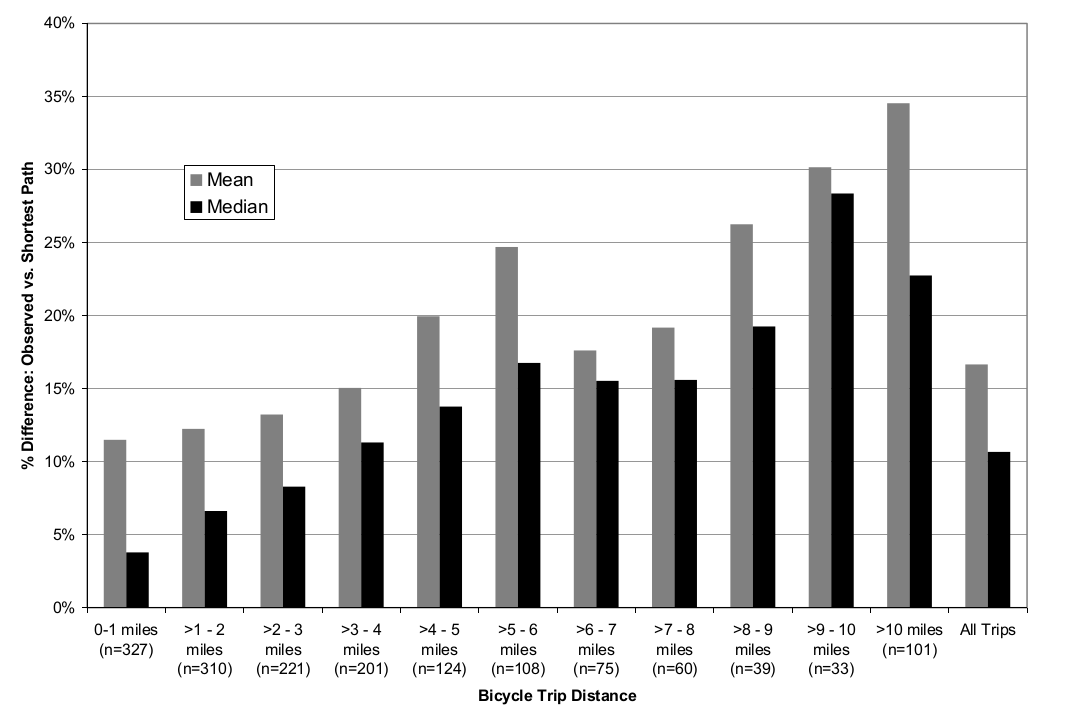
\includegraphics[width=\textwidth]{chapter2/images/deviation_distribution}
\caption{Percent difference between observed and shortest paths by bicycle trip length \citep{dill_understanding_2008}}
\label{fig:dev_dist}
\end{figure}

\begin{figure}
\centering
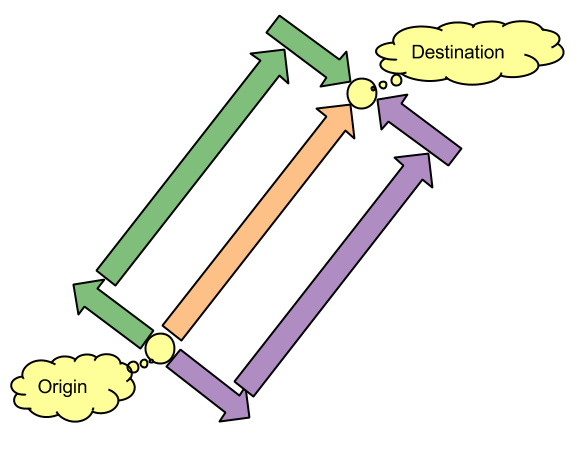
\includegraphics[width=\textwidth]{chapter2/images/zone_of_likely_travel_initiation}
\caption{Initialization of the Zone of Likely Travel}
\label{fig:init_zone}

\centering
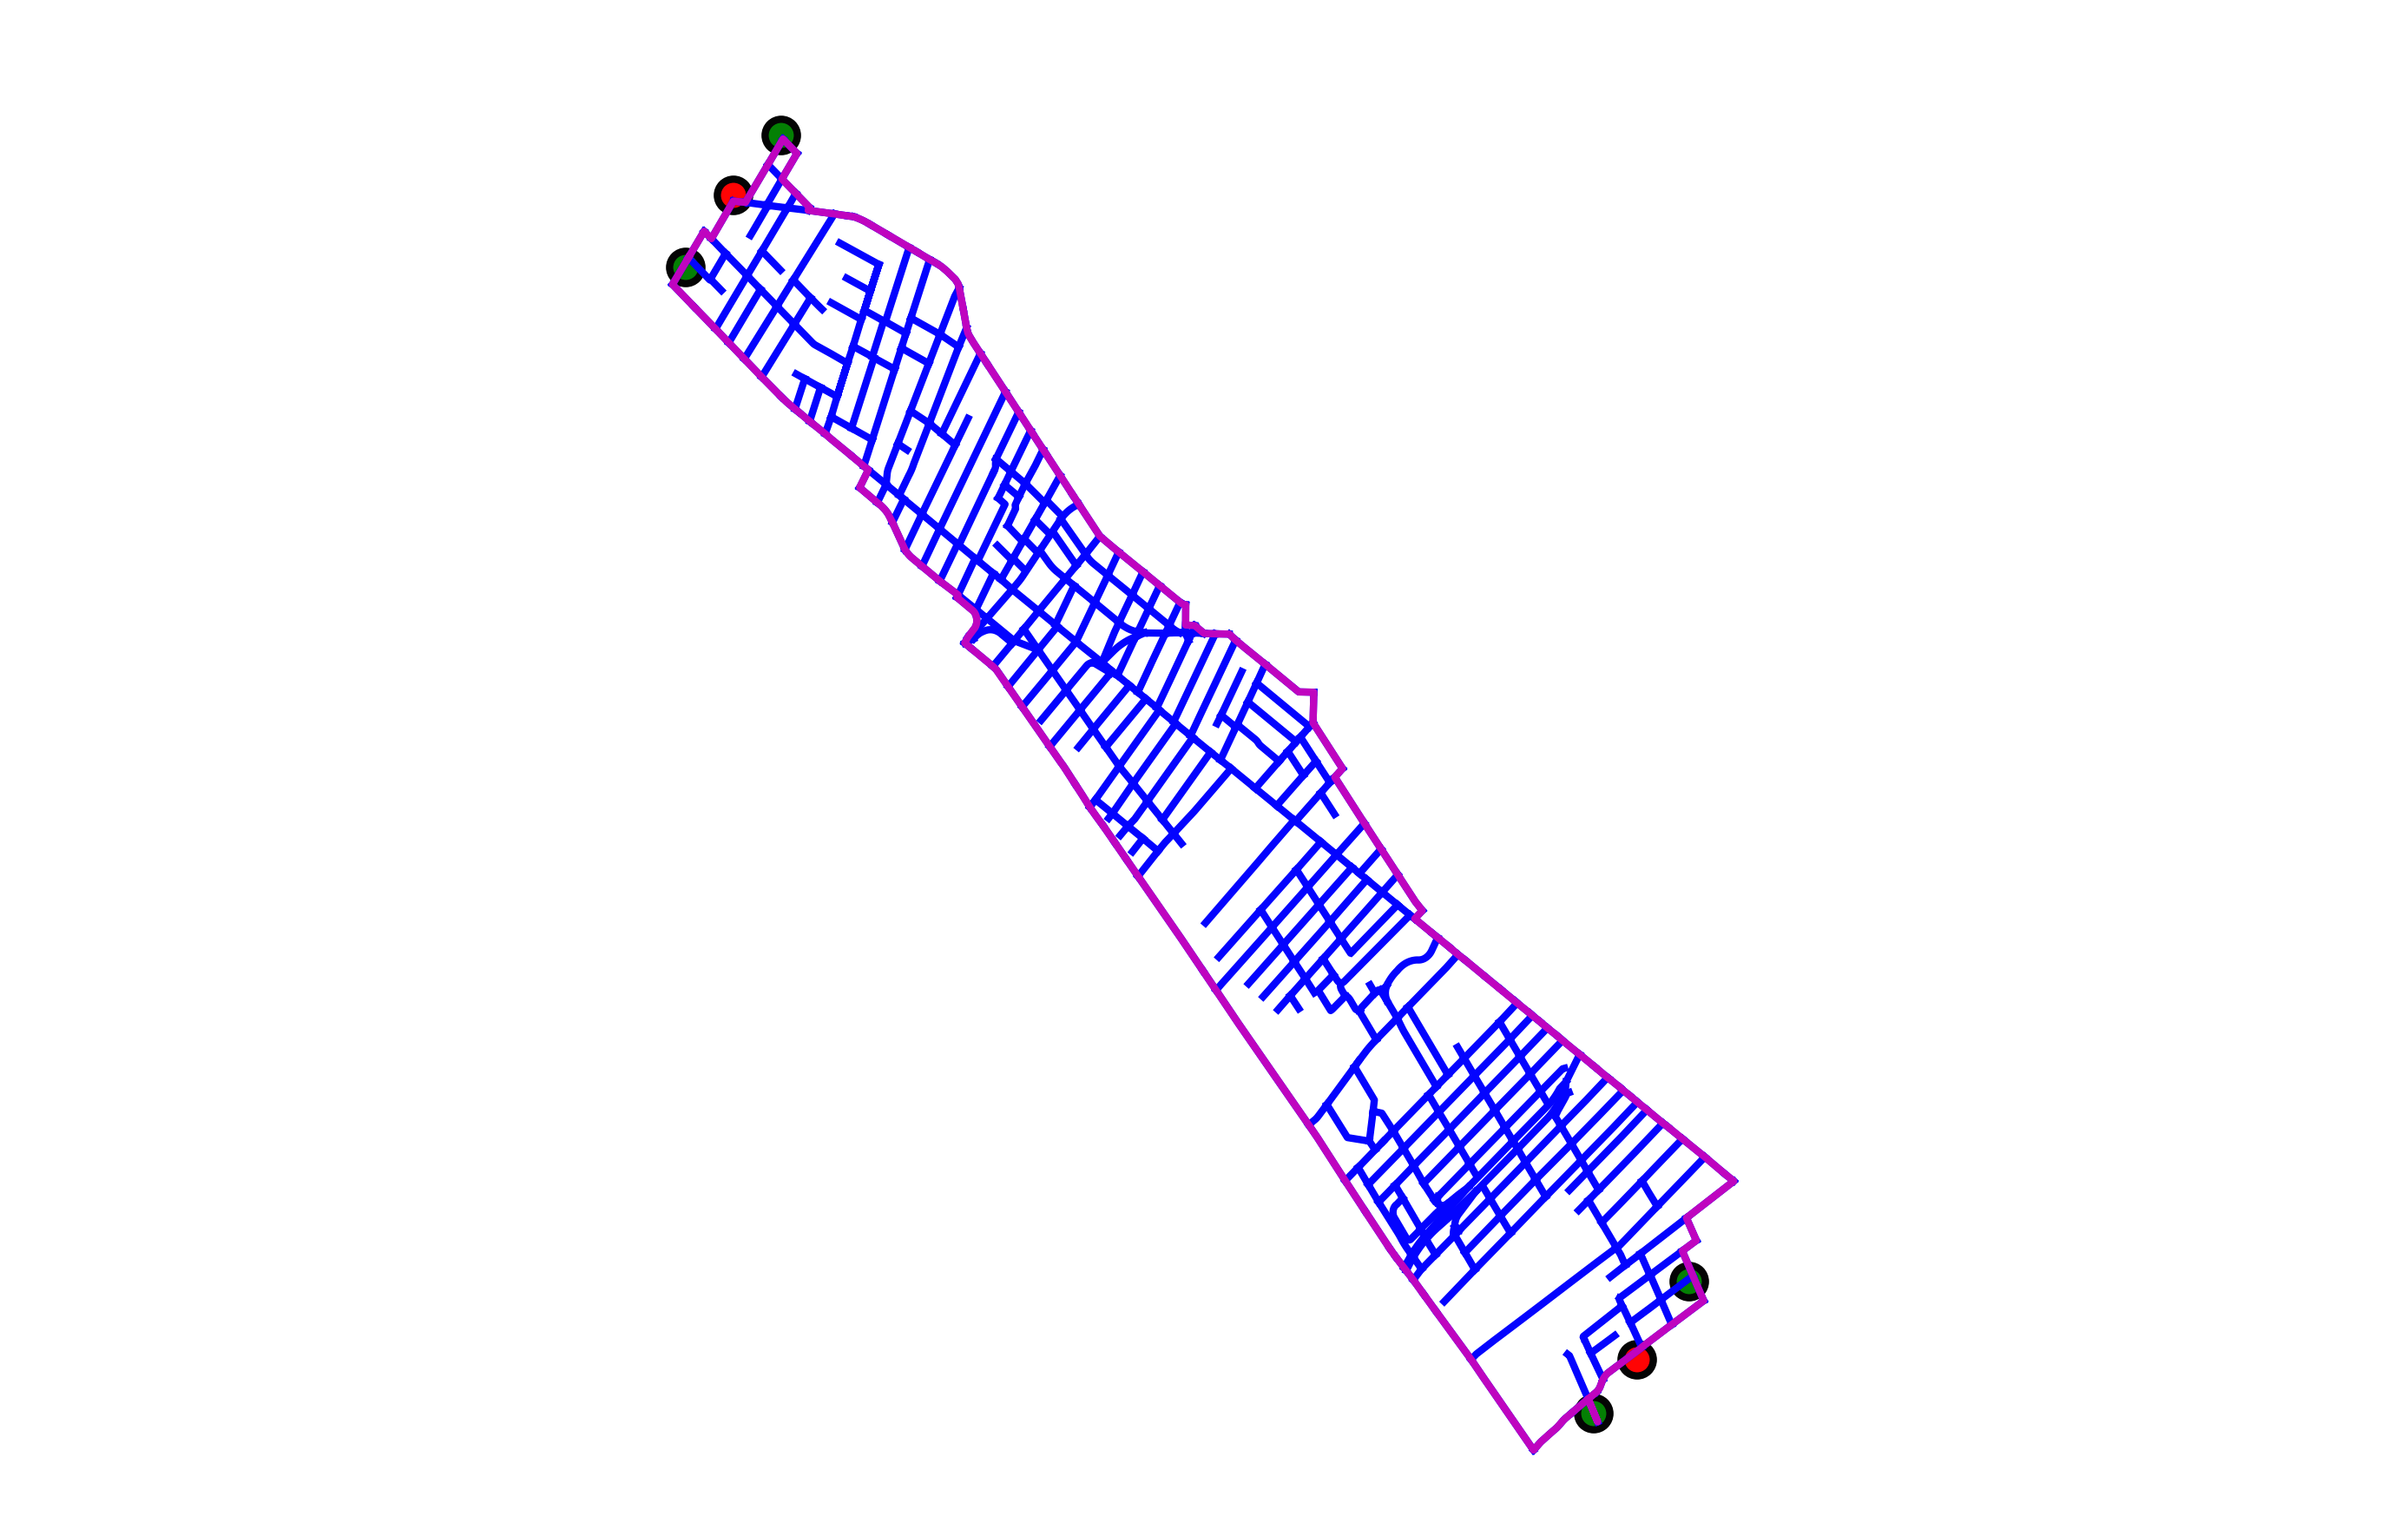
\includegraphics[width=\textwidth]{chapter2/images/zone_example}
\caption{Example of an actual Zone of Likely Travel}
\label{fig:actual_zone}
\end{figure}


\subsection{Decision Trees for Dimensionality Reduction}
\label{sec:trees_for_dimension_reduction}
Given a constructed zone of likely travel, the next step in the methodology is to collect and combine roadway-level variables from the zone in order to describe its bicycling environment. In general, the variables collected from each zone will be determined by the needs, resources, and interest of each researcher. However, the basic idea of this part the methodology is to collect as many variables describing the bicycling environment as one can. 

To determine the variables one collects, one might choose to be creative with one's variable definitions. For instance, one might measure the percentage of miles along the shortest path from one's origin to destination that have speed limits below a certain speed. This would be an indicator of perceived traffic safety along one's most direct travel route. One might also choose to describe the distribution within the zone of each variable of interest as finely as possible. As a concrete example, consider the following. One is often curious about the effects of the following categories of roadway-level variables on the probability that a person chooses to commute by bicycle: types of bicycle lanes, designated bicycle routes, and off-street paths; traffic speeds; traffic volumes; roadway slopes.

The approach that I took in this study was to describe the entire distribution of these variables instead of merely using point  estimates. For example, instead of merely using the mean of all the roadway slopes within the zone, I instead measured the deciles of the empirical distribution of roadway slopes in the zone.

Once one has collected all of the variables that one is interested in, one might have a large corpus of highly correlated variables. For example, I had more than thirty measured variables. As such, directly entering all of these variables into one's mode choice model is not expected to be effective\footnote{Note, this point is corroborated by the results in Table 1 of Chapter 4. There, point estimates of the variables of interest are directly entered into the bicycle utility equation, and still, only the variable for bicycle lanes is statistically significant. Contrast those results to the results shown in Table \ref{table:combined_results} of this chapter where 7 of the 8 dummy variables representing the output nodes of the tree were statistically significant.}. Instead, the variables are combined in a way that reduces the dimensionality of the terms that are added to the mode choice model. Moreover, I wanted the variable combinations to be objective, interpretable, and predictive of whether or not a person choose to commute by bicycle. Because of these requirements, I avoided standard dimensionality reduction techniques such as principle component analysis and factor analysis.These methods have been characterized as difficult to interpret, and the resulting variable combinations are not necessarily predictive of a particular dependent variable. Similarly, I avoided the use of bicycle-environment factors since such factors are constructed subjectively using expert opinions.

The approach I settled on was using a decision tree to perform the variable combination, where the dependent variable was whether or not a person chose to commute by bicycle. Provided that the tree that one constructs is of low depth, the tree and its resultant variable combinations will be easily interpretable. Each output node will be able to read as series of conjunctive statements such as ``this node represents observations whose zones of likely travel meet condition 1 and condition 2 and not condition 3,'' etc. Additionally, because decision trees are constructed with the express purpose of accurately classifying observations, the variable combinations that are created as the decision tree's output nodes will be precisely those that are highly predictive of whether one chooses to commute by bicycle or not. For an in depth discussion of decision trees and strategies for their construction, see Chapter 4.


\subsection{Hybrid Decision Tree-Logit Models}
\label{sec:hybrid_tree_logit_models}
The final step in the methodology is to construct the hybrid decision tree-logit model. As described by \citet{steinberg_hybrid_1998}, this model takes the output nodes of the decision tree and adds them as ``dummy variables'' to the systematic utility of one's discrete choice model. Given that the decision tree is estimated specifically to predict the choice of bicycling or not, I added the dummy variables to the specification of the systematic utility of bicycling as opposed to the utility of any of the other modes.

Now, the main motivation for placing the output nodes of the decision tree into the bicycle utility of one's discrete choice model is to create a link between the effect of the roadway-level variables and the probability that a person bicycles. However, there are other benefits that come from using this technique. First, discrete choice models and decision trees are generally complementary techniques \citep{steinberg_hybrid_1998}. Decision trees work by finding relationships between the dependent variable and local partitions of the space of explanatory variables. In contrast, discrete choice models are typically used to estimate relationships (i.e. the $\beta$'s) that hold globally, for all observations, regardless of one's location in the space of explanatory variables. Given that both techniques have been used to predict discrete outcomes with much success, one may hope to do even better by combining the two techniques. Secondly, the decision tree has (in our case) solely been used to relate the roadway-level variables to the choice of bicycling. Conversely, discrete choice models in transportation usually only account for socio-demographics and level-of-service variables. Combining the two models and re-estimating the coefficients allows us to interpret the effects of roadway-level variable while controlling for socio-demographics and level-of-service and vice versa.

\section{Application}
\label{sec:application}
For an empirical application, I jointly modeled the commute mode choices of individuals in San Francisco, Berkeley, and Oakland. These cities were chosen because I had data on a sample of individual commute mode choices through the 2012-2013 California Household Travel Survey, and because it was feasible for me to acquire, clean, and standardize the needed geospatial data. In the following subsections, I describe the data used in the application, as well as the model specification that is used as my point of comparison. I then present the model results (both the decision tree and hybrid decision-tree logit model), and use the model to forecast the change in the number of bicycle riders that is expected to come from the Telegraph Avenue Complete Streets project in Oakland.

\subsection{Data}
As mentioned above, the primary dataset for this application is the 2012 California Household Travel Survey (CHTS). The CHTS was a one day travel diary taken from a stratified sample of households throughout the state of California and portions of Nevada. It was a stratified sample, one-day travel diary, and it collected detailed information on individual's activities, locations, sociodemographics, household structure, and travel modes. The complete data collection effort is described in \citep{california_department_of_transportation_2010-2012_2013}. From the complete data set, only individuals who both lived and worked or lived and attended school in either Oakland, Berkeley, or San Francisco were extracted and retained for model estimation. 

Beyond filtering based on geography and trip-purpose, I post-processed the raw CHTS data to construct the final dataset used for model estimation. In particular, I combined the data on individual trips into tours, defined a ``chosen travel mode'' for each tour, determined the available travel modes for each tour, and assembled the level-of-service variables for each tour. For this study, I used the level-of-service (travel costs, times, and distance) estimates provided by the San Francisco Metropolitan Transportation Commission (MTC). As a result, the set of possible alternatives in our example was defined to be the same as the categories used by MTC. Specifically, eight travel mode alternatives were specified. There were three driving modes, each differentiated by the number of passengers: drive-alone, shared-ride with two passengers, and shared-ride with three or more passengers. There were also three transit modes, each differentiated by their access and egress modes: walk-transit-walk (where walking is used for access and egress), drive-transit-walk, and walk-transit-drive. Finally, there were two non-motorized modes: walking and bicycling. For each tour, the travel mode that was used for the longest distance was used as the ``chosen travel mode'' for that tour. In total, the final data set included 1,015 tours, 87 of which had bicycling as the primary travel mode used on the tour.

Along with the CHTS data, I drew upon a suite of spatial data from each city and from MTC. Specific data types gathered include street shapefiles, bicycle infrastructure shapefiles, speed limits, topography, traffic analysis zones (TAZs), and city boundaries.

\subsection{Base Model}
The ``basic'' model used for comparison in this chapter is based on MTC's current work-tour mode choice model \citep{san_francisco_metropolitan_transportation_commission_travel_2012}. It is essentially taken ``as-is'' from MTC and is used as a point of comparison for this application. Minor alterations to MTC's model specification were made based on data availability and statistical considerations such as using removing insignificant variables. The largest difference between the MTC model and the model used in this chapter is that I use a multinomial logit model instead of a nested logit model. This decision was made in order to investigate the improvements that are possible in the simplest type of choice model used by MTC. The Maximum Likelihood Estimation (MLE) results of the basic model are presented in Table \ref{table:combined_results}, along wiith the results of the hybrid decision-tree logit model.

\begin{table}
\centering
\begin{tabular}{K{0.5\linewidth} rrrr}
\toprule
{} & \multicolumn{2}{c}{Standard Logit} & \multicolumn{2}{c}{Hybrid Tree-Logit} \\
Variables & \multicolumn{1}{c}{Parameter} & \multicolumn{1}{c}{$t$-Stat} & \multicolumn{1}{c}{Parameter} & \multicolumn{1}{c}{$t$-Stat} \tabularnewline
\midrule

ASC Shared Ride: 2 & -2.737 & -11.833** & -2.717 & -11.715** \\
ASC Shared Ride: 3+ & -2.852 & -12.228** & -2.831 & -12.110** \\
ASC Walk-Transit-Walk & -0.215 & -0.593\hphantom{*}\hphantom{*} & -0.167 & -0.462\hphantom{*}\hphantom{*} \\
ASC Drive-Transit-Walk & -3.414 & -7.332** & -3.370 & -7.237** \\
ASC Walk-Transit-Drive & -3.949 & -8.212** & -3.907 & -8.125** \\
ASC Walk & 1.421 & 5.281** & 1.404 & 5.228** \\
ASC Bike & -0.950 & -3.402** & -3.291 & -5.297** \\
Travel Time, units:min (All Auto Modes) & -0.112 & -7.912** & -0.112 & -7.887** \\
Travel Time, units:min (All Transit Modes) & -0.029 & -6.854** & -0.029 & -6.970** \\
Travel Cost, units:\$ (All Transit Modes) & -0.123 & -1.432\hphantom{*}\hphantom{*} & -0.124 & -1.442\hphantom{*}\hphantom{*}  \\
Travel Distance, units:mi (Walk) & -1.103 & -12.535** & -1.096 & -12.475** \\
Travel Distance, units:mi (Bike) & -0.345 & -7.470** & -0.219 & -4.066** \\
Household Size (Shared Ride 2 \& 3+) & 0.593 & 9.774** & 0.585 & 9.618** \\
Cross-Bay Tour (All Transit Modes) & 1.037 & 2.109*\hphantom{*} & 1.056 & 2.146*\hphantom{*} \\
Node 1 (Bike) & \_ & \_ & 1.402 & 2.816** \\
Node 2 (Bike) & \_ & \_ & 0.926 & 1.066\hphantom{*}\hphantom{*} \\
Node 3 (Bike) & \_ & \_ & 1.928 & 2.369*\hphantom{*}  \\
Node 4 (Bike) & \_ & \_ & 4.238 & 6.338** \\
Node 5 (Bike) & \_ & \_ & 2.370 & 3.798** \\
Node 6 (Bike) & \_ & \_ & 4.583 & 4.931** \\
Node 7 (Bike) & \_ & \_ & 2.612 & 3.585** \\
Node 8 (Bike) & \_ & \_ & 1.483 & 2.145*\hphantom{*}  \\

\multicolumn{5}{c}{}\tabularnewline
Log-likelihood & -1,409.071 & \multicolumn{1}{c}{} & -1,372.327 & \multicolumn{1}{c}{} \tabularnewline

\bottomrule
\multicolumn{5}{l}{Note: * means $\textrm{p-value} < 0.05$ and ** means $\textrm{p-value} < 0.01$.} \\
\multicolumn{5}{l}{\hphantom{Note: }\_ means the corresponding values do not apply to the given model.}\\
\end{tabular}
\caption{Base and Hybrid Decision-Tree Logit Model Results}
\label{table:combined_results}
\end{table}

\subsection{The Hybrid Decision Tree-Logit Model}
As shown by the log-likelihoods in Table \ref{table:combined_results}, the hybrid decision-tree logit model displays a greater in-sample fit to the data as compared to the base model. The greater fit is statistically significant as a log-likelihood ratio test of the hybrid decision-tree logit model versus the restricted base model has a p-value of approximately $1e^{-12}$.

Now, to interpret the results of the hybrid decision tree-logit model, one also needs the estimated decision tree. Figure \ref{fig:tree_results} shows the estimated tree, and Table \ref{table:var_descriptions} describes the names of the variables that appear in the estimated tree.\footnote{Note the variables used to construct the tree include: the percentage of roads having bike lanes on them, the percentage of roads having bike routes or ``share the road'' arrows (i.e. sharrows) on them, the deciles of roadway slopes within a zone, the total elevation change from one's origin to destination, the deciles of roadway speed limits, the length of the shortest path from one's origin to destination, the fraction of one's shortest path that has a speed limit of 20, 30, and 35 miles per hour or higher. Only a subset of these variables appear in the estimated tree shown in Figure \ref{fig:tree_results}.} A few interesting aspects of the hybrid decision tree-logit model are immediately apparent. First, the presence of bicycle lanes only affects those individuals in output nodes 3-5, where the shortest path between the individual's home and work is less than 3.01 miles. This underscores the importance of distance in determining whether an individual chooses to bicycle and whether the individual is strongly impacted by the installation of on-street bike lanes. Secondly, the numerous appearance of the slope variables highlights the importance of having a relatively flat bicycling environment\footnote{Note, basic node splitting procedures for tree construction are biased towards selecting variables (such as the ``slope\_xx'' variables) with many unique values \citep{kim_2001_classification}. However, I was not aware of this fact when conducting the study described in this chapter. Future research should investigate the sensitivity of the decision tree's interpretation to the use of unbiased splitting procedures.}. Finally, it is instructive that the variable at the top of the tree is the fraction of roadways along one's shortest path with roadways of 35 miles per hour or higher. This emphasizes the fact that individuals rarely commute by bicycle in regions where their most direct path is along roads with fast moving (i.e. unsafe) traffic.

\begin{figure}
\centering
    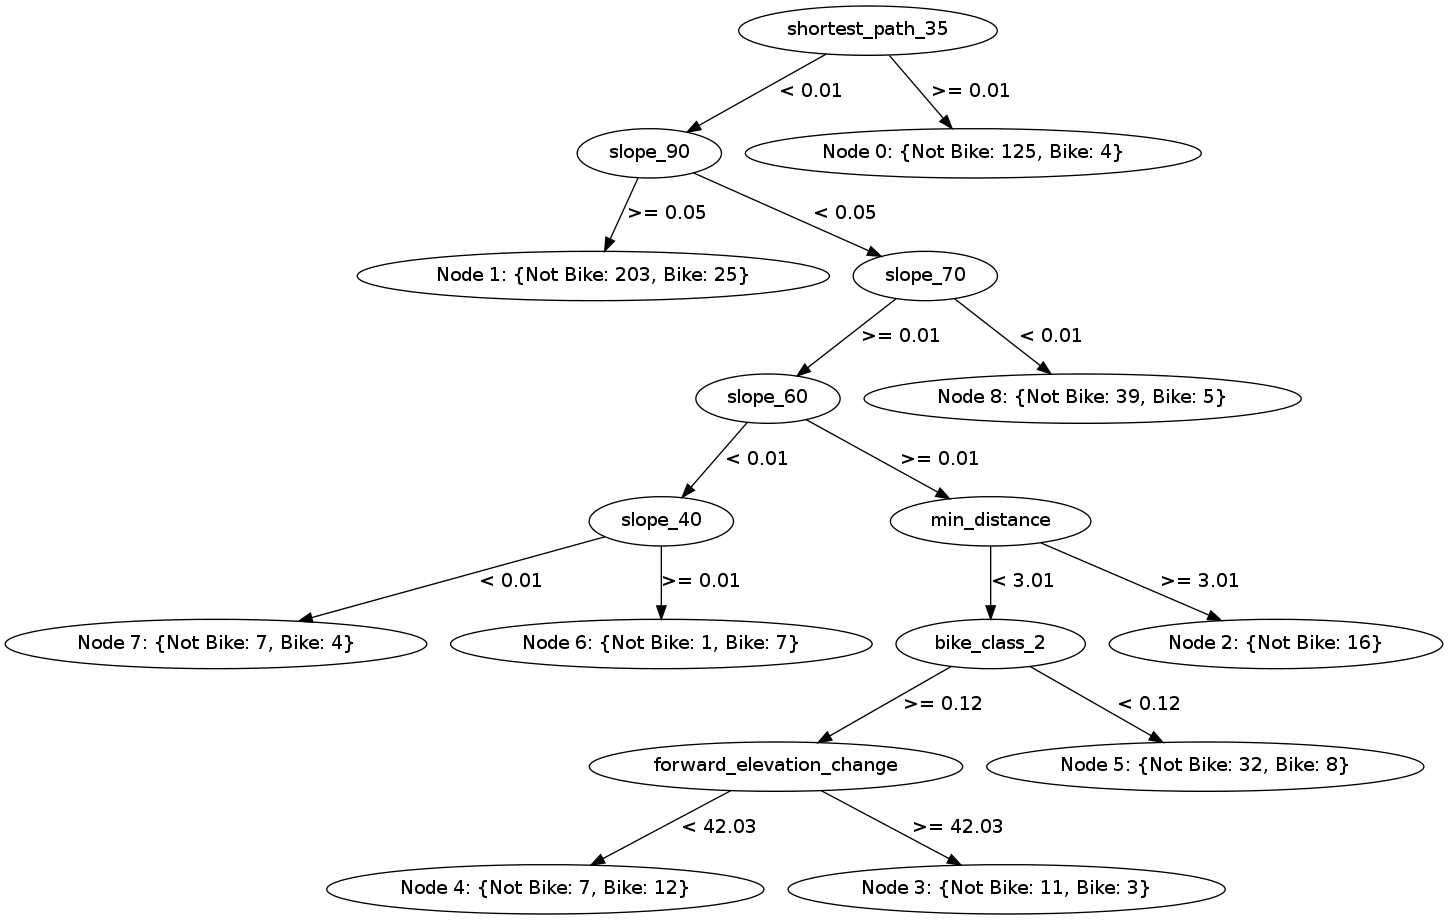
\includegraphics[width=\textwidth]{chapter2/images/test_graph_2}
    \caption{Estimation results for the decision tree}
    \label{fig:tree_results}
\end{figure}

\begin{table}
\begin{tabularx}{\textwidth}{l X}
\toprule
\multicolumn{1}{l}{Variable} & Descriptions \\
\midrule

shortest\_path\_35 & The ratio of miles of 35 mph roadways along the shortest path from one's origin to destination to the total roadway miles along the shortest path. 
 \\[1.2ex]
slope\_xx & The xx-percentile of the slopes in the zone of likely travel between one's origin and destination. 
\\[1.2ex]
min\_distance & The length, in miles, of the shortest path between one's origin and destination. 
 \\[1.2ex]
bike\_class\_2 & The ratio of roadway miles in one's zone of likely travel which have a bike lane on them to the total roadway miles in one's zone. 
\\ [1.2ex]
forward\_elevation\_change  & The absolute value of the change in elevation (in feet) between one's origin and destination. \\ 
\bottomrule

\end{tabularx}

\caption{Variable descriptions for variables in the classification tree}
\label{table:var_descriptions}
\end{table}

While the discussion so far has centered on the in-sample estimation results, I did assess the performance of the proposed methodology using out-of-sample testing. Specifically, I used two complementary metrics to assess the out of sample performance of the proposed method and the traditional logit model without roadway level variables: the out-of-sample log-likelihood and ``sensitivity.'' The log-likelihood measures the overall quality of a model's predicted probabilities. The sensitivity of a model measures the model's discriminative ability---it is the percentage of observations of a given outcome that are correctly classified\footnote{Note, for probabilistic models with multiple outcomes, an observation is classified as having the outcome with the highest predicted probability.} by one's model. Since this study is specifically focused on cycling, the models were judged with respect to their log-likelihoods overall and with respect to their sensitivity towards cycling.

To perform the out-of-sample testing, I used the ``0.632'' bootstrap \citep{efron_1983_estimating, efron_1997_improvements}. A bootstrap approach to out-of-sample testing was used because alternative techniques (e.g. k-fold cross-validation or hold-out sets) were deemed less appropriate. My intuitions behind the choice of testing procedure were based on the arguments made in \citeauthor{efron_1997_improvements}'s ``Improvements on cross-validation: The .632+ boot-strap methods'' and \citeauthor{japkowicz_evaluating_2011}'s ``Evaluating Learning Algorithms: A Classification Perspective'' (\citeyear[Ch. 5]{japkowicz_evaluating_2011}). These two sources suggested that my dataset's relatively small size (1,015 observations), its highly imbalanced nature (e.g. there were only 87 cyclists), and the expectation of multiple cycling sub-populations or ``small disjuncts'' (e.g. see the popular construct of ``Four Types of Cyclists'' \citep{geller_four_2006}) would lead to high variance in the error-estimates produced by cross-validation and high-bias in the error-estimates produced by a holdout set.

Bootstrapping seemed to strike a useful balance between these bias/variance concerns. For instance, a hold-out set would have resulted in either few cyclists in the held-out group or too few observations overall in the training set. Similarly, the small number of cyclists in each fold of cross-validation would have been expected to increase the variance of all the out-of-sample estimates. Compared to a hold-out set, bootstrapping would maintain the number (though not the information content) of cyclists in the training data. Compared to cross-validation, bootstrapping would generally lead to a higher number of cyclists in the out-of-sample tests and lower variance in the error estimates due to averaging over more error estimates.

Amongst the possible bootstrap methods, I selected the 0.632 bootstrap to perform the out-of-sample testing. This method takes a weighted average between the out-of-sample metrics computed on the bootstrap samples and the in-sample metrics computed on the same training data that one's model was estimated with. The weights are 0.632 for the out-of-sample metrics and 0.328 for the in-sample metrics, and they are derived from the expected percentage of data points that are present in each bootstrap sample. The weights balance the pessimism of the bootstrapped error estimates that are based on less information than one's final model and the optimism of the in-sample metrics that use the same data for estimation and testing. This method was chosen over methods such as the ordinary bootstrap because the 0.632 bootstrap has empirically been shown to accurately estimate prediction error rates in small-samples \citep{efron_1983_estimating, efron_1997_improvements, japkowicz_evaluating_2011}. However, I do note that ``[...] the relative appropriateness of one sampling scheme [e.g. cross-validation, bootstrap resampling, etc.] over the other is classifier dependent'' \citep[p. 183]{japkowicz_evaluating_2011}. Because of this, future research should perform real and simulated studies to investigate what the best type of out-of-sample error estimation technique is for hybrid decision tree-logit models.

Justifications aside, the out-of-sample testing procedure was as follows. I used 2,000 stratified bootstrap samples of the data to re-estimate the models based on this chapter's proposed methodology and the traditional logit model. Each time, the log-likelihood and sensitivity were calculated for the observations that were not part of the bootstrap sample. The out-of-sample log-likelihood and sensitivity metrics were then averaged across the 2,000 bootstrap samples. Finally, a weighted average was taken between the in-sample metrics and the the average metrics for the bootstrap samples. Following the 0.632 bootstrap procedure \citep[pp. 181-182]{japkowicz_evaluating_2011}, the weights were 0.368 and 0.632 for the in-sample and out-of-sample metrics, respectively.

\begin{table}
\centering
\begin{tabular}{K{0.5\linewidth} rr}
\toprule
Metrics & Standard Logit & Hybrid Tree-Logit \tabularnewline
\midrule

Log-Likelihood & -1,421.0 & -1,392.6\\
Sensitivity (Cyclists) & 3.5 & 33.7\\

\bottomrule
\end{tabular}

\caption{Out-of-Sample Results for the Base and Hybrid Decision-Tree Logit Models}
\label{table:oos_results}
\end{table}

Table \ref{table:oos_results} shows the results of these procedures. Consistent with the in-sample results, this chapter's proposed methodology leads to better probabilistic predictions and greater discriminatory power, even out-of-sample\footnote{Note, the out-of-sample results suggest, rather than prove, that the hybrid decision tree-logit generalizes better than the standard MNL model. In particular, the logit coefficients were re-estimated during the bootstrapping procedure. However, the decision tree itself remained constant, thus providing an avenue for potential over-fitting. That said, two features of the tree estimation procedure reduce the likelihood of over-fitting. First, a minimum number of 5 observations had to be contained in a given output node in order for the node to be created. This should play a small role in reducing the chance that the decision tree was overly affected by noise in the data that does not generalize to unseen observations. The second, and more substantial, feature is that ``reduced error pruning'' \citep{rokach_decision_2005} was used to arrive at the tree shown in Figure \ref{fig:tree_results}. This procedure removes output nodes that lead to increased error on a set of held-out data (i.e. a 20\% stratified sample of the original dataset) that was not used to estimate the initial tree. In this sense, even though the tree shown in Figure \ref{fig:tree_results} was not re-estimated during the bootstrapping procedure, this tree should already be somewhat inoculated against over-fitting to the estimation data.}. The improvements in sensitivity are especially encouraging. For bicycle planning, infrastructure installation decisions must specify where in space that infrastructure will be installed. To make such siting decisions optimally, it is important that one's model be accurate at an individual level. One characteristic of a model that is accurate at the individual level is that the model will be able to accurately identify the alternative with the highest probability for each person. Thus, the model's sensitivity should be high. Given that the hybrid decision tree-logit model has a much higher out-of-sample sensitivity than the traditional logit model, I believe the proposed model should also be much more useful for planning purposes.

\subsection{Policy Forecast}
Finally, to demonstrate the responsiveness of the hybrid decision tree-logit model to policy-relevant decisions, I used the Telegraph Avenue Complete Streets Plan as a case study. The context for this case study is that, in 2014\footnote{Note, the work described in this chapter was performed in 2014, before design and construction decisions for the Telegraph Avenue project were finalized.}, the City of Oakland, California was planning to redesign Telegraph Avenue between 20th Street and 57th Street. The Complete Streets Plan had two design options. Option one was to install bicycle lanes between 20th Street and 46th Street, sharrows between 46th Street and 52nd Street, and bicycle lanes between 52nd Street and 57th Street. Option two proposed a protected cycle track from 20th Street to 46th Street, bicycle lanes between 46th Street and 52nd Street, and protected cycle tracks from 52nd Street to 57th Street.

At the time the 2013 CHTS data was collected, the one protected bicycle lane in San Francisco was outside of the zone of likely travel for any of the observations in my dataset, and there were no protected bicycle lanes in Oakland or Berkeley. As a result, it was not feasible to analyze or forecast the effect of installing protected bicycle lanes as opposed to traditional bicycle lanes. Such an analysis would involve extrapolation beyond the range of the observed data, and this analysis would likely lack credibility. Instead, I chose to test design option one as it was described and to test a worst case scenario for design option two. The worst case scenario for design option two would be that the protected bicycle lanes only conferred as much of a benefit as installing a regular bicycle lane.

Given the aforementioned policy scenarios and the sample weights provided by the CHTS, I used sample enumeration to forecast the change in bicycle demand that would occur among people who live in Oakland and work in Oakland, Berkeley, or San Francisco if design option one or two was selected. Note, my worst-case scenario simply takes option two from the Complete Streets plan and replaces the protected cycle tracks with bicycle lanes. This implements the worst-case assumption that the effect of cycle tracks on bicycle demand is the same as a bicycle lane. To summarize, the two scenarios that were forecasted were: (i) installing bicycle lanes on Telegraph Avenue between 20th Street and 46th Street, sharrows between 46th Street and 52nd Street, and bicycle lanes between 52nd Street and 57th Street, and (ii) installing bicycle lanes on Telegraph Avenue between 20th Street and 57th Street with no interruption.

The forecast results are shown in Figures \ref{fig:forecast_results}. Of the individuals who live in Oakland and work in Oakland, Berkeley, or San Francisco, 153 individuals and 469 individuals, respectively, were forecast to begin bicycle commuting as a result of design option 1 and the worst-case scenario described above for option two. In terms of the effects on Oakland's bicycle mode shares, the 2014 mode shares were expected to change from 6.42\% to 6.64\% under design option one and from 6.42\% to 7.10\% under the worst-case scenario for design option two.

\begin{figure}
\centering
    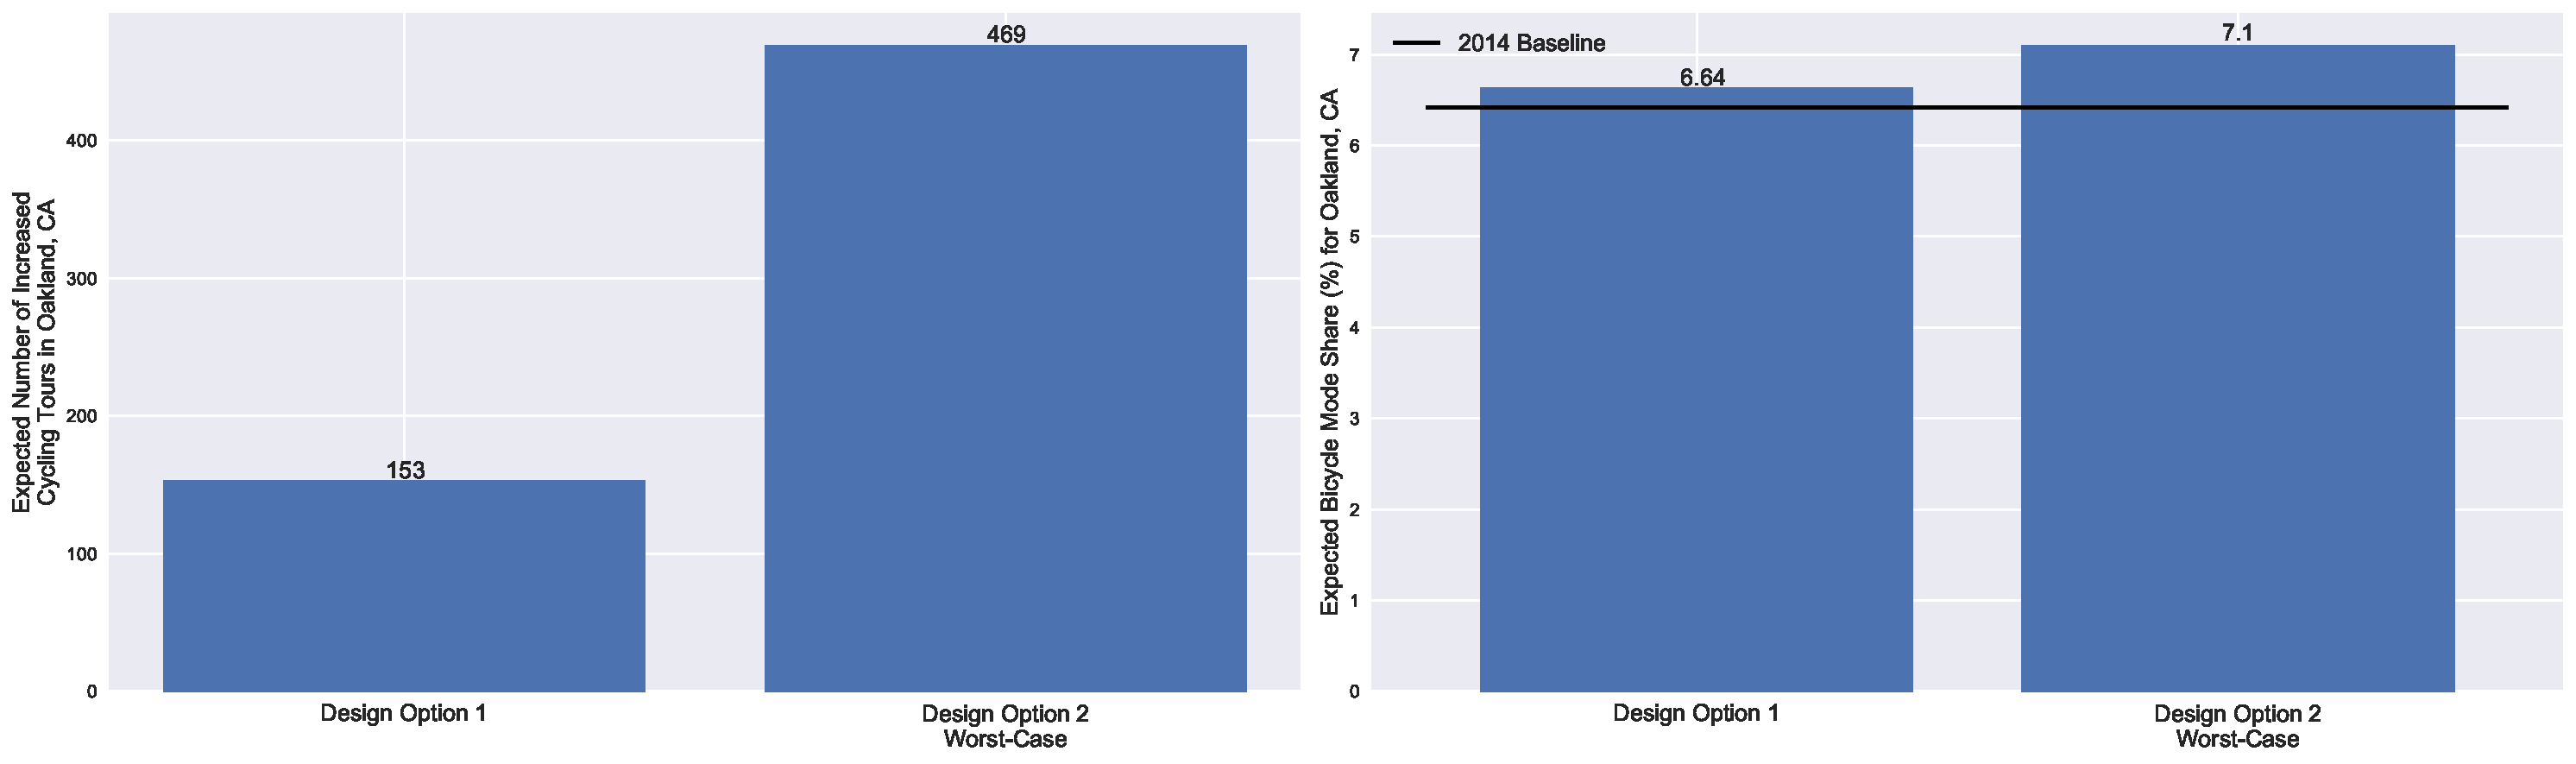
\includegraphics[width=\textwidth]{chapter2/images/forecast_results}
    \caption{Forecast results for the hybrid decision tree-logit model}
    \label{fig:forecast_results}
\end{figure}

There are two main findings from this exercise. First, the substantive finding is that keeping the bike lanes on Telegraph Avenue from 46th to 52nd Streets makes a large difference in terms of bicycle demand because that roadway segment is likely to be traversed by many potential cyclists and because sharrows were not associated with a high levels of bicycle usage. Secondly, the methodological finding of this case study is that the combined zone of likely travel and hybrid tree-logit model is sensitive to roadway level variables, as expected. As shown by this case study, the proposed methodology is responsive to changes as small as replacing 6 blocks worth of sharrows with bicycle lanes.

\section{Conclusion}
\label{sec:conclusion}
In this chapter, I introduced a method for incorporating roadway-level variables into discrete choice models. Intuitively, the proposed methodology works as follows. First, for each individual, a geographic buffer is drawn around the shortest path between the individual's origin and destination. The buffer size is chosen so that the buffer contains the roadways that an individual is likely to traverse if the individual were to bicycle. The region denoted by this buffer is referred to as the ``zone of likely travel.'' Next, for all roadways in the zone, the variables of interest are calculated (e.g. does tthis roadway have a bicycle lane, what is the speed limit on this roadway, etc.). These variables are then aggregated to the level of the zone. In this chapter, such aggregation was done by computing deciles of continuous variables and means of continuous and discrete variables. After variable aggregation, each zone of likely travel was ``scored'' by a decision tree. The decision tree was constructed by using whether each individual bicycled as the dependent variable and using the aggregated variables for each zone as explanatory variables. Since each ``score'' is a mapping from a particular output node of the decision tree, membership in each output node was added to the bicycle utility function of a traditional discrete choice model using dummy variables.

Section \ref{sec:zone_of_likely_travel} highlighted the ways that the proposed methodology addresses theoretical shortcomings of previous methods. Empirically, Section \ref{sec:application} showed that the new procedure out-performed traditional discrete choice models that failed to incorporate roadway-level variables and that these performance improvements held both in-sample and out-of-sample and with multiple metrics. Finally, the case study showed that the proposed technique is sensitive to the roadway-level variables and their spatial configuration---sensitive enough to show real differences between two proposed bicycle infrastructure investments in Oakland, California.

All together, this chapter presents a new method for incorporating roadway level variables into discrete choice models. The proposed methodology has expected theoretical benefits over other methods for incorporating roadway-level variables into discrete choice models, and there are empirical benefits to be gained over not incorporating such roadway-level variables. Hopefully, future work will lead to more case studies of the proposed methodology and also to quantitative comparisons with methods based on geographic buffers around points, bicycle-environment factors, and combined route and mode choice models. From a methodological standpoint, it would also be interesting to investigate the extent to which this chapter's proposed methods is able to reduce the spatial dependence of the residuals from one's choice models.

\newpage
\renewcommand\bibname{{References}} %  will print ''References'' instead of ''BIBLIOGRAPHY''
\bibliographystyle{plainnat}
\bibliography{chapter2/current/ch2}

%\clearpage
%!TEX root = ../../../dissertation.tex

\chapter{Asymmetric, Closed-Form, Finite-Parameter Models of Multinomial Choice}
\label{ch:3}

\begin{chapterabstract}
Class imbalance, where there are great differences between the number of observations associated with particular discrete outcomes, is common within transportation and other fields. In the statistics literature, one explanation for class imbalance that has been hypothesized is an asymmetric (rather than the typically symmetric) choice probability function. Unfortunately, few relatively simple models exist for testing this hypothesis in transportation settings---settings that are inherently multinomial. This chapter fills this gap.

In particular, we address the following questions: ``how can one construct asymmetric, closed-form, finite-parameter models of multinomial choice'' and ``how do such models compare against commonly used symmetric models?'' Methodologically, we introduce (1) a new class of closed-form, finite-parameter, multinomial choice models, (2) a procedure for using these models to extend existing binary choice models to the multinomial setting, and (3) a procedure for creating new binary choice models (both symmetric and asymmetric). Together, our contributions allow us to create new asymmetric, closed-form, finite-parameter multinomial choice models. We demonstrate our methods by developing four new asymmetric, multinomial choice models. Empirically, most of our models strongly dominate the multinomial logit (MNL) model in terms of in-sample and out-of-sample log-likelihoods. Moreover, analyzing two policy applications, we find practical differences between the MNL and our new asymmetric models. Our results suggest that while asymmetric models may not always outperform symmetric ones, asymmetric choice models are worth testing because they might have better statistical performance and entail substantively different policy and financial implications when compared with traditional symmetric models, such as the MNL.
\end{chapterabstract}

\section{Introduction}
\label{sec:intro}
Discrete choice modeling is widely used in transportation. It is used in every area of travel demand analysis, such as residential choice, work location choice, destination choice, time-of-travel choice, mode choice, and route choice. Moreover, discrete choice modeling is also used outside of transportation in  fields such as marketing, economics, finance, operations research, statistics, and medicine. Across these many disciplines, the most commonly used models have fairly simple functional forms, such as the multinomial logit (MNL) and binary logit models. The use of simple models is, in part, due to the greater computational burdens required to estimate and forecast with very general discrete choice models. Clearly then, it is important to create simple models that are nonetheless able to avoid unwanted properties of classic models such as the MNL model. In this chapter, we introduce models that have the same basic form as the MNL model but, for the price of a finite number of new parameters that are to be estimated from the data, provide potentially much better fits to one's data and avoid a ``symmetry property'' that we argue is often undesirable. The next paragraph will review the MNL model because it is the starting point for the class of models that we introduce. Then, we will describe the symmetry property, show it is present in common discrete choice models, and make the case that such a property is not always desirable.

While the MNL and binary logit models are often used because of their ease of estimation, their closed-form probability equations (shown in Equation \ref{eq:mnl_formula})\footnote{Note that the variables are fully listed in order to make clear the notation used in the chapter.}, and their ease of interpretation, their use requires analysts to accept a set of properties that may be overly restrictive or inaccurate in the specific contexts being modeled. Specifically, one well known property is known as Independence from Irrelevant Alternatives (I.I.A.). The I.I.A. property is seen as problematic when one considers substitution patterns between alternatives that are closely related, and there have been numerous models that aim to avoid I.I.A. (e.g. nested logit, cross-nested logit, etc.).

\begin{equation}
\label{eq:mnl_formula}
\begin{aligned}
P \left( y_{ij} = 1 | V_{i1}, V_{i2}, ..., V_{ik} \ \forall \left\lbrace j, k \right\rbrace \in C_i \right) &= \frac{\exp \left( V_{ij} \right)}{\sum _{\ell \in C_i} \exp \left( V_{i \ell} \right)} \\
\textrm{where } y_{ij} &= \textrm{a binary (0 or 1) indicator of whether individual $i$} \\
&\quad \  \textrm{is associated with outcome $j$.} \\
C_i &= \textrm{the choice set for individual $i$} \\
V_{ij} &= x_{ij} \beta = \textrm{the index for alternative $j$ for individual $i$} \\
\beta &= \textrm{a column vector of unknown population parameters} \\
x_{ij} &= h \left( z_j, \zeta _i \right) \textrm{, a row vector.} \\
h \left(  \right) &= \textrm{a function that returns a row vector} \\
z _j &= \textrm{attributes of alternative $j$ for individual $i$} \\
\zeta _i &= \textrm{characteristics of individual $i$}
\end{aligned}
\end{equation}

In addition to the I.I.A. property, the MNL model's probability function also implies a ``symmetry property.'' Specifically, from a point where an individual has a 50\% probability of choosing an alternative $j$, this probability will increase and decrease at equal rates with respect to equal-magnitude increases and decreases in alternative $j$'s index, $V_{ij}$. Probability functions with this quality are henceforth referred to as symmetric, and probability functions without this property are henceforth referred to as asymmetric. See Figure \ref{fig:symm_logit_probit} for a visual depiction of symmetric and asymmetric probability functions. The binary, complementary log-log model (henceforth clog-log model) is described in Section \ref{sec:deriving_multinomial_cloglog} and used in Figure \ref{fig:symm_logit_probit} as an example of an asymmetric probability function. In contrast, the binary logit and binary probit models are used as examples of symmetric probability functions. Note that the logit model is not the only model with the symmetry property. The other commonly used discrete choice model, the simple probit model\footnote{The `simple' probit model assumes that the error terms of the utility of each alternative are independent and identically distributed.}, is also symmetric. The point being made here is that while it is seldom spoken of, a basic property of standard discrete choice models is that one's probability of choosing a given alternative is symmetric about 50\%, with respect to the index, $V_{ij}$, of that alternative.

\begin{figure}
\centering
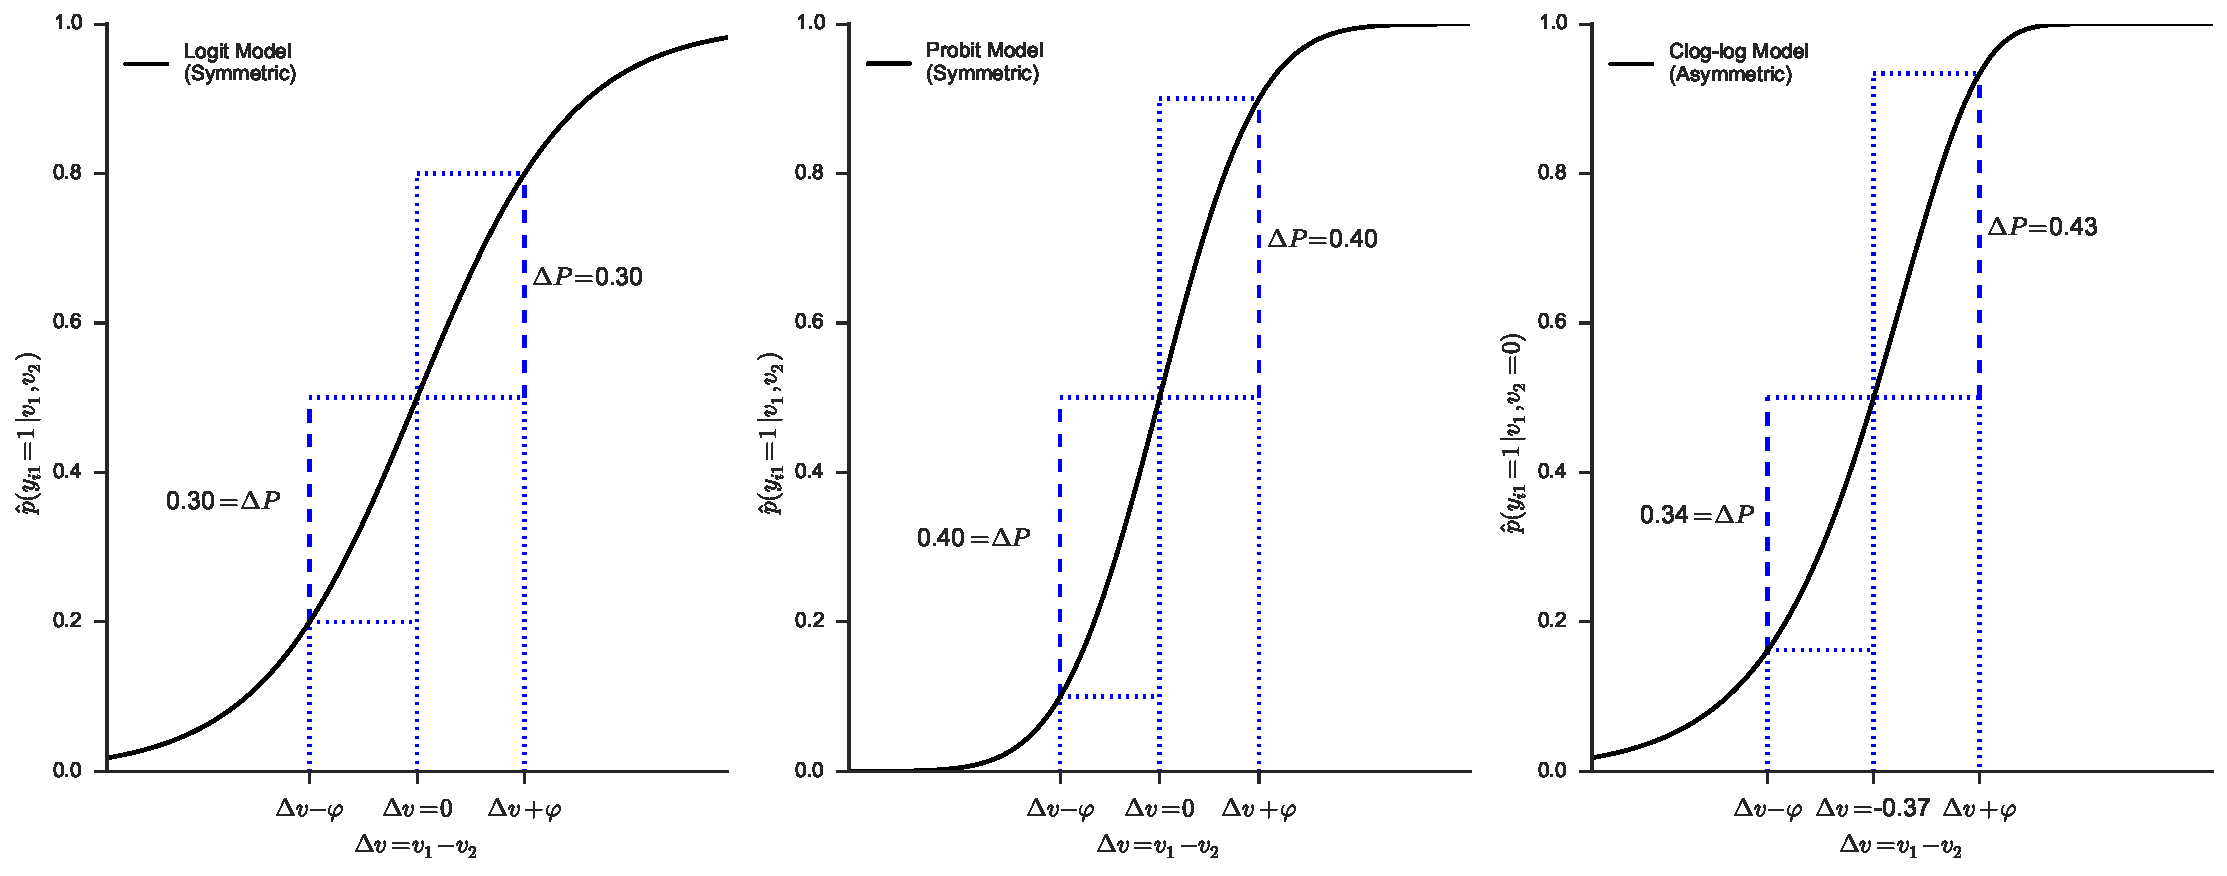
\includegraphics[width=\textwidth]{chapter3/images/Fig1_600dpi}
\caption{Symmetric and Asymmetric Binary Choice Probability Functions}
\label{fig:symm_logit_probit}
\end{figure}

Although models exhibiting the symmetry property are pervasive in discrete choice modeling, there are situations where such a property may seem overly restrictive. Class-imbalanced choice contexts, where the numbers of observations choosing each alternative are unequal, are one such set of situations. Note that in transportation, class-imbalanced choice contexts are ubiquitous. For example, in the United States (US), there are almost always many more automobile drivers than bicyclists when modeling commute mode choices. Furthermore, while the initial motivation and focus of our empirical applications is on travel mode choice, we emphasize that class imbalance is prevalent in many settings where discrete choice models are employed. For instance, class imbalance is observed in: biomedical studies of the dose-response effects of drugs \citep{pregibon_goodness_1980}; destination choice studies in the form of 'superstar' destinations \citep{chorus_paving_2016}; loan default studies \citep{calabrese_modelling_2013}; and studies of shoppers' brand choice \citep{briesch_semiparametric_2002}.

In class-imbalanced situations, it might be natural to hypothesize that the probability of choosing the under-represented alternative decreases more rapidly from 50\% than it increases, even for equal-magnitude decreases and increases in the alternative's index, $V_{ij}$. In other words, it might be natural to think that different alternatives have differing rates of adoption and abandonment. Of course, this hypothesis is not the only plausible explanation for the observed class imbalance\footnote{As noted by one referee, there are numerous methods in use in statistics and machine learning for ameliorating the effects of class imbalance on one's chosen performance metric. For example, there exist many types of over- and under-sampling techniques. These techniques deal with the effect of class imbalance on \textit{prediction}. The focus of this chapter is different. We use asymmetric probability models to accommodate alternative \textit{explanations} of why class imbalance is observed.}. The point, however, is that symmetric probability models prohibit one from investigating hypotheses about the magnitude of changes in the probability of choosing an alternative, from a probability of 50\%, with respect to equal-magnitude increases and decreases in that alternative's index. This is because symmetric probability models assume \textit{a-priori} that the changes in probability are equal. 

In light of this undesired symmetry property of common discrete choice models such as the standard MNL and simple probit model, this chapter's contributions to the transportation and discrete choice literature are that it:
\begin{enumerate}
\item introduces a general class of closed-form, finite-parameter models for multinomial choice situations that do not necessarily imply symmetric choice probability functions (as well as four new models within that class),

\item introduces and demonstrates a methodology for
    \begin{enumerate}
        \item extending existing, binary choice models to the multinomial setting and
        \item creating new binary choice models (both asymmetric and symmetric),
	\end{enumerate}

\item demonstrates that asymmetric probability models can substantially improve upon the fit of standard discrete choice models such as the MNL model, and
 
\item shows that, compared to symmetric models such as the MNL model, asymmetric choice probability functions can lead to substantive differences (both quantitatively and qualitatively) in one's resulting statistical inference and policy-analyses.
\end{enumerate}

For clarity, we reiterate the main purpose of this chapter. First, we note that class imbalance is a common occurrence in discrete choice analyses. Secondly, through extensive reference to the existing statistical literature, we highlight the fact that asymmetric probability functions have been given as \textit{\textbf{one possible}} explanation for why there might be low relative numbers of individuals choosing a particular alternative \citep[p. 1172]{chen_new_1999}. Another possible explanation is a data-generating process with a symmetric probability function and low, average systematic utilities in one's population for the under-represented alternatives, relative to the over-represented alternatives. In general, we do not think that class imbalance \textit{\textbf{necessarily}} implies an asymmetric probability function\footnote{Additionally, this paragraph does not imply that $P \left( \textrm{asymmetry} \mid \textrm{class imbalance} \right)$ $> P \left( \textrm{symmetry} \mid \textrm{class imbalance} \right)$ or that $P \left( \textrm{asymmetry} \mid \textrm{class imbalance} \right)$ $> P \left( \textrm{asymmetry} \mid \textrm{balanced classes} \right)$. Indeed, it is possible that asymmetric choice models may be of use in scenarios where one's classes are balanced. Instead, this paragraph's sole purpose is to describe the reasoning that motivated this paper, even if such reasoning may be incomplete or otherwise flawed. Future research should formally investigate the conditions under which asymmetric choice models are to be preferred to symmetric choice models. It may turn out that such conditions have nothing to do with class imbalance. Either way, the research question of when asymmetric choice models are most useful is not studied in this paper.}. Moreover, we do not think that asymmetric probability functions will \textit{\textbf{necessarily}} perform better than symmetric ones when modeling class imbalanced data. Investigation of such claims are beyond the scope of this chapter. Through reference to the existing statistical literature, and through our empirical applications, we instead demonstrate that asymmetric probability functions \textit{\textbf{can possibly}} provide better explanations of the observed choices in one's class imbalanced dataset, and that due to this possibility, one should investigate the use of asymmetric probability functions in one's analyses. To facilitate the use of asymmetric probability functions in discrete choice analyses, we create methods to construct new, binary probability functions (both symmetric and asymmetric), and we create methods to extend binary probability functions to the multinomial settings that are common in many fields that use discrete choice models.

The rest of the chapter is organized as follows. Section \ref{sec:lit_review} will review related literature and current approaches to producing discrete choice models that are not necessarily symmetric. Section \ref{sec:logit_type_models} will detail our proposed class of choice models, relate it to the existing literature, and show how one might create such models. Section \ref{sec:model_estimation} will describe the estimation procedures for our proposed models, and Section \ref{sec:empirical_applications} will detail our empirical examples and case studies, comparing our proposed models to existing ones such as the MNL model. Section \ref{sec:extensions} will discuss extensions of our work and Section \ref{sec:conclusion} will conclude.

\section{Literature Review}
\label{sec:lit_review}
One can partition the asymmetric discrete choice models that have been proposed in the literature based on whether they:
\begin{itemize}
\item are binary or multinomial choice models,
\item are closed- or open-form\footnote{The probability equation of open-form models contain analytically intractable integrals or infinite sums.} models,
\item have a null, finite, or infinite\footnote{Models with an infinite number of parameters are known as non-parametric or semi-parametric models.} set of shape parameters---i.e. parameters that control the shape of the resulting choice probability function.
\end{itemize}
To review the literature that this chapter builds upon, we will iterate through each of these descriptors in the coming paragraphs---describing the work that has been done so far, how that work relates to or has been used in transportation, and issues with the existing literature that our chapter addresses.

First, virtually all research that explicitly focuses on the development of asymmetric choice models has been carried out in the binary setting. Since at least 1976, statisticians and computer scientists have been introducing closed-form, asymmetric generalizations of the standard binary logit model through the use of one or two shape parameters \citep{prentice_generalization_1976, pregibon_goodness_1980, aranda-ordaz_two_1981, guerrero_use_1982, stukel_generalized_1988, morgan_extended_1988, czado_link_1992, czado_parametric_1994, nagler_scobit:_1994, chen_new_1999, vijverberg_betit:_2000, masnadi-shirazi_variable_2010, vijverberg_pregibit:_2012, nakayama_unified_2015, komori_asymmetric_2015}. These shape parameters allow one to adapt the shape of the resulting choice probability function to fit the data at hand. Beyond generalizations of the logit model, a number of binary, asymmetric models that do not nest the logit model have also been proposed in the statistics literature. For example, the clog-log model has been around since at least the 1920s \citep{fisher_mathematical_1922, yates_use_1955, mccullagh_generalized_1989}, and the GEV regression model (not to be confused with McFadden's GEV distribution) is a generalization of the clog-log model with one shape-parameter \citep{wang_generalized_2010, calabrese_modelling_2013}. Still other asymmetric models of binary choice have been introduced based on skewed normal distributions \citep{bazan_framework_2010}, skewed student's t-distributions \citep{kim_binary_2002, kim_flexible_2008}, and symmetric power distributions \citep{jiang_new_2013}. Broadly, the binary choice models with one or more shape parameters have been referred to as ``parametric link functions'' in the statistics literature \citep{mccullagh_generalized_1989}, and many examples of asymmetric choice models can be found by searching for scholarly articles that use such phrases.

Two problems exist with the asymmetric choice models just discussed. First, while the litany of binary, asymmetric choice models that has been developed may be quite useful, they must be extended to the multinomial setting for use in transportation contexts---contexts where the choice situations are often inherently multinomial. Secondly, the proliferation of binary, asymmetric choice models suggests that no single asymmetric model fits the needs of all researchers. However, no guidance on how to create such asymmetric models has been offered in the literature. The various models cited in the last paragraph were almost all introduced without any explanation of where the functional form for the model came from. Sections \ref{sec:logit_type_models} resolves these issues by detailing a method for extending binary, asymmetric models to the multinomial setting and by introducing a methodology for creating binary, asymmetric choice models.

In addition to all of the binary, closed-form, asymmetric choice models described above, many binary, asymmetric choice models with open-form choice probability functions have also been proposed. These open-form models are typically one of two major varieties. One type of binary, open-form, asymmetric model uses an asymmetric probability density function for the difference in the error terms of the utilities of the two alternatives. Examples of this type include the aforementioned models that were based on the skewed normal distributions \citep{bazan_framework_2010} and skewed student's t-distributions \citep{kim_binary_2002, kim_flexible_2008}. The second type of binary, open-form, asymmetric model is based on a mixed logit or mixed probit approach, whereby a random variable with an asymmetric probability density function is added to the index, $V_{ij}$, of the alternative of interest. In this second type of model, the random variable with an asymmetric probability density function is multiplied by an unknown coefficient whose value is to be estimated. If the estimated coefficient's value is zero, then the model reduces to the symmetric probability model (e.g. logit or probit) being used as the kernel of the asymmetric model. Examples of this type of model include the bayesian asymmetric logit and bayesian asymmetric probit models \citep{chen_new_1999}.

The first type of binary, open-form, asymmetric model described above might be easily extended to the multinomial setting, provided that there exist multivariate versions of the asymmetric probability density functions that are used in the binary case, or provided that such multivariate distributions can be created. This remains an open question. On the other hand, the second type of binary, open-form, asymmetric model can be easily extended to the multinomial setting by simply adding random variables with asymmetric probability density functions to each of the utility functions for the alternatives in one's model. However, regardless of whether such models can be extended to handle multinomial choice situations, such open-form models will still entail computational burdens in estimation, storage, and forecasting, relative to their closed-form counterparts. In this chapter, we focus on developing closed-form, asymmetric choice models because they are less computationally burdensome and more closely parallel the discrete choice models that have been used in all industries (namely closed-form models such as the MNL model).

Regarding the number of shape parameters in one's model, all of the asymmetric choice models that have been mentioned so far have had one or two shape parameters, with the exception of the binary clog-log model. In contrast to this, many multinomial, asymmetric choice models have been inadvertently\footnote{We say inadvertently because in none of the cases cited was the purpose of creating the model to avoid the symmetry property discussed in Section \ref{sec:intro}.} created by transportation researchers, and most of them have no shape parameters. Unlike the binary, closed-form, asymmetric models discussed above---where the functional form of $P \left( y_{i1} = 1 \mid V_{i1}, V_{i2} \right)$ is assumed outright---the multinomial, asymmetric models created by transportation researchers come from assuming various distributions for the error terms in the utility equations for each alternative. In particular, multinomial, asymmetric choice models have been derived by transportation researchers by assuming Weibull \citep{castillo_closed_2008, fosgerau_discrete_2009}, Rayleigh \citep{li_multinomial_2011}, Type II Generalized Logistic \citep{li_multinomial_2011}, Pareto \citep{li_multinomial_2011, mattsson_extreme_2014}, Exponential \citep{li_multinomial_2011}, and Fr{\'e}chet \citep{mattsson_extreme_2014} distributions for the utilities of one's alternatives. In each of these cases, the resulting multinomial choice model is asymmetric. A more recent paper \citep{nakayama_unified_2015} uses a ``$q$-GEV'' distribution for the utility of each alternative, and derives a multinomial, asymmetric choice model with one shape parameter, $q$. As a brief aside, Li (\citeyear{li_multinomial_2011}) and Nakayama and Chikaraishi (\citeyear{nakayama_unified_2015}) note that all of the models described in this paragraph have probability equations with the same functional form as the MNL model, except that $V_{ij}$ is replaced with $S_{ij}$. Here, $S_{ij} = S \left(V_{ij}, \gamma _j \right)$ or $S_{ij} = S \left(V_{ij} \right)$ depending on whether the model has shape parameters ($\gamma _j$), and $S \left( \cdot \right)$ is a monotonically increasing function of $V_{ij}$. Note also, that the one multinomial, closed-form, asymmetric model that has been introduced in the statistics literature \citep{das_generalized_2014} also has this form, except that $\gamma _j = \left[ \gamma_{j1}, \gamma_{j2} \right]^T$, i.e. there are two shape parameters per alternative. This functional form will be mentioned again in Section \ref{sec:logit_type_models} as it is very similar to the one that we propose in this chapter.

While all of the asymmetric models introduced by transportation researchers share the virtue of being able to handle multinomial choice situations, they all share a key drawback: they are only valid for certain values of the index, $V_{ij}$. To be concrete, the weibit model of Castillo et al. (\citeyear{castillo_closed_2008}) and Fosgerau and Bierlaire (\citeyear{fosgerau_discrete_2009}) is only defined for values of $V_{ij}$ that are negative. The same is true for utility maximizing models based on the Rayleigh, Type II Generalized Logistic, or Exponential distributions \citep{li_multinomial_2011}. If the model is based on the Pareto distribution, then $V_{ij}$ must be less than negative one \citep{li_multinomial_2011, mattsson_extreme_2014}, and if the model is based on the $q$-GEV distribution, then $V_{ij}$ must be greater than or equal to $\frac{-1}{q - 1}$ for whatever value of $q$ is specified or estimated from one's data \citep{nakayama_unified_2015}. In choice situations where the index, $V_{ij}$, should be comprised of both variables that increase an alternative's probability of being chosen and variables that decrease an alternative's probability of being chosen, it can be hard or impossible to meet such constraints on the index's value or sign. Because of this, the models mentioned in the last paragraph are only applicable in a restrictive set of circumstances. In Section \ref{sec:logit_type_models}, we will introduce a class of multinomial, closed-form, asymmetric choice models that is (in general) free from the sign and magnitude restrictions on  $V_{ij}$ that have limited the usefulness of asymmetric choice models in transportation so far. Our class of models will be shown to include the previously derived models as special cases.

Lastly, transportation researchers in the multinomial setting \citep{li_multinomial_2011}, and econometricians in the binary setting \citep{horowitz_semiparametric_1993}, have specified closed-form, asymmetric choice models that have an infinite number of shape parameters. That is to say, closed-form, asymmetric models have been specified where the function $S \left( V_{ij} \right)$, as defined above, has been estimated non-parametrically. These models are known in the econometrics literature as single-index models \citep{hardle_semiparametric_1997, horowitz_semiparametric_2010}. As shown by Li (\citeyear{li_multinomial_2011}), single-index models can take on symmetric or asymmetric forms. While these models are quite general, and they avoid the problems that come from mis-specifying one's choice probability function \citep{czado_effect_1992, koenker_parametric_2009}, they can be difficult to estimate and require rather large sample sizes to estimate with decent precision. For these reasons, we develop a class of models in Section \ref{sec:logit_type_models} that depends on a finite number of shape parameters, making the class more flexible than the fixed shape models that are classically used in transportation such as MNL models but less computationally burdensome than the single-index models described above.

\subsection{Summary}
\label{sec:lit_review_summary}
Overall, across a variety of academic disciplines, many asymmetric choice models have been created thus far. However, this development has been fragmented and leaves much room for improvement. In particular, most of the existing asymmetric models are binary models, but to be most useful in transportation, these binary models need to be extended to the multinomial setting. Moreover, we need systematic methods for creating new asymmetric models when the existing ones do not meet our research needs. In the previous literature, there has been much work on creating asymmetric, open-form, binary choice models. In this chapter, we do not pursue the development of such models because of their greater computational complexity in estimation, storage, and forecasting in comparison to their closed-form counterparts. For the same reason, we do not consider closed-form, multinomial, asymmetric models with an infinite number of shape parameters. Instead, we build on the work of transportation researchers since they have created numerous multinomial, asymmetric models that have zero or a finite number of shape parameters. A major limitation of the asymmetric models in transportation is that they all restrict the values that the index, $V_{ij}$, can take. In the next section, we address each of these issues by proposing a class of multinomial, closed-form models with zero or a finite number of shape parameters. The proposed class will be able to avoid the symmetry property without restrictions on the index, and it will include many of the existing models as special cases. We will also provide guidance on extending existing binary models to the multinomial setting and on creating new asymmetric choice models.


\section{A General Class of Asymmetric Models}
\label{sec:logit_type_models}
In this section, we present a class of discrete choice models that can avoid the symmetry property described in Section \ref{sec:intro} without imposing restrictions on the sign or magnitude of the index, $V_{ij}$, for any given alternative $j$. We will proceed as follows. Section \ref{sec:logit_type_formulation} will give the general formulation of our proposed class of models and show how this formulation can avoid the symmetry property described above. Section \ref{sec:logit_type_literature_relation} will then relate our models to existing literature. Next, in Section \ref{sec:binary_to_multinomial} we will demonstrate how our proposed class of models can be used to extend existing, asymmetric, closed-form models of binary choice to the multinomial setting. To do so, we will extend the clog-log model and the scobit model from the binary to the multinomial setting for the first time. Finally, in Section \ref{sec:deriving_binary_asym_models} we will propose and demonstrate one possible approach to deriving new asymmetric choice models when existing models are not adequate for one's needs. In doing so, we will derive two new asymmetric choice models, the ``uneven logit model'' and the ``asymmetric logit model.''

\subsection{General Formulation}
\label{sec:logit_type_formulation}
Our proposed class of models, described below, is appropriate for multinomial choice situations, has a closed-form probability equation, and only depends on a finite number of parameters. Moreover, we refer to our proposed model class as ``Logit-Type'' models because their choice probability functions share the same functional form as the MNL model: an exponential term divided by a sum of exponential terms. The choice probability function for our proposed ``logit-type''  models is:
\begin{equation}
\label{eq:logit_type_models}
\begin{aligned}
P \left( y_{ij} = 1 | \tau, \gamma, V_{i1}, V_{i2}, ..., V_{ik} \ \forall \left\lbrace j, k \right\rbrace \in C_i \right) &= \frac{\exp \left[ \tau _j + S \left( V_{ij}, \gamma _j \right) \right]}{ \sum _{\ell \in C_i} \exp \left[ \tau _{\ell} + S \left( V_{i \ell}, \gamma _{\ell} \right) \right]}  \\
&= \frac{\exp \left( S_{ij} \right)}{ \sum _{\ell \in C_i} \exp \left( S_{i \ell} \right)}\\
\textrm{where } \tau &= \textrm{a 1-dimensional vector of constants, with one value}\\
&\quad \ \textrm{for each alternative in the dataset.}\\
\gamma &= \textrm{a 2-dimensional matrix of shape parameters, with}\\
&\quad \ \textrm{one column for each alternative in the dataset.}\\
\tau _j &= \textrm{a constant associated with alternative $j$.}\\
\gamma _j &= \textrm{a column vector of shape parameters}\\
&\quad \ \textrm{associated with alternative $j$.} \\
S \left( \cdot, \cdot \right) &= \textrm{a closed-form, model-specific function of $V_{ij}$ and} \\
&\quad \ \textrm{$\gamma_j$. It is monotonically increasing in $V_{ij}$. As before,} \\
&\quad \ \textrm{if a model has no shape parameters, then we replace}\\
&\quad \ \textrm{$S \left( V_{ij}, \gamma _j \right)$ with $S \left( V_{ij} \right)$.}\\
\end{aligned}
\end{equation}

Note that unlike standard logit models, our class of logit-type models makes no assumptions regarding additive random utility functions. As shown by Mattsson et al. (\citeyear{mattsson_extreme_2014}), models of the form given in Equation \ref{eq:logit_type_models} are obtainable under an infinite number of random utility specifications, not all of which are additive. One example we have already mentioned is the case of multiplicative utilities \citep{castillo_closed_2008, fosgerau_discrete_2009} that are Weibull distributed. As shown by this example, it may be incorrect to interpret $S_{ij} = \tau _j + S \left( V_{ij}, \gamma _j \right)$ as a redefinition of the systematic portion of one's utility. Expressions such as $S_{ij}$ may arise solely due to the derivation of the choice probabilities, and they may not actually be present in the simplest expression of the random utility.

To see how our proposed model class can avoid the symmetry property described in the introduction, one can make the analogy between the logit-type models given in Equation \ref{eq:logit_type_models} and the MNL model given in Equation \ref{eq:mnl_formula}. Since the two models share the exact same functional form except for the replacement of $V_{ij}$ with $S_{ij}$ and since variable names do not influence mathematical properties, it follows that logit-type models are symmetric with respect to $S_{ij}$. This means that for logit-type models, equal-magnitude increases and decreases in the probability of choosing alternative $j$ (from an initial probability of 50\%) will result if and only if equal-magnitude increases and decreases in $S_{ij}$ are experienced. As a consequence, one will avoid the aforementioned symmetry property if and only if equal-magnitude increases and decreases in $V_{ij}$ (respectively) lead to unequal increases and decreases in $S_{ij}$. Formally, if 
\begin{equation}
S \left( V_{ij} + \varphi, \gamma _j \right) - S \left( V_{ij}, \gamma _j \right) \neq S \left( V_{ij}, \gamma _j \right) - S \left( V_{ij} - \varphi, \gamma _j \right), \forall \ \varphi \geq 0
\end{equation}
then the logit-type model given by Equation \ref{eq:logit_type_models} will be asymmetric with respect to $V_{ij}$.


\subsection{Relation to existing literature}
\label{sec:logit_type_literature_relation}
The logit-type models described above encapsulate and generalize many closed-form, finite-parameter, discrete choice models that exist in the literature\footnote{See Appendix B (Section \ref{appendix:lit_relations}) for a convenient table that explicitly shows how our logit-type models include previous models from the literature as special cases.}. For example, one can use Equation \ref{eq:logit_type_models} to denote the models described by Li (\citeyear{li_multinomial_2011}) that were based on assuming Weibull, Rayleigh, Type II Generalized Logistic, Pareto, or Exponential distributions for one's utilities. Except for the model based on the weibull distribution, $\tau_j = 0 \ \forall j$  and there are no shape parameters. When basing one's choice model on Weibull distributed utilities, we have $\gamma _j = \gamma^{ \star } \ \forall j$ where $\gamma^{\star}$ is the scale parameter of the distributions. The precise transformations, $S \left( \cdot \right)$, are provided in Table 2 of Li (\citeyear{li_multinomial_2011}) for each distribution mentioned above\footnote{See Appendix B (Section \ref{appendix:lit_relations}) for more details on how our proposed logit-type model are related to and different from the model of \citet{li_multinomial_2011} and \citet{das_generalized_2014}.}. Likewise the asymmetric, closed-form, multinomial choice model of Das and Mukhopadhyay (\citeyear{das_generalized_2014}) is a special case of the models given in Equation \ref{eq:logit_type_models}. Here, again, $\tau_j = 0 \ \forall j$. However, their model has two shape parameters for each alternative, so $\gamma$ has two rows, and $S \left( \cdot \right)$ is now given by their function $G \left( \cdot \right)$ \citep{das_generalized_2014}. Examples of binary models that are special cases of logit-type models will be given in Section \ref{sec:binary_to_multinomial} when we demonstrate how one can use Equation \ref{eq:logit_type_models} to extend existing binary models to the multinomial setting.

To be clear, not all closed-form, finite-parameter discrete choice models are special cases of logit-type models. An example of a closed-form, finite-parameter, multinomial model that is not a special case of a logit-type model is the ``exponomial choice model'' (also known as the ``negative exponential distribution'' model) \citep{daganzo_multinomial_1979, alptekinoglu_exponomial_2016}. This can be most easily seen by considering the fact that logit-type models do not depend on the order statistics (i.e. the rankings from lowest to highest) of the indices, $V_{ij}$. In contrast to this, the probabilities predicted by the exponomial choice model depend on both the magnitude and the order statistics of each $V_{ij}$. Furthermore, not all models with choice probabilities given by a ratio of an exponential term in the numerator divided by a sum of exponential terms in the denominator are logit-type models. Examples of this are the ``Random Regret Minimization'' and ``Relative Advantage Maximization'' models where each exponential term depends on variables related to all of the alternatives \citep{chorus_random_2014, leong_contrasts_2015}. In our logit-type models, each exponential term depends only on the attributes of one alternative (through $S\left(V_{ij}, \gamma_j\right)$).

While logit-type models generalize many closed-form, individual choice models that have been described in the literature, they are also a particular parametrization of the class of models described by Mattsson et al. (\citeyear{mattsson_extreme_2014}). Using the notation of Mattsson et al., we can show equivalence between the two model classes if we set $w_{j} = \exp \left[ \tau _j + S \left( V_{j}, \gamma _j \right) \right]$, where the index $i$ has been suppressed to match the notation used in the Mattsson et al. paper (which described the choice probabilities of a single individual). Viewing logit-type models through the lens of the Mattsson et al. paper is useful for two reasons. First, the Mattsson et al. paper provides a rigorous justification for the multinomial specifications of our logit-type models. Secondly, when thinking of further extensions to our work, the Mattsson et al. paper explains why we cannot automatically generalize our logit-type models to models that are analogous to the nested logit model. In particular, Mattsson et al. show that specifying $S \left( \cdot \right)$ is necessary but not sufficient for specifying models that can cope with dependence between one's random utilities. To account for this dependence (as with nested logit), one needs to also specify an ``aggregation function'' that dictates how the various random utilities are combined into a joint distribution. However, determination of such aggregation functions is an open question that we do not attempt to address because it is beyond the scope of this chapter.

To recap, the logit-type models introduced in Section \ref{sec:logit_type_formulation} are both a generalization of many existing models and a special case of a wider class of models introduced by Mattsson et al. (\citeyear{mattsson_extreme_2014}). This position allows us to easily extend previously existing binary choice models to the multinomial setting, thereby making them more useful for transportation researchers. Simultaneously, this position allows us to rely on the theoretical justifications that Mattsson et al. provide for our entire class of models. The next subsection will focus on multinomial extensions of binary choice models in greater detail. Looking further ahead, we have noted that there are choice models that are either not part of the logit-type framework or are non-trivial extensions of logit-type models. These non-logit-type models are not considered in this chapter, but they point to the need for more research to expand the types of models that avoid the symmetry property described in Section \ref{sec:intro}. This point will be returned to in Section \ref{sec:extensions} where we describe the possible future work that stems from this chapter.

\subsection{Extending Binary Models to the Multinomial Setting}
\label{sec:binary_to_multinomial}
As noted in the literature review (Section \ref{sec:lit_review}), there are many asymmetric, binary choice models, but these models have limited usefulness for transportation researchers because many choice contexts in transportation are inherently multinomial. In this subsection, we propose a technique for using our class of logit-type models given by Equation \ref{eq:logit_type_models} to create multinomial extensions of existing binary choice models. As a result, transportation scholars and practitioners will be better able to leverage the work that has already been done to create the asymmetric binary choice models that exist in the literature. First, we will describe our procedure, and then we will demonstrate it with two examples. In particular, we will create multinomial generalizations of the binary clog-log model\footnote{Note, the clog-log model has \textit{\textbf{not}} been chosen based on any arguments related to its predictive performance in previous studies. As one referee points out, the clog-log model does not always perform well as compared to its logit and probit counterparts. In fact, as noted in Section \ref{sec:application_discussion} where we discuss the results of this chapter's empirical applications, the clog-log model does not perform well given our study's dataset. However, there are numerous documented cases where the clog-log model does perform well relative to the logit and probit model, for example \citet{spiegelhalter_bayesian_2002, presnell_ios_2004}. Accordingly, the clog-log model should not be disregarded a-priori. Nevertheless, we re-emphasize that the clog-log model is included here because it is one of the most commonly used asymmetric probability functions within the statistical literature, and may therefore serve as a more illuminating example as compared to less common asymmetric probability functions.} \citep{yates_use_1955} and the binary scobit model \citep{nagler_scobit:_1994}. These two models are chosen, in part, because the clog-log model is one of the oldest and most well-known asymmetric discrete choice models \citep{fisher_mathematical_1922, yates_use_1955, mccullagh_generalized_1989} and because the scobit model has been used in multiple disciplines such as political science \citep{nagler_scobit:_1994}, transportation \citep{zhang_scobit-based_2010, zhang_developing_2011, wu_analysis_2012}, and finance \citep{golet_symmetric_2014}. 

Overall, our procedure for using Equation \ref{eq:logit_type_models} to extend existing, closed-form, binary choice models to the multinomial setting is given in Table \ref{table:procedure_for_creating_multinomial_extensions}. The basic idea behind this procedure is that \textbf{\textit{if}} we can express an existing, binary, choice probability function as $\frac{ \exp \left( S_{ij} \right) }{ \sum _{ \ell = 1 } ^2 \exp \left( S_{i \ell} \right) }$, then the work of Mattsson et al. (\citeyear{mattsson_extreme_2014}) rigorously shows that there are an infinite number of random utility formulations that could have lead to the given binary choice probabilities. Moreover, Mattsson et al. showed that the same utility formulations, with more alternatives, would lead to choice probabilities of the form given in Equation \ref{eq:logit_type_models}. The extension from a sum of two exponential terms in the denominator of the binary model, to a sum of three or more exponential terms is thereby well-founded.

Following Table \ref{table:procedure_for_creating_multinomial_extensions}, we demonstrate our procedure with two examples, deriving multinomial versions of the clog-log and scobit models for the first time. For an example of using this procedure to generalize the binary logit model to the MNL, see Appendix C, where we perform the extension to the multinomial setting in the context of providing a new derivation of the binary logit and the MNL models.

\begin{table}[h!]
\centering
\caption{Procedure for Creating Multinomial Extensions of Binary Choice Models}
\label{table:procedure_for_creating_multinomial_extensions}
\begin{tabular}{| l K{0.915\linewidth} |}
\hline

1. & Determine if one's existing binary choice model is given in terms of both $V_{i1}$ and $V_{i2}$ or if it is only given in terms of $V_{i1}$.  \\
{} & {} \\

2. &  If one's binary choice model is only given in terms of $V_{i1}$: \\
\hphantom{2.}(a) & Assume $V_{i2} = x_{i2} = 0$. \\
\hphantom{2.}(b) & Solve for $S \left( V_{i1}, \gamma _1 \right)$ to identify the functional form of $S \left( \cdot \right)$. \\
\hphantom{2.}(c) & Calculate $S \left( V_{i2}, \gamma _2 \mid V_{i2} = 0 \right)$. \\
\hphantom{2.}(d) & Use $S \left( V_{i1}, \gamma _1 \right)$ and $S \left( V_{i2}, \gamma _2 \mid V_{i2} = 0 \right)$ to determine any restrictions on the values of $\tau$ and $\gamma$ that need to be made to establish the binary choice model as a special case of the logit-type models. \\
{} & {} \\

3. & If one's binary choice model is given in terms of both $V_{i1}$ and $V_{i2}$: \\ 
\hphantom{3.}(a) & Express one's existing choice model as a fraction with one term in the numerator and a sum of terms in the denominator. \\
\hphantom{3.}(b) & Ensure that each term in the numerator and denominator contains only one index $V_{ij}$. \\
\hphantom{3.}(c) & Directly solve for $S_{ij}$, for all alternatives $j$. \\
\hphantom{3.}(d) & Determine any restrictions on the values of $\tau$ and $\gamma$ that need to be made to establish the binary choice model as a special case of the logit-type models. \\
{} & {} \\

4. & Relax all restrictions from the previous two steps to generalize the binary model and to create multinomial versions of the model. \\

\hline 
\end{tabular}
\end{table}


\subsubsection{Example 1: Deriving the Multinomial Clog-log Model}
\label{sec:deriving_multinomial_cloglog}

The binary clog-log model \citep{fisher_mathematical_1922, yates_use_1955, mccullagh_generalized_1989} was introduced within the field of statistics, where there are usually no explanatory variables that vary with one's alternatives. The choice probability function of the binary clog-log model is commonly written as $P_{\textrm{clog-log}} \left( y_{ij} = 1 \mid V_{i1} \right) = 1 - \exp \left( - \mathrm{e}^{V_{i1}} \right)$, and the function is plotted in both Figures \ref{fig:symm_logit_probit} and \ref{fig:asym_models}. As statisticians typically do when there are no explanatory variables that vary with one's alternatives, the probability of the outcome of interest ($y_{i1} = 1$) is spoken of as being only a function of $V_{i1} = x_{i1} \beta$, without any regard for $V_{i2} = x_{i2} \beta$. Often, $V_{i2}$ is not even defined. For instance, when statisticians speak of binary logit models, they usually write $P \left( y_{i1} = 1 \mid x_{i1}, \beta \right) = \left[ 1 + \exp \left( - x_{i1} \beta \right) \right]^{-1}$ whereas econometricians and transportation researchers would equivalently say $P \left( y_{i1} = 1 \mid x_{i1}, x_{i2}, \beta \right) = \left[ 1 + \exp \left( V_{i2} - V_{i1} \right) \right]^{-1} = \left[ 1 + \exp \left( \left\lbrace x_{i2} - x_{i1} \right\rbrace \beta \right) \right]^{-1}$. Clearly, the unstated assumption is that $x_{i2} = 0$. Whenever binary discrete choice models fail to define $V_{i2}$, we will adopt the convention\footnote{Note, if one's vector of explanatory variables contains alternative specific variables, such as costs for each alternative, then one's binary choice model is likely to be implicitly defined in terms of $V_{i1}$ and $V_{i2}$. If one's choice model is given in terms of both $V_{i1}$ and $V_{i2}$, yet Table \ref{table:procedure_for_creating_multinomial_extensions} steps 3a and 3b cannot be performed, then it is likely that one's model is not expressible as a logit-type model, and it is likely that one cannot extend one's model to the multinomial setting using the procedures given in Table \ref{table:procedure_for_creating_multinomial_extensions}. This precludes the use of the procedures in Table \ref{table:procedure_for_creating_multinomial_extensions} for a clog-log model that is expressed as  $P_{\textrm{clog-log}} \left( y_{ij} = 1 \mid x_{i1}, x_{i2}, \beta \right) = 1 - \exp \left( - \mathrm{e}^{V_{i1} - V_{i2}} \right)$ or a scobit model that is expressed as $P_{\textrm{scobit}} \left( y_{ij} = 1 \mid x_{i1}, x_{i2}, \beta,  \gamma _1 \right) = \left( 1 + \exp\left[V_{i2} - V_{i1} \right] \right)^ {- \gamma _1}$. To the best of our knowledge, alternative specific explanatory variables have never been used with the clog-log and scobit models. Our chapter therefore covers the most common use cases for these models. Thanks to an anonymous reviewer for prompting us to clarify this point.} that $V_{i2} = x_{i2} \beta = 0$. With this in mind, we can express the binary clog-log model as a special case of our logit-type models as follows:

\begin{equation}
\label{eq:clog_to_logit_part1}
\begin{aligned}
P_{\textrm{clog-log}} \left( y_{ij} = 1 \mid x_{i1}, x_{i2} = 0, \beta \right) &= 1 - \exp \left( - \mathrm{e}^{V_{i1}} \right) \qquad &\textrm{\textit{Step 2a.}}\\ 
1 - \exp \left( - \mathrm{e}^{V_{i1}} \right) &\equiv \frac{\exp \left( S_{i1} \right)}{\sum _{\ell = 1} ^2 \exp \left( S_{i \ell} \right)}  \qquad &\textrm{\textit{Step 2b.}}\\
\frac{P_{\textrm{clog-log}}}{1 - P_{\textrm{clog-log}}} = \frac{1 - \exp \left( - \mathrm{e}^{V_{i1}} \right)}{\exp \left( - \mathrm{e}^{V_{i1}} \right)} &= \frac{\exp \left( S_{i1} \right)}{\exp \left( S_{i2} \right)} \\
= \exp \left( \mathrm{e}^{V_{i1}} \right) - 1 &= \exp \left( S_{i1} - S_{i2} \right)\\
\ln \left[ \exp \left( \mathrm{e}^{V_{i1}} \right) - 1 \right] &= S_{i1} - S_{i2} \\
\ln \left[ \exp \left( \mathrm{e}^{V_{i1}} \right) - 1 \right]  &= \tau_1 + S \left( V_{i1} \right) - \tau_2 - S \left( V_{i2} \right)
\end{aligned}
\end{equation}
On the last line of the right hand side of Equation \ref{eq:clog_to_logit_part1}, only $S \left( V_{i1} \right)$ involves $V_{i1}$. This means that $S \left( V_{i1} \right) = \ln \left[ \exp \left( \mathrm{e}^{V_{i1}} \right) - 1 \right]$, and more generally, $S \left( V_{ij} \right) = \ln \left[ \exp \left( \mathrm{e}^{V_{ij}} \right) - 1 \right]$. This fact can be derived as follows. First, note that $S \left( V_{i1} \right)$ does not contain any arbitrary constants, as these can be thought of as part of $\tau_1$. Next, let $h \left(V_{i1} \right) = \ln \left[ \exp \left( \mathrm{e}^{V_{ij}} \right) - 1 \right]$. Then,
\begin{equation*}
\begin{aligned}
h \left(V_{i1} \right) &= \tau_1 + S \left( V_{i1} \right) - \tau_2 - S \left( V_{i2} \right) \\
\frac{\partial \left( h \left( V_{i1} \right) \right)}{\partial V_{i1}} &= \frac{\partial \left[ \tau_1 + S \left( V_{i1} \right) - \tau_2 - S \left( V_{i2} \right) \right]}{\partial V_{i1}} \\
\frac{\partial h \left( V_{i1} \right) }{\partial V_{i1}} &= \frac{\partial S \left( V_{i1} \right)}{\partial V_{i1}} \\
\partial h \left( V_{i1} \right) &= \partial S \left( V_{i1} \right) \\
\int \partial h \left( V_{i1} \right) &= \int \partial S \left( V_{i1} \right) \\
h \left( V_{i1} \right) &= S \left( V_{i1} \right) + A \  &\textrm{where A is a constant of integration} \\
h \left( V_{i1} \right) &= S \left( V_{i1} \right) \ &\textrm{because $S \left( V_{i1} \right)$ contains no arbitrary constants} \\
\ln \left[ \exp \left( \mathrm{e}^{V_{i1}} \right) - 1 \right] &= S \left( V_{i1} \right)
\end{aligned}
\end{equation*}

With this specification of $S \left( \cdot \right)$, we can further simplify Equation \ref{eq:clog_to_logit_part1} as follows:

\begin{equation}
\label{eq:clog_to_logit_part2}
\begin{aligned}
\ln \left[ \exp \left( \mathrm{e}^{V_{i1}} \right) - 1 \right]  &= \tau_1 + S \left( V_{i1} \right) - \tau_2 - S \left( V_{i2} \right)\\
S \left( V_{i1} \right) &=  \tau_1 + S \left( V_{i1} \right) - \tau_2 - S \left( V_{i2} \right) \\
0 &=  \tau_1 - \tau_2 - S \left( V_{i2} \right) \\
0 &= \tau_1 - \tau_2 - S \left( 0 \right) \qquad &\textrm{\textit{Step 2c.}}\\
0 &= \tau_1 - \tau_2 - \ln \left[ \exp \left( \mathrm{e}^{0} \right) - 1 \right] \\
0 &= \tau_1 - \tau_2 - \ln \left[ \mathrm{e} - 1 \right] \\
\ln \left[ \mathrm{e} - 1 \right] &= \tau_1 - \tau_2  \qquad &\textrm{\textit{Step 2d.}}
\end{aligned}
\end{equation}
From Equation \ref{eq:clog_to_logit_part2}, we have two unknowns $\tau_1$ and $\tau_2$, and one equation. Without loss of generality, we can therefore set $\tau_2 = 0$ and $\tau_1 = \ln \left[ \mathrm{e} - 1 \right]$. With these restrictions, we have shown that the binary clog-log model is a special case of the logit type models given by Equation \ref{eq:logit_type_models}, where there are no shape parameters $\gamma$, and where $S \left( V_{ij} \right) = \ln \left[ \exp \left( \mathrm{e}^{V_{ij}} \right) - 1 \right]$, $\tau_1 = \ln \left[ \mathrm{e} - 1 \right]$, and $\tau_2 = 0$.

From these results, we can form a ``conditional clog-log model'' that parallels the ``conditional logit model'' \citep{mcfadden_conditional_1972} and is immediately made useful to transportation researchers and econometricians by allowing explanatory variables that differ across alternatives. To do so, we merely remove the restriction that $x_{i2} = 0 \ \forall i$, and we remove the constraint that $ \tau_1 - \tau_2 = \ln \left[ \mathrm{e} - 1 \right]$. Of course, as with alternative specific constants in general, only the difference $\tau_2 - \tau_1$ is identified, so one of the two constants should be constrained. This ``conditional clog-log model'' can easily be extended to the multinomial setting in an analogous fashion to the multinomial logit model. Specifically, the multinomial clog-log model is given by Equation \ref{eq:logit_type_models}, where $S \left( V_{ij}, \gamma_j \right) = S \left( V_{ij} \right) =  \ln \left[ \exp \left( \mathrm{e}^{V_{ij}} \right) - 1 \right]$ as derived above, and where as usual, one of the $\tau_j$'s is constrained to zero for identification purposes. For convenience, the probability equation of the multinomial clog-log model is displayed below.

\begin{equation*}
P_{\textrm{clog-log}} \left( y_{ij} = 1 \mid \tau, V_{i1}, V_{i2}, ..., V_{ik} \ \forall \left\lbrace j, k \right\rbrace \in C_i \right) = \frac{\exp \left( \tau _j + \ln \left[ \exp \left( \mathrm{e}^{V_{ij}} \right) - 1 \right] \right)}{ \sum _{\ell \in C_i} \exp \left( \tau _{\ell} + \ln \left[ \exp \left( \mathrm{e}^{V_{i \ell}} \right) - 1 \right] \right)}
\end{equation*}

\subsubsection{Example 2: Deriving the Multinomial Scobit Model}
\label{sec:deriving_multinomial_scobit}

The multinomial scobit model is derived from the binary scobit model (see Figure \ref{fig:asym_models}) using the same process as with multinomial clog-log model. Given that the binary scobit model \citep{nagler_scobit:_1994} is defined only in terms of $V_{i1}$, we assume $V_{i2} = x_{i2} = 0$. From here we write,


\begin{equation}
\label{eq:scobit_to_logit_part1}
\begin{aligned}
P_{\textrm{scobit}} \left( y_{ij} = 1 \mid x_{i1}, x_{i2} = 0, \beta, \gamma _1 \right) &= \frac{1}{\left( 1 + \mathrm{e}^{- V_{i1}} \right)^ {\gamma _1}}, \quad \gamma_1 \in \left( 0, \infty \right) \qquad &\textrm{\textit{Step 2a.}} \\ 
\frac{1}{\left( 1 + \mathrm{e}^{- V_{i1}} \right)^ {\gamma _1}} &\equiv \frac{\exp \left( S_{i1} \right)}{\sum _{\ell = 1} ^2 \exp \left( S_{i \ell} \right)} \qquad &\textrm{\textit{Step 2b.}}\\
\left( 1 + \mathrm{e}^{- V_{i1}} \right)^ {- \gamma _1} &= \left[ 1 + \exp \left( S_{i2} - S_{i1} \right) \right]^{-1} \\
\left( 1 + \mathrm{e}^{- V_{i1}} \right)^ {\gamma _1} &= 1 + \exp \left( S_{i2} - S_{i1} \right) \\
\left( 1 + \mathrm{e}^{- V_{i1}} \right)^ {\gamma _1} - 1 &=  \exp \left( S_{i2} - S_{i1} \right) \\
\ln \left[ \left( 1 + \mathrm{e}^{- V_{i1}} \right)^ {\gamma _1} - 1 \right] &= S_{i2} - S_{i1} \\
\ln \left[ \left( 1 + \mathrm{e}^{- V_{i1}} \right)^ {\gamma _1} - 1 \right] &= \tau_2 + S \left( V_{i2}, \gamma_2 \right) - \tau_1 - S \left( V_{i1}, \gamma_1 \right), \quad \gamma_2 \in \left( 0, \infty \right)
\end{aligned}
\end{equation}
As before, since $S \left( V_{i1} , \gamma_1\right)$ is the only term on the right hand side of Equation \ref{eq:scobit_to_logit_part1} that contains $V_{i1}$, we can determine that $S \left( V_{i1}, \gamma_1 \right) = - \ln \left[ \left( 1 + \mathrm{e}^{- V_{i1}} \right)^ {\gamma _1} - 1 \right] $, and that even more generally, $S \left( V_{ij}, \gamma_j \right) = - \ln \left[ \left( 1 + \mathrm{e}^{- V_{ij}} \right)^ {\gamma _j} - 1 \right]$. Substituting these terms into Equation \ref{eq:scobit_to_logit_part1}, we can further simplify that equation to:

\begin{equation}
\label{eq:scobit_to_logit_part2}
\begin{aligned}
\ln \left[ \left( 1 + \mathrm{e}^{- V_{i1}} \right)^ {\gamma _1} - 1 \right] &= \tau_2 + S \left( V_{i2}, \gamma_2 \right) - \tau_1 - S \left( V_{i1}, \gamma_1 \right)\\
- S \left( V_{i1}, \gamma_1 \right) &= \tau_2 + S \left( V_{i2}, \gamma_2 \right) - \tau_1 - S \left( V_{i1}, \gamma_1 \right) \\
0 &= \tau_2 + S \left( V_{i2}, \gamma_2 \right) - \tau_1 \\
0 &= \tau_2 - \ln \left[ \left( 1 + \mathrm{e}^{- V_{i2}} \right)^ {\gamma _2} - 1 \right] - \tau_1 \\
0 &= \tau_2 - \ln \left[ \left( 1 + \mathrm{e}^{0} \right)^ {\gamma _2} - 1 \right] - \tau_1  \qquad &\textrm{\textit{Step 2c.}}\\
\tau_1 - \tau_2 &= \ln \left[ 2^{\gamma _2} - 1 \right] \qquad &\textrm{\textit{Step 2d.}}
\end{aligned}
\end{equation}
Here, we have more unknowns than equations, so some of the parameters are not identified and must be constrained. If we set $\gamma _2 = 1$, then this means $\tau_1 = \tau_2$, and without loss of generality, we can assume $\tau_1 = \tau_2 = 0$. With these constraints, we have shown that the binary scobit model is a special case of the logit-type models given by Equation \ref{eq:logit_type_models}.

As with the binary clog-log model, the binary scobit model can be immediately generalized to a ``conditional scobit model'' that allows for explanatory variables that differ across alternatives. The ``conditional scobit model'' is derived by removing the constraints $\gamma _2 = 1$, $x_{i2} = 0$, and $\tau_1 = \tau_2 = 0$. As usual, one of the alternative specific constants, $\tau_1$ or $\tau_2$, must still be constrained for identification purposes.

Finally, as with the multinomial clog-log model, the generalization of the ``conditional scobit model'' to the multinomial setting is immediate. The multinomial scobit model is given by Equation \ref{eq:logit_type_models}, where $S \left( V_{ij}, \gamma_j \right) = - \ln \left[ \left( 1 + \mathrm{e}^{- V_{ij}} \right)^ {\gamma _j} - 1 \right]$ and where $\gamma _j$ is a scalar, for each alternative $j$, that is to be estimated along with $\beta$ and all but one of the $\tau _j$'s (for identifiability). For convenience, the probability formula for the multinomial scobit model is displayed below.

\begin{equation*}
P_{\textrm{scobit}} \left( y_{ij} = 1 \mid \tau, \gamma, V_{i1}, V_{i2}, ..., V_{ik} \ \forall \left\lbrace j, k \right\rbrace \in C_i \right) = \frac{\exp \left( \tau _j - \ln \left[ \left( 1 + \mathrm{e}^{- V_{ij}} \right)^ {\gamma _j} - 1 \right] \right)}{ \sum _{\ell \in C_i} \exp \left( \tau _{\ell} - \ln \left[ \left( 1 + \mathrm{e}^{- V_{i \ell}} \right)^ {\gamma _{\ell}} - 1 \right] \right)}
\end{equation*}

\subsection{Creating New Asymmetric Choice Models}
\label{sec:deriving_binary_asym_models}
In Section \ref{sec:binary_to_multinomial}, we showed how one can extend existing, binary choice models to the multinomial setting. In this section, we will present our method for creating new binary choice models. Note that our proposed process is general enough to create both new asymmetric and new symmetric choice models. Together, Section \ref{sec:binary_to_multinomial} and Section \ref{sec:deriving_binary_asym_models} provide a way to create new multinomial choice models. In this chapter, however, we will focus on the creation of new asymmetric, multinomial choice models. The rest of this subsection will proceed as follows. First, we will briefly review traditional methods in transportation for creating new choice models, and why we think such methods are not easy to use. Next, we will present an alternative approach for creating new binary choice models---an approach that does not begin by specifying the distribution of error terms in one's utility functions. We will then review the key concepts necessary to understand this approach, and finally, we will present two examples where we demonstrate the procedure by creating new, asymmetric, binary choice models and extending them to the multinomial setting.

As noted by Ben-Akiva and Lerman, ``varying the assumptions about the distributions of [one's utilities] [...] leads to different choice models'' \citep[p.65]{ben-akiva_discrete_1985}. This approach of first specifying the distribution of one's utilities, and then deriving one's choice probabilities, is commonly used in transportation. For instance, it is used by the transportation researchers cited above such as Castillo et al. (\citeyear{castillo_closed_2008}), Fosgerau and Bierlaire (\citeyear{fosgerau_discrete_2009}), Li (\citeyear{li_multinomial_2011}), and Mattsson et al. (\citeyear{mattsson_extreme_2014}). While clearly a viable approach, discrete choice analysts have acknowledged that ``it will often be difficult to make strong statements about the overall distribution of [one's utilities]'' \citep[p.66]{ben-akiva_discrete_1985}. To sidestep these difficulties Daniel McFadden (emphasis is his own) wrote that: 
\begin{quotation}
``In practice, it is difficult to define joint distributions [of one's utilities] which allow the computation of econometrically useful formulas for the [selection probabilities]. An alternative approach is to specify formulas for the selection probabilities and then examine the question of whether these formulas could be obtained [...] from \textit{some} distribution of utility-maximizing consumers'' \citep[p.108]{mcfadden_conditional_1972}.
\end{quotation}
This approach of directly specifying probability formulas is the one that we will take. From the work of Mattsson et al. (\citeyear{mattsson_extreme_2014}), we know that any choice model of the form given in Equation \ref{eq:logit_type_models} can be generated from an infinite number of joint distributions of one's utilities. Moreover, we know that the newly derived logit-type models will be ``well-behaved.'' To be specific, because logit type models have an exponential term for their numerator and a sum of exponential terms for their denominator, where the sum includes the numerator, logit-type models will always return probabilities between zero and one. Also, because $x_{ij}$ only appears in $S_{ij}$ and because $S_{ij}$ was defined as being a monotonically increasing function of $V_{ij} = x_{ij} \beta$, interpreting whether the probability of choosing alternative $j$ increases or decreases when we increase a variable in $x_{ij}$ remains as easy as it was with the standard MNL model. Often, such interpretation consists of just knowing the sign on the index-coefficient ($\beta$) of the variable of interest. Given these beneficial properties, we can generate new logit-type models simply by specifying $S \left( \cdot \right)$.

To specify the $S \left( \cdot \right)$ function in one's logit-type models, we created the three-step procedure\footnote{Note that our procedure was motivated by computer scientists who made use of asymmetric loss functions (defined in the coming paragraphs) when dealing with class-imbalanced datasets. When investigating this use of asymmetric loss functions, we came across literature that noted the fact that loss functions are related to specific choice probability functions. This discovery lead us to think that a useful way of deriving choice models, given the literature on choosing or designing loss functions, would be to first choose a desired loss function and then derive its related choice probability function.} shown in Table \ref{table:procedure_for_creating_new_models}. Note that this procedure will make use of potentially unfamiliar terms and concepts such as ``binary loss functions,'' ``asymmetric loss functions,'' ``properties of loss functions,'' and ``related, binary, choice probability functions.'' However, all of these terms will be explained and made more precise in the following paragraphs. After these explanations, we will demonstrate our procedure. First, we will use the process in Table \ref{table:procedure_for_creating_new_models} to re-derive the familiar MNL model. Then we will further demonstrate the procedure by creating two new, closed-form, asymmetric, choice probability functions.

\begin{table}[h!]
\centering
\caption{Procedure for Creating New Multinomial Choice Models}
\label{table:procedure_for_creating_new_models}
\begin{tabular}{| l K{0.915\linewidth} |}
\hline

1. & Choose a \textit{binary loss function} with properties that are desirable for one's study. If an asymmetric choice model is desired, then be sure to choose an \textit{asymmetric loss function}. \\
{} & {} \\

2. &  Derive the \textit{related, binary, choice probability function} for one's chosen loss function. \\
{} & {} \\

3. & Use the procedure detailed in Section \ref{sec:binary_to_multinomial} to convert one's derived choice probability function to a logit-type model. In the process, one will have determined $S \left( \cdot \right)$ and created a new multinomial choice model. \\ 

\hline 
\end{tabular}
\end{table}


Given that the first step in our proposed procedure is to choose a binary loss function with properties that are desirable for one's study, we will begin by defining loss functions, and then we will explain what is meant by properties of the loss function. Loss functions are functions that measure the quality of one's predictions, and binary loss functions measure the quality of one's predictions when one's observed, dependent variable takes on one of two possible values. Overall, there are two types of binary loss functions: ``class probability estimation (CPE) loss functions'' and ``composite loss functions'' \citep{reid_composite_2010}. For the purposes of Step 1 of our procedure, either of the two types of loss functions may be chosen. However, the two types of loss functions lead to differences in how the related choice probability functions are derived in Step 2 of our procedure. As a result, we will briefly describe both types of losses in the next paragraph. Additionally, we will make connections with concepts that most readers will be familiar with by showing the CPE and composite loss functions that are related to the binary logit model. 

We will start with CPE loss functions. CPE losses take an observed outcome and the predicted probability of that outcome occurring as arguments, and they output a penalty (i.e. a non-negative value) for discrepancies between the observation and prediction \citep{reid_composite_2010}. Typically, the returned penalty increases as the magnitude of the discrepancy increases. For example, the CPE loss function that is related to the binary logit model is the negative log-likelihood. This CPE loss is given by
\begin{equation}
\label{eq:neg_log_likelihood}
\begin{aligned}
\textrm{Negative Log-Likelihood}\left(y_{i1},  P \left( y_{i1} = 1 \mid V_{i1}, V_{i2} \right) \right) &= 1_{\left\lbrace y_{i1} = 1 \right\rbrace} \left( - \ln \left[ P \left( y_{i1} = 1 \mid V_{i1}, V_{i2} \right) \right] \right) +\\
&\quad \  1_{\left\lbrace y_{i1} = 0 \right\rbrace} \left( - \ln \left[ 1 - P \left( y_{i1} = 1 \mid V_{i1}, V_{i2} \right) \right] \right)
\end{aligned}
\end{equation}
where $1_{\left\lbrace r \right\rbrace}$ is an indicator function that equals 1 if $r$ is true and 0 otherwise.

Moving to composite losses, we noted in Section \ref{sec:deriving_multinomial_cloglog} that statisticians and computer scientists often speak of $P \left( y_{i1} = 1 \right)$ as being only a function of $V_{i1} = x_{i1} \beta$, without any regard for $V_{i2} = x_{i2} \beta$. In such settings, where it is often implicitly the case that $x_{i2} = 0$, one can speak of ``composite loss functions,'' that are simply functions of $V_{i1}$. Formally, composite loss functions are CPE loss functions composed of the choice probability function $P \left( y_{i1} = 1 \mid V_{i1} \right)$ \citep{reid_composite_2010}. As an example, consider the composite loss function that is related to the binary logit model---the log-loss. This loss function is derived by composing the negative log-likelihood given in Equation \ref{eq:neg_log_likelihood} with the choice probability function, $P \left( y_{i1} = 1 \mid V_{i1} \right) = \left[ 1 + \exp \left( -V_{i1} \right) \right]^{-1}$. We will omit the algebra used to simplify the composition, but the log-loss is given by the following formula:
\begin{equation}
\label{eq:log_loss}
\begin{aligned}
\textrm{Log-Loss}\left(y_{i1},  V_{i1} \right) &= 1_{\left\lbrace y_{i1} = 1 \right\rbrace} \ln \left(1 + \mathrm{e}^{-V_{i1}} \right) + 1_{\left\lbrace y_{i1} = 0 \right\rbrace} \ln \left(1 + \mathrm{e}^{ V_{i1} } \right)
\end{aligned}
\end{equation}

Given the formulation of composite losses, these functions differ from CPE loss functions only in their arguments. While both losses return a penalty for the discrepancy between one's observed outcome and the predicted probability of that outcome occurring, composite loss functions take the observed outcome and  $V_{i1}$ (as opposed to $P \left( y_{i1} = 1 \mid V_{i1} \right)$) as arguments. Note that CPE loss functions are defined for arbitrary choice probability functions, including those of the form $P \left( y_{i1} = 1 \mid V_{i1}, V_{i2} \right)$, whereas composite loss functions are only defined for choice probability functions of the form $P \left( y_{i1} = 1 \mid V_{i1} \right)$. This is analogous to the situation described in Section \ref{sec:binary_to_multinomial} where one's choice probability function could depend only on $V_{i1}$ or on both  $V_{i1}$ and  $V_{i2}$. As in Table \ref{table:procedure_for_creating_multinomial_extensions}, different steps are taken based on the situation we are in.

Now, beyond merely choosing a loss function, step 1 of our procedure requires choosing a loss function based on its properties. To place such properties in context, we emphasize that for our purposes, the most important use of loss functions is as a tool for parameter estimation. In an optimization setting, loss functions are used in statistics and computer science to estimate parameters of interest, such as the $\beta$'s in one's choice model \citep{gneiting_strictly_2007, dawid_geometry_2006}. The idea is that one chooses the set of parameters that minimizes the total loss (i.e. the sum of the loss for each observation), given one's dataset. In a parameter estimation setting, each loss function has properties that impact the estimation process and results. One important property is whether or not a loss function is symmetric. Symmetric, binary loss functions output equal-magnitude penalties for equal magnitude discrepancies, regardless of the observed outcome. For example, imagine we are analyzing the losses incurred on two observations: observations 1 and 2. Observation 1 is associated with outcome 1, and observation 2 is associated with outcome 2. For both observations, we predicted a 30\% probability of that observation being associated with its actual outcome. A symmetric loss function would assign the same penalty to our predictions for both observation 1 and observation 2. In contrast, an asymmetric loss function would assign different penalties to observation 1 and observation 2 because asymmetric loss functions unequally penalize each outcomes' predicted probabilities.

Aside from symmetry, loss functions have other properties that impact one's parameter estimates. For example, one might consider whether one's loss function is strictly proper (i.e. the loss is Fisher consistent and increasing discrepancies \textit{always} lead to increasing penalties) \citep{buja_loss_2005, reid_composite_2010}; robust against outliers \citep{pregibon_resistant_1982, carroll_robustness_1993, bianco_robust_1996}; or sparsity-inducing (in terms of identifying ``irrelevant'' predictors'', i.e. setting their $\beta$ coefficient to zero) \citep{kyung_penalized_2010, bach_optimization_2012, xu_sparse_2012}. In general, there are numerous properties that might be of interest. As such, it is beyond the scope of this chapter to (1) comprehensively review and describe these properties or (2) instruct readers on how to design their loss functions with respect to these various properties. Interested readers seeking guidance may refer to works such as \citet{hennig_thoughts_2007} or \citet{merkle_choosing_2013}. Our main point is that loss functions have properties, that analysts can choose the most desirable mix of properties for their research needs, and that once an analyst has designed or found a loss function with the appropriate properties for their study, a related choice probability function can be derived from the chosen loss function. The next paragraph will describe precisely what is meant by the term ``related choice probability function'' and how one can derive it.

In general, one can derive unique choice probability functions from both composite loss functions and strictly proper CPE loss functions. In the case of CPE loss functions, the related choice probability function is such that when minimizing one's total loss, one is guaranteed to have an optimization problem that is convex in one's $\beta$'s \citep{buja_loss_2005, reid_composite_2010}. In the case of composite loss functions, the related choice probability function is the one that must have been used to derive the composite loss \citep{reid_composite_2010}. In each case, the derivation of the related choice probability functions uses what are known as the partial losses for a binary loss function. The partial losses are simply the functions used to supply the penalty for predictions on each of the two possible discrete outcomes \citep{buja_loss_2005, reid_composite_2010}. Formally, a given binary loss function $L \left( y_{i1}, \cdot \right)$ can be written as $L \left( y_{i1}, \cdot \right) = 1_{\left\lbrace y_{i1} = 1 \right\rbrace} L_1 \left( \cdot \right) + 1_{\left\lbrace y_{i1} = 0 \right\rbrace} L_2 \left( \cdot \right)$. The second argument of $L \left( y_{i1}, \cdot \right)$ depends on whether or not we are using a CPE loss function or a composite loss function. In either case, $L_1 \left( \cdot \right)$ and $L_2 \left( \cdot \right)$ are known as the partial losses for $L \left( y_{i1}, \cdot \right)$. $L_1$ determines the penalty if the observation is associated with outcome 1, and $L_2$ determines the penalty if the observation is associated with outcome 2. To derive the related choice probability functions we will start with the simpler derivation, the one for composite loss functions. It has been proven that in order for a binary composite loss function with differentiable partial losses to have been created by the composition of a CPE loss function and a choice probability function, the choice probability function must satisfy the following criteria \citep[Eq. 11]{reid_composite_2010}:
\begin{equation}
\label{eq:composite_loss_to_binary_prob}
P \left( y_{i1} = 1 \mid V_{i1} \right) = \frac{ L_{2}' \left( V_{i1} \right) }{ L_{2}' \left( V_{i1} \right) - L_{1}' \left( V_{i1} \right) }
\end{equation}
We will use this equation directly in order to derive the related choice probability function for composite losses. For strictly proper CPE loss functions, if one makes the usual assumption from statistics and computer science that $V_{i2} = 0$, then there exists a canonical choice probability function that can be derived by solving the following differential equation\footnote{Our derivation of this formula is given in Appendix A (see Section \ref{appendix:proofs}).} for $P \left( y_{i1} = 1 \mid V_{i1}, V_{i2} = 0 \right)$:
\begin{equation}
\label{eq:cpe_loss_to_binary_prob}
\frac{d \left[ L_{2} \left( \hat{p} \left( V_{i1} \right) \right) \right]}{d \hat{p} \left( V_{i1} \right)} = \frac{\hat{p} \left( V_{i1} \right) }{ \hat{p}' \left( V_{i1} \right) } \quad \textrm{where } \hat{p} \left( V_{i1} \right) = P \left( y_{i1} = 1 \mid V_{i1}, V_{i2} = 0 \right)
\end{equation}
In the following examples, we will show how both of these equations can be used in our proposed procedure for generating new multinomial choice models. In particular, we will use our proposed procedure to create two new, asymmetric, closed-form, choice probability functions. We will create the \textit{uneven logit model} from a composite loss function and then create the \textit{asymmetric logit model} using a CPE loss function. To see these procedures used in a setting that is likely to be more familiar to discrete choice modelers, see Appendix C (Section \ref{appendix:deriving_mnl}). There, we derive the binary logit and MNL models from their related CPE loss (i.e. the negative log-likelihood) and related composite loss (i.e. the log-loss).

\subsubsection{Example 3: Creating the Uneven Logit Model}
\label{sec:deriving_uneven_logit}
In ``Calibrated asymmetric surrogate losses'' \citep{scott_calibrated_2012}, Scott provides a way of creating asymmetric, composite loss functions from symmetric ones. Scott's main goal was to create loss functions that performed optimally under different costs for wrong classification predictions (i.e. binary predictions as opposed to probability predictions). Since altering misclassification costs is one technique used to deal with class imbalance in computer science, we decided to see whether the choice probability functions derived from Scott's asymmetric composite losses would be useful for making probability predictions under class imbalance. 

To begin, we used the procedures in Scott's paper to derive the following ``uneven log-loss'':
\begin{equation}
\label{eq:uneven_log_loss}
\begin{aligned}
\textrm{Uneven log-loss} &= 1_{\left\lbrace y_{i1} = 1 \right\rbrace} L_1 \left( V_{i1} \right) + 1_{\left\lbrace y_{i1} = 0 \right\rbrace} L_2 \left( V_{i1} \right)\\
&= 1_{\left\lbrace y_{i1} = 1 \right\rbrace} \ln \left(1 + \mathrm{e}^{-V_{i1}} \right) + 1_{\left\lbrace y_{i1} = 0 \right\rbrace} \frac{1}{\gamma_1} \ln \left(1 + \mathrm{e}^{\gamma_1 V_{i1} } \right), \quad \gamma_1 >  0
\end{aligned}
\end{equation}
We then derive the related choice probability function as follows:
\begin{equation}
\label{eq:binary_uneven_logit}
\begin{aligned}
L_1 ' \left( V_{i1} \right) &= \frac{- \mathrm{e}^{ -V_{i1} } }{1 +\mathrm{e}^{ -V_{i1} } }
\\
L_2 ' \left( V_{i1} \right) &=  \frac{1 }{1 + \mathrm{e}^{ - \gamma_1 V_{i1}}}
\\
P \left( y_{i1} = 1 \mid V_{i1} \right) &=  \frac{ L_{2}' \left( V_{i1} \right) }{ L_{2}' \left( V_{i1} \right) - L_{1}' \left( V_{i1} \right) }
\\
&= \frac{1}{1 - \frac{ L_{1}' \left( V_{i1} \right) }{L_{2}' \left( V_{i1} \right) }}
\\
&= \frac{1}{1 + \left( \dfrac{ 1 + \mathrm{e}^{ - \gamma_1 V_{i1}} }{ 1 +\mathrm{e}^{ -V_{i1} } } \right)  \mathrm{e}^{ -V_{i1} } }
\end{aligned}
\end{equation}
Because we derived this choice probability function from the uneven log-loss, we named it the ``uneven logit model.'' To visualize the range of possible shapes that the binary, uneven logit model can take, see Figure \ref{fig:asym_models}.

Now, using the procedure from Table \ref{table:procedure_for_creating_multinomial_extensions}, we can convert the choice probability function derived in Equation \ref{eq:binary_uneven_logit} into a logit-type model as given in Equation \ref{eq:logit_type_models}. We will omit the algebra, but the result is that we find $S \left( V_{ij}, \gamma_j \right) = V_{ij} + \ln \left( 1 + \mathrm{e}^{- V_{ij}} \right) - \ln \left( 1 + \mathrm{e}^{- \gamma _j V_{ij}} \right)$ and $\tau_j = 0 \ \forall j$. Note $\gamma_j$, for all alternatives $j$, is still required to be positive because this ensures that $S_{ij}$ is monotonically increasing in $V_{ij}$.

As with the multinomial clog-log and multinomial scobit models, we can immediately generalize the uneven logit model to a conditional uneven logit model. This is done simply by allowing $x_{i2} \neq 0$ and $\tau_j \neq 0$, although one of the $\tau _j$'s must still be constrained for identification purposes. Lastly, the multinomial uneven logit model is immediately obtained by using Equation \ref{eq:logit_type_models} with $S \left( \cdot \right)$ as derived in the last paragraph. As with the multinomial clog-log and scobit models, the choice probability function for the multinomial uneven logit model is displayed below for convenience.

\begin{equation*}
P_{\textrm{uneven logit}} \left( y_{ij} = 1 \mid \tau, \gamma, V_{i1}, V_{i2}, ..., V_{ik} \ \forall \left\lbrace j, k \right\rbrace \in C_i \right) = \frac{\exp \left[ \tau _j + V_{ij} + \ln \left( 1 + \mathrm{e}^{- V_{ij}} \right) - \ln \left( 1 + \mathrm{e}^{- \gamma _j V_{ij}} \right) \right]}{ \sum _{\ell \in C_i} \exp \left[ \tau _{\ell} + V_{i \ell} + \ln \left( 1 + \mathrm{e}^{- V_{i \ell}} \right) - \ln \left( 1 + \mathrm{e}^{- \gamma _j V_{i \ell}} \right) \right]}
\end{equation*}

\subsubsection{Example 4: Creating the Asymmetric Logit Model}
\label{sec:deriving_asym_logit}
Similar to Scott (\citeyear{scott_calibrated_2012}), Winkler (\citeyear{winkler_evaluating_1994}) in his paper ``Evaluating Probabilities: Asymmetric Scoring Rules'' developed a methodology for creating asymmetric loss functions from symmetric loss functions\footnote{Technically, Winkler developed a method for constructing asymmetric scoring rules from symmetric scoring rules. However, scoring rules are simply negated loss functions, so Winkler's methods also allow one to create asymmetric loss functions.}. However, unlike Scott, Winkler wanted to account for differing states of knowledge as opposed to different misclassification costs. In particular, Winkler wanted a loss function whose risk\footnote{Note the risk of a loss function is the expectation of the loss over all possible datasets, given the true parameters being estimated \citep{keener_statistical_2010}.} was maximized at the probability that corresponds to ``knowing nothing'' \citep{winkler_evaluating_1994}. This would allow one to judge probability forecasts in a way that accounts for the fact that knowing ``nothing'' does not always mean assigning a 50\% probability to the outcome of interest. Sometimes an analyst may still know that (on average) individuals have a greater or lesser than 50\% chance of choosing a given alternative. One such case where this is true is in class imbalanced situations. Given the link between Winkler's motivation for developing his asymmetric scoring rules and the class imbalanced scenarios that motivated this chapter, we decided to investigate whether the choice probability functions derived from Winkler's asymmetric losses would be useful for making probability predictions under class imbalance. 

Applying Winkler's methods to the negative log-likelihood, and making the assumption that $V_{i2} = 0$, leads to the following asymmetric, negative log-likelihood:
\begin{equation}
\label{eq:asym_log_loss}
\begin{aligned}
\textrm{Asymmetric, Negative Log-Likelihood} &= 1_{\left\lbrace y_{i1} = 1 \right\rbrace} L_1 \left( P \left( y_{i1} = 1 \mid V_{i1}, V_{i2} = 0 \right) \right) +\\
&\quad \  1_{\left\lbrace y_{i1} = 0 \right\rbrace} L_2 \left( P \left( y_{i1} = 1 \mid V_{i1}, V_{i2} = 0 \right) \right)
\\
L_1 \left( P \left( y_{i1} = 1 \mid V_{i1}, V_{i2} = 0 \right) \right) &= \left\lbrace \begin{array}{cc}
\frac{\ln \left( \gamma_1 \right) - \ln \left[ P \left( y_{i1} = 1 \mid V_{i1}, V_{i2} = 0 \right) \right]}{- \ln \left( \gamma_1 \right)}, & P \left( y_{i1} = 1 \mid V_{i1}, V_{i2} = 0 \right) \geq \gamma_1 
\\[1.4ex]
\frac{\ln \left( \gamma_1 \right) - \ln \left[ P \left( y_{i1} = 1 \mid V_{i1}, V_{i2} = 0 \right) \right]}{- \ln \left( 1 - \gamma_1 \right)}, &\  P \left( y_{i1} = 1 \mid V_{i1}, V_{i2} = 0 \right) < \gamma_1
\end{array} \right\rbrace
\\[1.4ex]
L_2 \left( P \left( y_{i1} = 1 \mid V_{i1}, V_{i2} = 0 \right) \right) &= \left\lbrace \begin{array}{cc}
\frac{\ln \left( 1 - \gamma_1 \right) - \ln \left[ 1 - P \left( y_{i1} = 1 \mid V_{i1}, V_{i2} = 0 \right) \right]}{- \ln \left( \gamma_1 \right)}, & P \left( y_{i1} = 1 \mid V_{i1}, V_{i2} = 0 \right) \geq \gamma_1 
\\[1.4ex]
\frac{\ln \left( 1 - \gamma_1 \right) - \ln \left[ 1 - P \left( y_{i1} = 1 \mid V_{i1}, V_{i2} = 0 \right) \right]}{- \ln \left( 1 - \gamma_1 \right)}, & P \left( y_{i1} = 1 \mid V_{i1}, V_{i2} = 0 \right) < \gamma_1
\end{array} \right\rbrace \\
\textrm{where } \gamma_1 &\in \left( 0, 1 \right)
\end{aligned}
\end{equation}

Because the asymmetric, negative log-likelihood is piecewise defined, deriving the related choice probability function requires us to solve Equation \ref{eq:cpe_loss_to_binary_prob} twice, once for each case: $P \left( y_{i1} = 1 \mid V_{i1}, V_{i2} = 0 \right)$ greater than or equal to $\gamma_1$, and $P \left( y_{i1} = 1 \mid V_{i1}, V_{i2} = 0 \right)$ less than $\gamma_1$. The result will be a piecewise defined choice probability function. However, we need to avoid circular reasoning when defining the pieces of the choice probability function. In particular, we cannot define the pieces of the choice probability function using conditions based on the value of the choice probability function, as is done in the asymmetric, negative log-likelihood. To construct conditions for the related choice probability function, we note that Equation \ref{eq:cpe_loss_to_binary_prob} is a differential equation, so we will need boundary conditions to identify the constant of integration. Our boundary condition for the two cases will be that $P \left( y_{i1} = 1 \mid V_{i1} = 0, V_{i2} = 0 \right)$ equals $\gamma_1$. This condition will ensure continuity of the resulting choice probability function. Moreover, when combined with the fact that the choice probability function is monotonically increasing in $V_{i1}$, this boundary condition allows us to express the pieces of the choice probability function in terms of $V_{i1} \geq 0$ (which implies $P \left( y_{i1} = 1 \mid V_{i1}, V_{i2} = 0 \right) \geq \gamma_1$) and $V_{i1} < 0$ (which implies $P \left( y_{i1} = 1 \mid V_{i1}, V_{i2} = 0 \right) < \gamma_1$).

Starting with the case, $P \left( y_{i1} = 1 \mid V_{i1}, V_{i2} = 0 \right) \geq \gamma_1$ and $P \left( y_{i1} = 1 \mid V_{i1} =0, V_{i2} = 0 \right) = \gamma_1$, we have:
\begin{equation}
\begin{aligned}
\frac{d \left[ L_{2} \left( \hat{p} \left( V_{i1} \right) \right) \right]}{d \hat{p} \left( V_{i1} \right)} &= \frac{\hat{p} \left( V_{i1} \right) }{ \hat{p}' \left( V_{i1} \right) } \quad \textrm{where } \hat{p} \left( V_{i1} \right) = P \left( y_{i1} = 1 \mid V_{i1}, V_{i2} = 0 \right) \\
\left[ \frac{-1}{\ln \left( \gamma_1 \right)} \right] \frac{1}{1 - \hat{p} \left( V_{i1} \right)} &= \frac{\hat{p} \left( V_{i1} \right) }{ \hat{p}' \left( V_{i1} \right) } \\
\left[ \frac{-1}{\ln \left( \gamma_1 \right)} \right] \int \frac{ d \hat{p} }{\hat{p} \left( V_{i1} \right) \left[ 1 - \hat{p} \left( V_{i1} \right) \right]} &= \int d v \\
\left[ \frac{-1}{\ln \left( \gamma_1 \right)} \right] \ln \left( \frac{ \hat{p} \left( V_{i1} \right) }{ 1 - \hat{p} \left( V_{i1} \right) } \right) &= v + A \quad \textrm{where A is a constant} \\
\left[ \frac{-1}{\ln \left( \gamma_1 \right)} \right] \ln \left( \frac{ \hat{p} \left( V_{i1} \right) }{ 1 - \hat{p} \left( V_{i1} \right) } \right) &= v - \left[ \frac{1}{\ln \left( \gamma_1 \right)} \right] \ln \left( \frac{ \gamma_1 }{ 1 - \gamma_1 } \right)\\
\textrm{which simplifies to } \ \  \hat{p} \left( V_{i1} \right) &= \frac{1}{1 + \left( \gamma_1^{-1} - 1 \right) \gamma_1^{V_{i1}} }, \quad V_{i1} \geq 0,\  \gamma_1 \in \left( 0, 1 \right)
\end{aligned}
\end{equation}

Similarly, when $P \left( y_{i1} = 1 \mid V_{i1}, V_{i2} = 0 \right) < \gamma_1$ and $P \left( y_{i1} = 1 \mid V_{i1} =0, V_{i2} = 0 \right) = \gamma_1$, we have:
\begin{equation}
\begin{aligned}
\frac{d \left[ L_{2} \left( \hat{p} \left( V_{i1} \right) \right) \right]}{d \hat{p} \left( V_{i1} \right)} &= \frac{\hat{p} \left( V_{i1} \right) }{ \hat{p}' \left( V_{i1} \right) } \quad \textrm{where } \hat{p} \left( V_{i1} \right) = P \left( y_{i1} = 1 \mid V_{i1}, V_{i2} = 0 \right) \\
\left[ \frac{-1}{\ln \left( 1- \gamma_1 \right)} \right] \frac{1}{1 - \hat{p} \left( V_{i1} \right)} &= \frac{\hat{p} \left( V_{i1} \right) }{ \hat{p}' \left( V_{i1} \right) } \\
\left[ \frac{-1}{\ln \left( 1 - \gamma_1 \right)} \right] \int \frac{ d \hat{p} }{\hat{p} \left( V_{i1} \right) \left[ 1 - \hat{p} \left( V_{i1} \right) \right]} &= \int d v \\
\left[ \frac{-1}{\ln \left( 1 - \gamma_1 \right)} \right] \ln \left( \frac{ \hat{p} \left( V_{i1} \right) }{ 1 - \hat{p} \left( V_{i1} \right) } \right) &= v + B \quad \textrm{where B is a constant} \\
\left[ \frac{-1}{\ln \left( 1- \gamma_1 \right)} \right] \ln \left( \frac{ \hat{p} \left( V_{i1} \right) }{ 1 - \hat{p} \left( V_{i1} \right) } \right) &= v - \left[ \frac{1}{\ln \left( 1 - \gamma_1 \right)} \right] \ln \left( \frac{ \gamma_1 }{ 1 - \gamma_1 } \right)\\
\textrm{which simplifies to } \ \  \hat{p} \left( V_{i1} \right) &= \frac{1}{1 + \gamma _1 ^{-1} \left( 1 - \gamma_1 \right)^{ V_{i1} + 1} }, \quad V_{i1} < 0,\  \gamma_1 \in \left( 0, 1 \right)
\end{aligned}
\end{equation}

Together, the binary asymmetric logit model can be written as:
\begin{equation}
\label{eq:binary_asym_logit}
\begin{aligned}
P \left( y_{ij} = 1 \mid V_{i1}, V_{i2} = 0 \right) &= \left\lbrace \begin{array}{cc}
\dfrac{1}{1 + \left( \gamma_1^{-1} - 1 \right) \gamma_1^{V_{i1}} }, & V_{i1} \geq 0
\\[2ex]
\dfrac{1}{1 + \gamma _1 ^{-1} \left( 1 - \gamma_1 \right)^{ V_{i1} + 1} }, & V_{i1} < 0
\end{array} \right\rbrace
\end{aligned}
\end{equation}
For the readers' convenience, the binary asymmetric logit model is displayed in Figure \ref{fig:asym_models}, where we aim to highlight the range of possible shapes that the model can take. Note, we named this choice probability function the ``asymmetric logit model'' because it is derived from the asymmetric, negative log-likelihood. 

Now, following the procedure in Table \ref{table:procedure_for_creating_multinomial_extensions}, we can show that for the binary asymmetric logit model,
\begin{equation*}
\begin{aligned}
S \left( V_{ij}, \gamma _j \right) &= \left\lbrace \begin{array}{cc}
 \ln \left( \gamma _j \right) - V_{ij} \ln \left( \gamma_j \right) & V_{ij} \geq 0
 \\
 \ln \left( \gamma _j \right) - V_{ij} \ln \left( 1 - \gamma_j \right) & V_{ij} < 0
\end{array} \right\rbrace \\
\tau_j &= 0, \ \forall j
\end{aligned}
\end{equation*}
With these expressions, we can proceed from the binary case to the conditional and multinomial cases. In doing so, however, we must take care to generalize the restrictions and boundary condition used to derive the binary asymmetric logit model. In particular, we will require that
\begin{itemize}
\item $\gamma_j \in \left( 0, 1 \right) \ \forall j$,
\item $ \sum _j \gamma_j = 1$,
\item $ P \left( y_{ij} = 1 \mid V_{ik} = 0, \  \forall k \in C_i \right) = \gamma _j \ \forall j $, and 
\item that the multinomial, asymmetric logit model nest the multinomial logit model the same way the binary, asymmetric logit model nests the binary logit model\footnote{One can show that the binary, asymmetric logit model nests the standard binary logit model when $\gamma _j = \dfrac{1}{\parallel C_i \parallel}$.}.
\end{itemize} 


With all of these requirements, the multinomial, asymmetric logit model can be written as given in Equation \ref{eq:logit_type_models}, where
\begin{equation}
\begin{aligned}
S \left( V_{ij}, \gamma _j \right) &= \left\lbrace \begin{array}{cc}
 \ln \left( \gamma _j \right) - V_{ij} \ln \left( \gamma_j \right), & V_{ij} \geq 0
 \\[2ex]
 \ln \left( \gamma _j \right) - V_{ij} \ln \left( \dfrac{1 - \gamma_j}{J - 1} \right), & V_{ij} < 0
\end{array} \right\rbrace \\
\textrm{where } J &= \textrm{The total number of possible alternatives in one's dataset}
\end{aligned}
\end{equation}
and where one of the $\tau_j$'s must be constrained for identification purposes. Note that unlike the multinomial clog-log, scobit, and uneven logit models, we will not display the choice probability function for the multinomial asymmetric logit model. Because of the piecewise definition of each $S_{ij}$, there are $2^J$ choice probability functions where $J$ is the total number of possible alternatives in the dataset. In other words, there is one function for each of the possible permutations of the indices $\left( V_{ij} \right)$ being positive or negative. Thus, even for three alternatives, we would need to display 8 equations. The simplest way of stating the multinomial asymmetric logit model is to refer to Equation \ref{eq:logit_type_models} and note that $S_{ij}$ is piecewise defined for all $j$ in this model.

\subsection{Summary}
\label{sec:logit_type_summary}
To summarize, Section \ref{sec:logit_type_formulation} presented our proposed class of logit-type models and showed how they avoid the symmetry property described in the introduction. Section \ref{sec:logit_type_literature_relation} then positioned our logit-type models in relation to the existing discrete choice and statistics literature. Next, we showed in Section \ref{sec:binary_to_multinomial} how one can leverage the logit-type model formulation to extend existing, asymmetric choice models to the multinomial setting, thereby making such models useful to the transportation community at large. Finally, in Section \ref{sec:deriving_binary_asym_models}, we demonstrated one way to derive entirely new asymmetric choice models based on specific considerations that analysts may have concerning their study. Overall, we presented four new examples of this section's methods by deriving the multinomial clog-log, scobit, uneven logit, and asymmetric logit models. The binary versions of these models are shown in Figure \ref{fig:asym_models} to display the range of shapes that these models embody in comparison to the binary logit model. Note that we display the binary versions of these models instead of their multinomial versions simply for ease of visualization.

\begin{figure}
\centering
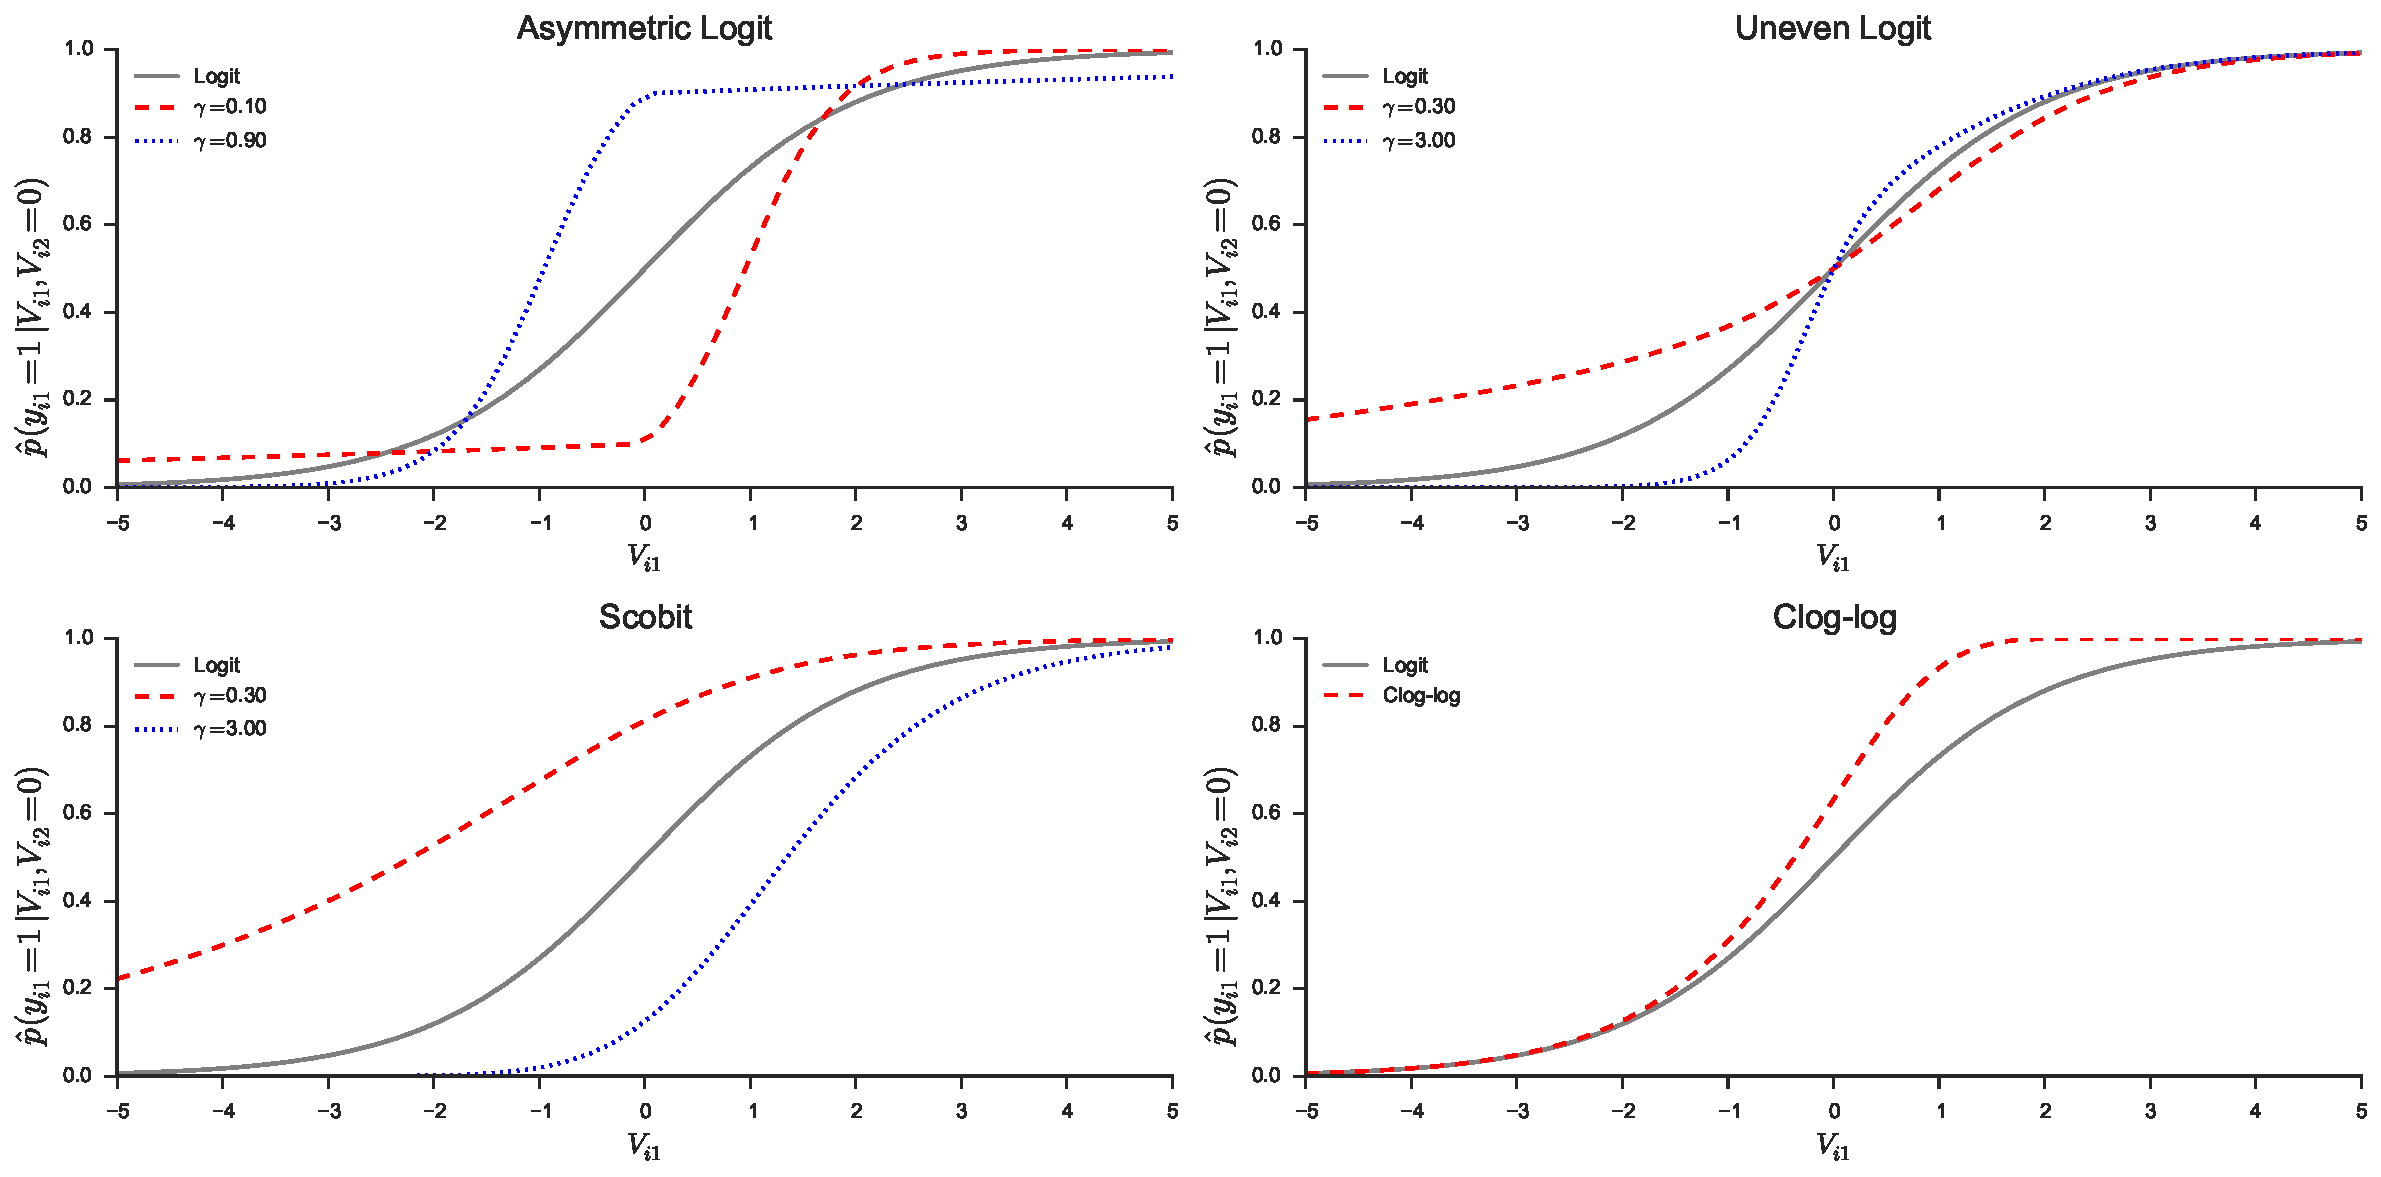
\includegraphics[width=\textwidth]{chapter3/images/Fig2_600dpi}
\caption{Binary, Asymmetric Choice Models}
\label{fig:asym_models}
\end{figure}

In the next Section, we will describe the estimation techniques used in this chapter for the logit-type models given by Equation \ref{eq:logit_type_models}. Section \ref{sec:empirical_applications} will then present the empirical applications of our logit-type models and compare them to the standard multinomial logit model, using the four example models derived in this section. Section \ref{sec:extensions} will discuss extensions to our work and finally Section \ref{sec:conclusion} will conclude.

\section{Estimation Techniques}
\label{sec:model_estimation}
Within transportation, maximum likelihood estimation (MLE) is the most commonly used technique for performing statistical inference on the unknown parameters in one's discrete choice model. For the logit-type models specified in Equation \ref{eq:logit_type_models}, the gradient and hessian of the unknown parameters $\theta = \left( \beta, \tau, \gamma \right)$ can be calculated in closed-form, provided that $S\left( \cdot \right)$ is twice differentiable and provided that the unknown parameters are constrained such that $S\left( \cdot \right)$ exists. The existence of the gradient and hessian permits one to use most numeric optimization methods to try and maximize the likelihood of one's model. Even if $S\left( \cdot \right)$ is not differentiable, one may still be able to make use of sub-gradient methods to perform such numerical maximization. 

Despite having closed-form gradients and hessians, the log-likelihood of one's logit-type model will (in general) not be concave in the unknown parameters $\theta$. This lack of concavity can make it difficult to calculate the MLE estimates for one's logit-type model. Nevertheless, when possible, we used standard optimization techniques that do not require tuning parameters such as the Newton-Raphson or the Broyden-Fletcher-Goldfarb-Shanno (BFGS) algorithms. In cases where standard techniques failed, we resorted to custom-coded gradient descent algorithms. To implement the aforementioned estimation methods, all calculations were carried out using the Python programming language and the NumPy, SciPy, and Pandas packages \citep{mckinney_data_2010, van_numpy_2011, jones_scipy_2014}. Moreover, we developed a Python package called PyLogit to perform MLE for the MNL model and the four asymmetric models introduced in Section \ref{sec:logit_type_models}. Our package, PyLogit, is available for public use through the Python Package Index.

\section{Empirical Applications}
\label{sec:empirical_applications}

% Describe application
This section describes our two policy applications of the asymmetric choice models developed in this chapter. These two applications were chosen because they differ in their respective emphases on the aggregate versus disaggregate predictions of the choice models. However, both applications use the same dataset and model specification. In particular, we model the travel mode choice of commuters in the San Francisco Bay Area who are making work or school tours. Our use of a common dataset and model specification allows us to consider the practical differences between the asymmetric and symmetric models based on use case, independent of differences in model inputs.

For our first application, we analyze the impact of a cordon toll in Downtown San Francisco on commute mode shares. As noted in the introduction, commute mode choices are almost always class imbalanced in the US. For instance, as shown in Table \ref{table:sample_mode_shares}, approximately 43\% of the 4,004 commute tours in our sample were conducted by driving alone while only 5\% were conducted by bicycling. In such class-imbalanced situations, it might be natural to suspect that one's choice probability function is asymmetric. We will investigate this hypothesis through statistical tests of our asymmetric choice models versus the MNL model and through each model's cross-validation performances. To evaluate the possible effects of the asymmetric choice models on policy analyses, in addition to the predictive performance of such models, we investigate the impact of cordon tolls on commute mode choice.

For our second application, we analyze the impact of using our asymmetric choice models in a travel demand management (TDM) setting. In particular, we focus on the use of individualized marketing to increase public transit ridership \citep{brog_individualized1998}. As a TDM strategy, individualized marketing targets individuals who do not currently use transit but nevertheless could be persuaded to use transit given the information and incentives being offered by the marketing campaign \citep{brog_individualized1998}. An example of one such incentive is the provision of free transit-passes for a limited time. This is the incentive used in our application. By assessing how ``switchable'' each individual is \citep{gensch_targeting_1984}, choice models such as the MNL model and the asymmetric models developed in this chapter are used to select individuals for targeting and transit-pass provision. We then compare the costs and programmatic success of using the MNL model versus our asymmetric logit-type models for target selection in an individualized marketing campaign by treating our sample of individuals as the population of individuals that a transit agency's pilot marketing program might have access to. Together, the TDM and cordon toll analyses will provide insight into the nature of the practical differences between the asymmetric logit-type models and the traditional MNL model.

%In the subsection below, we will describe the dataset used in our two applications. Following this, we will describe the procedures we used for model estimation, model testing, our cordon toll analysis, and our TDM example. Finally, we will report our results, and conclude this section with a discussion.
In the subsection below, we report the main results of our model estimation and policy analyses. Following this, we conclude the section with a discussion. Readers who are interested in a detailed description of the data, surrounding context, and methodology used to conduct this analysis can see Appendix D (see Section \ref{appendix:data_and_methods}).

\begin{table}
\centering

\caption{Sample Mode Shares}
\label{table:sample_mode_shares}

\begin{tabular}{lc}
\toprule
Travel Mode &  Mode Shares (\%) \\
\midrule
Drive Alone        &             42.8 \\
Shared Ride-2      &             15.9 \\
Shared Ride-3+     &             14.0 \\
Walk-Transit-Walk  &             10.3 \\
Drive-Transit-Walk &              \hphantom{*}1.5 \\
Walk-Transit-Drive &              \hphantom{*}1.3 \\
Walk               &              \hphantom{*}9.4 \\
Bike               &              \hphantom{*}4.6 \\
\bottomrule
\multicolumn{2}{l}{Note: Percentages do not sum to 100 due to rounding error.}
\end{tabular}

\end{table}

\subsection{Results}
\label{sec:application_results}
In this sub-section, we report the results of our model estimation efforts for the standard MNL model and the four asymmetric choice models derived in this chapter---the multinomial uneven logit, scobit, asymmetric logit, and clog-log models. The parameter estimates\footnote{As detailed in Appendix D, the parameter estimates for the shape parameters are reparameterized, and as such, are not the shape parameters described in Section \ref{sec:logit_type_models}. The reasons for the reparameterizations, as well as a precise description of them, are given in Appendix D.} are displayed in Table \ref{table:in_sample_MLE_estimation}. The asterisks that indicate statistical significance at the 95\% and 99\% confidence levels are based on the ``bias-corrected and accelerated'' (BCa) bootstrap confidence intervals of \citet{efron_introduction_1993} and \citet{diciccio_bootstrap_1996}. BCa intervals were used to assess statistical significance because our bootstrapping indicated that, at our current sample size, the sampling distributions of the MLEs for our asymmetric models had not yet converged to asymptotic normality. Since the sampling distributions of the MLEs had not converged to (approximate) asymptotic normality, the standard Wald tests based on such convergence were likely to be inaccurate \citep{jennings_judging_1986, pawitan_2000_reminder}. For full display of the 95\% and 99\% BCa intervals for each model, see Tables \ref{table:in_sample_MLE_interval_95} and \ref{table:in_sample_MLE_interval_99} in Appendix D.

Now, when interpreting the parameter estimation results displayed in Table \ref{table:in_sample_MLE_estimation}, one may wonder if the uneven logit model and asymmetric logit model are empirically identified. Indeed, for these two models, most of their shape parameters are not statistically significant at the 95\% confidence level. However, the uneven and asymmetric logit models are indeed empirically identified. As is well known in the statistics literature, if one is estimating both the shape parameters ($\gamma$) and the non-shape-parameters ($\tau$ and $\beta$) of a parametric link function (i.e. a choice probability function with parameters that control its shape), then the variance of one's estimates will be high when the shape parameters and non-shape-parameters are highly correlated \citep{stukel_generalized_1988, taylor_cost_1988, czado_orthogonalizing_1992}. As put by Czado, this variance increase is the ``cost'' of estimating the shape of the choice probability function within a particular parametric family \citep{czado_orthogonalizing_1992}. When we examined the correlation between shape ($\gamma$) and intercept parameters ($\tau$) of the uneven logit and asymmetric logit models, we found that these two sets of parameters were indeed highly correlated. This explains the non-significance of the estimated shape parameters and intercept terms. Moreover, each model's Hessian at the MLE had a small but existent curvature with respect to each model parameter, indicating that we do have empirical identification.

In addition to our parameter estimates, we also report the in-sample and out-of-sample predictive performance (i.e. the log-likelihoods) of each of the models in Tables \ref{table:in_sample_MLE_estimation}, \ref{table:mle_log_likelihood_by_mode}, and \ref{table:mle_cross_validation}. It can be seen that the asymmetric models generally had better predictive ability than the MNL model, both in-sample and out-of-sample. Finally, beyond the measures of statistical fit, we report the results of our applications on cordon pricing and individualized marketing for a public transportation TDM measure.

Specifically, for the cordon toll analysis, we report the aggregate, automobile-based mode share predictions by each choice model, in relation to the different toll amounts. These aggregate predictions are shown in Figure \ref{fig:mode_shares_by_toll}. Moreover, we present a comparison of the disaggregate probability forecasts of the MNL versus the uneven logit model in Figure \ref{fig:disagg_toll_prob_predictions} to highlight the disagreement between the asymmetric models and the MNL model. The map in Figure \ref{fig:drive_transit_walk_map} further emphasizes the practical significance of the differences between the MNL model and the asymmetric choice models used in this chapter. 

Finally, for the individualized marketing application, our main results are shown in Figure \ref{fig:tdm_program_efficiencies}. Defining program efficiency as the total cost of providing the free transit-passes divided by the change in the expected number of walk-transit-walk riders, Figure \ref{fig:tdm_program_efficiencies} displays the program efficiencies that are achieved by using each of the choice models for target identification. As mentioned in the following discussion section, it is useful to have Table \ref{table:mle_log_likelihood_by_mode} to help assess the program efficiency results shown in Figure \ref{fig:tdm_program_efficiencies}. Table \ref{table:mle_log_likelihood_by_mode} decomposes the overall in-sample log-likelihoods achieved by each model into the in-sample log-likelihoods achieved on each travel mode. It allows us to compare the program efficiency results to the predictive ability of each model on specific travel modes instead of just interpreting the program efficiency results based on overall model performance. In general, all of the results mentioned above will be discussed more thoroughly in the discussion section to follow (Section \ref{sec:application_discussion}).

\subsection{Discussion}
\label{sec:application_discussion}

\subsubsection{Model Estimation and Testing}
As shown in Tables \ref{table:in_sample_MLE_estimation} and \ref{table:mle_cross_validation}, the multinomial clog-log model did not perform well relative to the MNL model. However, all of the asymmetric choice models with flexible shapes (i.e. with shape parameters) more accurately predicted the mode choice of individuals in our sample than the MNL model. In particular, there were large differences in in-sample log-likelihoods between the asymmetric choice models with flexible shapes and the MNL model. These differences range from about 132 for the asymmetric logit model to 205 for the uneven logit model. Since all three of the asymmetric choice models with shape parameters nest the MNL model, log-likelihood ratio tests were used to assess whether the differences in model fit were statistically significant. Table \ref{table:in_sample_MLE_estimation} shows that all three of the asymmetric, flexible shape models had log-likelihood ratio statistics that were significant at the 0.01 alpha-level. This suggests that the MNL model is inappropriate for this dataset, relative to the flexible, asymmetric choice models used in this chapter. Moreover, the greater predictive ability of the uneven logit, the asymmetric logit, and the scobit model was not limited to just the in-sample predictions. The out-of-sample predictions in Table \ref{table:mle_cross_validation} showed exactly the same trends indicated by the in-sample results. Here, the differences in the average out-of-sample log-likelihood during cross-validation ranged from approximately 12 for the asymmetric logit to 20 for the uneven logit. Given that the testing sets in each fold of the cross-validation are about one-tenth the size of the overall dataset, these results are consistent with the in-sample results. This indicates that the greater predictive ability of the flexible, asymmetric choice models as compared to the MNL are real and not due to over-fitting.

% Report in-sample results
\begin{landscape}
\begin{table}
\centering

\caption{MLE Parameter Estimation Results}
\label{table:in_sample_MLE_estimation}

\begin{tabular}{K{0.275\linewidth}rrrrr}
\toprule
{}
Variables & \multicolumn{1}{c}{Standard Logit} & \multicolumn{1}{c}{Uneven Logit} & \multicolumn{1}{c}{Scobit} & \multicolumn{1}{c}{Asymmetric Logit} & \multicolumn{1}{c}{Clog-log} \tabularnewline
\midrule

\multicolumn{6}{l}{Alternative Specific Constants}\\
\quad Shared Ride: 2 & -1.010*\hphantom{*} & -0.806\hphantom{*}\hphantom{*} & -0.280\hphantom{*}\hphantom{*} & -1.242** & 0.969*\hphantom{*}\\
\quad Shared Ride: 3+ & 3.462** & 0.443\hphantom{*}\hphantom{*} & 2.596** & -0.724\hphantom{*}\hphantom{*} & 6.316*\hphantom{*}\\
\quad Walk-Transit-Walk & -0.392\hphantom{*}\hphantom{*} & 0.350\hphantom{*}\hphantom{*} & 11.524*\hphantom{*} & 0.490\hphantom{*}\hphantom{*} & -1.741**\\
\quad Drive-Transit-Walk & -2.622** & -3.002** & 4.388\hphantom{*}\hphantom{*} & 0.443\hphantom{*}\hphantom{*} & -4.001**\\
\quad Walk-Transit-Drive & -2.977** & -3.686** & 2.566\hphantom{*}\hphantom{*} & 0.451\hphantom{*}\hphantom{*} & -4.345**\\
\quad Walk & 1.554** & 1.626** & 0.156\hphantom{*}\hphantom{*} & 0.852** & -0.117\hphantom{*}\hphantom{*}\\
\quad Bike & -1.106** & -0.957** & -2.669** & 0.211*\hphantom{*} & -2.903**\\

\multicolumn{6}{l}{Travel Time, units:min}\\
\quad All Auto Modes & -0.076** & -4.376e-06** & -0.046** & -0.042** & -0.078**\\
\quad All Transit Modes & -0.027** & -0.364** & -0.003** & -0.016** & -0.026**\\

\multicolumn{6}{l}{Travel Cost}\\
\quad Units:\$ All Transit Modes & -0.127** & -1.718** & -0.015** & -0.080** & -0.210**\\
\quad Units:\$/mi Drive Alone & -5.061** & -3.718e-04** & -4.701** & -2.465*\hphantom{*} & -10.955**\\
\quad Units:\$/mi SharedRide-2 & -20.319** & -0.001** & -11.941** & -7.859** & -47.736*\hphantom{*}\\
\quad Units:\$/mi SharedRide-3+ & -90.922** & -0.002** & -32.494** & -16.531** & -141.947*\hphantom{*}\\

\multicolumn{6}{l}{Travel Distance, units:mi}\\
\quad Walk & -1.027** & -0.852** & -2.090** & -0.444** & -0.982**\\
\quad Bike & -0.287** & -0.211** & -0.465** & -0.164** & -0.263**\\

\multicolumn{6}{l}{Systematic Heterogeneity}\\
\quad Autos per licensed drivers (All Auto Modes) & 1.213** & 6.204e-05** & 0.597** & 0.452** & 0.764**\\
\quad Cross-Bay Tour (Shared Ride 2 \& 3+) & 0.928** & 7.841e-05** & 0.906** & 0.549** & 1.707**\\
\quad Household Size (Shared Ride 2 \& 3+) & 0.114*\hphantom{*} & 9.474e-06** & 0.074** & 0.053** & 0.073\hphantom{*}\hphantom{*}\\
\quad Number of Kids in Household (Shared Ride 2 \& 3+) & 0.687** & 3.587e-05** & 0.327** & 0.248** & 0.682**\\

\multicolumn{6}{l}{Shape Parameters}\\
\quad Drive Alone & \_\hphantom{*}\hphantom{*} & 9.716\hphantom{*}\hphantom{*} & 0.503** & \_\hphantom{*}\hphantom{*} & \_\hphantom{*}\hphantom{*}\\
\quad Shared Ride: 2 & \_\hphantom{*}\hphantom{*} & 10.000\hphantom{*}\hphantom{*} & 0.804** & 2.009** & \_\hphantom{*}\hphantom{*}\\
\quad Shared Ride: 3+ & \_\hphantom{*}\hphantom{*} & 10.190\hphantom{*}\hphantom{*} & 0.987** & 2.806\hphantom{*}\hphantom{*} & \_\hphantom{*}\hphantom{*}\\
\quad Walk-Transit-Walk & \_\hphantom{*}\hphantom{*} & -2.469\hphantom{*}\hphantom{*} & 2.917** & -1.342\hphantom{*}\hphantom{*} & \_\hphantom{*}\hphantom{*}\\
\quad Drive-Transit-Walk & \_\hphantom{*}\hphantom{*} & -2.820\hphantom{*}\hphantom{*} & 2.565*\hphantom{*} & -3.584\hphantom{*}\hphantom{*} & \_\hphantom{*}\hphantom{*}\\
\quad Walk-Transit-Drive & \_\hphantom{*}\hphantom{*} & -2.935\hphantom{*}\hphantom{*} & 2.434*\hphantom{*} & -3.953*\hphantom{*} & \_\hphantom{*}\hphantom{*}\\
\quad Walk & \_\hphantom{*}\hphantom{*} & 0.146\hphantom{*}\hphantom{*} & -0.811*\hphantom{*} & -0.958\hphantom{*}\hphantom{*} & \_\hphantom{*}\hphantom{*}\\
\quad Bicycle & \_\hphantom{*}\hphantom{*} & 0.279\hphantom{*}\hphantom{*} & -0.662\hphantom{*}\hphantom{*} & -1.632\hphantom{*}\hphantom{*} & \_\hphantom{*}\hphantom{*}\\


\multicolumn{6}{c}{}\tabularnewline

Log-Likelihood Ratio Stat. & \_\hphantom{*}\hphantom{*} & 410.148** & 341.273** & 264.828** & \_\hphantom{*}\hphantom{*}\\

Log-Likelihood & -5,073.428 & -4,868.354 & -4,902.791 & -4,941.014 & -5,116.066\\

\bottomrule
\multicolumn{6}{l}{Note: * means $\textrm{p-value} < 0.05$ and ** means $\textrm{p-value} < 0.01$.}
\end{tabular}

\end{table}
\end{landscape}

% Report the in-sample log-likelihoods by mode
\begin{table}
\centering

\caption{MLE In-Sample Log-likelihoods by Travel Mode and by Model}
\label{table:mle_log_likelihood_by_mode}

\begin{tabular}{lrrrrr}
\toprule
{} &  Standard Logit &  Uneven Logit &    Scobit &  Asymmetric Logit &  Clog-log \\
\midrule
Drive Alone        &      -1,084.14 &    -1,045.70 &  -1,040.07 &        -1,045.04 &  -1,092.69 \\
Shared Ride: 2     &      -1,183.66 &    -1,138.00 &  -1,144.92 &        -1,151.32 &  -1,196.55 \\
Shared Ride: 3+    &        -905.80 &      -826.15 &    -844.65 &          -847.57 &    -926.98 \\
Walk-Transit-Walk  &        -572.69 &      -566.87 &    -569.84 &          -572.85 &    -581.04 \\
Drive-Transit-Walk &        -184.99 &      -177.76 &    -177.20 &          -182.35 &    -185.73 \\
Walk-Transit-Drive &        -176.93 &      -167.30 &    -167.32 &          -176.54 &    -175.32 \\
Walk               &        -520.07 &      -502.27 &    -515.38 &          -519.54 &    -513.11 \\
Bike               &        -445.16 &      -444.30 &    -443.42 &          -445.80 &    -444.65 \\
\tabularnewline
Total              &       -5,073.43 &     -4,868.35 & -4,902.79 &         -4,941.01 & -5,116.07 \\
\bottomrule
\end{tabular}

\end{table}

% Report out-of-sample results
\begin{table}
\centering

\caption{MLE Average Out-of-Sample Log-likelihood During 10-fold Cross-Validation}
\label{table:mle_cross_validation}

\begin{tabular}{lc}
\toprule
Model &  Log-Likelihood \\
\midrule
Uneven Logit     &         -490.12 \\
Scobit           &         -494.04 \\
Asymmetric Logit &         -498.44 \\
Standard Logit   &         -510.28 \\
Clog-log         &         -514.63 \\
\bottomrule
\end{tabular}


\end{table}

% Report policy analysis results
\begin{figure}
\centering
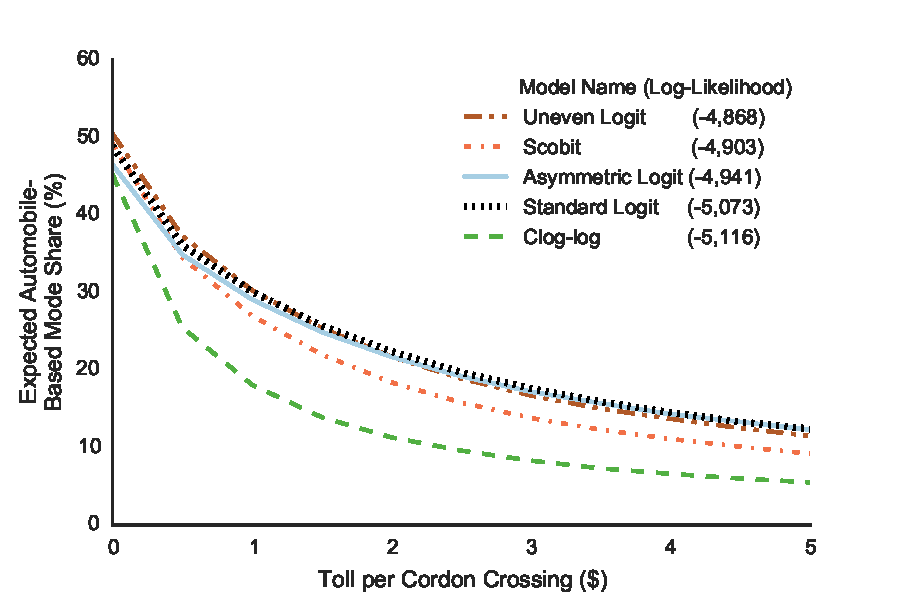
\includegraphics[width=\textwidth]{chapter3/images/Fig4}
\caption{Automobile-Based Mode Shares by Model and by Cordon Toll Amount}
\label{fig:mode_shares_by_toll}
\end{figure}

\begin{figure}
\centering
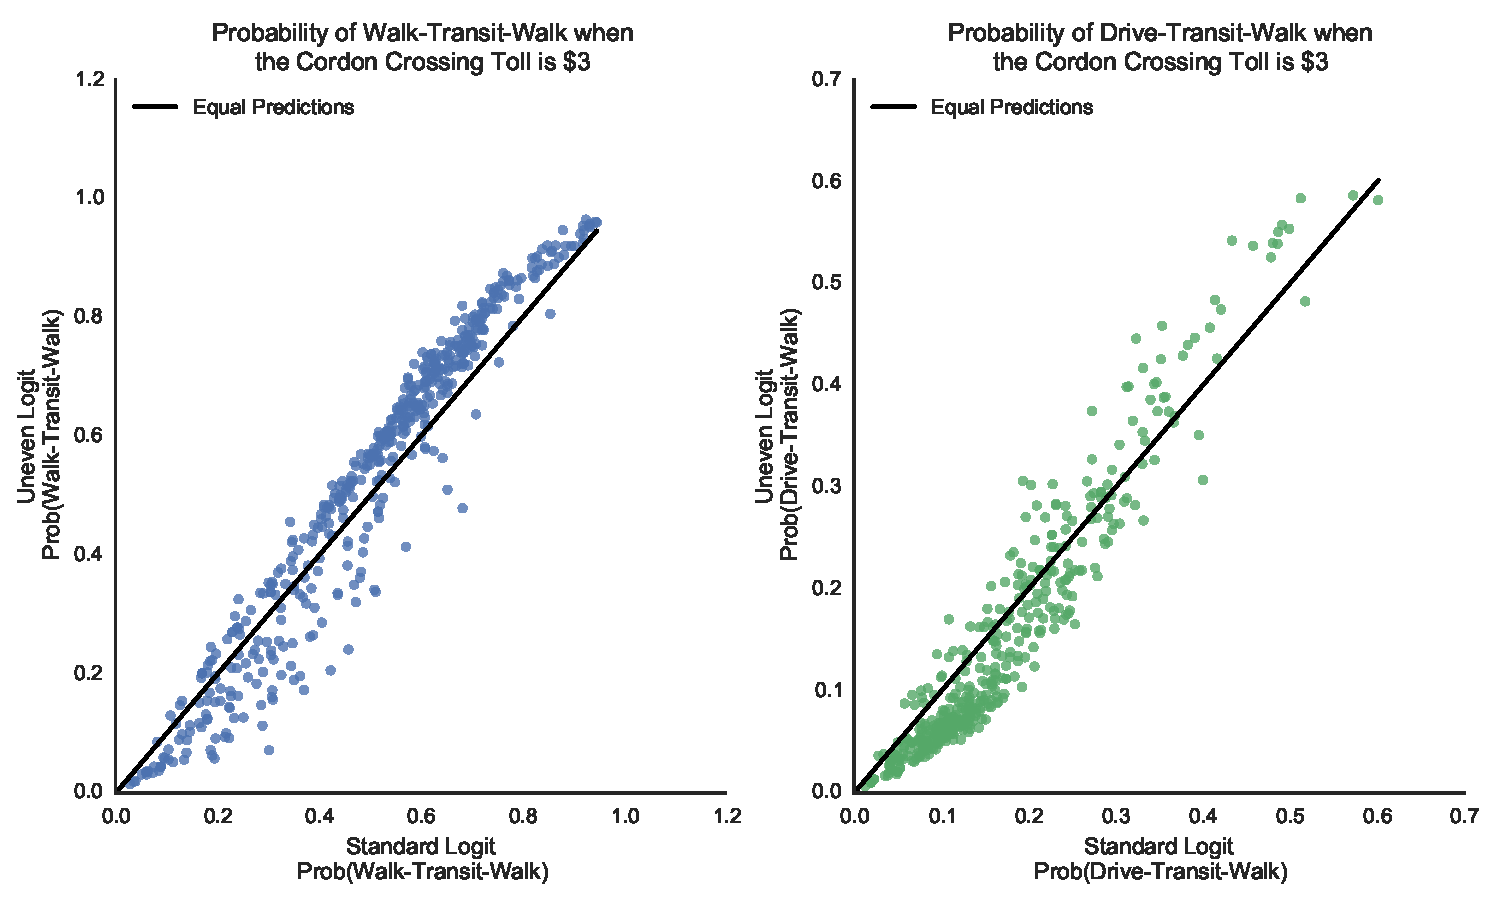
\includegraphics[width=\textwidth]{chapter3/images/Fig5}
\caption{Disaggregate Probability Predictions for Walk-Transit-Walk and Drive-Transit-Walk for the Uneven Logit and the MNL Models}
\label{fig:disagg_toll_prob_predictions}
\end{figure}

\begin{figure}
\centering
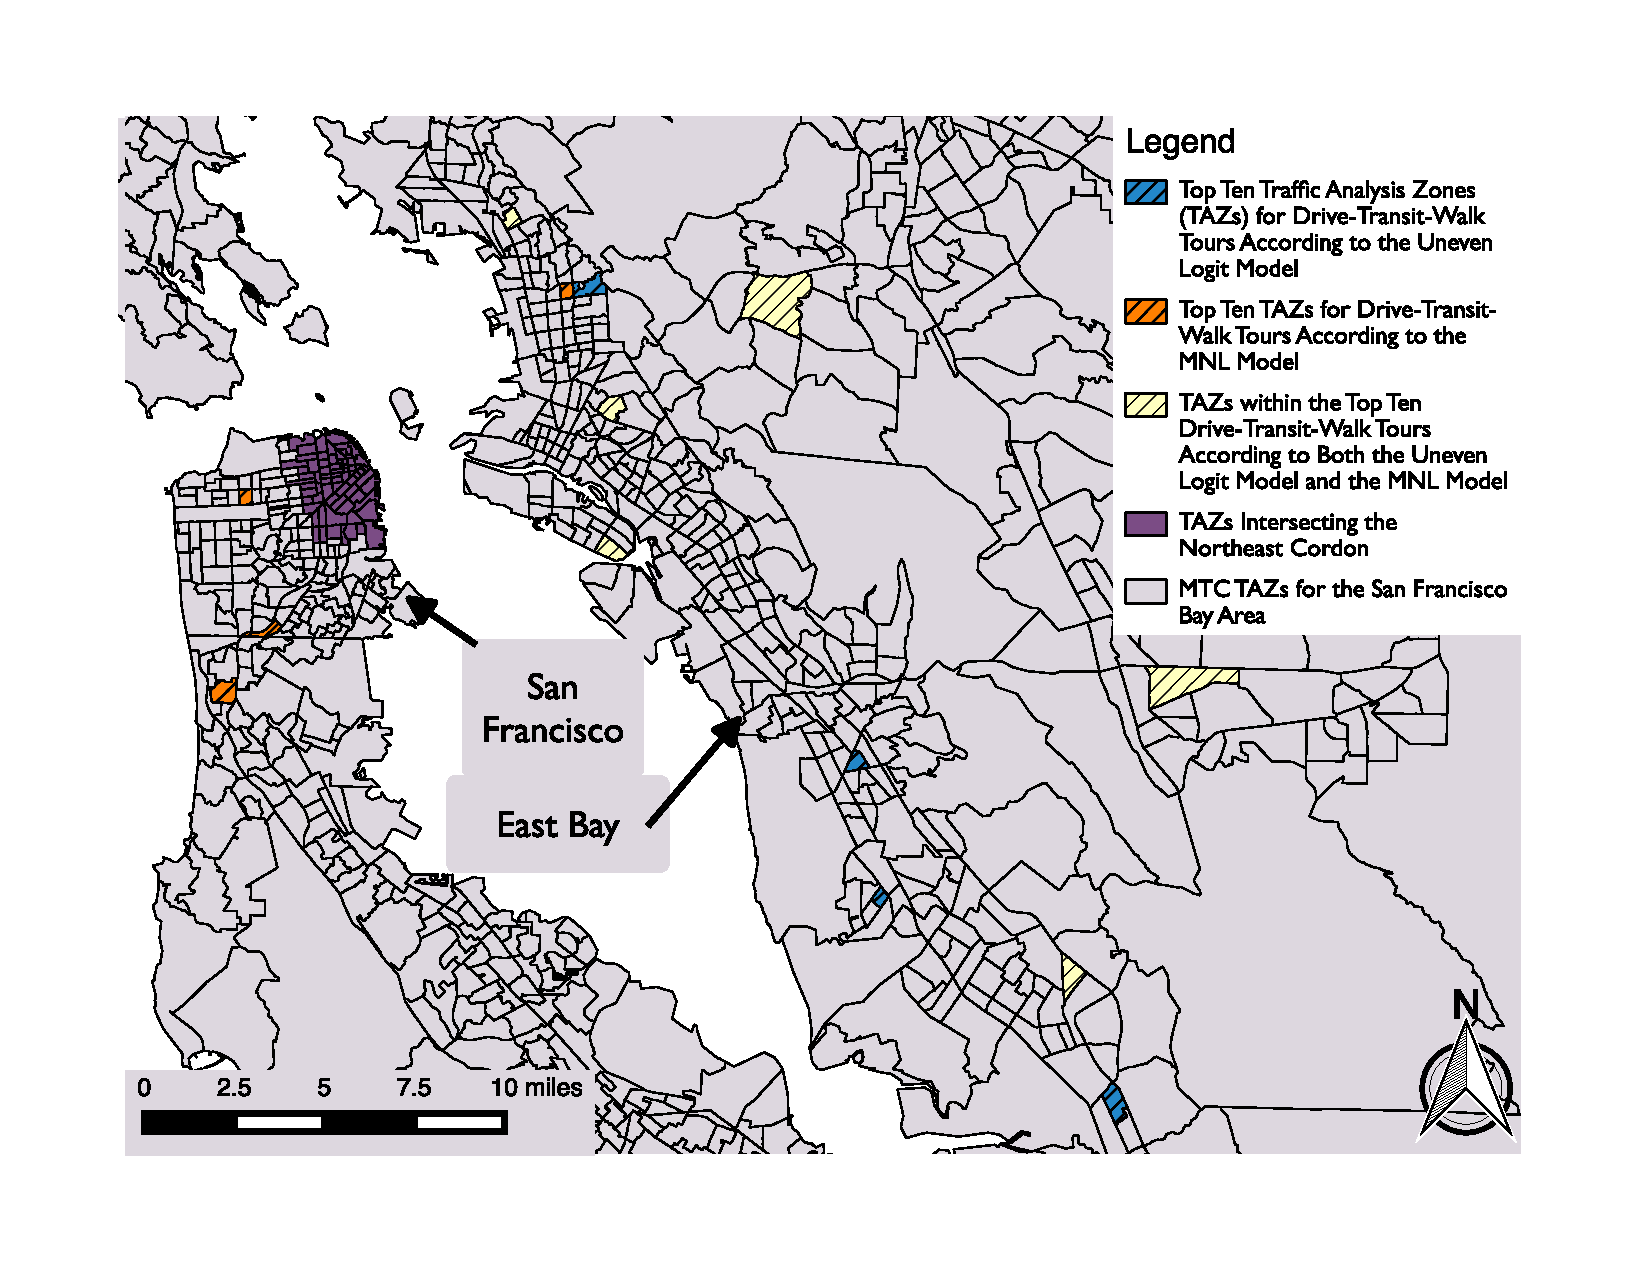
\includegraphics[width=\textwidth]{chapter3/images/new_Fig_6}
\caption{Top Ten Traffic Analysis Zones Producing Drive-Transit-Tours \newline According to the Uneven Logit and MNL Model at \$3 per Cordon Crossing}
\label{fig:drive_transit_walk_map}
\end{figure}

\begin{figure}
\centering
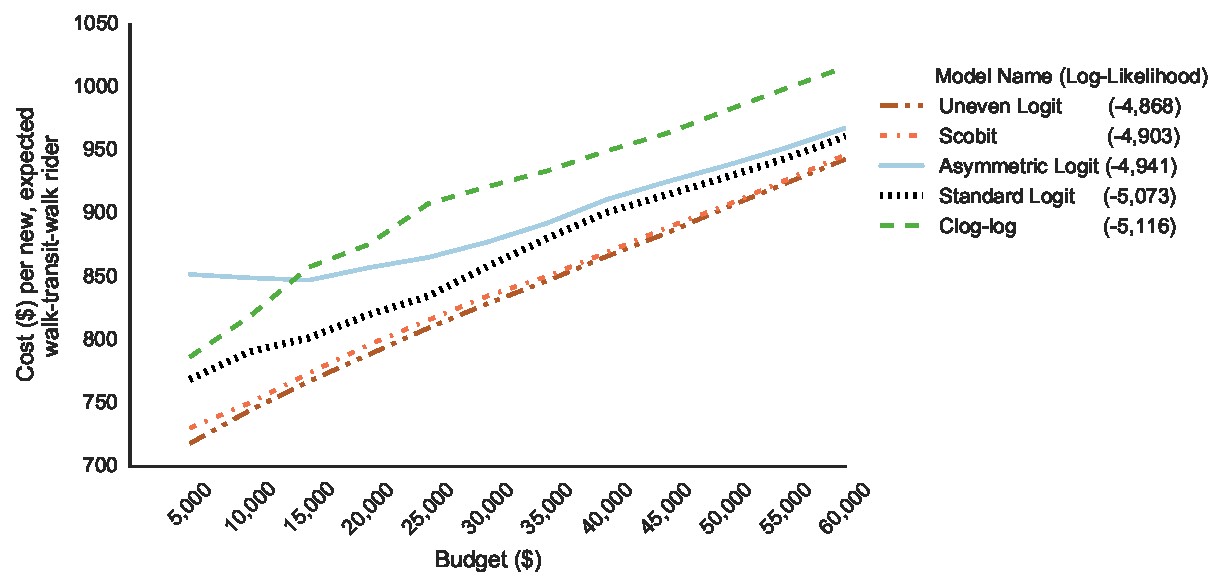
\includegraphics[width=\textwidth]{chapter3/images/Fig8}
\caption{Total Individualized Marketing Costs Per New, Expected Walk-Transit-Walk Rider by Model}
\label{fig:tdm_program_efficiencies}
\end{figure}

\subsubsection{Cordon Toll Analysis}
In addition to judging whether the improvements offered by one model over another are ``statistically significant,'' it is important to assess whether such improvements are ``practically significant.'' One way we assessed the practical impacts of the asymmetric choice models derived in this chapter was to conduct an analysis of the effects of a congestion cordon toll\footnote{From economic theory, if a set of alternatives are perfect substitutes for one another, then the marginal dis-utility of cost should be constant across the alternatives since the goods are exactly the same. Because our estimated cost-coefficients for the Drive Alone, SharedRide-2, and SharedRide-3+ modes show large differences from one another, we have reason to believe that these three automobile alternatives are not perfect substitutes for one another, even after controlling for our study's explanatory variables. Accordingly, we conclude that there is some set of unobserved variables that still differentiates the three modes from each other and which interacts with the cost variable to influence an individual's cost-sensitivity for each mode. While recognizing this issue, we are not sure what these unobserved variables might be, and even if we did have thoughts about what these unobserved variables might be, we are not in a position to collect data on these features. As a result, both our cordon toll and TDM analysis are therefore conditional on the following \textit{ceteris paribus} assumption: that the interaction effects between cost and these unobserved variables remain as they currently are, despite external changes to the cost of the various automobile-based modes. Thanks to an anonymous reviewer for raising this point.} in Downtown San Francisco. 

At the most basic level, we compare the MNL model and the asymmetric choice models on the basis of their aggregate, predicted mode shares for automobile-based modes (drive alone, shared ride with two passengers, and shared ride with three or more passengers) under various cordon toll charges. Given that the purpose of the congestion toll is to reduce the use of automobile-based modes at peak commute times, large differences in predicted mode share for automobile-based modes would have great ramifications for support and expectations of the congestion tolling scheme. As shown in Figure \ref{fig:mode_shares_by_toll}, the aggregate mode share predictions for the automobile based modes, for tours that cross the cordon, follows the same general trend for both the MNL and the flexible, asymmetric choice models. Moreover, the differences in the predicted mode shares are minimal. Compared to the flexible, asymmetric models, the MNL model overestimates the mode share of automobile-based modes by 1-3.8\% at the San Francisco County Transportation Authority's proposed toll of \$3 per cordon crossing, depending on which model is being examined. However, the MNL and flexible asymmetric models all predicted overall decreases of approximately 31-35\% in automobile based mode shares from a \$0 toll to a \$3 toll. In light of the overall predicted mode share changes, the differences between models seems mostly inconsequential from a general planning perspective.

Beyond the basic question of how the aggregate, automobile-based mode shares will change as a result of tolling, a host of disaggregate outputs from mode choice models may be useful for transportation agencies implementing the congestion toll. In particular, to support individuals making their commute trips under the tolling scheme, transportation agencies should make switching to more sustainable modes (such as public transit) as easy and safe as possible. For example, at transit stations where one expects the average number of drive-transit-walk commuters to increase, and where parking capacity is nearly full at peak hours, transit agencies might want to increase parking capacity so that 'park-and-ride' trips can be more readily accommodated. However, such actions require knowledge of which transit stations have catchment areas that are going to see large increases in their drive-transit-walk mode shares. 

To be accurate, these station-level determinations require accurate predictions of the disaggregate drive-transit-walk probabilities for individuals. In our application, we find substantive disagreements between the MNL model and the flexible, asymmetric choice models. For example, Figure \ref{fig:disagg_toll_prob_predictions} shows the predicted probabilities of walk-transit-walk and drive-transit-walk with a cordon toll of \$3 according to both the MNL model and the uneven logit model for the 4,004 tours in our sample. As can be seen, many of these predicted probabilities disagree. These disagreements are not just an artifact of the \$3 toll, but they exist at every tolling amount we tested, including the base case scenario with no toll. The substantive impact of these individual-level disagreements is that practitioners deciding where to install pedestrian improvements and increase parking capacity based on the MNL model might make misguided decisions: installing infrastructure where it is not needed, or failing to install infrastructure where it is needed. For instance, Figure \ref{fig:drive_transit_walk_map} shows the ten traffic-analysis-zones producing the greatest expected numbers of drive-transit-walk tours into the cordon area for the MNL model and the Uneven Logit model at \$3 per cordon crossing. As shown by the map, the MNL model under-predicts the amount of drive-transit-walk trips from the East Bay into the cordon area, relative to the uneven logit model. Practitioners using the MNL model as opposed to the uneven logit model might then incorrectly underestimate the need for increased parking capacity at BART stations in the East Bay, thereby hampering the success of the congestion pricing effort.

\subsubsection{TDM Analysis---Individualized Marketing}
Continuing with the emphasis on disaggregate model differences, this subsection discusses the practical differences for an individualized marketing campaign for TDM. Here, we assume the role of an agency interested in maximizing the increase in the expected number of walk-transit-walk riders per dollars expended. As such, the differences that we are concerned with in this application result from selecting individuals for targeting using each of the choice models being compared in this chapter. To the extent that the different models select different individuals, the costs of providing the transit-passes will differ, and the change in the expected number of new walk-transit-walk commuters will differ.

Using the uneven logit model to estimate the ``true'' change in the expected number of new walk-transit-walk commuters (since the uneven logit model had the highest in-sample and out-of-sample log-likelihoods---see Tables \ref{table:in_sample_MLE_estimation} and \ref{table:mle_cross_validation}), Figure \ref{fig:tdm_program_efficiencies} shows the ratio of the ``program efficiencies'' achieved by each model, for a range of budgets for purchasing the transit passes. From this Figure, a few insights can be gleaned. 

First, when only a small proportion of the sample can be targeted (i.e. when the budget is low), the scobit and uneven logit models make the best uses of money relative to the MNL model. For instance, with a \$5,000 budget, the MNL spends \$770 per new expected walk-transit-walk passenger, while the scobit and uneven logit models spend \$731 and \$719, respectively. If the number of individuals in the marketing program increases while the proportion that is targeted remains the same, such differences in program efficiency will lead to large differences in the number of new walk-transit-walk riders that are attracted using each model's targeting list. Second, as the budget increases and the proportion of individuals that can be targeted increases, the differences between the program efficiencies of each model are greatly reduced. This is to be expected. At the limit, there will be a large enough budget to select all individuals for targeting, thus the program costs and the ``true'' increase in the expected number of walk-transit-walk passengers will be equal across models. Lastly, the ranking of program efficiencies across models depended not on the overall predictive ability of one's multinomial model but mostly on the predictive ability of one's model for the travel mode of interest (walk-transit-walk in this case). For instance, since the asymmetric logit model's in-sample and out-of-sample log-likelihoods are higher than those of the MNL model (see Tables \ref{table:in_sample_MLE_estimation} and \ref{table:mle_cross_validation}), one would expect the asymmetric logit model to make better targeting selections than the MNL model. However, when one looks at the log-likelihoods of each model for just the walk-transit-walk mode (shown in Table \ref{table:mle_log_likelihood_by_mode}), we can see that the asymmetric logit model is actually a worse predictor of the walk-transit-walk mode than the MNL model, even though it is has a higher log-likelihood overall. It's program efficiency is therefore worse than that of the MNL model. Another seemingly anomalous fact is that when the budget is low, the clog-log model is able to better target individuals than the asymmetric logit model. This merely reflects the fact that for this sample and relative to the asymmetric logit model, the clog-log model is better able to find the small handful of individuals providing the highest increase in their probability of commuting via walk-transit-walk per dollar spent. However, as the budget increases and the number of individuals that is to be targeted increases, the ranking of program efficiencies return to the predictable state of mimicking the in-sample, log-likelihood rankings for the walk-transit-walk mode.

Overall, for our individualized marketing application, we find that when resources are limited (i.e. when only a small percentage of one's population can be targeted for marketing), the use of the MNL model can be inefficient as compared to the asymmetric choice models such as the uneven logit and scobit models. In our example, such inefficiencies cost the MNL an additional \$51 per new expected walk-transit-walk rider when compared to the uneven logit model. As the budget for the marketing campaign and the percentage of individuals that could be targeted increased, the disaggregate predictive abilities of each model became less important, and as with the cordon toll application, the practical differences between models became minimal.


\subsection{Summary}
Through our analysis of the commute mode choices of San Francisco Bay Area residents, we found that the three asymmetric choice models with flexible shapes (i.e. those with shape parameters) had much better predictive ability (overall) than the standard MNL model. This result was observed in both in-sample and out-of-sample log-likelihoods. Moreover, these results were corroborated through our log-likelihood ratio test results. All of our flexible asymmetric models had log-likelihoods that were higher than the MNL model, at statistically significant levels.

With regard to practically significant differences, we find that the MNL model and the flexible, asymmetric choice models yield similar \textit{aggregate} inferences in our cordon toll analysis. In particular, results concerning the aggregate mode shares of automobile-based modes at different tolling levels are virtually equal across the different models. The practical differences between the MNL and flexible, asymmetric models comes from the \textit{disaggregate} predictions of the various models for each individual, and the fact that the predictions for some modes may differ greatly. Specifically, the predictions for walk-transit-walk and drive-transit-walk differ greatly between the MNL model and the flexible, asymmetric models in our example. 

The practical significance of these differences for our cordon toll application is that discordant inferences are obtained regarding where transit-serving parking supply should be increased. The MNL model suggests that transit-serving parking should be added in San Francisco itself, whereas the asymmetric models imply that the most important places to increase transit-serving parking supply are all in the East Bay. Due to the higher land values in San Francisco and a lower supply of land to devote to parking, the use of the MNL model instead of its better performing, asymmetric counterparts would lead transportation agencies to misguidedly spend much more money providing parking in San Francisco, when the East Bay is likely in greater need for transit-serving parking under a congestion tolling scheme.

For our TDM application, the practical significance of our models is that the asymmetric choice models that predict the walk-transit-walk mode better than the MNL model can better guide investment of the money that is available for individualized marketing of public transit. Specifically, we found that in our example, when the budget for providing free transit passes was low (\$5,000), the cost of acquiring each new walk-transit-walk rider could be reduced by approximately \$50 and \$40, respectively, by using the uneven logit model and the scobit model for target selection instead of the MNL model. Conversely, as the budget and the percentage of individuals who could be targeted increased, the differences in the disaggregate predictions of the models mattered less and less for target selection and the resulting efficiency of the marketing campaign. This further underscores the fact that the practical usefulness of  asymmetric choice models appear to be highest when accurate, disaggregate predictions are needed.

Moving onto the remaining two sections of this chapter, we will now transition from discussing our specific applications to looking more broadly at how our work on asymmetric, closed-form, finite-parameter models of multinomial choice can be extended. Then in Section \ref{sec:conclusion}, we will conclude by summarizing the theoretical contributions of this chapter, highlighting our empirical results, and raising key research questions from this work that should interest academic scholars and professional analysts.

\section{Extensions}
\label{sec:extensions}
Thus far, all of the individual models and results that have been shown in this chapter have been based on the general formulation of logit-type models given by Equation \ref{eq:logit_type_models}. Despite restricting ourselves to that proposed class of models, at least six extensions or future research directions are immediately apparent. In particular, these ideas for future work can be categorized as either (1) direct extensions of the logit-type models developed in this chapter, (2) applications of this chapter's ideas to other models, or (3) investigations of the statistical properties of logit-type models. In the following paragraphs we will detail each of the extensions and future research directions that comprise these categories.

Firstly, the logit-type models given in Equation \ref{eq:logit_type_models} can avoid the symmetry property of standard MNL models, but because they share the same functional form as the MNL model, they retain other undesired properties such as I.I.A. Accordingly, many of the motivations behind existing extensions to the MNL model remain equally applicable to our proposed class of logit-type models. Here we highlight three such extensions. First, models such as the ``Heteroskedastic Logit Model'' \citep{steckel_heterogeneous_1988, recker_discrete_1995, bhat_heteroscedastic_1995} allow the scale parameter to vary across observations, and this effectively allows the shape of the resulting choice probability function to vary across observations. An analogous extension to logit-type models would be to allow $\gamma_j$ to vary across individuals, such as by parametrizing it as a function of $x_{ij}$. Such parametrizations have been successfully used in a transportation context to improve the fit of binary scobit models \citep{zhang_scobit-based_2010, wu_analysis_2012}, but this type of extension can be more generally applied to any logit-type model that has shape parameters. Second, the wider class of ``multivariate extreme value''\footnote{This class was originally referred to as ``generalized extreme value'' (GEV) models \citep{mcfadden_econometric_1980}. The name multivariate extreme value was adopted to avoid confusion with the pre-existing generalized extreme value distribution \citep{jenkinson_frequency_1955}.} models (such as the nested and cross-nested logit) generalizes the MNL model, capturing arbitrary correlations between the utilities of an individual's various alternatives while still maintaining a closed-form expression \citep{train_discrete_2009}. Logit-type models would benefit from similar extensions. As mentioned in Section \ref{sec:logit_type_literature_relation}, one way to extend logit-type models to account for correlation between the utilities of one's alternatives is to specify various ``aggregation functions'' as described by Mattsson et al. (\citeyear{mattsson_extreme_2014}) in conjunction with $w_{ij} = \exp \left[ \tau_j + S \left( V_{ij}, \gamma_j \right) \right]$. Lastly, MNL models have been extended using various ``mixing distributions'' to account for taste heterogeneity in their parameters and to provide realistic substitution and correlation patterns between alternatives \citep{revelt_mixed_1998}. These mixed logit approaches use a MNL ``kernel'' and allow the $\beta$ coefficients to be randomly distributed throughout the population. Similar mixing strategies could be followed whereby one used a logit-type model as the kernel and a continuous mixing distribution of $\beta$s in the model. If using a discrete mixing distribution, i.e. a Latent Class Choice Model (LCCM), an analogous procedure is to use a logit-type model for the class-specific choice model. Such mixing procedures would allow for much greater flexibility and behavioral realism in our proposed logit-type models.

Beyond the direct extensions already mentioned, future research directions include applying the techniques and concerns of this chapter to other choice models. Two such research directions seem immediately promising. First, as noted at the end of the last paragraph, one can consider using a logit-type model as the class-specific choice model in a LCCM. However, this still begs the question of what choice model should be used as the class-membership model. It is not clear that one would necessarily want the class-membership model to have the symmetry property described in the introduction, so it would be interesting to look at the effects of using an asymmetric, logit-type model as the class-membership model in one's LCCM. There could be large policy impacts from such a change. For instance, imagine one is interested in growing the market share of a desired market segment, such as a latent class of individuals with a predisposition towards using non-motorized modes of transportation. If that market segment is forecast to grow much more slowly when using an asymmetric model for the class membership probabilities as opposed to a MNL, and the asymmetric model fits one's data better, then policy-makers may need to take more aggressive measures to increase the market shares of the desired class. Secondly, the logit-type models developed in this chapter were based on the desire to make the MNL model asymmetric. However, as stated above, this logit-based lineage leads to the inheritance of the other undesired properties of the logit model such as I.I.A. It would be interesting to instead try and make other, non-logit-based, choice models asymmetric. For instance, the Exponomial Choice model is not based on the logit model, yet it shares some of the attractive properties of the logit model. In particular, it has a closed-form probability equation, it has a log-likelihood that is concave with respect to the $\beta$s to be estimated, and it does not have the I.I.A. property \citep{alptekinoglu_exponomial_2016}. However, it is a symmetric choice probability function\footnote{This assertion is made based on plotting the choice probabilities for the binary exponomial choice model.}. It would be quite interesting to develop an asymmetric analogue to the Exponomial Choice model, as such a model would avoid both the I.I.A. property and the symmetry property.

Finally, there are a number of statistical questions regarding logit-type models that remain to be investigated. One point, raised by a referee, is that one does not know (a-priori) which logit-type model will be best for one's application. Therefore, one essentially has to try them all. As a result of this fact, it would be useful to study the characteristics of the best performing transformation functions $S \left( \cdot \right)$ in relation to the intrinsic characteristics of one's data. If such research leads to a greater understanding of how to specify one's $S \left( \cdot \right)$ functions, then one may be able to save researchers a fair amount of computational effort. More generally, it would be worthwhile to perform simulation studies to gain insight into the conditions under which asymmetric models perform better than symmetric ones and into the conditions that favor various types of asymmetry. In the meantime, the situation with logit-type models is analogous to the situation that is already faced in research, where (for instance) a researcher may not be certain (a-priori) of which plausible nesting or cross-nesting structure will be better in one's application.

Another statistical question is what is the best way to estimate one's logit-type model? As was noted in Section \ref{sec:model_estimation}, MLE was sometimes difficult for the four logit-type models derived in this chapter. One response is to use Bayesian techniques to estimate the logit-type models since these techniques do not require maximization of an objective function. However, Bayesian estimation techniques can potentially lead to long estimation times, depending on one's model, dataset, and specific estimation method. It would be useful to investigate the properties of Bayesian and other estimation techniques on logit-type models. For instance, it has already been shown that maximum entropy estimation \citep{donoso_maximum_2011} may be a better estimation technique than MLE for nested logit models. Further research should be done with logit-type models to investigate the implications, the possible equivalences, and the relative merits and drawbacks of various estimation techniques such as bayesian inference, maximum entropy, method of moments, minimum chi-square estimation \citep{berkson_minimum_1980}, etc.

Lastly, it may be interesting to investigate the differences between this chapter's various asymmetric models by studying the models' influence functions and influential observations. The primary questions to answer would be whether the various estimated models are highly influenced by differing observations, or whether the different models are differentially suited for different types of outlying or high-leverage observations. Such investigations may lead to more data-driven methods for constructing the asymmetric, logit-type model that is best for one's application. 

\section{Conclusion}
\label{sec:conclusion}

% Restate the main problem
% Restate one’s solution to the main problem
In this chapter's introduction, we called attention to a symmetry property of common discrete choice models such as the MNL model and the simple probit model. Arguing that it is often undesirable for one's discrete choice model to a-priori be symmetric, we introduced a class of ``logit-type'' models that allow one to specify choice models of varying shapes and asymmetries, without entailing restrictions on the signs or magnitudes of the indices, $V_{ij}$.  Essentially, logit-type models replace the index, $V_{ij} = x_{ij} \beta$ in the MNL model with functions, $S \left( \cdot \right)$, that depend on the index and a finite number of shape parameters that control the shape of the choice probability function. By ensuring that this new function is asymmetric with respect to the index $V_{ij}$, we avoid symmetry in our logit-type models.

% Emphasize one’s contributions.
Next, we showed that our proposed class of models is both a parametrization of the class of models introduced by Mattsson et al. (\citeyear{mattsson_extreme_2014}) as well as a generalization of numerous existing, asymmetric choice models from both the transportation discipline as well as statistics. This nesting of existing models was used to devise a methodology for extending numerous pre-existing models to the ``conditional'' and multinomial settings. Such extensions greatly increase the number of situations that can be modeled by existing asymmetric choice models and increase the relevance of such models to transportation researchers whom often study inherently multinomial choice contexts. As examples of the proposed method, we extended two existing models---the clog-log model and the scobit model---to the multinomial setting for the first time.

Recognizing that the existing asymmetric choice models may not always suit a researcher's needs, we proposed a method for creating new, asymmetric choice models. We break from recent trends in transportation whereby one first specifies the distribution of each alternative's utility to each individual and then derives the choice probability functions as a result. Our work takes the opposite approach of directly specifying the form of the choice probability functions, knowing that our logit-type models can be derived from innumerable distributions of the utilities. Doing so frees us to specify the choice probability functions according to the properties that we find desirable for our study. To demonstrate our proposed procedure, we derived two new choice models that generalize the MNL model: the asymmetric logit model and the uneven logit model.

To test the four new models derived in this chapter against the standard MNL model, we applied all of these models to an analysis of travel mode choice in the San Francisco Bay Area. We find that all of the asymmetric choice models with flexible shapes (i.e. those with shape parameters to be estimated from the data) were able to fit the data better according to both in-sample and out-of-sample log-likelihoods. The difference in fit, for our example, was not just statistically significant but quite dramatic---on the order of more than 200 log-likelihood points for a dataset of only 4,004 individuals with 8 alternatives. Moreover, beyond the statistical fit and predictive ability of the various models, we showed that switching to asymmetric choice models can also entail serious policy implications. When looking at the effects of a cordon toll in Downtown San Francisco, we found that relative to the flexible asymmetric choice models (which had greater predictive power), the MNL model over-predicted the number of drive-transit-walk tours coming from San Francisco. Such over-predictions would encourage transportation agencies to erroneously invest more in increasing transit-serving parking supply in San Francisco as compared to the East Bay, where all of the other asymmetric models predict high expected numbers of drive-transit-walk tours. Moreover, in our TDM application, we find that the uneven logit model and the scobit model are able to better target individuals for marketing when funding for such a campaign is limited. In particular, the uneven logit and scobit models are able to reduce the cost of acquiring each new walk-transit-walk customer by approximately \$50 to \$40 relative to the MNL model when the marketing budget is only \$5,000. These results suggest that while asymmetric models may not always outperform symmetric ones, asymmetric choice models are at least worth testing in one's analysis as they might have better statistical performance and entail substantive policy and financial implications.

% Position one’s work in larger bodies of literature, both on the specific problem and in discrete choice and statistics at large
Lastly, while this chapter presents a new class of models as well as four particular instances of this new class, many extensions to this work and future research directions remain. By direct analogy with MNL models, it will be of interest to extend logit-type models to account for arbitrary correlation structures between the various utilities of each alternative. Moreover, it will be interesting to make use of mixture formulations to incorporate taste heterogeneity and flexible patterns of substitution between alternatives. Regarding applications, further investigation remains to be done on the effect of incorporating logit-type models into other contexts (such as modeling market segmentation in LCCMs) and on the effect of incorporating asymmetry into choice models with different functional forms from the logit model (such as the Exponomial Choice model). Alongside all of the research directions mentioned above, there will of course be a need to answer statistical questions related to the proposed model-class, including questions of how best to estimate logit-type models and how one can check the appropriateness of a given function, $S \left( \cdot \right)$, for one's data.

\section*{Acknowledgements}
We thank James A. Goulet for many stimulating conversations in the beginning stages of this research. Additionally, we thank Michael Fratoni for computational assistance in the beginning of this project. Thanks go to Madeleine Sheehan and the anonymous referees for their constructive criticism of this manuscript. Any remaining errors or omissions are, of course, our own. Lastly, we thank UCCONNECT and Caltrans for funding this research effort.

\newpage
\section{Appendix A: Proofs}
\label{appendix:proofs}
Here we provide the derivation of Equation \ref{eq:cpe_loss_to_binary_prob}. It is based on Equation 16 and Equation 45 of \citet{buja_loss_2005}. Note that in all equations below, we use the notation introduced in Section \ref{sec:binary_to_multinomial}.

First, Equation 16 of \citeauthor{buja_loss_2005} states that:
\begin{equation}\tag{A1}
\label{eq:A1}
L_{2} \left( \hat{p} \left( V_{i1} \right) \right) = \int _0 ^{\hat{p}\left( V_{i1} \right)} tw\left(t\right)dt
\end{equation}
Applying the Fundamental Theorem of Calculus to Equation \ref{eq:A1}, we can write:
\begin{equation}\tag{A2}
\label{eq:A2}
\frac{d\left[ L_{2} \left( \hat{p} \left( V_{i1} \right) \right) \right]}{d\hat{p}} = \hat{p} \left( V_{i1}  \right) w \left( \hat{p} \left( V_{i1} \right) \right)
\end{equation}
At the same time, Equation 45 of \citeauthor{buja_loss_2005} states:
\begin{equation}\tag{A3}
\label{eq:A3}
1 = w \left( \hat{p} \left( V_{i1}  \right) \right) \hat{p}' \left( V_{i1}  \right)
\end{equation}
Assuming that $\hat{p}' \left( V_{i1}  \right) \neq 0$, we can rearrange Equation \ref{eq:A3} as follows:
\begin{equation}\tag{A4}
\label{eq:A4}
\frac{1}{\hat{p}' \left( V_{i1}  \right)} = w \left( \hat{p} \left( V_{i1}  \right) \right)
\end{equation}
Finally, substituting Equation \ref{eq:A4} into Equation \ref{eq:A2} yields Equation \ref{eq:cpe_loss_to_binary_prob}.

\newpage
\section{Appendix B: Further relations to existing literature}
\label{appendix:lit_relations}
In this appendix, we provide further details on the relationship between our models and those of \citet{li_multinomial_2011} and \citet{das_generalized_2014}. Additionally, for convenience, we provide a table showing how our proposed class of logit-type models subsumes previously described asymmetric models as special cases.

First, while the models based on Weibull, Rayleigh, Type II Generalized Logistic, Pareto, or Exponential distribution utilities are generalized by both our logit-type models and the single-index model of \citet{li_multinomial_2011}, our logit-type models given by Equation \ref{eq:logit_type_models} \textbf{\textit{are not}} a special case of Li's model. In particular, \citet{li_multinomial_2011} estimates a single $S \left( \cdot \right)$ for all alternatives. The transformations used in our logit-type models are allowed to differ across alternatives, based on the values of the shape parameters $\gamma _j$ for each alternative. Secondly, our chapter provides a general method to create new, closed-form, binary probability functions. The paper of \citet{li_multinomial_2011} does not. \citet{li_multinomial_2011} instead focuses on semi-parametric, binary probability functions. Finally, our work provides a method and rationale for generalizing binary probability functions to the multinomial setting, whether or not the distribution of the utilities underlying the probability function are known. The paper of \citet{li_multinomial_2011} provides no such distribution-free method for generalizing existing binary probability functions.

Next, with respect to the paper by \citet{das_generalized_2014}, our work is strictly more general. \citet{das_generalized_2014} only consider a single $S\left( \cdot \right)$ function, namely that of \citet{czado_parametric_1994}. This chapter considers general, closed-form $S\left( \cdot \right)$ functions. As noted in Section \ref{sec:logit_type_literature_relation} and as shown below in Table \ref{table:logit-type-special-cases}, the model of \citet{das_generalized_2014} is a special case of the models described by our logit-type models given in Equation \ref{eq:logit_type_models}. Moreover, this chapter provides a way to create such $S\left( \cdot \right)$ functions while the paper of \citet{das_generalized_2014} completely ignores this issue.

Lastly, we include Table \ref{table:logit-type-special-cases} in this appendix to explicitly show the various $S \left( \cdot \right)$ functions that show how a number of asymmetric probability functions from the literature can be seen as special cases of our logit-type models.

\begin{table}[h!]
\centering

\caption{Special Cases of Our Logit-Type Models}
\label{table:logit-type-special-cases}

\begin{tabular}{K{0.325\linewidth}K{0.25\linewidth}cc}
\toprule
\multicolumn{1}{c}{Model} &  \multicolumn{1}{c}{$S \left( \cdot \right)$} & Shape Parameters & Constraints\\
\midrule
Exponential &  $- \log \left( V_{ij} \right)$ & N/A & $ V_{ij} > 0$\\
Rayleigh & $- 2 \log \left( V_{ij} \right)$ & N/A & $ V_{ij} > 0$ \\
Weibull &  $- \gamma \log \left( V_{ij} \right)$  & $\gamma$ & $ V_{ij}, \gamma > 0$\\
Pareto & $ \log \left( V_{ij} \right) - \log \left( V_{ij} - 1 \right)$ & N/A & $ V_{ij} > 1$ \\
Type II Generalized Logistic & $ \log \left[ \psi ^{-1}  \left( \psi \left( 1 \right) - \psi \left( V_{ij} \right) \right) \right]$ & N/A & $V_{ij} \notin \left\lbrace 0, -1, -2, ... \right\rbrace$ \\
\citet{das_generalized_2014} & $$\begin{array}{c}\frac{\left( 1 + V_{ij} \right)^{\gamma_{1j}} - 1}{\gamma_{1j}} \textrm{ if } V_{ij} \geq 0 \\[1.5ex] -\frac{\left( 1 - V_{ij} \right)^{\gamma_{2j}} - 1}{\gamma_{2j}} \textrm{ if } V_{ij} < 0 \end{array}$$ & $\gamma_j = \left[ \gamma_{1j}, \gamma_{2j} \right] \forall j$ & N/A\\
q-GEV \citep{nakayama_unified_2015} & $\frac{1}{1 - \gamma} \log \left[ 1 + \left( \gamma - 1 \right) V_{ij} \right]$ & $\gamma$ & $V_{ij} > \frac{-1}{\gamma - 1}$\\
\bottomrule
\multicolumn{4}{l}{Note $\psi \left( x \right) = \tfrac{\partial \log \left[ \Gamma \left( x \right) \right]}{\partial x }$ where $\Gamma \left( x \right)$ is the gamma function and N/A means ``not applicable.''}
\end{tabular}

\end{table}

\newpage
\section{Appendix C: Deriving the MNL Model}
\label{appendix:deriving_mnl}

In this Appendix, we aim to clarify the procedures in Table \ref{table:procedure_for_creating_new_models} by deriving the familiar MNL model using both its related CPE loss and its related composite loss. We start with the composite loss, since it is a more straightforward derivation.

\paragraph{Deriving the Binary Logit Model Using the Log-Loss}
In Step 1, we are required to choose a binary loss function. For the binary logit model, one such loss function is the log-loss (i.e. the related composite loss for the binary logit model). As shown in Equation \ref{eq:log_loss}, the binary log-loss is:
\begin{equation*}
\begin{aligned}
\textrm{Log-Loss}\left(y_{i1},  V_{i1} \right) &= 1_{\left\lbrace y_{i1} = 1 \right\rbrace} \ln \left(1 + \mathrm{e}^{-V_{i1}} \right) + 1_{\left\lbrace y_{i1} = 0 \right\rbrace} \ln \left(1 + \mathrm{e}^{ V_{i1} } \right) \\
&= 1_{\left\lbrace y_{i1} = 1 \right\rbrace} L_1 \left( V_{i1} \right) + 1_{\left\lbrace y_{i1} = 0 \right\rbrace} L_2 \left( V_{i1} \right)
\end{aligned}
\end{equation*}

The necessary derivatives for Step 2 are $L_{1}' \left( V_{i1} \right)$ and $ L_{2}' \left( V_{i1} \right)$. For the log-loss, these derivatives are:
\begin{equation*}
\begin{aligned}
L_{1}' \left( V_{i1} \right) &= \frac{- \mathrm{e}^{-V_{i1}}}{1 + \mathrm{e}^{-V_{i1}}}\\
&= \frac{-1}{1 + \mathrm{e}^{V_{i1}}} \\
L_{2}' \left( V_{i1} \right) &=  \frac{ \mathrm{e}^{V_{i1}}}{1 + \mathrm{e}^{V_{i1}}}
\end{aligned}
\end{equation*}
Below, we use these derivatives to derive the formula for binary logit model that is commonly used in statistics and computer science applications (where $V_{i2}$ implicitly equals zero):
\begin{equation}\tag{C1}
\label{eq:binary_logit}
\begin{aligned}
P_{ \textrm{binary logit} } \left( y_{i1} = 1 \mid V_{i1} \right) &= \frac{ L_{2}' \left( V_{i1} \right) }{ L_{2}' \left( V_{i1} \right) - L_{1}' \left( V_{i1} \right) } \\
&= \dfrac{ \dfrac{ \mathrm{e}^{V_{i1}}}{1 + \mathrm{e}^{V_{i1}}}} { \dfrac{ \mathrm{e}^{V_{i1}}}{1 + \mathrm{e}^{V_{i1}}} - \dfrac{-1}{1 + \mathrm{e}^{V_{i1}}} } \\
&= \dfrac{ \dfrac{ \mathrm{e}^{V_{i1}}}{1 + \mathrm{e}^{V_{i1}}}} { \dfrac{ \mathrm{e}^{V_{i1}} + 1}{ 1 + \mathrm{e}^{V_{i1}}}  } \\
&= \dfrac{ \mathrm{e}^{V_{i1}} }{ 1 + \mathrm{e}^{V_{i1}} }
\end{aligned}
\end{equation}

For a moment, we will defer Step 3 (where we extend the binary logit model to the multinomial setting). Instead we will now show how the same  binary logit model formula can be obtained from the negative log-likelihood. The final step of extending the binary logit model to the MNL model will be the same for both versions of the procedure in Table \ref{table:procedure_for_creating_new_models}, regardless of whether we start with a CPE loss or a composite loss function.


\paragraph{Deriving the Binary Logit Model Using the Negative Log-Likelihood} Similar to the use of the log-loss, we can use the negative log-likelihood as our CPE loss function from which we derive the binary logit model. As given in Equation \ref{eq:neg_log_likelihood}, the negative log-likelihood with $V_{i2}$ assumed to equal zero is 
\begin{equation*}
\begin{aligned}
\textrm{Negative Log-Likelihood}\left(y_{i1},  P \left( y_{i1} = 1 \mid V_{i1}, V_{i2} = 0 \right) \right) &= 1_{\left\lbrace y_{i1} = 1 \right\rbrace} \left( - \ln \left[ P \left( y_{i1} = 1 \mid V_{i1}, V_{i2} = 0 \right) \right] \right) +\\
&\quad \  1_{\left\lbrace y_{i1} = 0 \right\rbrace} \left( - \ln \left[ 1 - P \left( y_{i1} = 1 \mid V_{i1}, V_{i2} = 0 \right) \right] \right) \\
&=  1_{\left\lbrace y_{i1} = 1 \right\rbrace} L_1 \left[ P \left( y_{i1} = 1 \mid V_{i1}, V_{i2} = 0 \right) \right] +\\
& \quad \ 1_{\left\lbrace y_{i1} = 0 \right\rbrace} L_2 \left[ P \left( y_{i1} = 1 \mid V_{i1}, V_{i2} = 0 \right) \right]
\end{aligned}
\end{equation*}

For Step 2, we need the derivative of $L_2$ with respect to $P \left( y_{i1} = 1 \mid V_{i1}, V_{i2} = 0 \right)$. This derivative is:
\begin{equation*}
\frac{\partial L_2 \left[ P \left( y_{i1} = 1 \mid V_{i1}, V_{i2} = 0 \right) \right]}{\partial P \left( y_{i1} = 1 \mid V_{i1}, V_{i2} = 0 \right)} = \frac{1}{1 - P \left( y_{i1} = 1 \mid V_{i1}, V_{i2} = 0 \right)}
\end{equation*}
From here, we can use Equation \ref{eq:cpe_loss_to_binary_prob} to solve for $P \left( y_{i1} = 1 \mid V_{i1}, V_{i2} = 0 \right)$ as follows. Let $\hat{p} \left( V_{i1} \right) = P \left( y_{i1} = 1 \mid V_{i1}, V_{i2} = 0 \right)$. Then,
\begin{equation*}
\begin{aligned}
\frac{\partial L_2 \left[ \hat{p} \left( V_{i1} \right) \right]}{\partial \hat{p} \left( V_{i1} \right)} &= \frac{\hat{p} \left( V_{i1} \right)}{\dfrac{\partial \hat{p} \left( V_{i1} \right)}{\partial V_{i1}}} \\
\frac{1}{1 - \hat{p} \left( V_{i1} \right)} &= \frac{\hat{p} \left( V_{i1} \right)}{\dfrac{\partial \hat{p} \left( V_{i1} \right)}{\partial V_{i1}}} \\
\frac{1}{\hat{p} \left( V_{i1} \right) \left[ 1 - \hat{p} \left( V_{i1} \right) \right]} &= \frac{\partial V_{i1}}{\partial \hat{p} \left( V_{i1} \right)} \\
\frac{\partial \hat{p} \left( V_{i1} \right)}{\hat{p} \left( V_{i1} \right) \left[ 1 - \hat{p} \left( V_{i1} \right) \right]} &= \partial V_{i1} \\
\left[ \frac{1}{\hat{p} \left( V_{i1} \right)} + \frac{1}{1 - \hat{p} \left( V_{i1} \right)} \right]\partial \hat{p} \left( V_{i1} \right) &= \partial V_{i1} \\
\int \left[ \frac{1}{\hat{p} \left( V_{i1} \right)} + \frac{1}{1 - \hat{p} \left( V_{i1} \right)} \right]\partial \hat{p} \left( V_{i1} \right) &= \int \partial V_{i1} \\
\ln \left[ \hat{p} \left( V_{i1} \right) \right] - \ln \left[ 1 - \hat{p} \left( V_{i1} \right) \right] &= V_{i1} + A \quad \textrm{where A is a constant of integration} \\
\ln \left[ \frac{\hat{p} \left( V_{i1} \right)}{1 - \hat{p} \left( V_{i1} \right)} \right] &= V_{i1} + A 
\end{aligned}
\end{equation*}
As with any differential equation, we need a boundary condition to be able to determine the value of $A$. A typical condition would be that $\hat{p} \left( V_{i1} = 0 \right) = 0.5$. With this boundary condition, $A = 0$ and we have
\begin{equation*}
\ln \left[ \frac{\hat{p} \left( V_{i1} \right)}{1 - \hat{p} \left( V_{i1} \right)} \right] = V_{i1}
\end{equation*}
Standard algebraic manipulation leads back to Equation \ref{eq:binary_logit} for the binary logit model where $V_{i2}$ is assumed to be zero.


\paragraph{Extending Binary Logit to MNL}
Finally, Step 3 of our procedure for creating new choice models is that we use the procedure from Section \ref{sec:binary_to_multinomial} to create a multinomial extension of the binary version of our model. This is done below. The labels to the right of the equations refer to the steps in Table \ref{table:procedure_for_creating_multinomial_extensions}.

\begin{equation}\tag{C2}
\label{eq:binary_logit_to_mnl_part_1}
\begin{aligned}
P_{\textrm{binary logit}}  \left( y_{ij} = 1 \mid x_{i1}, x_{i2} = 0, \beta \right) &= \dfrac{ \mathrm{e}^{V_{i1}} }{ 1 + \mathrm{e}^{V_{i1}} } \qquad &\textrm{\textit{Step 2a.}} \\ 
\dfrac{ \mathrm{e}^{V_{i1}} }{ 1 + \mathrm{e}^{V_{i1}} } &\equiv \frac{\exp \left( S_{i1} \right)}{\sum _{\ell = 1} ^2 \exp \left( S_{i \ell} \right)}  \qquad &\textrm{\textit{Step 2b.}}\\
\frac{1}{1 + \mathrm{e}^{- V_{i1}}} &= \frac{1}{1 + \mathrm{e}^{S_{i2} - S_{i1}}} \\
1 + \mathrm{e}^{- V_{i1}} &= 1 + \mathrm{e}^{S_{i2} - S_{i1}} \\
- V_{i1} &= S_{i2} - S_{i1} \\
- V_{i1} &= \tau_2 + S \left( V_{i2} \right) - \tau_1 - S \left( V_{i1} \right)
\end{aligned}
\end{equation}
Using the same arguments as in Section \ref{sec:binary_to_multinomial}, we find $S \left( V_{ij} \right) = V_{ij}$. Substituting this equality back into the last line of Equation \ref{eq:binary_logit_to_mnl_part_1}, we get:
\begin{equation}\tag{C3}
\begin{aligned}
- V_{i1} &= \tau_2 + V_{i2} - \tau_1 - V_{i1} \\
0 &= \tau_2 + V_{i2} - \tau_1 \\
0 &= \tau_2 - \tau_1 \quad \textrm{because $V_{i2} = 0$} \qquad &\textrm{\textit{Step 2c.}} \\
\tau_1 &= \tau_2 \qquad &\textrm{\textit{Step 2d.}}
\end{aligned}
\end{equation}
The two constants, $\tau_1$ and $\tau_2$ are not identified. Without loss of generality we can set $\tau_1$, and implicitly $\tau_2$, equal to zero. This establishes the binary logit model as a special case of our logit-type models. The generalization to the MNL model given in Equation \ref{eq:mnl_formula} follows by removing the restrictions on $\tau$ and using Equation \ref{eq:logit_type_models} with $S \left( V_{ij} \right) = V_{ij}, \forall j \in C_i$, subject to identification. Typically, researchers include an alternative specific constant in $x_{ij}$. Such a constant will cause a lack of identification with $\tau$ in the MNL model. In such conditions, one can set $\tau_j = 0 \  \forall j$, and the MNL formula from Equation \ref{eq:mnl_formula} is recovered exactly.

\newpage
\section{Appendix D: Application Data and Methodology}
\label{appendix:data_and_methods}
In this appendix, we describe both the dataset used in our two applications as well as the methodology used to conduct our analysis. Specifically, we describe the procedures used for model estimation, model testing, our cordon toll analysis, and our TDM example.

% Describe data
\subsection{Data}
\label{sec:application_data}
The data used in this example comes from the 2012 California Household Travel Survey (CHTS). The CHTS was a one day travel diary taken from a stratified sample of households throughout the state of California and portions of Nevada. The complete data collection effort is described in \citet{california_department_of_transportation_2010-2012_2013}. For this study, the overall sample was filtered to include just those individuals commuting to school or work in the San Francisco Bay Area.

Beyond filtering based on geography and trip-purpose, we post-processed the raw CHTS data to construct the final dataset used for model estimation. In particular, we combined the data on individual trips into tours, defined a ``chosen travel mode'' for each tour, determined the available travel modes for each tour, and assembled the level-of-service variables for each tour. For this study, we used the level-of-service (travel costs, times, and distance) estimates provided by the San Francisco Metropolitan Transportation Commission (MTC). As a result, the set of possible alternatives in our example was defined to be the same as the categories used by MTC. Specifically, eight travel mode alternatives were specified. There were three driving modes, each differentiated by the number of passengers: drive-alone, shared-ride with two passengers, and shared-ride with three or more passengers. There were also three transit modes, each differentiated by their access and egress modes: walk-transit-walk (where walking is used for access and egress), drive-transit-walk, and walk-transit-drive. Finally, there were two non-motorized modes: walking and bicycling. For each tour, the travel mode that was used for the longest distance was used as the ``chosen travel mode'' for that tour. 

After filtering and post-processing, the final dataset consisted of 4,004 home-based work or school tours made by 3,836 individuals (with no individual making more than two tours). The percentage of tours that had their chosen travel mode associated with each of the aforementioned alternatives is shown in Table \ref{table:sample_mode_shares}. As mentioned earlier, the proportion of tours associated with each alternative is highly unbalanced, ranging from a low of 1.3\% for the share of ``walk-transit-drive'' tours to a high of 42.8\% for drive-alone tours.

\subsection{Estimation and Testing Procedures}
\label{sec:application_procedures}
% Describe the transformations used in the MLE. 
In this subsection, we will describe the procedures we used to perform the estimation, testing, and application of the various logit-type models employed in our example. 

\subsubsection{Estimation}
\label{sec:application_estimation_procedures}
First, to actually perform the numerical optimization necessary for the MLE, the scobit, the uneven logit, and the asymmetric logit models were re-parametrized. In particular, the log-likelihood functions of the scobit and the uneven logit models were expressed in terms of $ \Upsilon _j = \ln \left( \gamma _j \right) \ \forall j$, and the log-likelihood function of the asymmetric logit model was expressed in terms of $\Phi _j$ where $\gamma _j = \dfrac{\exp \left( \Phi _j \right)}{\sum _k \exp \left( \Phi _k \right)} \ \forall j$. These re-parametrizations allowed for unconstrained optimization of $\Upsilon _j$ and $\Phi _j$, and it led to better estimation results when compared to performing constrained optimizations on the original $\gamma _j$'s. Accordingly, our shape parameter estimates for the scobit, uneven logit, and asymmetric logit models are presented in terms of $\Upsilon _j$ and $\Phi _j$, respectively.

\subsubsection{Inference}
\label{sec:application_inference_procedure}
As noted in Section \ref{sec:application_results}, we used the non-parametric bootstrap and `bias-corrected and accelerated' (BCa) intervals of \citet{efron_introduction_1993} and \citet{diciccio_bootstrap_1996} to assess the statistical significance of our estimated parameters. This was done because, at our current sample size the sampling distributions of the MLE for the asymmetric models had not yet converged to an approximately normal distribution. The 95\% and 99\% BCa intervals are shown in Table \ref{table:in_sample_MLE_interval_95} and Table \ref{table:in_sample_MLE_interval_99}, respectively.

\begin{landscape}
     \begin{table}
		\centering

		\caption{MLE 95\% Bias-Corrected and Accelerated Confidence Intervals}
		\label{table:in_sample_MLE_interval_95}

		\begin{tabular}{K{0.275\linewidth}rrrrrrrrrr}
\toprule
{} & \multicolumn{2}{c}{Standard Logit} & \multicolumn{2}{c}{Uneven Logit} & \multicolumn{2}{c}{Scobit} & \multicolumn{2}{c}{Asymmetric Logit} & \multicolumn{2}{c}{Clog-log}\\
Variables & \multicolumn{1}{c}{2.5\%} & \multicolumn{1}{c}{97.5\%} & \multicolumn{1}{c}{2.5\%} & \multicolumn{1}{c}{97.5\%} & \multicolumn{1}{c}{2.5\%} & \multicolumn{1}{c}{97.5\%} & \multicolumn{1}{c}{2.5\%} & \multicolumn{1}{c}{97.5\%} & \multicolumn{1}{c}{2.5\%} & \multicolumn{1}{c}{97.5\%} \tabularnewline
\midrule

\multicolumn{11}{l}{Alternative Specific Constants}\\
\quad Shared Ride: 2 & -1.931 & -0.047 & -1.430 & 0.589 & -0.876 & 0.357 & -2.221 & -0.103 & 0.204 & 1.668\\
\quad Shared Ride: 3+ & 1.576 & 5.520 & -0.248 & 3.199 & 1.813 & 3.577 & -1.659 & 1.667 & 3.787 & 8.868\\
\quad Walk-Transit-Walk & -0.978 & 0.162 & -0.599 & 1.097 & 2.767 & 152.961 & -0.786 & 1.087 & -2.176 & -1.313\\
\quad Drive-Transit-Walk & -3.182 & -2.099 & -4.038 & -2.157 & -1.651 & 98.255 & -0.852 & 0.646 & -4.416 & -3.598\\
\quad Walk-Transit-Drive & -3.530 & -2.458 & -4.726 & -2.733 & -2.964 & 86.590 & -0.320 & 0.696 & -4.759 & -3.935\\
\quad Walk & 0.921 & 2.167 & 0.401 & 2.225 & -0.559 & 0.887 & 0.382 & 1.393 & -0.619 & 0.347\\
\quad Bike & -1.749 & -0.506 & -2.330 & -0.185 & -3.720 & -1.521 & 0.059 & 0.664 & -3.448 & -2.431\\

\multicolumn{11}{l}{Travel Time, units:min}\\
\quad All Auto Modes & -0.088 & -0.064 & -0.219 & -1.433e-07 & -0.058 & -0.035 & -0.048 & -0.035 & -0.090 & -0.065\\
\quad All Transit Modes & -0.032 & -0.022 & -0.543 & -1.372e-09 & -0.007 & -2.283e-04 & -0.019 & -0.014 & -0.031 & -0.022\\

\multicolumn{11}{l}{Travel Cost}\\
\quad Units:\$ All Transit Modes & -0.198 & -0.057 & -3.356 & -4.771e-08 & -0.045 & -0.001 & -0.113 & -0.037 & -0.284 & -0.131\\
\quad Units:\$/mi Drive Alone & -7.788 & -2.430 & -30.563 & -1.745e-05 & -7.662 & -2.792 & -3.918 & -0.281 & -13.308 & -8.666\\
\quad Units:\$/mi SharedRide-2 & -29.275 & -10.988 & -89.650 & -3.643e-05 & -16.506 & -8.174 & -11.680 & -3.460 & -54.964 & -39.743\\
\quad Units:\$/mi SharedRide-3+ & -119.584 & -64.001 & -164.792 & -7.217e-05 & -39.785 & -24.566 & -24.861 & -6.904 & -177.254 & -108.096\\

\multicolumn{11}{l}{Travel Distance, units:mi}\\
\quad Walk & -1.139 & -0.906 & -1.321 & -1.098e-04 & -4.743 & -1.058 & -0.566 & -0.212 & -1.093 & -0.865\\
\quad Bike & -0.345 & -0.224 & -10.468 & -3.629e-07 & -0.825 & -0.268 & -0.197 & -0.107 & -0.317 & -0.206\\

\multicolumn{11}{l}{Systematic Heterogeneity}\\
\quad Autos per licensed drivers (All Auto Modes) & 0.918 & 1.512 & 1.872e-06 & 1.982 & 0.444 & 0.783 & 0.346 & 0.612 & 0.527 & 0.991\\
\quad Cross-Bay Tour (Shared Ride 2 \& 3+) & 0.347 & 1.521 & 2.801e-06 & 5.112 & 0.596 & 1.260 & 0.257 & 0.827 & 1.056 & 2.350\\
\quad Household Size (Shared Ride 2 \& 3+) & 0.019 & 0.207 & 3.761e-07 & 0.301 & 0.030 & 0.121 & 0.018 & 0.092 & -0.021 & 0.169\\
\quad Number of Kids in Household (Shared Ride 2 \& 3+) & 0.573 & 0.806 & 1.076e-06 & 1.269 & 0.258 & 0.414 & 0.199 & 0.297 & 0.556 & 0.791\\

\multicolumn{11}{l}{Shape Parameters}\\
\quad Drive Alone & \_ & \_ & -1.153 & 13.071 & 0.191 & 0.707 & \_ & \_ & \_ & \_\\
\quad Shared Ride: 2 & \_ & \_ & -0.917 & 13.360 & 0.521 & 1.022 & 0.306 & 2.571 & \_ & \_\\
\quad Shared Ride: 3+ & \_ & \_ & -0.602 & 13.593 & 0.767 & 1.209 & -4.252 & 3.251 & \_ & \_\\
\quad Walk-Transit-Walk & \_ & \_ & -2.844 & 17.100 & 1.820 & 5.406 & -4.908 & 0.601 & \_ & \_\\
\quad Drive-Transit-Walk & \_ & \_ & -3.240 & 16.587 & 1.528 & 5.018 & -4.315 & 3.418 & \_ & \_\\
\quad Walk-Transit-Drive & \_ & \_ & -3.396 & 16.319 & 1.388 & 4.898 & -4.806 & -1.146 & \_ & \_\\
\quad Walk & \_ & \_ & -2.464 & 6.929 & -1.688 & -0.046 & -3.461 & 0.515 & \_ & \_\\
\quad Bicycle & \_ & \_ & -3.502 & 13.289 & -1.517 & 0.166 & -2.885 & 1.539 & \_ & \_\\


\bottomrule
\end{tabular}
	\end{table}
\end{landscape}

\begin{landscape}
	\begin{table}
		\centering

		\caption{MLE 99\% Bias-Corrected and Accelerated Confidence Intervals}
		\label{table:in_sample_MLE_interval_99}

		\begin{tabular}{K{0.275\linewidth}rrrrrrrrrr}
\toprule
{} & \multicolumn{2}{c}{Standard Logit} & \multicolumn{2}{c}{Uneven Logit} & \multicolumn{2}{c}{Scobit} & \multicolumn{2}{c}{Asymmetric Logit} & \multicolumn{2}{c}{Clog-log}\\
Variables & \multicolumn{1}{c}{0.5\%} & \multicolumn{1}{c}{99.5\%} & \multicolumn{1}{c}{0.5\%} & \multicolumn{1}{c}{99.5\%} & \multicolumn{1}{c}{0.5\%} & \multicolumn{1}{c}{99.5\%} & \multicolumn{1}{c}{0.5\%} & \multicolumn{1}{c}{99.5\%} & \multicolumn{1}{c}{0.5\%} & \multicolumn{1}{c}{99.5\%} \tabularnewline
\midrule

\multicolumn{11}{l}{Alternative Specific Constants}\\
\quad Shared Ride: 2 & -2.248 & 0.280 & -1.649 & 0.922 & -1.088 & 0.599 & -2.939 & -0.103 & -3.343 & 1.883\\
\quad Shared Ride: 3+ & 0.870 & 6.222 & -0.495 & 4.144 & 1.556 & 3.867 & -2.589 & 1.717 & -4.710 & 9.747\\
\quad Walk-Transit-Walk & -1.151 & 0.341 & -1.003 & 1.210 & -0.781 & 169.288 & -2.052 & 1.087 & -2.321 & -1.118\\
\quad Drive-Transit-Walk & -3.348 & -1.912 & -4.557 & -2.025 & -4.432 & 102.822 & -3.067 & 0.715 & -4.540 & -3.409\\
\quad Walk-Transit-Drive & -3.693 & -2.279 & -5.255 & -2.569 & -5.391 & 97.877 & -1.226 & 0.696 & -4.878 & -3.747\\
\quad Walk & 0.682 & 2.358 & 0.057 & 2.397 & -0.766 & 1.200 & 0.289 & 1.393 & -0.773 & 0.547\\
\quad Bike & -2.016 & -0.298 & -2.627 & -0.009 & -4.059 & -0.446 & -0.870 & 0.813 & -3.595 & -2.241\\

\multicolumn{11}{l}{Travel Time, units:min}\\
\quad All Auto Modes & -0.091 & -0.061 & -0.325 & -4.046e-08 & -0.063 & -0.030 & -0.049 & -0.030 & -0.093 & -0.047\\
\quad All Transit Modes & -0.034 & -0.021 & -0.656 & -1.404e-10 & -0.022 & -2.271e-04 & -0.020 & -0.013 & -0.033 & -0.020\\

\multicolumn{11}{l}{Travel Cost}\\
\quad Units:\$ All Transit Modes & -0.218 & -0.031 & -4.610 & -2.79e-09 & -0.131 & -0.001 & -0.124 & -0.021 & -0.307 & -0.032\\
\quad Units:\$/mi Drive Alone & -8.777 & -1.677 & -75.446 & -3.344e-06 & -8.770 & -2.207 & -4.445 & 0.325 & -14.158 & -4.659\\
\quad Units:\$/mi SharedRide-2 & -32.749 & -7.675 & -134.983 & -9.149e-06 & -18.268 & -7.097 & -13.312 & -2.554 & -57.399 & 6.917\\
\quad Units:\$/mi SharedRide-3+ & -129.730 & -56.617 & -212.323 & -1.994e-05 & -42.701 & -21.672 & -28.281 & -4.896 & -189.148 & 15.216\\

\multicolumn{11}{l}{Travel Distance, units:mi}\\
\quad Walk & -1.182 & -0.877 & -11.685 & -4.183e-09 & -4.781 & -0.822 & -0.586 & -0.141 & -1.133 & -0.834\\
\quad Bike & -0.365 & -0.206 & -12.898 & -6.228e-09 & -1.385 & -0.166 & -0.210 & -0.060 & -0.334 & -0.191\\

\multicolumn{11}{l}{Systematic Heterogeneity}\\
\quad Autos per licensed drivers (All Auto Modes) & 0.798 & 1.600 & 5.799e-07 & 3.144 & 0.399 & 0.861 & 0.302 & 0.676 & 0.277 & 1.068\\
\quad Cross-Bay Tour (Shared Ride 2 \& 3+) & 0.197 & 1.671 & 6.597e-07 & 7.344 & 0.491 & 1.385 & 0.161 & 0.926 & 0.400 & 2.515\\
\quad Household Size (Shared Ride 2 \& 3+) & -0.015 & 0.235 & 6.513e-08 & 0.633 & 0.014 & 0.138 & 0.006 & 0.102 & -0.053 & 0.197\\
\quad Number of Kids in Household (Shared Ride 2 \& 3+) & 0.538 & 0.847 & 3.086e-07 & 1.829 & 0.238 & 0.449 & 0.184 & 0.318 & 0.171 & 0.832\\

\multicolumn{11}{l}{Shape Parameters}\\
\quad Drive Alone & \_ & \_ & -1.553 & 14.357 & 0.061 & 0.766 & \_ & \_ & \_ & \_\\
\quad Shared Ride: 2 & \_ & \_ & -1.335 & 14.653 & 0.407 & 1.090 & 0.306 & 4.346 & \_ & \_\\
\quad Shared Ride: 3+ & \_ & \_ & -0.968 & 14.870 & 0.696 & 1.292 & -4.252 & 4.447 & \_ & \_\\
\quad Walk-Transit-Walk & \_ & \_ & -3.025 & 19.054 & 0.348 & 5.506 & -4.908 & 1.802 & \_ & \_\\
\quad Drive-Transit-Walk & \_ & \_ & -3.456 & 18.545 & -0.020 & 5.047 & -4.736 & 71.050 & \_ & \_\\
\quad Walk-Transit-Drive & \_ & \_ & -3.625 & 18.176 & -0.190 & 5.005 & -5.115 & 18.627 & \_ & \_\\
\quad Walk & \_ & \_ & -2.806 & 8.506 & -1.754 & 0.268 & -5.751 & 0.786 & \_ & \_\\
\quad Bicycle & \_ & \_ & -3.739 & 16.642 & -2.399 & 0.692 & -4.870 & 66.272 & \_ & \_\\


\bottomrule
\end{tabular}
	\end{table}
\end{landscape}


\subsubsection{Testing}
\label{sec:application_testing_procedures}
In our application, we use two types of model-testing or comparison procedures. First we use ``in-sample'' testing and comparison where the same sample that is used to estimate our models is then used to compare one model against another. The second type of model comparison and testing procedures that we use is ``out-of-sample'' where we use one subset of observations to estimate our models and then test our models against a different subset of observations. Because the MNL model is a restricted version of the uneven logit, asymmetric logit, and scobit models, we use log-likelihood ratio tests as our in-sample tests to compare the MNL versus the uneven logit model, the MNL versus the asymmetric logit model, and the MNL versus the scobit model. For our out-of-sample comparisons, we compare all of the models against one-another using ten-fold, stratified cross-validation. For this technique, we separate our data into ten stratified random subsets\footnote{Stratification is used so that the proportions of tours associated with each travel mode are relatively constant across the subsets.}. Then we iterate through the ten subsets, one at a time, using the selected subset for testing and the other nine subsets for estimation. The models are then compared on the basis of their average log-likelihoods across the ten subsets used for testing.

\subsubsection{Cordon Toll Analysis}
\label{sec:application_cordon_analysis_procedures}
% Describe the procedures used for the cordon toll analysis
The current congestion pricing proposal for the City of San Francisco is ``The Mobility, Access, and Pricing Study'' (MAPS) being conducted by the San Francisco County Transportation Authority (\citeyear{sfcta_san_2010}). The main congestion pricing alternative being studied is a \$3 toll that would be collected from cars passing into or out of the ``Northeast Cordon'' shown in Figure \ref{fig:northeast_cordon} during the AM peak (6AM - 10AM) or PM peak (3PM - 7PM), with individuals being charged no more than twice per day.

To study the effects of the proposed and similar congestion pricing schemes, we use sample enumeration based on the individual-level sample weights supplied by the CHTS. In particular, we varied the toll amount per crossing, from \$0 to \$5 in \$0.50 increments, calculated the probability of each travel mode for each tour given the current toll amount per crossing, and then used the sample weights to calculate the expected amount of tours using each mode. Care was taken to ensure that we properly calculated if, when, and how many times a tour would result in an individual driving into, out-of, or within the Northeast Cordon so that the toll could be applied as it is has been described in the MAPS study. 

Moreover, while it is unlikely that individuals will be using the walk-transit-drive or drive-transit-walk mode to commute into or out-of Downtown San Francisco (due to the lack of public parking lots at subway stations within the Northeast Cordon), we also applied the toll to those modes for people whose destination or origin (respectively) was within the cordon. Our rationale is that the purpose of the toll is to ease congestion within the Northeast Cordon. Using the walk-transit-drive or drive-transit-walk modes to commute into or out-of the Northeast Cordon is not supportive of such a purpose, even if one may not physically drive one's vehicle across the cordon. Our analysis therefore assumes that the agency implementing the congestion charge will devise a way to track and charge individuals using walk-transit-drive or drive-transit-walk to commute into or out-of locations inside the Northeast Cordon.

\begin{figure}
\centering
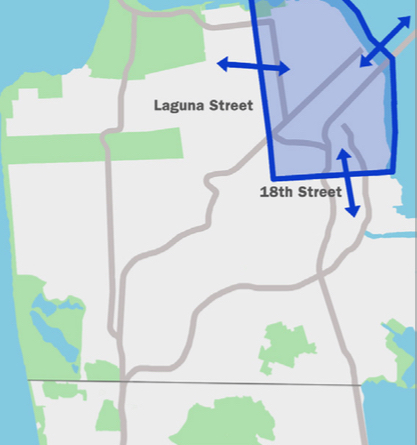
\includegraphics[width=0.4\textwidth]{chapter3/images/Fig3}
\caption{Northeast Cordon for San Francisco Congestion Pricing \citep{sfcta_san_2010}}
\label{fig:northeast_cordon}
\end{figure}

\subsubsection{TDM Analysis---Individualized Marketing}
\label{sec:application_tdm_analysis_procedures}
% Describe the procedures used for the TDM application
To better understand the differences between the standard MNL model and the asymmetric logit-type models developed in this chapter, we asked the following question. Given a fixed budget to be spent on the provision of month-long free transit passes (such as for an individualized marketing pilot program), how would using the various asymmetric choice models for target selection compare to using the MNL model in terms of the dollars spent per expected new transit-rider?

To answer this question, we needed:
\begin{itemize}
\item a way to calculate the costs of transit-pass provision for each targeted individual,
\item a way to select individuals for targeting given the choice model being used, and
\item a way to assess each targeted individual's change in the probability of transit usage, given free transit.
\end{itemize}
First, we calculated the total cost of transit-pass provision for each individual by multiplying each individual's cost of the ``walk-transit-walk'' mode by an assumed 22 working days per month. Although one might typically take the cost of a month-long transit pass from relevant transit agencies and use this as the cost of transit-pass provision for each individual, transit agencies in the San Francisco Bay Area such as the Bay Area Rapid Transit (BART) System and Caltrain use distance-based fares. As a result, such agencies do not offer monthly passes, and we based our cost calculations on the individualized transit costs instead of using a single cost for all individuals. The idea is that each individual would be provided with a transit-pass that has been preloaded with the amount of money that is deemed necessary for the individual to complete one walk-transit-walk commute tour per working day for a month.

Secondly, to select individuals for targeting, we assumed the role of an agency that was interested in (1) incentivizing individuals to use the ``walk-transit-walk'' mode and (2) maximizing the increase in the expected number of walk-transit-walk riders per dollars expended. Based on these goals, our target selection procedure was as follows. We first calculate the probability of using the walk-transit-walk mode with and without a transit pass. Note that the provision of a transit pass would completely eliminate the cost of the walk-transit-walk mode, but it would also reduce the cost of the walk-transit-drive and drive-transit-walk modes by however much the individual would pay in walk-transit-walk costs\footnote{Of course, we assumed a minimum cost of \$0.}. Next we divide the change in the walk-transit-walk probability by the total cost of transit provision for each person. Finally, we place the individuals in descending order according to their change in walk-transit-walk probabilities per dollar spent, and we select all individuals from the top of the list such that the total cost of the transit-pass provision for all selected individuals is less than our specified budget. We repeated our analysis for a range of different budgets (\$5,000 - \$60,000) to better understand how the models perform in different scenarios.

Lastly, to assess each targeted individual's change in the probability of transit usage, we had to choose a model to treat as ``truth.'' As shown in Section \ref{sec:application_results}, the uneven logit model had the best in-sample and out-of-sample log-likelihoods. Given the dominant performance of the uneven logit model, we treated it as the ``true'' model that would be used to calculate the probability of an individual taking transit with or without a free transit-pass. Each model's probability predictions were therefore used to select the individuals for targeting as described in the last paragraph, but the uneven logit model was used when assessing the ratio of the total cost of the individualized marketing program to the total increase in the expected number of walk-transit-walk riders.

As one reviewer pointed out, treating the uneven logit model as the ``truth'' may be viewed as problematic because the shape parameters of the uneven logit model have confidence intervals that include zero (the same value as the standard MNL model). However, the joint confidence region of the vector of uneven logit shape parameters definitely excludes the vector of all zeros (i.e. the standard MNL model). This can be seen by the statistically significant results of the likelihood ratio test of the uneven logit model versus the standard MNL. As a result, even though the shape parameters have some uncertainty associated with them, the joint uncertainty is not so large as to include the standard MNL model. Because of these observations, and because we still need to be able to compare each model's predictions with some notion of `truth,' we treat the uneven logit model as the `truth.' Moreover, we choose to not include bootstrapped confidence intervals in Figure \ref{fig:tdm_program_efficiencies}. The point of this plot is to illustrate that differences between the various logit-type models are to be observed at the disaggregate level. This point would remain, even if overlapping confidence intervals were displayed, as the means of these confidence intervals would remain as they are now.

\newpage
\renewcommand\bibname{{References}} %  will print ''References'' instead of ''BIBLIOGRAPHY''
\bibliographystyle{plainnat}
\bibliography{chapter3/current/ch3}


%\clearpage
%!TEX root = ../../../dissertation.tex

\chapter{Machine Learning Meets Microeconomics: \small{The Case of Decision Trees and Discrete Choice}}
\label{ch:4}

\begin{chapterabstract}
In the 1960's, the logistic regression model from statistics and the binary probit model from psychology were linked with random utility theory, thereby connecting such methods with economic theory. Since then, the fields of statistics, computer science, and machine learning have created numerous methods for modeling discrete choices. However, these newer methods have not been derived from or linked with economic theories of human decision making. We believe this lack of economic interpretation is one reason discrete choice modelers have been slow to adopt these newer methods.

This chapter begins bridging this gap by providing a microeconomic framework for decision trees: a popular machine learning method. Specifically, we show how decision trees represent a non-compensatory decision protocol known as disjunctions-of-conjunctions and how this protocol generalizes many of the non-compensatory rules used in the discrete choice literature so far. Additionally, we show how existing decision tree variants address many economic concerns that choice modelers might have. Beyond theoretical interpretations, we contribute to the existing literature of two-stage, semi-compensatory modeling and to the existing decision tree literature. In particular, we formulate the first bayesian model tree for classification, thereby allowing for uncertainty in the estimated non-compensatory rules as well as for context-dependent preference heterogeneity in one's second-stage choice model. Using an application of bicycle mode choice in the San Francisco Bay Area, we estimate our bayesian model tree, and we find that it is over 1,000 times more likely to be closer to the true data-generating process than a multinomial logit model (MNL). Qualitatively, our bayesian model tree automatically finds the effect of bicycle infrastructure investment to be moderated by travel distance, socio-demographics and topography, and our model identifies diminishing returns from bicycle lane investments. These qualitative differences lead the bayesian model trees to produce forecasts that directly align with the observed bicycle mode shares in regions with abundant bicycle infrastructure such as Davis, CA and the Netherlands. In comparison, the forecasts of the MNL model are overly optimistic.
\end{chapterabstract}


\section{Introduction}
\label{sec:introduction}
During the 1960s and 1970s, Daniel McFadden spearheaded the use of discrete choice techniques within economics, and in 2000, he was awarded a Nobel Prize for this work \citep{university_of_california_2000, manski_2001_daniel}. By his own account \citep{mcfadden_2001_economic}, McFadden's major contribution was \textit{not} the creation of the conditional logit\footnote{Note that the conditional logit model is also commonly referred to as the multinomial logit (MNL) model.} model---a model that is still one of the most widely used discrete choice methods today. Indeed, the concept of a random utility maximization model was created earlier by Jacob Marschak (\citeyear{marschak_1960_binary}), and statistical models that are nearly equivalent to McFadden's conditional logit model had already been introduced by David Cox (\citeyear{cox_1966_some}). According to McFadden,
\begin{quotation}
``The reason my formulation of the MNL model has received more attention than others that were developed independently during the same decade seems to be the direct connection that I provided to consumer theory [...].'' \citep[p. 354]{mcfadden_2001_economic}.
\end{quotation}
Put simply, the great contribution of McFadden's work is that he connected an existing statistical model of discrete outcomes with economic theory \citep{manski_2001_daniel}.

In the more than fifty years since McFadden's pioneering efforts, the fields of machine learning and statistics have produced a vast array of methods that, like discrete choice models, predict the probability that a given discrete outcome will be realized out of a finite set of discrete alternatives. We now have decision trees, kernel machines, neural networks, and much more \citep{bishop_2006_pattern, friedman_2008_elements, murphy_2012_machine}. In general, these new techniques often display superior predictive ability compared to traditional discrete choice models \citep{fernandez_2014_do, wainer_2016_comparison}. However, despite this smorgasbord of accurate methods, discrete choice modelers have mostly restricted themselves to econometric techniques that are descended from McFadden's conditional logit model \citep{manski_2001_daniel}.

We hypothesize that one reason machine learning models have not made greater inroads amongst discrete choice modelers is because these models have not been linked to economic theories of human decision-making. Moshe Ben-Akiva (\citeyear{ben_1973_structure}), one of the earliest discrete choice researchers, once wrote that ``a model can duplicate the data perfectly, but may serve no useful purpose for prediction\footnote{Note that the sort of prediction being referred to is prediction in the face of a policy change. This type of prediction is characteristic of causal inference whereby one predicts the effects of external manipulation of environmental conditions.} if it represents erroneous behavioral assumptions.'' Though written in the 1970's, we believe that this sentiment still pervades the field of discrete choice modeling and econometrics more broadly \citep{einav_2014_data, bajari_2015_demand, bajari_2015_machine}. As a result, econometricians do not make frequent use of alternative techniques from machine learning and statistics. Such methods may be useful for prediction under stationary conditions, but they are considered black-boxes that lack a theoretical basis for interpreting and understanding human behavior.

In contrast to newer techniques from statistics and machine learning, almost all discrete choice models in the literature are rooted in the theory of utility maximization \citep{train_2009_discrete}, and even competing discrete choice models are based on alternative behavioral theories such as regret minimization \citep{chorus_2012_random}. Overall, theory-based econometric techniques appear to have become dominant within econometrics because behavioral theories provide a way to understand and interpret one's model outputs beyond in-sample and out-of-sample predictive accuracy. Machine learning methods have yet to provide this additional framework and linkage with economic theory.

In this chapter, we aim to bridge this method-versus-theory gap by continuing to merge existing quantitative techniques with economic principles. Our contributions to the literature are as follows. First, we take a popular machine learning method---decision trees---and we connect it to economic theory. To do so, we provide a microeconomic framework for the interpretation of decision trees. In particular, we show that decision trees correspond to a non-compensatory, microeconomic decision protocol known as ``disjunctions-of-conjunctions'' \citep{hauser_2010_disjunctions}. Using this perspective, we explain how many of the varieties of decision trees address and can be motivated by microeconomic considerations such as analyst uncertainty or heterogeneity in one's non-compensatory behaviors. Additionally, our economic viewpoint suggests new additions to the existing body of decision tree techniques---additions that should lead to not only richer econometric models, but to more accurate statistical models overall.

Second, by combining decision trees with traditional discrete choice models, we advance the state of the art in the modeling of semi-compensatory decision making. We discuss how decision trees allow us to more flexibly represent non-compensatory behaviors than previously possible. Moreover, we show that our two-stage, semi-compensatory model jointly models how non-compensatory decision protocols influence both choice set formation and preference heterogeneity\footnote{We are aware that, in the discrete choice literature, the term preference heterogeneity has been used ambiguously. In some cases, preference heterogeneity refers to differences in the general preference for an alternative, irrespective of attributes of the alternative \citep{bhat_1998_accommodating}. In other cases, preference heterogeneity is taken to also include the coefficients that are multiplied by an alternative's attributes when using a linear-in-parameters choice model specification \citep{kamakura_1996_modeling}. In still other cases, preference heterogeneity is taken to also include choice set heterogeneity \citep{vij_2014_preference}. In this chapter, we use preference heterogeneity to include all of the coefficients in one's linear-in-parameters choice model specification. If one is using a non-linear or non-parametric choice model specification, we are also using preference heterogeneity to include differences in the systematic utility functions for different individuals.}.

Finally, our third contribution is an empirical demonstration of the aforementioned techniques to the choice of travel mode in the San Francisco Bay Area. We show that the semi-compensatory models fit the data better than traditional models based solely on utility-maximization, and we show that the semi-compensatory models lead to a number of policy implications that are not readily uncovered by traditional discrete choice models. Through this application, we illustrate the quantitative and qualitative benefits that can come from combining economic theory with machine learning and modern statistical methods.

Structurally, the rest of this chapter is organized as follows. In Section \ref{sec:decision-tree-explanation}, we provide an econometrically accessible introduction to decision trees. Here, we focus on decision trees as a statistical tool. Next, Section \ref{sec:decision-tree-economics} describes the microeconomic theories of non-compensatory decision making that are related to decision trees, and it shows how decision trees algorithmically represent these concepts. Here, we focus on the ways that decision trees are motivated by particular decision making principles. In Section \ref{sec:literature-review}, we review how the aforementioned microeconomic concepts have been operationalized in the discrete choice literature so far, and we make note of how decision trees address the theoretical and practical difficulties with these previous implementations. Section \ref{sec:decision-tree-variants} then details the various types of decision trees, including combined decision-tree/discrete-choice models. Specifically, we orient our discussion around the ways these decision tree variants address economic considerations that might prevent choice modelers from using decision trees in their work. In Section \ref{sec:empirical-application}, we formulate a new decision-tree/discrete-choice model, and we apply the model to the choice of travel mode in the San Francisco Bay Area. We describe the data used for this application, and we discuss the greater fit and unique insights provided by our semi-compensatory model in comparison to models based purely on utility-maximization. Finally, Section \ref{sec:conclusion} concludes.

\section{Decision trees explained}
\label{sec:decision-tree-explanation}
In this section, we provide a brief description of decision trees, targeting econometricians as our main audience. We will first provide an explanation of what a decision tree is, and we will use a highly simplified example to demonstrate how they can be used. After this, we will give a brief description of some of the (many) ways that decision trees are estimated from data. Here, again, we will focus on comparing and contrasting these estimation methods with techniques that econometricians are familiar with.

\subsection{What are decision trees and how do we use them?}
\label{sec:what-are-dtrees}
In simple terms, decision trees are a set of ``if-then'' statements that are used to predict a given quantity\footnote{We realize that our definition of decision trees is broad. Our definition includes models such as regression trees, classification trees, decision lists, and decision tables \citep{rivest_1987_learning, loh_2011_classification}. For this chapter's purposes, these models are similar enough to merit a joint description.} \citep{loh_2011_classification}. Etymologically, decision trees get their name because they are often represented graphically as a tree: an acyclic set of nodes connected by directed edges, with each node connected to at most one preceding node, beginning with a single ``root'' node that has no edges pointing into it, and terminating with a set of ``output'' nodes \citep{meila_2000_learning, rokach_2005_top}. Each path from the root node to an output node represents one of the ``if-then'' statements that make up the tree. These if-then statements must partition the space of explanatory variables into a set of mutually exclusive regions (corresponding to the output nodes) that span the entire space of explanatory variables \citep{lemon_2003_classification}. Then, when making predictions about a decision maker, the ``if'' condition is used to determine the region/output-node the decision maker is in, and the corresponding ``then'' statement is used to provide the desired prediction. In a discrete choice context, such predicted quantities might be (1) the probability that a particular alternative is considered or (2) the probability with which an alternative is chosen.

\begin{figure}
\centering
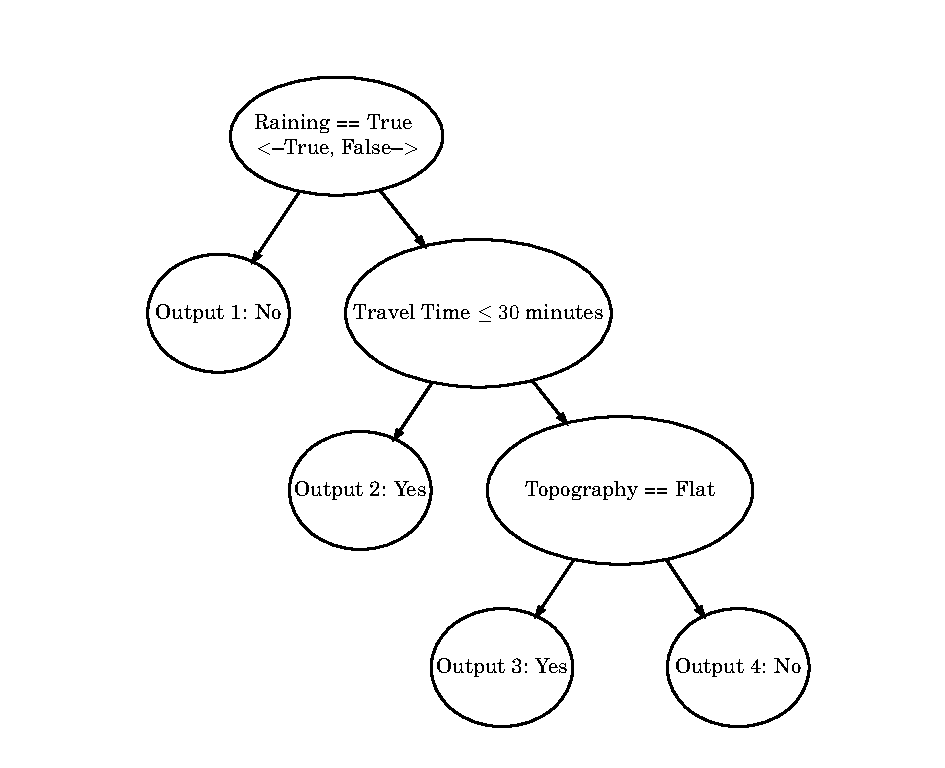
\includegraphics[width=0.5\textwidth]{chapter4/images/example_tree_bicycle}
\caption{Example decision tree for bicycle consideration}
\label{fig:tree-for-bicycle-consideration}
\end{figure}

To continue our explanation of what decision trees are and how they can be used, we will now provide a concrete, but highly stylized example of choice set generation, conditional on a given decision tree. In the discussion that follows, we realize that modelers may have many valid reservations about the realism of our example. It suffices to say that concerns about the deterministic nature the choice sets generated by our tree (shown in Figure \ref{fig:tree-for-bicycle-consideration}), concerns about the explicit discontinuities in the tree, and concerns about how such a tree could be estimated can all be addressed. Our example only features these qualities for simplicity of discussion. We note that in some contexts, deterministic choice sets are not uncommon: for example, when individuals are making residential location choices, some housing options may be deterministically excluded because the rents violate the individuals' income constraints \citep{kaplan_2012_development, zolfaghari_2013_simplified, bhat2015comprehensive}. Moreover, decision trees that probabilistically predict an individual's choice set can be estimated. These considerations will be discussed in Section \ref{sec:decision-tree-variants}. Concerns about the explicit discontinuities in our tree can be relaxed by considering individual heterogeneity in the split points of a tree or in the very structure of the tree being used. Like the issue of estimating trees that probabilistically predict an individual's choice set, concerns about individual heterogeneity are discussed in Section \ref{sec:decision-tree-variants}. Lastly, the estimation of decision trees will be discussed in Subsection \ref{sec:how-to-estimate-dtrees}.
 
Now, disclaimers aside, imagine that we are modeling the choice set formation behavior of travellers who are choosing the mode by which they will travel. Further, assume that our population of individuals has only two commuting alternatives: bicycle and public transit, and assume that public transit is always considered. Finally, Figure \ref{fig:tree-for-bicycle-consideration} shows the decision tree that represents the assumed choice set formation process in our hypothetical population. Here, \textit{Raining} is either \textit{True} or \textit{False}, \textit{Travel Time} is measured in minutes, \textit{Topography} is either \textit{Flat} or \textit{Hilly}, and the dependent variable (bicycle consideration) is either \textit{Yes} or \textit{No}. From the tree in Figure \ref{fig:tree-for-bicycle-consideration}, a number of useful observations can be made. First, there are four output nodes, two of which result in bicycle being considered and two that result in bicycle not being considered. Secondly, we see that bicycle consideration is a function of weather (raining or not), travel time, and topography. Now, to use the tree to make predictions for a given individual, one must traverse the tree from top to bottom, ending at one of the tree's output nodes. The rules for traversing the given\footnote{We note in passing that the traversal rules may change from tree to tree, based on author preference, but they should always be explicitly stated.} decision tree are that if the condition in a decision node (i.e. a non-output node) is True, then one goes to the left and if the condition is False, one goes to the right.

So, what can one use the tree in Figure \ref{fig:tree-for-bicycle-consideration} for? First, the tree and its predictions can be directly used to inform policies. For instance, a municipality trying to increase bicycle usage must first ensure that bicycle is considered as a mode of travel. Based on this example's tree, the municipality might subsidize the relocation costs for individuals that wish to move to a location that is 30 minutes away or closer to their workplace. Such subsidies would help push bicycle into the choice sets of individuals, thereby increasing the expected number of bicycle commuters. Secondly, the tree in Figure \ref{fig:tree-for-bicycle-consideration} might be used as part of a larger model building effort. For instance, one might use the tree in Figure \ref{fig:tree-for-bicycle-consideration} to inform a two-stage model of travel mode choice. At the first stage, an individual's choice set is modeled. By assuming that individuals must travel to work and that public transit is always considered, our example is left with two possible choice sets: \{Public Transit\} and \{Public Transit, Bicycle\}. The choice sets in this example are based on whether bicycle is considered or not, and the probabilities of these choice sets (i.e. the first stage in Manski's two-stage models) can be written as follows:
\begin{equation}
\begin{aligned}
P \left( C = \left\lbrace \textrm{Public Transit, Bicycle} \right\rbrace \mid x, \textrm{tree} \right) &= P \left( \textrm{Bicycle considered} \mid x, \textrm{tree} \right)\\
&= \sum _r P \left[ \textrm{Bicycle considered} \mid T \left( x \right) = r \right] P \left[ T \left( x \right) = r \right]\\
\textrm{where } C &= \textrm{An individual's choice set.}\\
r &\in \left\lbrace 1, 2, 3, 4 \right\rbrace\\
r &= \textrm{A specific region demarcated by the decision tree.}\\
T \left( x \right) &= \textrm{The region an individual belongs in based on $x$ and the tree.}\\
x &= \textrm{Explanatory variables for an individual.}
\end{aligned}
\end{equation}

For most decision trees, $T \left( x \right)$ is a deterministic function\footnote{The primary exception to this is a ``probabilistic'' decision tree, also known as a ``soft'' or ``fuzzy'' decision tree, where $T \left (x \right)$ is a probabilistic function. These decision tree variants will be discussed in Section \ref{sec:decision-tree-variants}. The other exception is where the case of measurement error where the value $x$ is unknown and modeled with a probability distribution of its own.} such that, given explanatory variables $x$, an observation is deterministically assigned to a given region/output-node $r$. For our example, regions 2-4 are graphically depicted in Figure \ref{fig:regions-of-tree}. Because our $T \left( x \right)$ is deterministic, $P \left[ T \left( x \right) = r \right]$ is either 1 or 0, and the same is true of the probability of bicycle consideration, conditional on being in a given region. In all cases, we can expand $P \left[ T \left( x \right) = r \right]$ to more explicitly show how each explanatory variable contributes to the likelihood of an observation being in a given region.

\begin{figure}
\centering
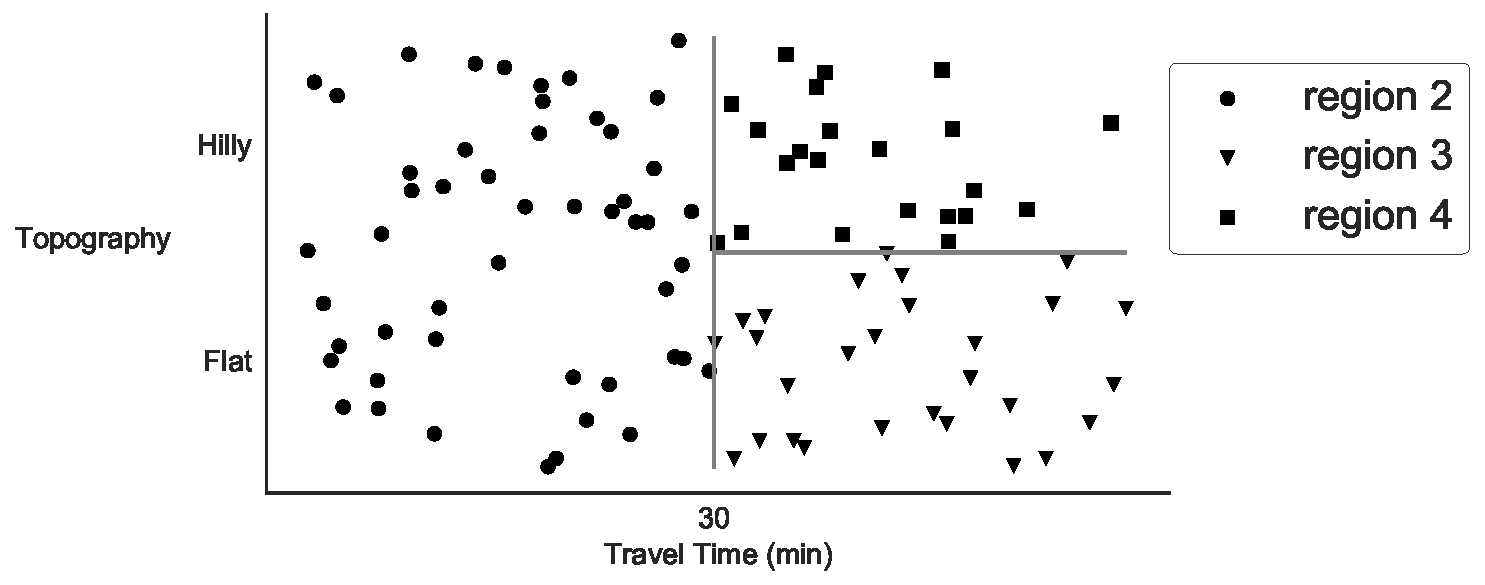
\includegraphics[width=0.75\textwidth]{chapter4/images/region_plot}
\caption{Regions 2-4 of example decision tree for bicycle consideration}
\label{fig:regions-of-tree}
\end{figure}

Specifically, we note that each ``if'' statement in the decision tree can be written as the union of elementary conditions, typically\footnote{Exceptions to this statement come from decision trees that are not ``axis-aligned,'' such as oblique decision trees that use inequalities with linear combinations of variables for their ``if'' conditions \citep{murthy_1994_system, ittner_1996_non}.} with one such elementary condition per explanatory variable. For instance, let $x_1$ denote whether it is raining, let $x_2$ denote the bicycle travel time between an individual's home and work, and let $x_3$ denote the topography between an individual's home and work. Additionally, let $S_{rk}$ denote the set that variable $x_k$ must be in for an individual to belong to region $r$. Using these variables, we can write the region corresponding to the first output node as $S_{11} = \left\lbrace \textrm{True} \right\rbrace$, $S_{12} = \left[ 0, \infty \right)$, and $S_{13} = \left\lbrace \textrm{Flat, Hilly} \right\rbrace$. These sets reflect the fact that output node 1 is the region of the variable space where \textit{Raining} is True and where any values of \textit{Travel Time} or \textit{Topography} are valid. With this notation, we can express the probability of bicycle consideration as follows:

\begin{equation}
\label{eq:consideration-likelihood}
\begin{aligned}
P \left( \textrm{Bicycle considered} \mid x, \textrm{tree} \right) &= \sum _r P \left[ \textrm{Bicycle considered} \mid T \left( x \right) = r \right] P \left[ T \left( x \right) = r \right]\\
&= \sum _r P \left[ \textrm{Bicycle considered} \mid T \left( x \right) = r \right] P \left[ \bigcap _k x_k \in S_{rk} \right]\\
&= \sum _r \left\lbrace P \left[ \textrm{Bicycle considered} \mid T \left( x \right) = r \right] \prod _k P \left[ x_k \in S_{rk} \right] \right\rbrace
\end{aligned}
\end{equation}

The equation above shows how, conditional on a given decision tree, one can form the sorts of probability statements that are common in the first stage of two-stage choice models with non-compensatory rules for choice set formation \citep{gilbride_2004_choice, cantillo2006discrete}. Moreover, if one's decision tree was being used to directly predict the probability of a given alternative, one's likelihood function would be formed analogously. Besides being transparent about how the structure of the tree translates to one's likelihood equations, Equation \ref{eq:consideration-likelihood} highlights the link to the non-compensatory decision protocol known as disjunctions-of-conjunctions \citep{hauser_2010_disjunctions}. Though we will delay a detailed discussion of this protocol to Section \ref{sec:decision-tree-economics}, we point out here that logical disjunctions are algebraically represented as summations and logical conjunctions are algebraically represented as products \citep{gilbride_2004_choice}. Equation \ref{eq:consideration-likelihood} shows that when modeling bicycle consideration with a decision tree, our probabilities of interest are explicitly given as a summations of products (i.e as disjunctions-of-conjunctions). Importantly, such a decision protocol generalizes the typical conjunctive or disjunctive rules that are used in choice models that represent non-compensatory processes. See Section \ref{sec:decision-tree-economics} for further discussion and explanation of this point.

\subsection{How do we estimate decision trees?}
\label{sec:how-to-estimate-dtrees}
In the previous subsection, we explained what decision trees are and (conditional on a specific decision tree) what one can do with them. In this subsection, we turn to the question of how such decision trees are estimated from data and how such estimation techniques differ from those commonly employed in the discrete choice literature.

To begin, discrete choice modelers are most likely to be familiar with estimation techniques such as maximum likelihood, method of moments, and bayesian Markov Chain Monte Carlo (MCMC) methods \citep{train_2009_discrete}. Of these techniques, only bayesian MCMC methods have been applied to the estimation of decision trees \citep{chipman_1998_bayesian, denison_1998_bayesian, letham_2015_interpretable, pratola_2016_efficient}. We believe that the main reason for this discrepancy in estimation methods is that decision trees are not continuous functions. Instead, they are explicitly discontinuous functions of the explanatory variables (e.g. at a particular node, should we split on \textit{Travel Time} or \textit{Travel Cost}?). Maximum likelihood, if it is to be performed at all can no longer rely on gradients and hessians, so enumeration and comparison of all decision trees is necessary. However, enumeration of all possible decision trees is NP-hard \citep{ruggieri_2017_enumerating}. Since it is computationally prohibitive to enumerate all possible decision trees and assess their log-likelihoods, maximum likelihood estimation of decision trees is typically viewed as infeasible. Similarly, since the method of moments and its generalizations require continuous moment functions \citep{hansen_1982_large}, these estimation techniques cannot be used to estimate decision trees.

As highlighted in the last paragraph, estimation of decision trees is severely hindered by the discontinuous nature of the trees and the fact that explicit enumeration of all possible trees is computationally prohibitive. Due to these challenges, most estimation techniques (both bayesian and frequentist) use approximations and heuristics. By far, the most common frequentist heuristic is to use a greedy algorithm to estimate the tree \citep{rokach_2005_top}. Here, one recursively performs a search over all variables and values of those variables to pick the variable and value combination that best meets some ``splitting criteria.'' After finding the best variable and value pair, the dataset is split according to the chosen pair. The process is then repeated for each subset of the data: those meeting the chosen condition and those not meeting the condition. The greedy estimation of the decision tree will terminate once some stopping criteria is met (e.g. no output node should contain less than 5 observations). After the initial estimation of the decision tree, some estimation methods ``prune'' the initial tree by removing nodes according to a ``pruning criterion'' \citep{mingers_1989_empirical, esposito_1997_comparative}. Differing methods and criteria for splitting, stopping, and pruning all lead to different types of decision trees \citep{loh_2014_fifty, rokach_2014_data}. Moreover, besides the greedy approach just described, there exist a number of other frequentist tree estimation techniques such as using genetic algorithms \citep{barros_2012_survey} or branch-and-bound algorithms \citep{angelino_2017_learning}. Though we cannot perform an exhaustive review of the various decision tree estimation techniques, good surveys of this material can be found in \citet{murthy_1998_automatic, rokach_2005_top, barros_2012_survey}, and \citet{lomax_2013_survey}.

For the bayesian estimation of decision trees, a prior is placed over the space of possible decision trees, the likelihood is formed using equations similar to Equation \ref{eq:consideration-likelihood}, and then an MCMC algorithm is used to sample from the posterior distribution of possible decision trees \citep{chipman_1998_bayesian, denison_1998_bayesian, letham_2015_interpretable, pratola_2016_efficient}. At first glance, this seems exactly the same as what is always done in a bayesian estimation. However, since the set of all possible decision trees is huge and discrete, the MCMC algorithms do not typically ``explore'' the entire posterior distribution of trees \citep{chipman_1998_bayesian}. The approximation is that the MCMC methods typically only explore part of the posterior since these algorithms are limited by however much time an analyst has to let the algorithm run. If the MCMC algorithm is run for long enough, the hope is that ``high accuracy'' sections of the posterior are explored, such that one samples from the trees that are most predictive of the choices in one's dataset. Note, unlike the frequentist estimation methods where trees are defined based on how they are estimated, differing priors or differing MCMC methods lead to differences in how the space of decision trees is explored, but it is uncommon to speak of ``different'' bayesian decision trees. Such differentiation is likely unnecessary because, given an impractically long time, all bayesian MCMC techniques will explore the entire posterior of trees.

Finally, we pause to make a few passing remarks about the properties of the various estimators for decision trees. In standard discrete choice modeling, much importance is placed on having consistent and efficient estimators. The greedy estimation techniques described above for decision trees have long been proven to be consistent, non-parametric estimators of underlying data-generating processes \citep{gordon_1980_consistent, gordon_1984_almost, toth_2011_building}. Bayesian techniques have also demonstrated their consistency in simulation \citep{letham_2015_interpretable}, though formal proofs are still missing. In terms of efficiency, however, it is not clear that this notion is meaningful for decision tree models. In particular, the notion of an ``efficient'' estimator being one that achieves the Cramer-Rao lower bound is no longer meaningful since the parameter space (the number of splits in the tree, variables and values being split on, and the tree structure) is discrete and increases with the size of one's data set (i.e. it is not fixed). If one views efficiency as being inversely related to the variance of one's estimator, then it is known that estimation techniques that generate a large number of candidate trees and then select the best one tend to be less variable than the greedy methods described above \citep{tibshirani_1999_model}. Nevertheless, whether or not other variations on the notion of efficiency can be shown to apply to decision trees is beyond the scope of this chapter and will not be investigated.


\section{Decision trees: The link with microeconomics}
\label{sec:decision-tree-economics}
In Section \ref{sec:decision-tree-explanation}, we described what decision trees are, how a given decision tree can be used, and how decision trees might be estimated. Additionally, in both Sections \ref{sec:introduction} and \ref{sec:decision-tree-explanation}, we noted that decision trees correspond to a non-compensatory decision protocol known as disjunctions-of-conjunctions \citep{hauser_2010_disjunctions}. In this section we will review this microeconomic interpretation of decision trees in detail. Initially, we will briefly describe standard discrete choice models and their use of compensatory decision protocols. Then we will motivate the need for non-compensatory decision protocols, and in Subsection \ref{sec:noncompensatory-description}, we will proceed to describe a number of such behavioral strategies. We will begin with simple non-compensatory protocols and proceed to describe further generalizations of such strategies until we arrive at disjunctions-of-conjunctions: a focal point of this chapter. Finally, in Subsection \ref{sec:dtrees-and-disjunctions-of-conjunctions}, we will mathematically show how decision trees represent disjunctions-of-conjunctions.

To start, we note that compensatory decision protocols are decision making strategies where, for a given alternative, ``high levels of satisfaction with one attribute compensate for low levels of satisfaction with [other]'' attributes \citep{foerster1979mode}. As readers are likely aware, almost all discrete choice models used in practice and research are based on compensatory decision processes, with utility-maximization being the most common example\footnote{We are aware of the increasing number of discrete choice models that are being estimated under the assumption of regret-minimizing behavior. However, such models are still compensatory in nature, and therefore retain many of the properties we describe in the context of utility-maximization.} \citep{swait_2001_non, truong_2015_modeling}. However, counter to prevailing practices, behavioral economists and psychologists have presented much evidence that individuals frequently depart from standard notions of utility maximization and rationality \citep{foerster1979mode, bronner_1982_decision, tversky_1986_rational, conlisk_1996_why}. Spurred by these observations, a steady but small stream of research has both called for and proposed new models of human decision making that explicitly incorporates the possibility of non-utility maximizing choice behavior \citep{simon_1955_behavioral, tversky_1972_elimination, gigerenzer_1996_reasoning, leong_2012_embedding}. Such alternative methods of decision making are typically referred to as non-compensatory decision rules or non-compensatory decision protocols. They are called non-compensatory because they do not always allow positive attributes of a given alternative to compensate for negative attributes of that same alternative. Additionally, since non-compensatory decision rules do not typically require the evaluation of all attributes of all alternatives, they better capture the limited cognitive resources of decision makers \citep{simon_1955_behavioral, young_1984_non, swait_2001_non} and are therefore thought to be more behaviorally realistic.

\subsection{Non-compensatory decision rules}
\label{sec:noncompensatory-description}
Thus far, some of the non-compensatory decision processes that have been detailed in the discrete choice literature include: dominance \citep{cascetta2009dominance}, lexicography \citep{kohli2007representation}, elimination-by-aspects \citep{tversky_1972_elimination}, satisficing \citep{stuttgen2012satisficing}, conjunctive rules, disjunctive rules, subset-conjunctive rules, and disjunctions-of-conjunctions. Of these, conjunctive and disjunctive rules are quite prevalent in the literature, and all of the last four non-compensatory rules are related to decision trees. We therefore describe the last four non-compensatory decision protocols below, and in Section \ref{sec:literature-review}, we review how these four protocols have been previously incorporated into discrete choice models.

\begin{description}
\item [Conjunctive Rules \citep{coombs_1951_mathematical, dawes_1964_social}] \hfill \newline
Using a conjunctive decision rule, an individual only considers alternatives that meet all of a given number of requirements. For instance, an individual making a residential location choice may only consider housing options that meet his or her requirements on the maximum amount of rent \textbf{and} the distance from the individual's workplace location. The ``and'' statement is what distinguishes this decision rule as conjunctive. As noted in Subsection \ref{sec:what-are-dtrees}, conjunctive statements are algebraically represented using products.

\item [Disjunctive Rules \citep{coombs_1951_mathematical, dawes_1964_social}] \hfill \newline
Using a disjunctive decision rule, individuals only consider alternatives that meet at least one of a given set of requirements. For instance, continuing with the residential choice example, an individual may only consider housing options that are within a given distance from their workplace location \textbf{or} that are within a given distance from major public parks. The ``or'' statement is what distinguishes this decision rule as disjunctive. As noted in Subsection \ref{sec:what-are-dtrees}, disjunctive statements are algebraically represented using sums.

\item [Subset-Conjunctive Rules \citep{jedidi_2005_probabilistic}] \hfill \newline
Subset-conjunctive rules are a generalization of both conjunctive rules and disjunctive rules. Using a subset-conjunctive decision rule, an individual only considers alternatives that meet a certain number of requirements. Using another residential location choice example, consider an individual who would like to live within one mile of a major public park, who would like to live within two miles of his or her workplace, who would like to pay less than \$1,000 per month in rent (but is flexible), and who would like to live within one mile of a subway station. Under a subset-conjunctive rule, this individual would consider any housing units that meet some number of these four requirements. For instance, this individual might consider any housing units that meet at least three of these four requirements. Note that if this individual only considered housing units that met all four requirements, then this would be equivalent to a conjunctive decision rule with four requirements. Likewise, if this individual only required housing units to meet one of the four requirements, then this would be equivalent to a disjunctive decision rule. Algebraically, subset-conjunctive rules are therefore sums of products, with the restriction that each product term have a given number elements (one for each requirement that should be met).


\item [Disjunctions-of-Conjunctions \citep{hauser_2010_disjunctions}] \hfill \newline
Disjunctions-of-conjunctions generalize the conjunctive, disjunctive, and subset-conjunctive decision rules. Under a disjunctions-of-conjunctions decision protocol, an individual will consider any alternative that meets at least one of a given set of conjunctive conditions. Each condition may differ in the number of requirements that compose the conjunction. Algebraically, then, disjunctions-of-conjunctions are expressed as sums of products with no constraints on the number of elements in each product.

Consider once more the residential choice example. If, for instance, our decision maker was more concerned about rent than the other requirements, he or she might consider any housing unit that required less than \$1,000 per month in rent and that met one of the remaining three requirements. Additionally, he or she might consider any housing unit that was simultaneously within one mile of a major park, within one mile of a subway station, and within two miles of his or her workplace. In this case, only one of the following four conjunctive conditions needs to be met in order for a housing unit to be considered:
\begin{itemize}
\item rent less than \$1,000 per month and housing unit within one mile of a major public park

\item rent less than \$1,000 per month and housing unit within two miles of the individual's workplace

\item rent less than \$1,000 per month and housing unit within one mile of a subway station

\item housing unit within one mile of a major public park and within one mile of a subway station and within two miles of the individual's workplace.
\end{itemize}

As can be seen from the example above, if the individual had only one condition for consideration, we would have a conjunctive rule. If the individual had only one requirement in each of the four conditions above, then we would have a disjunctive rule. Similarly, if we expanded the first three conditions above so that they each included a third requirement, we would once again have the subset-conjunctive rule whereby any housing unit with three of the four requirements would be considered.
\end{description}

Before moving on to Subsection \ref{sec:dtrees-and-disjunctions-of-conjunctions}, we pause to briefly summarize why we believe the link between disjunctions-of-conjunctions and decision trees is important. First, as noted above, conjunctive rules and disjunctive rules are seen as important information processing strategies, and they have been applied in many choice modeling efforts \citep{foerster1979mode, swait_2001_non, gilbride_2004_choice, elrod_2004_new, martinez_2009_constrained, hauser_2010_disjunctions, hess2012allowing, kaplan_2012_development, zolfaghari_2013_simplified, truong_2015_modeling}. Being a generalization of these two rules, disjunctions-of-conjunctions may also be an important decision making strategy, but it has seldom been tested in choice modeling contexts. We think a major reason for this lack of choice modeling application is because there have not been easy or straightforward ways to estimate such rules. Linking disjunctions-of-conjunctions to decision trees gives researchers a way to estimate disjunctions-of-conjunctions by drawing upon well established methods of estimating decision trees. Additionally, once disjunctions-of-conjunctions can be estimated by themselves, it is then possible to estimate such strategies in combination with the compensatory procedures used in standard discrete choice models. We pursue this strategy later, in Section \ref{sec:decision-tree-variants} and Section \ref{sec:empirical-application}.

\subsection{Linking decision trees with disjunctions-of-conjunctions}
\label{sec:dtrees-and-disjunctions-of-conjunctions}
As described in the previous subsection, disjunctions-of-conjunctions are highly flexible non-compensatory decision protocols. Here, we highlight how decision trees mathematically represent the relationships implied by disjunctions-of-conjunctions.

First, we define the necessary notation. Let $b$ represent a primitive boolean statement, i.e. a specific requirement. Such a statement is an equality or inequality that is not composed of any other equalities or inequalities. For instance, $x == 2$ and $x \leq 5$ are primitive boolean statements but ($\left( x_1 == 2 \right) * \left( x_2 \leq 5 \right)$) is not a primitive boolean statement because it is composed of two boolean statements. Additionally, if $b$ is True, then we say that $b = 1$, and if $b$ is False, then we say that $b = 0$.

With this notation, conjunctive rules can be expressed as:
\begin{equation}
\begin{aligned}
\textrm{if } \left( \prod _{i = 1} ^{B} b_i \right) &== 1 \Rightarrow y\\
\textrm{where } B &= \textrm{the total number of requirements in the rule.}\\
\textrm{``$\Rightarrow$''} &= \textrm{``then'' or ``implies''.}\\
y &= \textrm{some outcome.}
\end{aligned}
\end{equation}
In words, this is read as ``if all requirements, $b_i$, are met, then $y$''. This follows because each $b_i$ must be True (i.e. must be met) in order for that $b_i$ to equal 1, and we need all $b_i$ to equal 1 in order for $\prod _{i = 1} b_i$ to evaluate to 1.

Similarly, a disjunctive rule can be expressed as:
\begin{equation}
\textrm{if } \left( \sum _{i = 1} ^{B} b_i \right) \geq 1 \Rightarrow y
\end{equation}
In words, this is read as ``if at least one (i.e. if any) of the requirements $b_i$ are met, then $y$''. This follows because any requirement $b_i$ that is not met will cause that $b_i$ to evaluate to 0. If at least one requirement is met, then the corresponding $b_i$'s will evaluate to 1, and then $\sum _{i = 1} b_i$ will be greater than or equal to 1.

With these building blocks, we turn immediately to the case of disjunctions-of-conjunctions\footnote{Subset-conjunctive rules will be expressed as a special case of the formula for disjunctions-of-conjunctions.}. In words, the use of disjunctions-of-conjunctions requires statements such as ``if at least one of some set of conjunctive conditions is met, then $y$.'' To mathematically express such a statement, we will introduce additional symbols. The first symbol, $p$, will represent conjunctive conditions, i.e. products of primitive boolean statements. As noted in Subsection \ref{sec:noncompensatory-description}, in disjunctions-of-conjunctions, the various conjunctive conditions need not have the same number of requirements. To account for this, we will index the various conjunctive conditions by $i$, and we will use $\mid p_i \mid$ to denote the number of requirements that make up $p_i$. Finally, we will use the symbol, $b_j ^i$, to indicate the $j$'th primitive boolean statement (i.e. the $j$'th requirement) in conjunctive statement $p_i$. With this additional notation, our disjunctions-of-conjunctions statement can now be expressed as:
\begin{equation}
\begin{aligned}
\textrm{if } \left( \sum _{i = 1} ^{D} p_i \right) &\geq 1 \Rightarrow y\\
\textrm{if } \left( \sum _{i = 1} ^{D} \prod _{j = 1} ^{\mid p_i \mid} b_j ^i \right) &\geq 1 \Rightarrow y\\
\textrm{where } D &= \textrm{the total number of conjunctive conditions.}
\end{aligned}
\end{equation}
From the first line, we mathematically see the disjunction (i.e. the summation) of conjunctive conditions. The second line shows the conjunction (i.e. the product) of requirements. Now, for subset-conjunctive rules, we merely impost the constraint that $\mid p_i \mid$ be equal to some constant value for all $p_i$. This is equivalent to saying that each conjunctive condition must be comprised of the same number of requirements.

To go from the abstract equations above to a decision tree, we must consider what a conjunctive condition represents. In general, a conjunctive condition defines a region in a space. Using Figure \ref{fig:tree-for-bicycle-consideration} as an example once more, consider the space formed by the variables $x_1 = \textrm{Rain}$ and $x_2 = \textrm{Travel Time}$. The conjunctive condition that leads to output node 2 is $x_1 == \textrm{False}$ AND $x_2 \leq 30$. This condition will define a rectangular region in the graph of $\left( x_1, x_2 \right)$ comprised of the area where $x_1$ is False, and the area where $x_2$ is less than 30. For more examples of regions formed by conjunctive conditions, see Figure \ref{fig:regions-of-tree} above. Now, when we have multiple conjunctive conditions, we have multiple regions in space. These regions will either be mutually exclusive, or they will overlap. It is crucial to note that any region defined by a set of overlapping conjunctive criteria can be expressed as a region defined by a set of mutually exclusive criteria. For instance, let $\left\lbrace p \right\rbrace = \left\lbrace p_1, p_2 \right\rbrace$ be a region defined by a set of overlapping conjunctive conditions, $p_1$ and $p_2$. This region can be re-expressed as a set of mutually exclusive conjunctive conditions, $\left\lbrace \tilde{p} \right\rbrace = \left\lbrace \tilde{p}_1, \tilde{p}_2 \right\rbrace$. One such re-expression is $\tilde{p}_1 = p_1$ and $\tilde{p}_2 = p_2 * p_{1}'$, where $\tilde{p}_2$ is read as ``$\tilde{p}_2$ equals $p_2$ AND NOT $p_1$.'' Observations meeting the condition $\tilde{p}_2$ will therefore satisfy all the requirements of $p_2$, but they will not satisfy all the requirements of $p_1$.

With the possibility of re-expression in mind, recall that using disjunctions-of-conjunctions means making statements of the form ``if at least one of some set of conjunctive conditions, $\left\lbrace p \right\rbrace$, is met, then $y$''. As just noted, this statement can be reformulated as, ``if at least one of some set of conjunctive conditions, $\left\lbrace \tilde{p} \right\rbrace$, is met, then $y$''. Given the mutually exclusive conjunctive conditions of $\left\lbrace \tilde{p} \right\rbrace$, our reformulation can be expressed as a decision tree where each conjunctive condition in $\tilde{p}$ becomes an ``if'' statement in the tree with a corresponding ``then $y$'' statement. Note we will also need a final condition such as ``if $\bigcap _{i=1} ^{D} \tilde{p}_{i}'$ then $y'$,'' where $y' \neq y$. Here, the final condition ensures that the decision tree is comprised of a set of conditions that are both mutually exclusive and exhaustive. The condition $\bigcap _{i=1} ^{D} \tilde{p}_{i}'$ is read as ``NOT $\tilde{p}_1$ and NOT $\tilde{p}_2$ and ... and NOT $\tilde{p}_D$.'' Finally, we use $y'$ as the outcome for the remaining conditions that are added to ensure exhaustiveness, e.g. $\bigcap _{i=1} ^{D} \tilde{p}_{i}'$, simply because we assume that if there was any other condition that would result in $y$, then that condition would have been part of the original set of conditions, $\left\lbrace p \right\rbrace$.

\section{A review of how non-compensatory protocols have been incorporated in discrete choice}
\label{sec:literature-review}
In Section \ref{sec:decision-tree-economics}, we described conjunctive rules, disjunctive rules, subset-conjunctive rules, and disjunctions-of-conjunctions. However, researchers have gone beyond mere descriptions. These decision protocols have been incorporated into choice models and used to quantitatively study the concordance of non-compensatory processes with observed choices. In this section, we will review the ways that conjunctive rules, disjunctive rules, and their generalizations have been previously incorporated into discrete choice models. Afterwards, we will highlight drawbacks of the previous work that this chapter seeks to address. Having said this, we state upfront that our review mainly focuses on the way that non-compensatory protocols have been used to model choice set generation as opposed to modeling the actual choice being made. The reason for our focus is that conjunctive rules, disjunctive rules, and their generalizations are (in general) not sufficient to uniquely choose a particular alternative. Multiple alternatives may meet an individual's non-compensatory rules, but (in our context) a decision strategy must still be employed to generate a single discrete choice. As a result, conjunctive rules, disjunctive rules, and their generalizations have almost exclusively been used in the discrete choice literature to winnow a decision maker's choice set before another strategy is used (if necessary) to make the final choice. In Subsection \ref{sec:choice-set-generation-review}, we review this approach of choice set generation followed by compensatory choice amongst the considered alternatives, and we revisit this notion in Section \ref{sec:dtree-variants-preferences} when we describe the decision tree variant known as ``model trees.'' In Subsection \ref{sec:direct-modeling-review}, we will briefly review the few ways that observed choices have been directly\footnote{I.e., without estimating any rules or parameters that implicitly or explicitly determine one's choice set.} modeled with conjunctive rules, disjunctive rules, and their generalizations. 

\subsection{Choice-set generation via non-compensatory protocols}
\label{sec:choice-set-generation-review}
Across the literature, two main approaches have been used to incorporate conjunctive, disjunctive, and related protocols into discrete choice models. These two approaches differ primarily based on whether they explicitly model an individual's decision making using two-stages as prescribed by \citet{manski_1977_structure} or whether they use a single-stage model that implicitly performs choice-set generation. We will begin by first describing the single-stage models, also known as the ``reduced-form'' approach \citep{swait_2001_non}.

Pioneered by Swait (\citeyear{swait_2001_non}), single-stage models implement conjunctive and/or disjunctive rules by altering the systematic utility of an alternative. When representing strict non-compensatory behaviors, these models combine attribute values and attribute thresholds to set the systematic utility of an alternative to -/+ infinity, effectively removing an alternative from one's choice set or removing all other alternatives from one's choice set. Through the years, multiple single-stage models have been proposed, each with their own set of unique additions. \citet{swait_2001_non} allowed for non-strict non-compensatory behavior where violation of an attribute threshold was allowed but resulted in penalties to one's systematic utility. \citet{elrod_2004_new} estimated the attribute thresholds from choice data only, whereas \citet{swait_2001_non} required individuals to report their attribute thresholds. Moreover, \citet{elrod_2004_new} did not allow violation of one's attribute threshold and even penalized or rewarded the systematic utility when the value of an attribute approached that attribute's threshold, based on whether a conjunctive or disjunctive rule was being implemented. When allowing violation of one's attribute thresholds, \citet{martinez_2009_constrained} used non-linear penalty functions in contrast to the linear penalty functions of \citet{swait_2001_non}. Most recently, \citet{truong_2015_modeling} proposed a novel way to estimate the attribute thresholds in the context of Swait's original (\citeyear{swait_2001_non}) formulation. Common to all these implementations, however, is the fact that conjunctive or disjunctive behavior was operationalized through the systematic utility function.

The second approach used in the literature to represent conjunctive, disjunctive, and similar behaviors is the two-stage approach where one formally models the choice set generation process. To date, the vast majority of such two-stage models have relied on the Probabilistic Independent Availability Logit (PIAL) model \citep{swait_1984_probabilistic, swait_2009_choice}. Here, the two-stage models use non-compensatory decision rules to determine whether each alternative will be present in an individual's choice set. The randomness underlying the probability that an alternative is in one's choice set is explained as coming from analyst uncertainty over the attribute thresholds used by each individual to evaluate the non-compensatory rules. Moreover, the probability of an alternative being in one's choice set is considered to be independent of the probability that any other alternative is in one's choice set, hence the name PIAL. Despite this independence assumption, PIAL models still suffer from the curse of dimensionality since they typically require one to enumerate all possible subsets of one's universal choice set. As a result, important differences can be seen in the way that various authors have dealt with this computational hardship. Some authors have used simulation techniques to avoid full enumeration of the various consideration sets, other authors have made no attempts at avoiding computational difficulties in estimating PIAL models, and still other authors have tried to minimize the number of possible consideration sets by collecting explicit consideration set information from decision makers. Our review below will be structured around these modeling differences.

To the best of our knowledge, the first paper to incorporate conjunctive and disjunctive rules into a two-stage model was the \citeyear{gilbride_2004_choice} paper of Gilbride and Allenby. As described above, these authors parametrize the probability of an alternative being available as the probability of an alternative satisfying the conjunctive or disjunctive rules that are made up by the (unobserved) attribute thresholds for each attribute. To sidestep the computationally prohibitive step of enumerating each possible consideration set, Gilbride and Allenby use a bayesian estimation method. In particular, the authors use a MCMC sampling method to explore the space of possible thresholds, and each set of sampled thresholds induces a particular choice set that can be used in the second-stage choice process. While apparently successful in dealing with the curse of dimensionality, most models after \citet{gilbride_2004_choice} take a different (i.e. a frequentist) approach.

For an example of this frequentist approach, we can look at the second paper on this topic, by \citet{cantillo_2005_semi}. These authors estimate a frequentist version of the Gilbride and Allenby model, using standard maximum likelihood estimation as opposed to a simulation-based optimization method. As a result, these authors are forced to enumerate all possible consideration sets, thereby incurring all estimation difficulties from the curse of dimensionality. On a positive note, however, Cantillo and Ort{\'u}zar are able to parameterize the attribute thresholds as a function of socioeconomic variables and choice conditions (e.g. trip purpose, time restrictions, etc.). This allows them to give greater behavioral interpretation to the estimated thresholds. Shortly thereafter, \citet{jedidi_2005_probabilistic} use a PIAL model where they allow for subset-conjunctive rules and for individual heterogeneity through the use of latent classes. To accommodate uncertainty in the number of requirements that need to be satisfied, Jedidi and Kohli estimate this parameter as well. Their approach amounts to full enumeration of all possible choice sets under each possible set of criteria and each possible number of requirements. Later, \citet{swait_2009_choice} returns to the issue of choice set generation with a two-stage choice model called a k-Mix model. This model is a PIAL model at its core, albeit with a couple of important differences. First, favorable conjunctive or disjunctive rules can be used to not only allow for consideration of alternatives but to place them in a ``dominance'' state wherein alternatives are preferred to all other alternatives that are not in a dominant state. Secondly, unfavorable non-compensatory rules can be used to place alternatives in a ``rejection'' state where alternatives are completely disregarded unless all other alternatives are also placed into the ``rejection'' state.

Finally, some authors have tried to retain a frequentist modeling framework while avoiding the curse of dimensionality that often plagues PIAL models. The approach taken by these authors has been to elicit information from individual decision makers that allows the analyst to specify the decision maker's choice set exactly. The underlying assumption that is made by these authors is that all alternatives that meet the conjunctive or disjunctive criteria are deemed to be in an individual's consideration set. Given this assumption, the observation of the exact thresholds used by an individual permits one to specify an individual's consideration set with certainty. Prominent examples of models estimated in this vein include the series of papers by Kaplan et al. (\citeyear{kaplan_2009_two, kaplan_2012_closing, kaplan_2012_development}). In addition to making use of the observed thresholds, Kaplan et al. model the choice of threshold, thereby allowing the model to be used for prediction with observations for whom thresholds have not been elicited. Another model that is estimated according to this approach is the model of \citet{zolfaghari_2013_simplified}. Though similar to the Kaplan et al. models, Zolfaghari et al. allow for the possibility that individuals do not make use of all elicited attribute thresholds. As in the \citet{jedidi_2005_probabilistic} model, Zolfaghari et al. deal with the uncertainty over the number and composition of criteria being used by fully enumerating all possible combinations of number and sets of criteria. This leads to a formulation that is similar to that of a subset-conjunctive rule with uncertainty over the number of criteria that must to be met.

Across the aforementioned one-stage and two-stage models, there are two key issues that this chapter seeks to address. The first issue is that the aforementioned models primarily represent only conjunctive or disjunctive rules. Only the model by \citet{jedidi_2005_probabilistic} allowed for subset-conjunctive rules, and none of the models allowed for disjunctions-of-conjunctions as described in Section \ref{sec:decision-tree-economics}. Secondly, the one-stage models described above suffer from theoretical issues due to their use of constraints to implement strict non-compensatory behavior. In particular, imagine that there are two attributes, $x_1$ and $x_2$, and that violating the threshold for attribute $x_1$ leads to a systematic utility of positive infinity while violating the threshold for attribute $x_2$ leads to negative infinity. Although none of the observations in one's original dataset may violate both of these estimated thresholds, there is no guarantee that these thresholds will not be simultaneously violated by one or more observations when making predictions. In a situation where both thresholds are simultaneously violated, it is not clear what value the systematic utility should be set to and how calculation of choice probabilities should proceed. The decision tree models described in Section \ref{sec:decision-tree-explanation} and \ref{sec:decision-tree-variants} avoid this issue by using sets of conjunctive conditions that are all mutually exclusive, thus ensuring that no observation is ever described by more than one condition.

\subsection{Direct choice modeling via non-compensatory protocols}
\label{sec:direct-modeling-review}
As mentioned in the beginning of this section, few models have directly used conjunctive rules, disjunctive rules, or their generalizations to predict the probability of a given choice without estimating any rules or parameters that explicitly or implicitly determine an individual's choice set. To the best of our knowledge, there have only been two such modeling approaches: the cognitive process model of \citet{zhu_2010_cognitive} and the decision tree models of \citet{arentze_2004_learning, arentze_2007_parametric}. These will briefly be described below.

The cognitive process model first creates a new set of discrete features comprised of the originally discrete features and discretizations of the originally continuous features. The continuous features are discretized using estimated thresholds. Then, each alternative's set of discrete features are weighted using estimated weights, and a systematic utility for each alternative is created by summing the weighted, discretized features. Next, the systematic utilities are compared to estimated thresholds to determine the ``state'' that an alternative is determined to be in. In \citet{zhu_2010_cognitive}, it is assumed that there is only a reject or accept state. Based on the estimated thresholds and estimated weights, conjunctive or disjunctive rules may be expressed, and some\footnote{Note, we use the qualifier ``some'' because it is not clear to us that all disjunctions-of-conjunctions can be expressed using some combination of weights and thresholds in the cognitive process model.} disjunctions-of-conjunctions can also be expressed. A drawback of this model is that it is not clear how it works when there are more than two alternatives. In particular, it is not clear what would happen if two or more alternatives are placed into the ``accept'' state, and it is not clear what process would be used to determine a particular choice from the multiple acceptable alternatives.

In contrast to the cognitive process model, which is quite different from the models described in this chapter, the decision tree models of \citet{arentze_2004_learning, arentze_2007_parametric} are highly related to our work. Using either decision trees by themselves or in combination with standard discrete choice models such as the MNL model, \citeauthor{arentze_2004_learning} directly predict the probability of a given alternative. Though not heavily emphasized in the original works of \citet{arentze_2004_learning, arentze_2007_parametric}, these models do permit the same microeconomic interpretations that we are describing in this chapter. However, the models in \citet{arentze_2007_parametric} were motivated mostly by an attempt to the estimate the effect of discrete variables on one's systematic utilities using a non-parametric function that is adept at detecting interactions. In particular, when a decision tree is combined with standard discrete choice models in \citet{arentze_2007_parametric}, the decision tree is estimated based only on the explanatory variables that are originally discrete, and then a dummy variable for each output node of the tree is added to the systematic utilities of the various alternatives. The coefficients of these dummy variables are then estimated along with the usual parameters of one's choice model. As we will explain in Section \ref{sec:decision-tree-variants}, the models of \citet{arentze_2004_learning, arentze_2007_parametric} are actually special cases of the more general decision tree variant known as ``model trees.'' Moreover, as we will further explain in Section \ref{sec:decision-tree-variants}, this chapter is the first (as far as we know) to interpret model trees as operationalizing a type of non-compensatory, context-dependent preference heterogeneity.

\section{Decision Tree Variants and Economic Considerations}
\label{sec:decision-tree-variants}
In Section \ref{sec:literature-review}, we described the way that discrete choice models have incorporated conjunctive rules, disjunctive rules, and their generalizations, and in Section \ref{sec:decision-tree-economics} we showed that these non-compensatory protocols can be expressed as decision trees. In this section, we concentrate on economic considerations that are likely to arise when choice modelers consider using decision trees in their own modeling activities. In particular, we will use Subsection \ref{sec:dtree-major-considerations} to focus on the ways that decision trees can (1) make probabilistic predictions, (2) represent heterogeneity in a population's non-compensatory rules, (3) represent estimation uncertainty, (4) represent context-dependent preference heterogeneity, and (5) satisfy monotonicity constraints. After this, we use Subsection \ref{sec:dtree-combinatorics} to discuss the ways that certain combinations of these considerations have been jointly accounted for by existing decision tree variants. Additionally, since choice modelers will likely need to account for all of these considerations simultaneously, we will end this section by pointing out the remaining methodological gaps that prevent these considerations from being addressed concurrently.

\subsection{Major Considerations}
\label{sec:dtree-major-considerations}

\subsubsection{Probabilistic predictions}
Some readers may note that, thus far, all of our decision tree and disjunction-of-conjunction examples have involved deterministic outputs. However, people with the same values for their explanatory variables may nevertheless make different choices. As a result, models of individual decision making need to be capable of producing probabilistic predictions. Fortunately, decision trees can and often do make probabilistic predictions in their output nodes. Conditional on a particular output node, the probability of a given alternative is often predicted to be the fraction of observations in that output node who chose the alternative in question \citep{arentze_2004_learning, strobl_2009_introduction}.

To economically motivate the move from deterministic outputs to the more general case of probabilistic outputs, we make two observations. First, we note that individuals may explicitly have probabilistic outputs in mind when they are using disjunctions-of-conjunctions. For instance, individuals may well say ``if any of these conjunctive conditions are met, then it is highly likely that I will do $y$,'' where $y$ is some outcome. In this case, the estimated decision tree will be estimating what ``highly likely'' means for this population. Secondly, it has long been noted that people violate their stated thresholds and attribute cutoffs when using non-compensatory protocols such as conjunctive and disjunctive rules \citep{green_1988_completely, huber_1991_adapting, swait_2001_non}. One implication of such cutoff violations is that even if an individual consciously operates as if satisfaction of some set of conjunctive conditions will result in a deterministic outcome $y$, there is still some probability that an individual in may choose another alternative $y'$ because he or she is violating their own conditions. In either motivating case\footnote{We are aware that in random utility maximization models, probabilistic outputs are often motivated through the argument that an analyst is unable to observe all of the variables that lead to an individual's deterministic choice. We believe that a lack of analyst omniscience will also lead to probabilistic outputs for decision tree models, but this reasoning also begs the question of how decision tree models behave when important explanatory variables are omitted. Such an investigation is beyond the scope of this chapter, so for ease of exposition, we assume analysts using decision tree techniques observe all relevant explanatory variables.}, a decision tree will estimate the probability that each alternative is chosen from a given set of options.

\subsubsection{Heterogenous non-compensatory rules}
\label{sec:dtree-variants-heterogeneity}
When describing human behavior, it is often unreasonable to expect that all individuals in a population will use exactly the same non-compensatory rules. For example, imagine that the decision tree shown earlier in Figure \ref{fig:tree-for-bicycle-consideration} is generally accurate for two individuals: one who is fit and the other who is not fit. In this case, perhaps the fit individual believes commuting by bicycle for more than 45 minutes is unacceptable whereas the unfit individual thinks bicycling longer than 20 minutes is unacceptable. Here, the two individuals differ in the value that \textit{Travel Time} is split on in the decision tree. We will refer to this heterogeneity in the split point for an explanatory variable as local heterogeneity. In contrast, we will use the term global heterogeneity to describe the situation where even the structure of the decision tree differs across individuals. For instance, perhaps the unfit individual does not consider bicycling if the topography is hilly, regardless of the travel time. This would be heterogeneity in the set of conjunctive conditions that must be met in order for the individuals to consider bicycling. Below, we will discuss how both local and global heterogeneity have been accounted for by existing decision tree variants.

To begin, we note that local heterogeneity is fully accounted for by ``soft decision trees'' \citep{quinlan_1990_probabilistic, villandre_2012_soft}, also known as decision trees with ``soft splits'' \citep{kindermann_1998_model} or ``fuzzy decision trees'' \citep{jang_1994_structure, olaru_2003_complete}. These decision trees place a probability distribution over the splitting point of each continuous explanatory variable. Continuing the bicycle consideration example, these probability distributions enable soft decision trees to account for more realistic scenarios where 30 minutes is unacceptable to some people, 29 minutes is unacceptable to some other people, and yet still other people find 31 minutes to be acceptable. In these scenarios, the basic structure of the tree is correct, but individuals differ on the exact point at which their requirements are met. In order to account for this situation, one can make predictions as if a split point is known, and then one can use the given distributions to marginalize over the possible split points. When using this process, one eventually ends up still using formulas such as Equation \ref{eq:consideration-likelihood}, but now the probability of being in a given region (i.e. a given output node) will be some value between 0\% and 100\% instead of being deterministic.

Turning now to considerations of global heterogeneity, we find that this concern is accommodated by decision tree ensembles \citep{rokach_2010_ensemble}. In particular, ensembles of decision trees such as random forests \citep{breiman_2001_random} or boosted trees \citep{buhlmann_2007_boosting} represent global heterogeneity in much the same way that ensembles of discrete choice models (i.e. latent class choice models) represent heterogeneity amongst the compensatory decision protocols being used by differing market segments in a population \citep{vij_2013_incorporating}. The basic feature of tree ensembles is that many trees are estimated, and then predictions are made by averaging the predictions of each tree in the ensemble. However, a second feature of ensembles that we highlight is the ensemble's asymptotic behavior. What happens as the number of observations being used to estimate the trees goes to infinity\footnote{Note, this discussion is closely related to the notions of model averaging versus model combination \citep{minka_2002_bayesian}. Asymptotically, ensembles that implement model averaging will reduce to the estimation of a single tree, while ensembles that implement model combination will still estimate multiple, distinct decision trees. Model averaging is therefore seen as way to reduce estimation uncertainty while model combination accounts for global heterogeneity.} \citep{minka_2002_bayesian}? Asymptotically, decision tree ensembles such as bayesian decision trees and ``bagging'' (a portmanteau of ``bootstrap aggregation'') lead to the estimation of a single tree. We interpret these ensemble methods as catering for estimation uncertainty, so these methods will be described in Section \ref{sec:dtree-variants-uncertainty}. In contrast, global heterogeneity is represented by the ensemble methods that estimate multiple decision trees, even as the number of observations grows without bound. Analogously, as the number of observations tends to infinity, a latent class model still returns estimates for the different market segments in a population---it does not collapse to a choice model with one class.

Despite the similarities between latent class models and decision tree ensemble methods, there are some salient implementation differences between the two types of techniques. One of the most obvious differences is that latent class models often estimate a relatively small number of classes \citep{allenby_1999_marketing}, but ensemble methods usually result in models with hundreds of decision trees. While perhaps initially disconcerting, we note that having many trees makes sense behaviorally. The disjunctions-of-conjunctions used by individuals can differ in many ways. Even the simple difference between how the fit and unfit cyclists processed topography information in our earlier example would lead to two separate decision trees. As a result, a population can be expected to have many different decision trees being used by different people.

\subsubsection{Estimation uncertainty}
\label{sec:dtree-variants-uncertainty}
In many statistical applications, quantifying one's inferential uncertainty is important. For models that depend on continuous parameters, uncertainty is often quantified by the sampling distribution of one's estimator. However, unlike traditional models that are indexed by continuous parameters, decision trees are made up of discrete parameters such as the depth of the decision tree, the variables that the tree is split on, the values of the variables that are being split on, etc. In such discrete settings, uncertainty is quantified by the probability of a given combination of parameters being the data-generating parameters.  In other words, we need the probability of any given tree being the ``correct tree.'' Unfortunately, as with estimation of the tree, one will have to make approximations since complete enumeration of the possible decision trees is typically prohibitive \citep[p. 960]{chipman_1998_bayesian}.

Here, as noted in Section \ref{sec:dtree-variants-heterogeneity}, ensembles methods such as bayesian decision trees and bagging can provide a measure of estimation uncertainty. That bayesian decision trees provide the desired uncertainty quantification is due to the fact that bayesian methods explicitly estimate posterior probabilities of particular parameter values being true. The link between uncertainty quantification and bootstrap aggregation (i.e bagging) comes from the fact that the bootstrap is equivalent to a traditional bayesian analysis using a particular prior \citep{rubin_1981_bayesian, newton_1994_approximate}. In both cases, one would take the fraction of times a particular decision tree appears in the ensemble as being an estimate of the probability that the given decision tree is the ``true'' tree. These methods provide an approximate measure of the estimation uncertainty because there is no guarantee that these ensembles will contain all possible decision trees \citep[p. 960]{chipman_1998_bayesian}.

\subsubsection{Context-dependent preference heterogeneity}
\label{sec:dtree-variants-preferences}
In the discrete choice literature, and in the broader literature concerning human decision-making, it has long been acknowledged that ``the context in which a decision is made is an important determinant of outcomes'' \citep{swait_2002_context}. In particular, one's choice context may affect one's preferences or sensitivities to a given set of explanatory variables, and we use the term ``context-dependent preference heterogeneity'' to refer to this phenomenon. As an example, consider an individual making a choice of travel mode for his/her commute. When the cost of a given travel mode is low, perhaps the individual is most sensitive to that mode's travel time. However, when the cost of the travel mode is high, perhaps the individual becomes more sensitive to changes in travel cost than to changes in travel time. For such a simple scenario, a piecewise linear function for one's systematic utility may be sufficient. However, for scenarios where preferences are dependent on arbitrarily complex conditions, potentially involving multiple variables, we do not know of any accommodating methods within the traditional discrete choice literature.

Looking instead to the literature on decision tree methods, we note that decision tree variants known as ``hybrid,'' ``model,'' or ``functional'' trees \citep{zeilis_2008_model, rusch_2013_gaining} are able to account for such notions of context-dependent preference heterogeneity. Model trees are decision trees where the output at a given output node is a statistical model \citep{chan_2004_lotus, landwehr_2005_logistic, zeilis_2008_model, yu_2016_logit}. To make predictions, the decision tree is used to determine the output node that corresponds to the given observation, and then that output node's statistical model is used to provide the final outcome probabilities for the observation. In the specific case where discrete choice models are used in the output nodes, preference heterogeneity is represented by differing systematic utility functions in the models used in different nodes. Returning to our example from the previous paragraph, imagine that we had a decision tree that was split on the \textit{Travel Cost} variable at a value that distinguished ``low'' versus ``high'' travel costs. The model at the low-travel-cost output node might have a systematic utility function that is linear-in-parameters with a coefficient $\beta _{\textrm{LowCost}}$ being multiplied by the travel-cost variable. Conversely, the model at the high-travel-cost output node might also have a linear-in-parameters systematic utility function, with a coefficient $\beta _{\textrm{HighCost}}$ being multiplied by the travel-cost variable, where $\beta _{\textrm{HighCost}} > \beta _{\textrm{LowCost}}$. Such a model tree would capture the notion that preferences (in this case, the travel-cost coefficients) are dependent on the context in which the choice is being made---a low travel cost context versus a high travel cost context.

Beyond the general description provided in the previous paragraph, we pause here to note that many decision tree methods and discrete choice methods can be seen as special cases of model trees. First, the standard decision tree described in Section \ref{sec:decision-tree-explanation} can be seen as a model tree where discrete choice models such as the MNL are used in each node, and each alternative's systematic utility is only comprised of an alternative specific constant (ASC). For decision trees with deterministic outputs, these constants are either infinity or negative infinity. For decision trees with probabilistic outputs, the relative values of these constants can be determined by constraining a reference alternative's ASC to zero, and determining what ASCs of the other alternatives will lead to the decision tree's estimated choice probabilities. Secondly, other proposed models estimate a decision tree and then place a dummy variable for each output node into one's systematic utility functions in a discrete choice model. This methodology includes models such as the parametric-action decision tree \citep{arentze_2007_parametric}, the hybrid CART-logit model \citep{steinberg_hybrid_1998}, the tree-augmented logistic model \citep{su_2007_tree}, and the two-stage MNL model\citep{kim_2009_two, kim_2011_two}. Such models can be seen as special cases of model trees that allow for context-dependent heterogeneity in the ASCs but enforce homogeneity on the remaining parameters in the choice models. Finally, the semi-compensatory models used in the discrete choice literature are also special cases of model trees. In these semi-compensatory models, described in Section \ref{sec:literature-review}, conjunctions, disjunctions, or disjunctions-of-conjunctions are used to screen alternatives and then a compensatory discrete choice model is used to select from any remaining alternatives. This can be seen as a model tree where the parameters of the systematic utility function for available alternatives are constrained to be equal across the various output nodes, and output nodes that result in a given alternative not being available simply set the systematic utility for that alternative to negative infinity.

\subsubsection{Monotonicity}
\label{sec:dtree-variants-monotonicity}
Lastly, we note that models of human decision making are often subject to constraints based on economic theory. For instance, all else equal, as the price of a normal good increases, the probability that this good is chosen should decrease or, at worst, stay the same. This is a monotonicity constraint. In discrete choice models that use linear-in-parameters systematic utility functions, such monotonicity constraints are operationalized through constraints on the sign of the model coefficients. These sign constraints allow one to quickly check if one's estimated parameters comply with economic theory about the relationship between an explanatory variable and an outcome of interest. And as noted in the introduction, discrete choice modelers are highly unlikely to use a model that does not demonstrate compliance with economic theory.

Fortunately, decision tree variants that can incorporate monotonicity constraints have been created \citep{potharst_2002_classification, velikova_2004_decision, hu_2012_rank, marsala_2015_rank, pei_2016_multivariate}. Such monotonic decision trees are constructed by altering the estimation process to ensure that the desired monotonicity constraints are not violated. By using monotonic decision trees, one can estimate the disjunctions-of-conjunctions that may be in use in one's population, while at the same time guaranteeing compliance with economic theory. The ability to ensure the monotonicity of key relationships should go a long way towards easing the concerns of choice modelers who are considering using decision trees in their analyses but want  to make sure that their estimated trees ``make sense.''

\subsection{Combining considerations}
\label{sec:dtree-combinatorics}
In Subsection \ref{sec:dtree-major-considerations}, we sequentially detailed how various types of decision trees allow researchers to (1) make probabilistic predictions, (2) represent heterogeneity in a population's non-compensatory rules, (3) represent estimation uncertainty, (4) represent context-dependent preference heterogeneity, and (5) satisfy monotonicity constraints. However, in real applications, analysts may wish to simultaneously account for all of the considerations described above. In this subsection, we will briefly detail the ways that such goals can and cannot yet be met. Our discussion will point out advanced decision tree variants as well as point to methodological gaps that must be filled in order to make decision trees maximally useful to discrete choice researchers.

To begin, we first point out that all decision tree variants allow for the use of probabilistic predictions. Accordingly, we will focus our discussion on considerations (2) - (5), listed above. Next, we will make the point upfront that there are no decision tree variants that currently account for all four of the remaining considerations. The best that can be done with available methods is to account for combinations of two or three of considerations (2) - (5). Moving swiftly through such combinations, the only three considerations that have been combined in discrete choice settings are the representation of local heterogeneity, the representation of estimation uncertainty and the representation of context-dependent preference heterogeneity. These three concerns are simultaneously accounted for in the decision tree variant known as a bayesian hierarchical mixture-of-experts model \citep{bishop_2003_bayesian}. Such a model makes use of model trees with soft-splits and uses bayesian estimation techniques to account for estimation uncertainty. Moving to combinations of two of the four considerations, only three of the six possible combinations have been accounted for in the literature. First, bayesian soft decision trees \citep{kindermann_1998_model} and bagged soft decision trees \citep{yildiz_2016_bagging} allow for estimation uncertainty and representations of local heterogeneity. Furthermore, soft tree ensembles such as a random forest of soft trees \citep{seyedhosseini_2015_disjunctive, kumar_2016_ensemble} allow for representations of both local and global heterogeneity. Secondly, soft model trees known as mixtures of experts or hierarchical mixtures of experts \citep{jordan_1994_hierarchical, yuksel_2012_twenty} allow for context-dependent preferences and local heterogeneity. Thirdly, global heterogeneity and monotonicity have been jointly represented by monotonic random forests \citep{gonzalez_2015_monotonic}.

To the best of our knowledge, no combination of considerations has been addressed beyond those detailed in the last paragraph. As a result, by developing decision tree models that account for the missing combinations of economic considerations, discrete choice researchers can help advance the fields of computer science and statistics while simultaneously catering for properties they wish to have in their own analyses. In Section \ref{sec:empirical-application}, we illustrate such development by formulating and estimating what we believe is the first bayesian model tree for discrete choice problems. This allows us to account for estimation uncertainty and context-dependent preference heterogeneity. While not simultaneously addressing all of considerations (2) - (5) mentioned above, our model nevertheless fills a missing rung in the methodological ladder of existing decision trees.

\section{Empirical Application}
\label{sec:empirical-application}
In the last section, we showed how common economic concerns can be addressed by existing variants of decision trees. Additionally, we pointed out gaps in existing decision tree methodologies that need to be filled in order to make decision trees most useful when modeling economic phenomena. In this section, we switch focus and review this chapter's empirical application. Given the economic interpretation of decision trees representing disjunctions-of-conjunctions, we study whether such rules appear to be used by commuters in the San Francisco Bay Area. In particular, we model how disjunctions-of-conjunctions are used to choose whether or not bicycle would be considered as a travel mode and, if bicycle was considered, how the disjunctions-of-conjunctions affect the overall preference for bicycling when choosing between the considered travel modes. Moreover, we take pains to capture our uncertainty in the estimated disjunctions-of-conjunctions. As a result, our application contributes to the literature by creating the framework and estimation techniques for the first decision tree variant that accounts for both context-dependent preference heterogeneity and model uncertainty. 

In the following subsections, we first review the motivation for our proposed semi-compensatory model (i.e. the combination of a decision tree with a standard mode choice model). Next, Section \ref{sec:model-framework} reviews the details of how our proposed model works, and Section \ref{sec:estimation-methods} details the proposed and implemented estimation techniques for our new model. In Section \ref{sec:data-and-specification} we detail the model specification and data used in our application, and in Section \ref{sec:results-and-discussion} we present our results and discussion.

\subsection{Motivation}
\label{sec:model-motivation}
As previously noted, our application concerns the choice of travel mode in the San Francisco Bay Area. Specifically, we are interested in whether people choose to commute by bicycle. Of critical importance are two phenomena. First, individuals may (for a variety of reasons) exclude bicycling from consideration, thereby removing all possibility that they will use a bicycle to commute to work/school. If such differences in consideration are not accounted for, then one will make incorrect inferences regarding the amount by which any project can be expected to increase the expected number of cyclists. Secondly, individuals may find themselves in situations that lead them to be more or less amenable to the idea of commuting by bicycle. If an individual has a very low general preference for bicycling, then policies to increase bicycling rates may only have a minor impact on this individual's probability of bicycling. In other words, before judging the ability of an intervention to increase the probability that the individual actually bikes, one must be sure that an individual is considering bicycling as a commuting option, and one should attempt to judge an individual's general preference for bicycling.

In previous discrete choice research that allowed for heterogeneous consideration sets, mode choice models have been operationalized based on assumptions regarding: the existence of latent market segments that each have their own consideration sets and utility coefficients \citep{vij_2013_incorporating, vij_2014_preference}, the existence of individuals that have either complete choice sets or who irrationally only consider a single travel mode \citep{swait1987incorporating}, or whether alternatives are independently chosen for inclusion in one's consideration set \citep{swait1987empirical, swait_2001_choice, swait_2009_choice}. With these formulations, researchers have already found support for the hypothesis that, beyond deterministic differences in the travel modes which are available to a given person, individuals differ in whether they consider bicycling as a commuting option and in how much they generally prefer cycling \citep{swait_2009_choice, vij_2013_incorporating, vij_2014_preference, mahmoud_2016_myopic}.

In all the modeling efforts just described, the probability of an individual considering a particular mode was always based on a compensatory model. These models are curious in light of the fact that when asked about why they don't commute by bicycle, individuals do not state that the issues which make them avoid bicycling to work can be compensated for by other commonly used variables in mode choice models. Individuals commonly state that they live too far away to commute by bicycle, that roadway conditions are too dangerous for them to commute by bike, that cycling would require too much physical exertion, that they have to transport children to some place, and so on \citep{goldsmith_1992_reasons, cleland_2004_why}. It is not clear  \textit{a-priori} that these type of concerns can be incrementally compensated for by changes in sociodemographic variables or level-of-service variables for the various travel modes. As a result, it is reasonable to think that non-compensatory models of consideration set formation may be better able to emulate the actual decision making process of individuals. Our goal for this application was to develop a policy analysis tool for bicycling that could capture the effect of non-compensatory protocols on choice set formation and on the general preference for bicycling. We used disjunctions-of-conjunctions as our non-compensatory protocol in order to account for the ``if-then'' nature of people's stated reasons for not bicycling. Beyond using decision trees to model the consideration of the bicycle alternative, we wanted to be sure to account for the effect of the attributes of the non-bicycle alternatives. As a result, we follow the lead of the semi-compensatory models reviewed in Section \ref{sec:literature-review} by using a compensatory model to predict the final choice between any alternatives that are considered.

\subsection{Model Framework}
\label{sec:model-framework}

In the last subsection's discussion, we reviewed why we desire a semi-compensatory model that combines decision trees and discrete choice models. In this subsection, we will review our desired model in more detail so readers are clear about how it works and so that readers of Section \ref{sec:estimation-methods} have enough context to understand why we chose the estimation methods that we chose.

First, as described in Section \ref{sec:dtree-variants-preferences}, our proposed type of model is known in the decision tree literature as a model tree. Model trees are decision trees that use statistical models in their output nodes to predict the outcome of interest. Here, the statistical models in the output nodes typically differ from one another. In our application, the model tree will function as follows. There will be a decision tree with mode choice models in the output nodes. The tree will be used to winnow the bicycle from an individual's choice set, and across the different situations where bicycle is considered, the general preference for bicycling will be allowed to differ. This results in differing bicycle ASCs in the mode choice models of the different output nodes of the decision tree. For simplicity, we have constrained the other parameters in our choice model to remain constant across the various output nodes. In other words, accounting for context-dependent preference heterogeneity in the parameters other than the bicycle ASC is left for future research, as is accounting for global and local heterogeneity in the estimated disjunctions-of-conjunctions or accounting for a-priori monotonicity constraints.

Second, we go beyond the mere use of model trees as they have already been implemented. Instead, we contribute to the literature of decision tree methodologies by developing a bayesian model tree for discrete choice settings. By using bayesian estimation techniques, we can account for estimation uncertainty about which model tree is the ``true'' tree. These various candidate trees, denoted by $m$, represent different non-compensatory decision protocols, and we are using the bayesian estimation to compute the probabilities of these different protocols being the one used in our population. In addition, as is always done when estimating bayesian choice models, the bayesian estimation also accounts for the estimation uncertainty in the choice model parameters.

Now, because we are estimating a model tree, we can partition the model parameters into those that describe the tree and the parameters that describe the choice models at the output nodes of the tree. We will start with the tree parameters. Using the notation from Section \ref{sec:dtrees-and-disjunctions-of-conjunctions}, a decision tree is uniquely identified by three sets of parameters. The first parameter is how many conjunctive conditions (i.e. output nodes) are in the tree. We denote this as $D^m$. The second set of parameters is how many requirements are in each conjunctive condition. We denote these parameters as $\mid p_i ^m \mid$, where $i \in \left\lbrace 1, 2, ..., D^m \right\rbrace$. Lastly, the third set of parameters is the primitive boolean conditions that make up each requirement. We denote these parameters as $b_j ^{i, m}$ where $j \in \left\lbrace 1, 2, ..., \mid p_i ^m \mid \right\rbrace$.

Next, we will move onto the parameters of the choice models at the output nodes of the tree. We denote these parameters as $\gamma ^m$, and we note that in our application, we are only allowing the bicycle ASC to differ across output nodes. As a result, we can further partition the parameters that describe the choice models at the output nodes. Conditional on a tree ($m$), there will be one parameter per output node ($i$), and these parameters will determine the bicycle ASC for the given node. We will denote these node-varying parameters by $\eta _i ^m$. Additionally, there will be the remaining choice model parameters that do not change from one output node to the next. We will denote these parameters by $\beta$. All together, we have $\gamma ^m = \left( \eta _i ^m, \beta \right)$. Combining this paragraph with the last, the parameters to be estimated are $\theta = \left( D^m, \mid p_i ^m \mid, b_j ^{i, m}, \eta _i ^m, \beta \right)$ for all $i \in \left\lbrace 1, 2, ..., D^m \right\rbrace$ and for all $j \in \left\lbrace 1, 2, ..., \mid p_i ^m \mid \right\rbrace$.

Due to the bayesian estimation techniques, our estimation results will now be a posterior distribution that reflects our uncertainty in the ``true tree'' and in the ``true'' parameters of the choice models in that tree's output nodes. Moreover, since we do not have a closed-form expression for this posterior distribution, it will be represented by a sample from this joint distribution of trees and choice model parameters. Each sampled element ($s$) will be a decision tree ($m$) and the parameters of the choice models at that tree's output nodes ($\gamma _{s} ^m$). We denote the number of sampled elements containing tree $m$ as $S_m$. Next, we can use the fraction of times that a specific tree appears in the posterior sample to estimate the posterior probability of a given tree ($P_{\textrm{Post}} \left( m \right) = \frac{S_m}{\sum _{\ell} S_{\ell}}$). Finally, in a bayesian model tree setting, we calculate the predicted probability of outcome $Y$ given explanatory variables $X$ using the following formula:
\begin{equation}
\label{eq:model-tree-prediction}
\begin{aligned}
\hat{P} \left( Y \mid X \right) &= \sum _{m = 1} ^M P_{\textrm{Post}} \left( Y \mid X, m \right) P_{\textrm{Post}} \left( m \right)\\
&= \sum _{m = 1} ^M \left[ \frac{1}{S_m} \sum _{s=1} ^{S_m} P \left( Y \mid X, \gamma_{s} ^m, m \right) \right] P_{\textrm{Post}} \left( m \right)\\
\textrm{where } M &= \textrm{The total number of unique trees in one's sample.}\\
P \left( Y \mid X, \gamma_{s} ^m, m \right) &= \textrm{The choice model probability of $Y$ given $X$, $\gamma _{s} ^m$, and tree $m$. }
\end{aligned}
\end{equation}
For a graphical depiction of this process, see the diagram in Figure \ref{fig:sampling-process}.

\begin{figure}
\centering
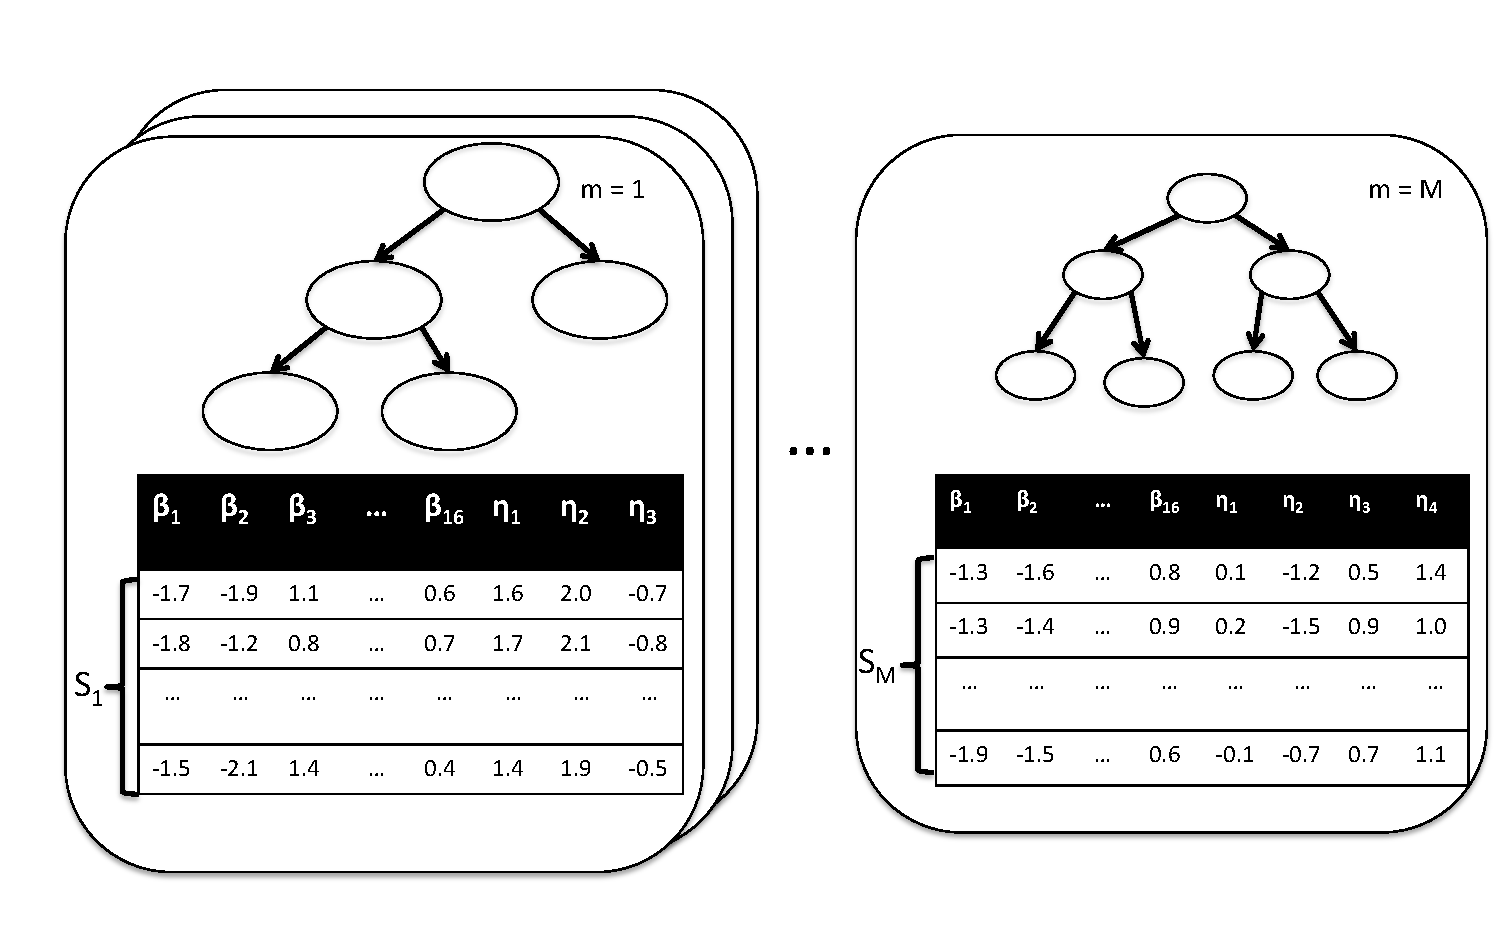
\includegraphics[width=0.75\textwidth]{chapter4/images/sampling_schema}
\caption{Procedural diagram of bayesian model trees}
\label{fig:sampling-process}
\end{figure}


\subsection{Estimation Methods}
\label{sec:estimation-methods}
The previous subsection reviewed the overall framework, mechanics, and parameters of our proposed bayesian model tree. In this subsection, we detail our estimation techniques. These details are discussed at length because we found estimation of this new model to be a nontrivial challenge, and we want other researchers to be able to replicate and build off our work. Readers who would like to immediately get to the results and `big-picture' discussion may feel free to skip ahead to Section \ref{sec:results-and-discussion}.

Subsection \ref{sec:model-framework}'s formulation of $\theta$ shows that the total number of parameters being estimated depends on the decision tree. In particular, as we change from tree to tree, the number of conjunctive conditions ($D^m$) will vary, and as a result, the dimensionality of the parameter vector will vary. Unfortunately, such changing dimensionality necessitates the use of specialized estimation techniques \citep[p.5]{das_2017_transdimensional}. Of these, the reversible-jump algorithm \citep{green_1995_reversible} is the most common bayesian estimation technique for problems of varying dimensionality, both overall \citep{sisson_2005_transdimensional} and for decision trees in particular \citep{denison_1998_bayesian, wu_2007_bayesian, mohammadi_2016_comment}.

As noted by \citet[p.72-73]{fan_2011_reversible}, efficient reversible-jump algorithms require a way for one to propose parameter values of high posterior probability while switching between parameter spaces of varying dimensions, and creating such proposal mechanisms is not straightforward. Our initial attempts at using a reversible-jump algorithm to estimate our model tree failed because we were unable to devise a good way to propose new choice model parameters when switching from one tree to another. How should we propose new bicycle ASCs when the groups of individuals in each output node are completely different? The creation of an efficient, reversible-jump proposal mechanism for bayesian model trees remains an open problem, and it is one that we would be happy to collaborate with others on.

Given our difficulties with the reversible-jump algorithm, we instead sought an alternative estimation strategy. The approach we settled on was to split the problem into two sub-problems, each of which was more easily solved than the original problem. Specifically, as we noted in Section \ref{sec:how-to-estimate-dtrees}, there are existing methods for performing a bayesian estimation of decision trees. Additionally, one can estimate the parameters of a given choice model using almost all existing bayesian estimation techniques for fixed-dimensional problems. In light of these two facts, we sought to break our model tree estimation into a first step where we estimate the decision trees by themselves and a second step where, conditional on a given decision tree, we estimate the choice models that belong in each output node of the tree. Finally, some procedure would be needed to tie these two estimation tasks together.

To implement this divide-and-conquer approach, our original (and idealized) plan was as follows. First, we would use the techniques of \citet{letham_2015_interpretable} to perform a bayesian estimation of the decision trees. Then, conditional on each tree, we would use the techniques of \citet{braun_2016_scalable} to estimate our mode choice model with varying bicycle ASCs. And lastly, we would use importance sampling to adjust the original posterior distribution of decision trees in light of the information provided by the choice models at the output nodes at each tree. Below, we briefly justify each of these choices.

Beginning with the estimation of the decision trees, we chose to use the techniques of \citet{letham_2015_interpretable} for two reasons. First, their methods were implemented in freely available python scripts, so we would not have to re-invent their techniques. Secondly, their approach requires researchers to specify the possible requirements that can be used in the conjunctive conditions that comprise the decision tree. This specification gives researchers the ability to check for sensible relationships between the explanatory variables and the outcomes of interest. For example, by specifying the regions of parameter space that the travel distance is split into, the researcher can empirically check whether the fraction of individuals bicycling decreases as one moves from the region where travel distance is between 2 and 3 miles to the region where travel distance is between 3 and 4 miles.

Moving to the choice model estimation, we (again) had two reasons for choosing the techniques of \citet{braun_2016_scalable}. First, unlike typical MCMC procedures that only generate dependent samples from the posterior distribution of one's choice model parameters, the techniques of \citet{braun_2016_scalable} generate independent samples, resulting in higher effective sample sizes per unit of computational time. Secondly, the methods of \citet{braun_2016_scalable} automatically provide accurate estimates of the total probability of the data given one's decision tree (i.e. after marginalizing over the parameters in the choice model). This probability is needed for our last step: importance sampling.

After the initial estimation of the decision trees and the mode choice models, conditional on the decision trees, we need to link these two estimation procedures. In particular, we want a sample from the joint distribution of decision trees and their accompanying choice models. However, our original sample of decision trees was produced without using any information from the choice models at the output nodes. As a result, our original sample of decision trees is (in general) drawn from an incorrect distribution. We use importance sampling \citep{gelman_1992_iterative, hesterberg_1995_weighted} to weight our original sample of decision trees such that the weighted sample comes from our desired distribution. Since our original sample was drawn from a distribution $P \left( \textrm{tree without choice models} \mid \textrm{data} \right)$ instead of $P \left( \textrm{tree with choice models} \mid \textrm{data} \right)$, we will weight each tree by the ratio $\tfrac{P \left( \textrm{tree with choice models} \mid \textrm{data} \right)}{P \left( \textrm{tree without choice models} \mid \textrm{data} \right)}$. The probabilities in the numerator and denominator are computed up to a constant of proportionality using Bayes rule, and then the importance weights are normalized such that they sum to one across all the trees in our sample. At this point, estimation is complete and the weighted sample is then available for prediction or further inference tasks.

As just described, this three step procedure is our current, ideal method for estimating bayesian model trees. However, this procedure is computationally expensive. For example, our initial sample of trees contained more than 5,000 unique decision trees. On average, for a single decision tree, it took approximately 2 hours to perform the bayesian estimation of the choice models at the output nodes. The total estimation time would have taken more than a week for our dataset and choice model specification (described in Section \ref{sec:data-and-specification}). Given our current computing resources (a single laptop), we deemed this estimation time unreasonable, so we made further approximations to speed up the estimation process. In particular, we selected a subset of 10 decision trees from the total set of unique trees so that the total estimation time would be less than a day. Then, we then estimated the choice models at the output nodes of these trees, and we proceeded as if these ten trees were the complete set of possible trees for our data. As far as we know, it is impossible to account for the existence of the other trees without performing the estimation of those trees' choice models, which is exactly what we wished to avoid. While numerous ways of choosing the ten trees are possible, we tried to follow the intuition of \citet{breiman_2001_random} who noted that the accuracy of a set of trees ``depends on the strength of the individual tree classifiers and a measure of the dependence between them.'' Specifically, we chose the ten trees as follows. We chose top three trees in terms of their (approximate) log-posterior from step 1, and we also chose the top three trees in terms of their (approximate) log-likelihood from step 1\footnote{Note, we use the term `approximate' because the log-posterior values and log-likelihood values of step 1 do not take into account the choice models at the output nodes of the tree.}. We chose the final four trees by first selecting the trees that had approximately the posterior mean number of output nodes ($D^m$) and then, from the selected trees, choosing the 4 trees with the highest log-posterior. This procedure closely follows the recommendation of \citet{letham_2015_interpretable} for selecting a single decision tree to be a point estimate for the posterior distribution of trees. In the end, our selected trees were all ``strong'' in some way, whether that be high log-likelihoods or high log-posterior values, and across the three selection criteria, the trees were quite different from one another. We will refer to the procedure described in this paragraph as our ``actual'' estimation methodology, whereas the procedures described in the paragraphs above are our ``ideal'' estimation methodology. As we will see in Section \ref{sec:results-and-discussion}, despite our radical simplifications, our actual estimation methodology still produces a model that provides quantitatively more accurate and qualitatively more reasonable inferences than the traditional MNL model.

\subsection{Data and model specification}
\label{sec:data-and-specification}
In the previous subsections, we described our model framework and estimation methods. In this section we describe the data used in our application and the precise specification (i.e. model priors and choice model specification) of our bayesian model trees.

\subsubsection{Data}
\label{subsec:data}
Starting with the data, we are using 1,015 observations from the California Household Travel Survey (\citeyear{california_department_of_transportation_2010-2012_2013}). Each individual in our sample lives in Oakland, Berkeley, or San Francisco, CA, and the observations represent home to work or school commute tours. For level-of-service variables (such as travel time, cost, and distance) we use estimates provided by the San Francisco Metropolitan Transportation Commission (MTC) (\citeyear{san_francisco_metropolitan_transportation_commission_travel_2012}). Basing our set of possible alternatives on the alternatives used by MTC, we classify observations as having traveled via one of eight travel modes. There were three driving modes, each differentiated by the number of passengers: drive-alone, shared-ride with two passengers, and shared-ride with three or more passengers. There were also three transit modes, each differentiated by their access and egress modes: walk-transit-walk (where walking is used for access and egress), drive-transit-walk, and walk-transit-drive. Finally, there were two non-motorized modes: walking and bicycling. For each tour, the travel mode that was used for the longest distance was used as the ``chosen travel mode'' for that tour.

Importantly, one of our uses for non-compensatory rules is to determine whether or not an individual considers bicycling as a travel mode. Accordingly, our decision trees are based on spatial variables and socio-demographics that have been mentioned in reasons why individuals did not consider bicycling. In particular, the trees are based on spatial variables such as distance, roadway slopes, elevation, on-street bicycle infrastructure, speed limits, and socio-demographics such as the number of children. Post-processing of the raw spatial data was done using a novel concept called the zone of likely travel. The main idea is, for each individual, to form a buffer around the shortest path between one's home and work or school. This buffer is constrained to follow the roadway network instead of merely being laid atop of a map, and the buffer is constructed so its perimeter is based on each user's likely, maximum deviation from the shortest path. In other words, the zone should contain the roadways over which one is likely to travel. All spatial variables are then calculated over the roadways in one's zone of likely travel. In general, the details of this post-processing procedure are not related to the main purpose of this chapter, so we will not review them any further. However, we instead encourage interested readers to review the details of this processing in \citet{brathwaite_2018_holy}.

\subsubsection{Model Specification}
Traditionally, when discrete choice modelers talk about model specification, they mean the specification of one's utility functions. However, in a bayesian paradigm, one also needs to specify his/her model priors. These priors are probability distributions that encapsulate the modeler's prior beliefs about the true value of the model parameters. Together with the utility specifications and likelihood function, these specification choices allow for model estimation. Below, we will note each our specifications in turn, starting with the choice model.

Specifically, we specify the systematic utility functions in our choice model as follows:

\begin{equation}
\label{eq:utility-specifications}
\begin{aligned}
V_{DA} &= \beta_{\textrm{travel-time-auto}} \textrm{TravelTime}_{\textrm{DA}} + \beta_{\textrm{autos-per-driver}} \textrm{AutosPerDriver}\\
V_{SR2} &= \textrm{ASC}_{\textrm{shared-ride-2}} + \beta_{\textrm{travel-time-auto}} \textrm{TravelTime}_{\textrm{SR2}} + \beta_{\textrm{autos-per-driver}} \textrm{AutosPerDriver} \\
& \quad + \beta _{\textrm{cross-bay}} \textrm{CrossBay} + \beta _{\textrm{num-kids}} \textrm{NumberKids} + \beta_{\textrm{household-size}} \textrm{HouseholdSize}\\
V_{SR3} &= \textrm{ASC}_{\textrm{shared-ride-3}} + \beta_{\textrm{travel-time-auto}} \textrm{TravelTime}_{\textrm{SR3}} + \beta_{\textrm{autos-per-driver}} \textrm{AutosPerDriver} \\
& \quad + \beta _{\textrm{cross-bay}} \textrm{CrossBay} + \beta _{\textrm{num-kids}} \textrm{NumberKids} + \beta_{\textrm{household-size}} \textrm{HouseholdSize}\\
V_{WTW} &= \textrm{ASC}_{\textrm{walk-transit-walk}} + \beta_{\textrm{travel-time-transit}} \textrm{TravelTime}_{\textrm{WTW}} + \beta_{\textrm{travel-cost-transit}} \textrm{TravelCost}_{\textrm{WTW}}\\
V_{WTD} &= \textrm{ASC}_{\textrm{walk-transit-drive}} + \beta_{\textrm{travel-time-transit}} \textrm{TravelTime}_{\textrm{WTD}} + \beta_{\textrm{travel-cost-transit}} \textrm{TravelCost}_{\textrm{WTD}}\\
V_{DTW} &= \textrm{ASC}_{\textrm{drive-transit-walk}} + \beta_{\textrm{travel-time-transit}} \textrm{TravelTime}_{\textrm{DTW}} + \beta_{\textrm{travel-cost-transit}} \textrm{TravelCost}_{\textrm{DTW}}\\
V_{walk} &= \textrm{ASC}_{\textrm{walk}} + \beta_{\textrm{distance-walk}} \textrm{TravelDistance} _{\textrm{walk}}\\
V_{bike} &= \textrm{ASC}_{\textrm{bike}} + \beta_{\textrm{distance-walk}} \textrm{TravelDistance} _{\textrm{bike}}\\
\end{aligned}
\end{equation}
In the systematic utility equations above, DA means ``drive alone,'' SR2 means ``shared-ride with two passengers,'' SR3 means ``shared-ride with three or more passengers,'' WTW means ``walk-transit-walk,'' WTD means ``walk-transit-drive,'' and DTW means ``drive-transit-walk.'' Though not indicated using subscripts on the variables, all of these systematic utility equations are specific to a given individual.

Next, we note that our specifications above were not made arbitrarily. Travel cost was excluded from the driving alternatives because it was too collinear with the travel time variable to permit estimates that had the correct sign. This is to be expected since MTC calculates both its travel cost and travel time estimates for driving modes as a function of travel distance. Secondly, income and gender are not present in our specifications because it was missing for numerous individuals in our dataset.

Finally, the systematic utility specifications shown in Equation \ref{eq:utility-specifications} are common across both the MNL model and the bayesian model trees used in this chapter. There are only two differences between the systematic utility specification of the MNL and the bayesian model trees. First, as mentioned above, the $ASC _{\textrm{bike}}$ is allowed to differ from output node to output node. In other words, the bayesian model trees replace $ASC _{\textrm{bike}}$ with $\sum _{i=1} ^{D^m} \delta _i ASC _{\textrm{bike}, i}$ where $i$ denotes a particular output node of decision tree $m$ and $\delta_i$ is a dummy variable that indicates whether or not an individual is in output node $i$. Briefly, we note that we do not directly estimate the parameters $ASC _{\textrm{bike}, i} \ \forall i \in \left\lbrace 1, 2, ..., D^m \right\rbrace$. This would correspond to using a \textit{no-pooling} estimator that treats the output nodes as being completely different from one another. Instead, we would rather estimate how different the nodes are from one another. To do this, we use a hierarchical logit estimator (i.e. a \textit{partial-pooling} estimator) \citep{bafumi_2006_fitting, gelman_2006_multilevel, gelman_2014_bayesian} that combines (i.e. pools) information about the overall bicycle preference across output nodes. The $ASC _{\textrm{bike}, i}$ parameters are conceptualized as instances from an overall, normal distribution of bicycle ASCs with mean $ASC _{\textrm{bike}}$ and variance $\sigma _{\textrm{bike}} ^2$. Here, the mean and variance parameters are estimated along with the individual $ASC _{\textrm{bike}, i}$ parameters\footnote{To tie this paragraph back to Section \ref{sec:model-framework} where we first discussed our model parameters,  we define $ASC _{\textrm{bike}, i} = ASC _{\textrm{bike}} + \eta _i$. In our application we actually estimate $\eta _i$ and $ASC _{\textrm{bike}}$ instead of $ASC _{\textrm{bike}, i}$ and $ASC _{\textrm{bike}}$. In the statistical literature, this choice is referred to as the use of a non-centered parametrization \citep{papaspiliopoulos_2007_general}. We used the non-centered parametrization instead of the traditional approach of directly estimating $ASC _{\textrm{bike}, i}$ because this method led to faster estimation times.}. As $\sigma _{\textrm{bike}} ^2 \rightarrow \infty$, we are increasingly certain that the output nodes are completely different from one another, and as $\sigma _{\textrm{bike}} ^2 \rightarrow 0$ we are increasingly confident that the general preference for bicycling is actually the same across output nodes.

The second difference is, as noted in Section \ref{subsec:data}, that we use spatial variables in the construction of the decision trees. In order to fairly compare the MNL and the bayesian model tree, we include the spatial variables in the MNL model by placing these variables in the bicycle systematic utility. In particular, the bicycle utility of the MNL model is expanded to include the following variables and their coefficients: shortest path length, median slope, average speed limit, proportion of roadway miles on the shortest path with speed limits of 25 mile per hour or less, proportion of roadway miles with bicycle lanes, and the proportion of roadway miles with ``share the road'' markings (also known as ``sharrows''). These variables are excluded from the bicycle utility of the choice models in the bayesian model tree as they are already used when constructing the decision trees.

Next we state our model priors. In a bayesian setting, priors must be specified for all parameters that are being estimated. We start with the choice model parameters. For all choice model parameters, excluding $ASC _{\textrm{bike}, i} \ \forall i  \in \left\lbrace 1, 2, ..., D^m \right\rbrace$ and $\sigma _{\textrm{bike}} ^2$, we assumed independent priors of $\mathcal{N} \left( 0, 4 \right)$ where 4 is the variance of the normal distribution. This prior was chosen to reflect the fact that we think it is highly unlikely for a 1-unit change of any of our variables to cause a change of 4 in our systematic utility functions. Such changes would greatly increase or decrease the probability of choosing a given alternative, and we don't expect a 1 minute change in travel time, a 1 dollar change in travel cost, a change in 1 mile of travel distance, etc. to cause drastic changes in the probability of a given mode. For, the $ASC _{\textrm{bike}, i}$ parameters, we use the prior distribution mentioned above. That is, the prior distribution of $ASC _{\textrm{bike}, i}$ is $\mathcal{N} \left( \textrm{ASC}_{\textrm{bike}}, \sigma _{\textrm{bike}} ^2 \right)$. Here, we again use a $\mathcal{N} \left( 0, 4 \right)$ for the hyperprior on $ASC _{\textrm{bike}}$. The hyperprior for the variance is specified as $\ln \left[ \mathcal{N} \left( 0, 4 \right) \right]$, i.e. log-normal with a location parameter of zero and a scale parameter of 2 ($\sqrt{4} = 2$).

Moving to our priors for the parameters of the model trees, we need a prior distribution for $\left( D^m, \mid p_i ^m \mid, b_j ^{i, m} \right)$ for all $i \in \left\lbrace 1, 2, ..., D^m \right\rbrace$ and for all $j \in \left\lbrace 1, 2, ..., \mid p_i ^m \mid \right\rbrace$. To construct our prior, we precisely follow the methodology described in Section 2 of \citet{letham_2015_interpretable}. Unfortunately, this methodology took \citeauthor{letham_2015_interpretable} nearly four pages and much mathematical notation to describe. Additional pages would be needed to relate their original description to the characterization of decision trees that we have given in Sections \ref{sec:decision-tree-explanation} and \ref{sec:decision-tree-economics}. Since reviewing the techniques of \citet{letham_2015_interpretable} is not a primary focus of our article, we state upfront that the following description of our prior distribution of decision trees will be necessarily brief and will likely require a reader to consult \citet{letham_2015_interpretable} for full understanding. For readers who prefer reading code to reading verbal descriptions of our procedures, all scripts used in this application are available upon request.

Now, we begin with $D^m$, the number of output nodes (or conjunctive conditions) in our decision tree. Given that one of the arguments for non-compensatory rules is that humans are boundedly rational and only spend but so much mental effort making decisions, we do not think individuals are using overly complex rules. Our prior for $D^m$ was therefore specified as a truncated Poisson distribution with a rate parameter of 5, reflecting our prior belief that the expected number of output nodes in one's decision tree is approximately five. A truncated (as opposed to standard) Poisson distribution was used because the support of the standard Poisson distribution extends to positive infinity whereas the number of possible conjunctive conditions for the trees is limited by the finite number of possible requirements from which the conjunctive rules can be composed. See \citet[p. 1355]{letham_2015_interpretable} for the specific form of the truncated Poisson distribution and for more details on this prior specification.

Continuing to the next parameter, we have to specify a prior for $\mid p_i ^m \mid$: the number of requirements in each conjunctive condition. We will not delve into the details here, but the methods of \citet{letham_2015_interpretable} use a slightly different representation of decision trees than have been described in this chapter. In their formulation, output nodes are evaluated sequentially, and $\mid p_i ^m \mid$ represents the number of requirements in output node $i$, conditional on the requirements of the previous nodes not being met. Given this set up, and given the assumption that people are using relatively simple rules to make their decisions, we specify our prior for $\mid p_i ^m \mid$ as a truncated Poisson distribution with a rate parameter of 2. In other words, besides the requirement of not meeting the conditions specified by the previous output nodes, we expect that a given output node will be described by approximately two requirements.

Next, we need prior distributions for the requirements ($b_j ^{i, m}$) that make up each conjunctive condition. We pause here to note that such prior distributions implicitly define a prior on the conjunctive conditions ($p_i$) that correspond to each output node. Alternatively, placing a prior directly on the conjunctive conditions ($p_i$) will implicitly define a prior on the requirements ($b_j ^{i, m}$) that make up these conditions. Following the procedures in \citet{letham_2015_interpretable}, we use a three-stage procedure to place a prior directly on the conjunctive conditions ($p_i$). First, we specify the possible requirements that a conjunctive condition can be composed of. These requirements are formed by discretizing the explanatory variables into various ranges (e.g. minimum distance greater than 4 miles). Second, we specify which of the possible combinations of requirements will be allowed as possible conjunctive conditions. And finally, we specify a prior distribution over the possible conjunctive conditions. We will discuss each of these three steps below.

To specify the possible requirements from which a conjunctive condition could be composed, our strategy\footnote{Note, we are aware that other strategies could have been used to discretize our variables in order to create requirements for use in the decision tree. Future researchers are free to use any such discretization strategies they prefer and to make a case for such strategies. We chose to follow the procedures of \citet{letham_2015_interpretable} who manually discretized their variables according to their a-priori beliefs.} was to subdivide the explanatory variables used to construct the decision tree into as many equal sized groups as possible. The only constraint was that the partition had to maintain the expected relationships between the groups and the outcome of bicycling or not. For example, the variable denoting the number of children was split into three groups: $\left[ 0, 1 \right]$, $\left( 1, 2 \right]$, and $\left( 2, \infty \right)$. For these categories of the number of children, the percentages of individuals in each category that owned a bicycle and actually bicycle to work or to school were approximately 16\%, 13\% and 0\%. Such trends follow our a-priori expectations that the probability of bicycling decreases as one has more children. Sub-dividing the number of children variable into 4 or more categories led to relationships that were deemed to be spurious since they did not match our a-priori beliefs about the relationship between number of children and the probability of bicycling commuting. All together, the possible requirements used to construct the decision tree were as follows (with numbers rounded to two decimal places, or more when necessary):
\begin{itemize}
\item Number of Kids: $\left[ 0, 1 \right]$, $\left[ 2 \right]$, and $\left[ 3, \infty \right)$

\item Minimum distance (miles): $\left[ 0, 1.17 \right]$, $\left( 1.17, 1.92 \right]$, $\left( 1.92, 3.00 \right]$, $\left( 3.00, 4.37 \right]$, $\left( 4.37, \infty \right)$

\item Average Speed Limit (miles per hour): $\left[ 23.01, 25.15 \right]$, $\left( 25.15, 25.78 \right]$, $\left( 25.78, \infty \right)$

\item Median Slope (meters per foot): $ \left[0, 0.01 \right]$, $\left( 0.01, 0.02 \right]$, $\left( 0.02, 0.03 \right]$, $\left( 0.03, 0.04 \right]$, $\left(0.04, \infty \right)$

\item Proportion of roadway miles along one's shortest path with speed limits $<$ 25 miles per hour: \newline $\left[ 0, 0.66 \right]$, $\left( 0.66, 0.83 \right]$, $\left( 0.83, 0.95 \right]$, $\left( 0.95, 0.9984 \right]$, $\left( 0.9984, 0.9986 \right]$, $\left( 0.9986, \infty \right)$

\item Proportion of roadway miles with bicycle lanes: $\left[ 0, 0.04 \right]$, $\left(0.04, 0.11 \right]$, $\left( 0.11, \infty \right)$

\item Proportion of roadway miles with ``share the road'' markings: $\left[ 0, 0.08 \right]$, $\left(0.08, 0.14 \right]$, $\left( 0.14, \infty \right)$

\end{itemize}
These requirements are all binary boolean conditions that are to be read as ``\textit{variable} in \textit{range}.'' For instance, ``minimum distance in [0, 1.17].'' 

Given the possible requirements specified above, the next task is to specify the combinations of these requirements that will be allowed as possible conjunctive conditions in our decision trees. Going along with the notion of non-compensatory rules are at least partially motivated by a desire to minimize cognitive effort, we hypothesize that no individual conjunctive condition will be made up of a large number of requirements. As a result, we specify the maximum number of requirements in a conjunctive condition to be 2. Moreover, since we are trying to estimate a decision tree that (by assumption) is used by our entire population, we limit the possible conjunctive conditions to those conjunctions that apply to a large percentage of the population. In particular, we only consider those conjunctive conditions that apply to (1) 10\% or more of those who bicycle or (2) 10\% or more of those who did not bicycle. As is done in \citet{letham_2015_interpretable}, we use the FP-growth algorithm implemented by \citet{borgelt_2005_implementation} to enumerate these conjunctive conditions.

Now, given the possible conjunctive conditions, our remaining task is to assign a prior probability to each of these conjunctive rule. Because we do not have any prior information about whether one conjunctive condition would be used more than any other, we use a uniform distribution as our prior. In particular, we follow Equation 2.2 of \citet{letham_2015_interpretable} and place a uniform distribution prior over all conjunctive conditions that (1) have $\mid p_i ^m \mid$ requirements and (2) have not already been used in the decision tree.

Lastly, in order to use the methods of \citet{letham_2015_interpretable}, we initially use the decision trees to predict the choice of bicycling or not, for those individuals who own a bicycle. This bicycle focused prediction is performed for two reasons. First, we are being agnostic (initially) about the presence of a more general choice model at the output nodes of the decision tree, and unlike our mode choice models, our trees are not constructed with the relevant variables for predicting all travel modes. Secondly, we focus on the choice of bicycling because the tree is will ultimately be used specifically to determine whether bicycle is considered or not and to what extent bicycling is generally preferred when it is considered. Either way, to make predictions about whether or not an individual bicycles to work or to school, the methods of \citet{letham_2015_interpretable} require us to specify a prior for the probability that an individual chooses to bicycle. For a fully unknown person, we chose our prior to express maximal ignorance about his/her probability of bicycling. Our prior for the probability that an individual commutes by bicycle is $\textrm{Beta} \left( 1, 1 \right)$: a uniform distribution over the range $\left( 0, 1 \right)$.

For further clarification of how we initially sampled the decision trees, see \citet{letham_2015_interpretable}.
\subsection{Results and Discussion}
\label{sec:results-and-discussion}

In this subsection, we discuss the results of our empirical application. Specifically, we compare the MNL model with our proposed bayesian model trees in four ways. We first quantitatively compare these two models in terms of in-sample fit. Note that we do not compare the two models in terms of out-of-sample predictive ability simply because our long estimation times and small sample size made both cross-validation and the use of a holdout sample unappealing. Moreover, it is well known that while frequentist estimation techniques such as maximum likelihood are prone to over-fitting, bayesian estimation techniques are much less likely to overfit, and bayesian model selection techniques automatically penalize model complexity (\citealp{dawid_2002_comment}; \citealp[Section 3.2]{wagenmakers_2008_bayesian}). Secondly, we qualitatively compare the two models in terms of their forecasted relationship between public investments in bicycle lanes and expected bicycle mode shares. Thirdly, in an attempt to uncover the model differences that lead to the divergent forecasts, we compare the estimation results of those coefficients that are common to the two models. Finally, we conclude this subsection by discussing the behavioral differences that lead to greater plausibility of our bayesian model tree forecasts as compared to the forecasts of the MNL model.

To begin, we start with the in-sample results. In a frequentist setting, models are commonly compared using log-likelihood ratios. For non-nested models, one might use the Vuong test (a generalization of the likelihood ratio test) to test which of two models is closer in terms of Kullback-Leibler divergence to the true data generating process \citep{vuong_1989_likelihood}. In a bayesian setting, the same interpretation can be given to the posterior probability of a model. Simply, the posterior probability of a model is the probability that, out of one's set of models, a given model is closest in terms of Kullback-Leibler divergence to the true data generating process \citep{walker_2013_bayesian}. Because we use the scalable rejection sampling algorithm of \citet{braun_2016_scalable}, we automatically get an estimate of $P \left( Y \mid X, m \right)$ for each of our ten model trees, and because we have the prior of each tree $m$, we can calculate $P \left( Y \mid X \right)$ given our bayesian model tree. Likewise, the scalable rejection sampling algorithm provides an estimate of $P \left( Y \mid X \right)$ for our MNL model. Combining these probabilities with prior probabilities of $\tfrac{1}{2}$ for each model (to reflect maximal uncertainty about which model is closest to the data generating process), we find that the posterior probability of our bayesian model trees is 99.91\% compared to the posterior probability of 0.09\% for the MNL model. In other words, based on our data, the bayesian model tree is overwhelmingly more likely to be closer to the true data generating process than the MNL model.

\begin{figure}
\centering
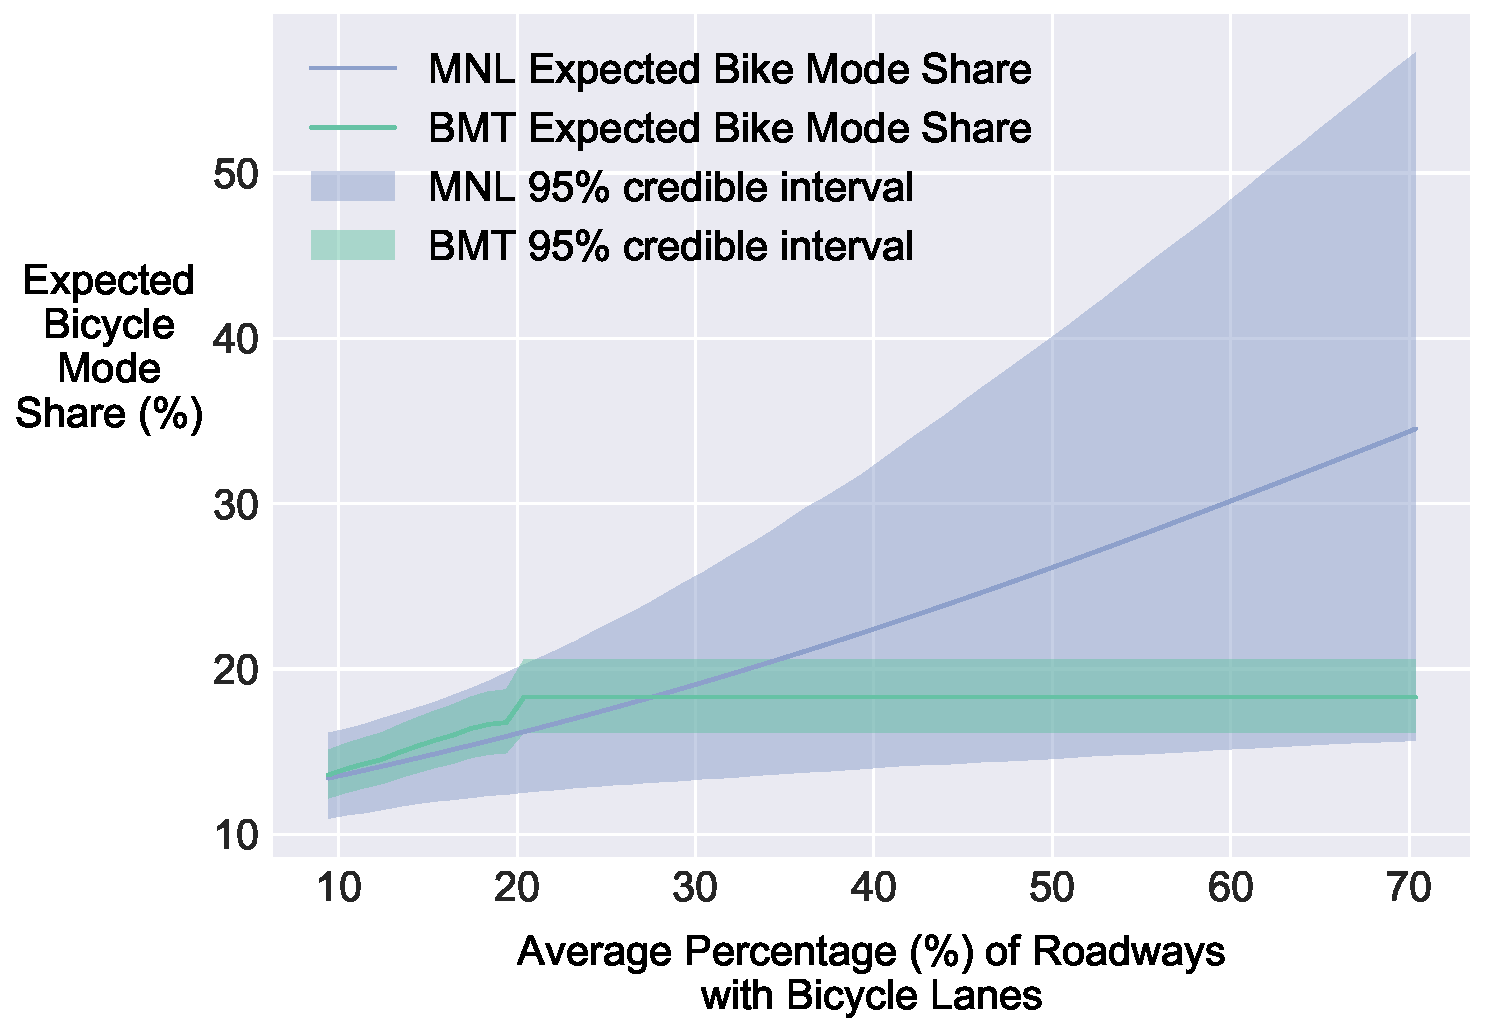
\includegraphics[width=0.7\textwidth]{chapter4/images/bike_mode_share_plot_v3}
\caption{Expected Bicycle Mode Share versus Mean Percentage of Bicycle Lanes}
\label{fig:mode-share-plot}
\end{figure}

Given that the bayesian model trees are likely to be a better representation of the true data generating process, we now turn to the question of whether this model leads to different policy implications as compared to the MNL model. For our policy application, we considered the effect of increasing the proportion of bicycle lanes for the individuals in our sample. In particular, we raised the proportion of bicycle lanes for each individual in our sample, one percentage point at a time, until each individual's proportion of bicycle lanes was approximately 70\% (the maximum value observed in our estimation dataset). After each incremental increase in the proportion of roadways with bicycle lanes, we predicted the average bicycle mode share across the dataset. In Figure \ref{fig:mode-share-plot} we plot the expected bicycle mode shares, as predicted by the bayesian model trees and the MNL model, along with their associated credible intervals\footnote{Note that credible intervals are the bayesian analog of confidence intervals}. Note that in this plot, we use the acronym ``BMT'' to refer to the bayesian model trees. Naming aside, Figure \ref{fig:mode-share-plot} shows that the two models lead to very different forecasts. In particular, as one begins to install bicycle lanes, both models show an increase in the expected bicycle mode share, but eventually, the bayesian model trees predicts that the expected bicycle mode share will flatline. In contrast, the MNL model predicts that the expected bicycle mode share will increase continually. A-priori, the predictions of the bayesian model trees appear more plausible than the predictions of the MNL model. In particular, we expect diminishing returns from increasing the proportion of roadways with bicycle lanes since individuals will eventually come to feel safe on public roadways but will still reject the bicycling alternative due to other factors such as time pressures due to childcare obligations, concerns about sweating, etc.

To corroborate our a-priori expectations, we note that in the United States (U.S.) and internationally, solely having many bicycle lanes does not lead to the huge bicycle mode shares predicted by the MNL model. For instance, take the case of Davis, California. Davis has lead the U.S. in the installation of on-street bicycle infrastructure. The first on-street bicycle lanes, the first bicycle traffic signal, and the first `protected intersection' for bicyclists were all installed in Davis \citep{caltrans_2017_toward}. Accordingly, out of all cities in the U.S. with populations of greater than 20,000 individuals, Davis has the highest bicycle commuting mode share. Depending on one's source, Davis' bicycle commuting mode share is 17\% - 19\% \citep{mckenzie_2014_modes, mcleod_2016_where}, a value that precisely matches the predictions of our bayesian model trees. Looking internationally, we can observe countries such as the Netherlands that lead the world in on-street bicycle infrastructure investments. Here, we are quick to note that bicycle infrastructure in the Netherlands is often of much higher quality than in the U.S. Bike lanes in the Netherlands are often `protected' in the sense that they are physically-separated from motor vehicles \citep{pucher_2008_making}. Additionally, the entire travel context in the Netherlands is more supportive of bicycling: fuel and automobile-ownership costs are much higher than in the U.S., more downtown areas are designated as automobile-free, local roads are often `traffic-calmed,' and travel by bicycle is often more direct than by automobile \citep{pucher_2008_making}. Even with all of these advantages, only about 36\% percent of all trips are taken by bicycle in the Netherlands \citep{directorate_2015_quality}. We are immediately sceptical of any model, such as our MNL model, that predicts a similar level of bicycling based solely on the installation of `unprotected' bicycle lanes (the only type of bicycle lane present in our study area at the time the data was collected).

Now, to investigate the causes of the differing forecasts shown in Figure \ref{fig:mode-share-plot}, we start with the estimated choice model coefficients ($\beta$) of the MNL model and our bayesian model trees. A summary of the posterior distribution of the choice model parameters for both the MNL and bayesian model trees is given in Table \ref{table:posterior-summaries}. Briefly, Table \ref{table:posterior-summaries} shows the posterior mean, the 2.5th percentile, and the 97.5th percentile of the posterior samples for each choice model parameter. To calculate the posterior summary for the bayesian model trees, we calculated a weighted posterior mean and weighted percentiles where the posterior samples of each choice model parameter, for each decision tree, were weighted by the posterior probability of that tree. To make the display manageable, Table \ref{table:posterior-summaries} only displays the parameters estimated in the MNL model. The parameters that are specific to the model trees, such as the bicycle ASCs that are specific to each output-node ($\textrm{ASC}_{\textrm{bike}, i}$), are not shown. Now, the main finding from Table \ref{table:posterior-summaries} is that the estimation results of parameters that are common to both models are very similar. The only parameter whose posterior mean shows large differences between the two models is $\textrm{ASC}_{\textrm{bike}}$, and this is because the $\textrm{ASC}_{\textrm{bike}}$ in the bayesian model tree plays a different role than it does in the MNL model. Recall that in the bayesian model tree, $\textrm{ASC}_{\textrm{bike}}$ is just the group mean that the output-node specific $\textrm{ASC}_{\textrm{bike}, i}$ are centered around. Details aside, knowing that the estimated choice models are the largely the same means that we should look towards the decision trees themselves to find out why the two models have such differing forecasts. This line of investigation is pursued below.

Behaviorally, we believe that four qualities of our bayesian model trees lead to its differing forecasts from the MNL model. The first quality we note is that the bicycle lane variable is almost never included in the conjunctive condition that splits the root node. In other words, the bicycle lane variable is almost never in the conditions at the top of our decision trees. In nine of our ten decision trees, there were nodes that filtered out individuals before they could get to an output node that depended on bicycle lanes. Furthermore, the one tree that had a bicycle lane requirement for the first output node actually had a low probability (0.2\%) of being the tree that is closest to representing the true data generating process. The behavioral interpretation of this finding is that bicycle lanes are not the most important variable in an individual's decision making process about whether or not to commute by bike. Variables that appear to take precedence over bicycle lanes when deciding whether or not to commute by bike include topography, the number of children an individual has, and the minimum distance between an individual's home and work/school. As a result, the impact of installing bicycle lanes will be moderated by these other variables.

The second quality that we note about our bayesian model trees is that the bicycle lane variable never appeared by itself. In particular, when the proportion of roadways containing bicycle lanes was present in a conjunctive condition, it always appeared alongside another variable. For instance, in seven out of ten decision trees, the bicycle lane variable appeared in the following conjunctive condition: `proportion of roadways with bicycle lanes is greater than 0.11 and the number of children is 0 or 1.' The posterior probability that the true data generating process was most closely represented by one of these seven trees was over 99\%. Such a finding emphasizes that the proportion of roadways containing bicycle lanes is not always important. In particular, if a person has 2 or more children, then bicycle lanes are unlikely to affect whether the individual commutes by bicycle. Presumably, childcare pressures will be a bigger determining factor of those individuals' choice of travel mode.

\begin{landscape}
\begin{table}
\centering

\caption{Posterior Summaries of Choice Model Parameters}
\label{table:posterior-summaries}

\begin{tabular}{K{0.45\linewidth}rrrrrr}
\toprule
{} & \multicolumn{3}{c}{MNL} & \multicolumn{3}{c}{Bayesian Model Trees}\\
Variables & \multicolumn{1}{c}{Mean} & \multicolumn{1}{c}{2.5\%} & \multicolumn{1}{c}{97.5\%} & \multicolumn{1}{c}{Mean} & \multicolumn{1}{c}{2.5\%} & \multicolumn{1}{c}{97.5\%} \tabularnewline
\midrule

\multicolumn{7}{l}{Alternative Specific Constants}\\
\quad Shared Ride: 2 & -1.746*\hphantom{*} & -2.282 & -1.231 & -1.787*\hphantom{*} & -2.322 & -1.259\\
\quad Shared Ride: 3+ & -1.865*\hphantom{*} & -2.378 & -1.345 & -1.909*\hphantom{*} & -2.453 & -1.378\\
\quad Walk-Transit-Walk & 1.070*\hphantom{*} & 0.495 & 1.623 & 1.078*\hphantom{*} & 0.497 & 1.666\\
\quad Drive-Transit-Walk & -2.183*\hphantom{*} & -2.969 & -1.431 & -2.223*\hphantom{*} & -3.060 & -1.418\\
\quad Walk-Transit-Drive & -2.677*\hphantom{*} & -3.537 & -1.886 & -2.734*\hphantom{*} & -3.602 & -1.910\\
\quad Walk & 2.428*\hphantom{*} & 1.826 & 3.042 & 2.504*\hphantom{*} & 1.885 & 3.149\\
\quad Bike & 1.087\hphantom{*}\hphantom{*} & -2.573 & 4.854 & 0.171\hphantom{*}\hphantom{*} & -3.419 & 3.738\\

\multicolumn{7}{l}{Travel Time, units:0.1min}\\
\quad All Auto Modes & -1.113*\hphantom{*} & -1.358 & -0.875 & -1.129*\hphantom{*} & -1.383 & -0.894\\
\quad All Transit Modes & -0.374*\hphantom{*} & -0.479 & -0.273 & -0.378*\hphantom{*} & -0.486 & -0.276\\

\multicolumn{7}{l}{Travel Cost, units:\$}\\
\quad All Transit Modes & -0.173*\hphantom{*} & -0.300 & -0.053 & -0.173*\hphantom{*} & -0.301 & -0.048\\

\multicolumn{7}{l}{Travel Distance, units:mi}\\
\quad Walk & -1.125*\hphantom{*} & -1.299 & -0.960 & -1.151*\hphantom{*} & -1.337 & -0.979\\
\quad Bike & -0.242\hphantom{*}\hphantom{*} & -0.503 & 0.052 & -0.356*\hphantom{*} & -0.469 & -0.245\\

\multicolumn{7}{l}{Systematic Heterogeneity}\\
\quad Autos per licensed drivers (All Auto Modes) & 1.181*\hphantom{*} & 0.784 & 1.582 & 1.221*\hphantom{*} & 0.822 & 1.621\\
\quad Cross-Bay Tour (Shared Ride 2 \& 3+) & -0.517\hphantom{*}\hphantom{*} & -1.264 & 0.167 & -0.518\hphantom{*}\hphantom{*} & -1.286 & 0.201\\
\quad Household Size (Shared Ride 2 \& 3+) & 0.108\hphantom{*}\hphantom{*} & -0.097 & 0.311 & 0.127\hphantom{*}\hphantom{*} & -0.079 & 0.330\\
\quad Number of Kids in Household (Shared Ride 2 \& 3+) & 0.662*\hphantom{*} & 0.414 & 0.903 & 0.634*\hphantom{*} & 0.394 & 0.892\\

\multicolumn{7}{l}{Spatial Variables}\\
\quad Minimum Distance units:mi (Bike) & -0.232\hphantom{*}\hphantom{*} & -0.822 & 0.294 & \_ & \_ & \_\\
\quad Median Slope units:m/ft (Bike) & -1.433\hphantom{*}\hphantom{*} & -5.046 & 2.304 & \_ & \_ & \_\\
\quad Mean Speed Limit units:mph (Bike) & -0.064\hphantom{*}\hphantom{*} & -0.206 & 0.072 & \_ & \_ & \_\\
\quad Proportion of Shortest Path Roads slower than 25mph (Bike) & 0.484\hphantom{*}\hphantom{*} & -0.701 & 1.791 & \_ & \_ & \_\\
\quad Proportion of Roadways with Bike Lanes (Bike) & 2.218*\hphantom{*} & 0.363 & 4.048 & \_ & \_ & \_\\
\quad Proportion of Roadways with Bicycle Chevrons (Bike) & -0.765\hphantom{*}\hphantom{*} & -2.647 & 1.108 & \_ & \_ & \_\\


\bottomrule
\multicolumn{7}{l}{Note: * means the equal-tailed 95\% credible interval excludes zero.}\tabularnewline
\multicolumn{7}{l}{\qquad \hphantom{*} Additionally, bicycle chevrons are another name for ``share the road'' arrows.}
\end{tabular}

\end{table}
\end{landscape}

Third, we point out that decision trees, by their very nature, incorporate a notion of threshold effects. These threshold effects can be seen in our application by the fact that all of our decision trees with posterior probabilities of greater than 0.2\% all feature the requirement that the `proportion of roadways with bicycle lanes is greater than 0.11.' Undoubtedly, the presence of this sharp discontinuity at 0.11 is partly an artifact of our discretization methods. However, as described in Section \ref{sec:dtree-variants-heterogeneity}, even when using soft decision trees that don't implement such ``hard'' thresholds, the interpretation is that individuals do use hard thresholds, but we are merely uncertain about what those hard thresholds are. Either way, the presence of these threshold effects leads to two features of our forecasts. First, the threshold effects lead to the discrete jump in the expected bicycle mode share when the average percentage of all roadways containing bicycle lanes is about 20\%. At this point, almost everyone's proportion of roadways with bicycle lanes rises above 0.11, so all individuals now belong to output nodes with the highest chance of bicycling. Secondly, the threshold effects also cause the flatline in expected bicycle mode share. Because further increases in the proportion of roadways with bicycle lanes do not cause any more changes in the output node's of an individual, there are no more changes in the probability that an individual chooses to bike.

Finally, the last major difference between the forecasts of the bayesian model trees and the MNL model is that as the average percentage of roadways with bicycle lanes increases, the variance in the expected bicycle mode share increases for the MNL model but not for the bayesian model trees. This finding is perhaps best explained mathematically. Whether operating in a frequentist or bayesian setting, the parameters of one's choice model will have an associated probability distribution. In a frequentist setting, this will be the sampling distribution of $\hat{\beta}$ and in a bayesian setting, this will be the posterior distribution of $\beta$. For ease of exposition, we will continue our discussion from a bayesian perspective, but our explanation is equally valid from a frequentist perspective. Since the MNL model multiplies the proportion of roadways with bicycle lanes ($X_{\textrm{bike-lanes}}$) by $\beta_{\textrm{bike-lanes}}$, we can calculate the variance of the product as $\textrm{Var}  \left[ X_{\textrm{bike-lanes}} \beta_{\textrm{bike-lanes}} \right] = X_{\textrm{bike-lanes}} ^2 \textrm{Var}  \left[ \beta_{\textrm{bike-lanes}} \right]$. This means that as $X_{\textrm{bike-lanes}}$ increases, the variance of $X_{\textrm{bike-lanes}} \beta_{\textrm{bike-lanes}}$ increases. Because the MNL's probability that an individual commutes by bicycle is dependent on $X_{\textrm{bike-lanes}} \beta_{\textrm{bike-lanes}}$, the increase in the variance of $X_{\textrm{bike-lanes}} \beta_{\textrm{bike-lanes}}$ leads to an increase in the variance of the probability that an individual commutes by bicycle. Aggregated over all individuals, the increases in the variances of the bicycle probabilities lead to an increase in the variance of the expected bicycle mode share.

In contrast to the process described above, changing the value of $X_{\textrm{bike-lanes}}$ when forecasting with the bayesian model trees only changes what output node one falls into for a given decision tree. The structure of the trees remains unchanged, the posterior probabilities across the trees remains unchanged, and the variance of the $\textrm{ASC}_{\textrm{bike}, i}$ remain mostly constant across output nodes that have bicycle available as an alternative. As a result, the variance of the expected bicycle mode share remains mostly constant as $X_{\textrm{bike-lanes}}$ is increased for the various individuals in our dataset. Behaviorally, these differences in forecast uncertainty can be attributed to the fact that when using a compensatory model, one is uncertain about the extent to which the proportion of roadways with bicycle lanes compensates for the other variables that affect one's probability of bicycling. In other words, one is uncertain about the value of $\hat{\beta}_{\textrm{bike-lanes}}$ or $\beta_{\textrm{bike-lanes}}$. Since $X_{\textrm{bike-lanes}}$, only appears in the non-compensatory portion of our bayesian model trees (i.e. in the decision trees as opposed to the choice model), we are always certain that the bike lane proportion does not compensate for other variables. I.e. our bayesian model trees are based on the assumption that $\beta_{\textrm{bike-lanes}} = 0$. This constant level of uncertainty with respect to the compensatory nature of $X_{\textrm{bike-lanes}}$ leads directly to the constant level of forecast uncertainty for the bayesian model trees in Figure \ref{fig:mode-share-plot}.

\section{Conclusion}
\label{sec:conclusion}
In this chapter, we have made three contributions to the literature. First, we have provided a micro-economic framework for interpreting a class of machine learning models known as decision trees. In particular, we reviewed how decision trees are used and estimated (Section \ref{sec:decision-tree-explanation}), we showed how decision trees represent a non-compensatory decision protocol known as disjunctions-of-conjunctions (Section \ref{sec:decision-tree-economics}), and we discussed how existing decision tree variants can account for economic considerations that discrete choice modelers are likely to have (Section \ref{sec:decision-tree-variants}).

Secondly, we contributed to both the discrete choice and decision tree literatures by formulating and estimating the first bayesian model tree for discrete choice problems. The result is a semi-compensatory, two-stage model of human decision making. Our model uses a non-compensatory, disjunctions-of-conjunctions protocol to determine one's choice set, and conditional on a given choice set, it uses a compensatory discrete choice model (e.g. an MNL model) to make a final selection if more than one alternative is available. Beyond one's choice set, our bayesian model tree allows the non-compensatory rules to influence one's preferences, as embodied in the choice model parameters, and our model allows for quantification of one's uncertainty over which set of disjunctions-of-conjunctions are actually being used in a population. To the best of our knowledge, this is the first time a bayesian model tree has ever been proposed and estimated for discrete choice problems.

Finally, beyond the mere proposition of the bayesian model tree, this chapter carried out an empirical application of this model. We made three major findings. First, our proposed bayesian model tree is more than 1,000-times more likely ($\frac{99.01}{0.09} \approx 1,100$) to be closer to our application's true data-generating process than the MNL model. Second, our bayesian model trees provide forecasts that are consistent with observed bicycle mode shares in areas with abundant bike lanes such as Davis, CA and the Netherlands. In comparison, the forecasts of the MNL model were overly optimistic. Third, our bayesian model trees provide insights that are qualitatively different than the MNL model. Specifically, our bayesian model trees suggest that (1) investments in on-street bicycle lanes will eventually suffer from diminishing returns and (2) that factors such as travel distance, child-related pressures, and topography may all prevent individuals from bicycling even if there are many bicycle lanes. These insights are missing from the more traditional (and compensatory) MNL model.

Moving forward, we note that in the decades after McFadden revealed the economic implications of the conditional logit model, discrete choice modelers moved swiftly to create needed extensions. As a result, we can now avoid many of the troubling assumptions and properties of the conditional logit model, leading to more accurate analyses and more sensible policy implications. Analogously, by linking decision trees to economics, this chapter brings decision trees to a similar, infantile stage. As noted in Section \ref{sec:dtree-combinatorics}, there remain a number of economic concerns (or more specifically, combinations of concerns) that must be confronted before decision trees will be maximally useful in policy settings. By detailing the microeconomic implications of decision trees, we aim to draw the attention of choice modelers. Hopefully, this chapter will encourage the use and extension of current decision tree methodologies, thereby increasing the accuracy and usefulness of such models for policy analyses.

\section{Acknowledgements}
We thank Paul Waddell, the MacArthur Foundation, and UCCONNECT's Dissertation Grant for funding this research. We also thank Feras El Zarwi, Sreeta Gorripaty, and Madeleine Sheehan for their helpful discussions in the beginning stages of this research endeavor.

\newpage
\renewcommand\bibname{{References}} %  will print ''REFERENCES'' instead of ''BIBLIOGRAPHY''
\bibliographystyle{plainnat}
\bibliography{chapter4/current/ch4}

%\clearpage
%!TEX root = chapter5/../dissertation.tex

\chapter{Causal Inference in Travel Demand Modeling (and the lack thereof)}
\label{ch:5}

\begin{chapterabstract}
This chapter is about the general disconnect that we see, both in practice and in literature, between the disciplines of travel demand modeling and causal inference. In this chapter, we assert that travel demand modeling should be one of the many fields that focuses on the production of valid causal inferences, and we hypothesize about reasons for the current disconnect between the two bodies of research. Furthermore, we explore the potential benefits of uniting these two disciplines. We consider what travel demand modeling can gain from greater incorporation of techniques and perspectives from the causal inference literatures, and we briefly discuss what the causal inference literature might gain from the work of travel demand modelers. In this chapter, we do not attempt to ``solve'' issues related to the drawing of causal inferences from travel demand models. Instead, we hope to spark a larger discussion both within and between the travel demand modeling and causal inference literatures. In particular, we hope to incite discussion about the necessity of making causal inferences in travel demand applications and the methods by which one might credibly do so.
\end{chapterabstract}

\section{What demand modelers have always wanted to do}
\label{sec:travel_demand_goals}
Consider the following three quotations.
\begin{quotation}
``Travel demand models are used to aid in the evaluation of alternative policies. The purpose of the models is to predict the consequences of alternative policies or plans. [...] Predictions made by the model are conditional on the correctness of the behavioral assumptions and, therefore, are no more valid than the behavioral assumptions on which the model is based. A model can duplicate the data perfectly, but may serve no useful purpose for prediction if it represents erroneous behavioral assumptions. For example, consider a policy that will drastically change present conditions. In this case the future may not resemble the present, and simple extrapolation from present data can result in significant errors. However, if the behavioral assumptions of the model are well captured, the model is then valid under radically different conditions.''  ---\citep{ben1973structure}
\end{quotation}

\begin{quotation}
``Indeed, causal models (assuming they are valid) are much more informative than probability models. A joint distribution tells us how probable events are and how probabilities would change with subsequent observations, but a causal model also tells us how these probabilities would change as a result of external interventions---such as those encountered in policy analysis, treatment management, or planning everyday activity. Such changes cannot be deduced from a joint distribution, even if fully specified.'' ---\citep{pearl2009causality}
\end{quotation}

\begin{quotation}
``The goal of many sciences is to understand the mechanisms by which variables came to take on the values they have (that is, to find a generative model), and to predict what the values of those variables would be if the naturally occurring mechanisms were subject to outside manipulations. [...] Finding answers to questions about the mechanisms by which variables come to take on values, or predicting the value of a variable after some other variable has been manipulated, is characteristic of causal inference.''---\citep{spirtes2010introduction}
\end{quotation}

Based on personal communication with many travel demand modelers, i.e. based on anecdote, we believe that the first quotation, by Moshe Ben-Akiva, accurately represents the opinions of most researchers and practitioners within the field of transportation. Moreover, we think it is safe to say that a ``policy that will drastically change present conditions'' can be categorized as an ``external intervention'' or ``outside manipulation.'' If one accepts these two premises, then based on the two quotations by Pearl and Spirtes, it is clear that the implicit goal of travel demand modeling is to make causal inferences (i.e. ``to predict the consequences of alternative policies or plans'')\footnote{As noted by an anonymous referee, ``some might argue that the purpose of demand modeling is to make predictions, as opposed to discover the causal mechanism.'' We believe such distinctions are red herrings. The predominant role of travel demand modelers, especially practitioners, is to predict the effects of particular policies on a future population's travel behavior. As stated by Spirtes (\citeyear{spirtes2010introduction}), ``predicting the value of a variable [i.e. travel behavior] after some other variable [i.e. a policy] has been manipulated is characteristic of causal inference.'' Put succinctly, counterfactual prediction is a causal inference task. Identifying causal mechanisms is also a causal inference task, but identifying causal mechanisms is not always necessary for making counterfactual predictions.}. Moreover, in order to produce such causal inferences, it is clear that travel demand models should be ``causal models.''

In the rest of this chapter, we further investigate the relationship between travel demand models and ``causal models'' as seen in other disciplines. Section \ref{sec:brief_primer} provides a brief overview of what causal inference is and why it should be seen as a distinct field from travel demand modeling. In Section \ref{sec:current_state_of_affairs}, we describe the current state of relations between the fields of causal inference and travel demand modeling. There, we pay special attention to the differences between practices in the causal inference literature and practices in travel demand modeling. In Section \ref{sec:why_the_disconnect}, we continue this focus by hypothesizing about why the travel demand modeling literature seems so far removed from the causal inference literature. Finally, although we do not try to ``solve'' the issues of drawing valid causal inferences from travel demand models, we try to bridge the gap between the two literatures in Section \ref{sec:looking_towards_future}. In this section, we emphasize what travel demand modelers can learn from causal inference researchers, we provide an extended example that illustrates the use of the techniques described in this chapter, and we conclude with a statement about how travel demand modelers can contribute to the causal inference literature.

\section{A brief primer}
\label{sec:brief_primer}
Despite sharing the same goals (as highlighted in Section \ref{sec:travel_demand_goals}), we believe travel demand modelers are generally uninformed or misinformed\footnote{Note, we do not use the adjectives ``uninformed'' and ``misinformed'' to be disparaging. We mean very literally that travel demand modelers do not seem to widely read the causal inference literature, and because the concepts and findings of that literature are non-trivial and sometimes un-intuitive, travel demand modelers often express sentiments that (1) show a lack of awareness of the technical details and definitions from the causal inference literature or (2) show beliefs that directly contradict findings from the causal inference literature. This second point is supported in the next paragraph.} about key concepts from the field of causal inference.

Here are some recent examples of this point. On April 20th and 21st, 2017, the ``Advancing the Science of Travel Demand Modeling'' National Science Foundation Workshop was held at the University of California, Berkeley. This workshop convened many travel demand modeling scholars and practitioners, young and old, from both within and outside of the United States. As such, the comments made during the workshop represent a wide cross-section of voices within the field. Of special interest was panel discussion \#2: ``How critical is causality? And how can we make clear statements about causality in travel demand models?'' In particular, some direct quotes\footnote{Note that the names of individuals who made each quote have been redacted to respect participant privacy because individuals did not make these statements ``on the record.''} from the discussion after Panel \#2 were:
\begin{itemize}
\item ``What is causality? What is the clear definition of causality?''

\item ``What is causality? What about the context? It's not just $Y$ and $X$.''

\item ``How do we define causality? How much causality is needed in the models to give robust predictions?''

\item ``A model that predicts successfully implies that we are accounting for causality.''

\item ``If we take a certain intervention, will it have the outcome desired by the policy makers? It's not about getting causality right. It's more about what confidence do we have in our projected outcome.''

\end{itemize}
As illustrated by these comments from attendees and the overall tenor of the conversations throughout the workshop, the topic of causality in travel demand modeling is beginning to be widely discussed, but it is still far from being widely and correctly understood\footnote{To be completely explicit, we note that on the topic of making inferences about outcomes under external manipulation or intervention, we generally assume that if the statements of travel demand modelers and causal inference researchers disagree, then the travel demand modeler is incorrect. Of course, we examine the statements and supporting arguments made by both parties, but we have found our assumption to typically hold true. Again, this is not a pejorative remark against travel demand modelers. It is an expected outcome based on the fact that causal inference researchers are trained to focus on this topic, whereas travel demand modelers are typically not.}. Specifically, travel demand modelers seemed most uninformed or misinformed about what causal inference is and how it differs from prevailing practices in travel demand modeling. Below, we briefly address these two questions.

First, for the purposes of this chapter, causal inference is defined as the use of data and assumptions to make inferences about outcomes under external manipulation or intervention in a particular context \citep{dawid_2010_beware}. We will begin by introducing some notation. Let $Y_i$ be a discrete dependent variable for an individual $i$. In the field of travel demand, concrete examples of $Y_i$ might be the vector of zeros and ones that represents the travel mode that an individual takes, a count of how many automobiles an individual or household owns, or the time period during which an individual departs from work. Now, let $X_i$ be some explanatory variable for that individual, which is amenable to change via political action. Concrete examples of $X_i$ include the speed of public transit, the cost of driving (as affected by gas taxes), or the prevalence of bicycle lanes between the individual's home and work. Finally, let $Z_i$ be a set of covariates for individual $i$ that also affect the outcome $Y_i$ but are not being subjected to any external change. $Z_i$ might include, for instance, socio-demographics or attributes of a travel mode that are not being subjected to change by the policy in question (e.g. walking time between one's origin and destination).

Using this notation\footnote{Note, our discussion is in terms of a discrete dependent variable because much of travel demand modeling focuses on predicting discrete outcomes. However, if one is interested in a continuous dependent variable, then the quantities described in this paragraph would change as follows. Instead of inferring the probability mass function $P \left( Y_i | \textrm{do} \left( X_i = x \right), Z_i \right)$, we would instead focus on inferring the probability density $f \left( Y_i | \textrm{do} \left( X_i = x \right), Z_i \right)$. Additionally, using $Y_{ij}$ to denote the outcome for individual $i$ if policy $j$ is enacted, we would define the individual causal effect as $Y_{i2} - Y_{i1}$, and we would define the average causal effect as $E \left[ Y_{i2} - Y_{i1} \right]$.}, causal inference focuses on inferring $P \left( Y_i | \textrm{do} \left( X_i = x \right), Z_i \right)$ \citep[Section 3.2.1]{pearl2009statistics}. Here, $x$ is a particular value of $X_i$. The notation $\textrm{do} \left( X_i = x \right)$ explicitly denotes the fact that we are interested in the so-called post-intervention or controlled distribution of the outcome $Y_i$, where we externally set $X_i$ to the value $x$ \citep{pearl_2014_external}. From this post-intervention distribution, numerous quantities of interest may be calculated. For instance, let $X_{i1}$ and $X_{i2}$ be two different values of $X_i$, each corresponding to a different policy: policy 1 and policy 2. Then the individual causal effect of policy 2 versus policy 1 can be defined as $P \left( Y_i | do \left( X_i = X_{i2} \right) \right) - P \left( Y_i | do \left( X_i = X_{i1} \right) \right)$ \citep[Section 8.2.1]{pearl2009statistics}. Other quantities of interest can also be calculated. For instance, the average treatment effect can be defined as the average of the individual causal effects over the population $E \left[ P\left( Y_i | \textrm{do} \left( X_i = X_{i2} \right) \right) - P\left( Y_i | \textrm{do} \left( X_i = X_{i1} \right) \right) \right]$. 

We emphasize here that the post-intervention distributions, i.e. the distributions using the ``do'' operator, contrast the observational distributions of $Y_i$ where individuals choose to have $X_i = x$, e.g. $P \left( Y_i | X_i = x, Z_i \right)$. In general, the two distributions are not equivalent: $P \left( Y_i | \textrm{do} \left( X_i = x \right) \right) \neq P \left( Y_i | X_i = x \right)$. As some readers may already be thinking, this difference is related to the traditionally defined concept of endogeneity. However, as we will discuss two paragraphs from now, this difference in distributions is \textbf{\textit{broader}} than the traditional concept of endogeneity. Now, to clarify what we mean by differences in the post-intervention and observational distributions, imagine the following (fictitious) public health study. Here, $Y_i$ is the number of times an individual rides a bike for recreation in a given month. As an explanatory variable, $X_i$, consider the average number of times in a week that the individual rides his/her bicycle to work. The post-intervention distribution may be observed where participants in a randomized controlled trial are made to ride a bicycle to work 3 or more times a week. This might differ from the observational distribution where perhaps only ``serious'' cyclists rode a bicycle to work 3 or more times a week. Intuitively, one might expect that more recreational bike rides would be observed amongst those who frequently commuted by bicycle without the study intervention as compared to those who were forced to commute by bicycle frequently. In other words, one might expect $P \left( Y_i | X_i = x, Z_i \right) > P \left( Y_i | \textrm{do} \left( X_i = x \right), Z_i \right)$ in this example.

The primary reason for the inequality of the post-intervention and the observational distributions is that individuals choose the values of $X_i$ that they are observed to have. Continuing the example from the last paragraph, individuals choose how often they wish to commute to work by bicycle\footnote{Again, we realize that some readers in the travel demand community may be already thinking that this is simply about endogeneity. Endogeneity, as typically defined, is a \textit{\textbf{subset}} of the concepts used in the causal inference literature when judging the identifiability of $P \left( Y_i | \textrm{do} \left( X_i = x \right) \right)$. We will return to this point in the next paragraph where we will discuss how causal inference is a larger topic than simply dealing with endogeneity as known to travel demand modelers.}. Because individuals choose their observed values of $X_i$, there may be unobserved factors influencing their choice of $X_i$ that also affect their outcome $Y_i$. We discuss this point further in Section \ref{sec:current_state_of_affairs}, but for now, note that in our example, a person with an unobserved aversion to bicycling may still choose not to bicycle a lot for recreation, even if he/she is forced to bicycle to work by his/her doctor. In general, simply looking at the observational distribution $P \left( Y_i | X_i, Z_i \right)$ may lead one to incorrectly overestimate or underestimate the effect of externally setting $X_i = x$ while holding all of the other unobserved variables constant. As put eloquently by statistician A.P. Dawid:
\begin{quotation}
``[I]t is a logically trivial but fundamentally important point that there is no necessary connexion between the different regimes of seeing and doing: a system may very well behave entirely differently when it is kicked than when it is left alone.''---\citep{dawid_2010_beware}
\end{quotation}
As travel demand modelers, we do ourselves a disservice by not paying special attention to this distinction in our modeling efforts. Indeed, our policy problems call for the post-intervention distribution $P \left( Y_i | \textrm{do} \left( X_i = x \right) \right)$, but we typically estimate $P \left( Y_i | X_i = x \right)$. Then, when we apply our models, we erroneously behave as if we have estimated $P \left( Y_i | \textrm{do} \left( X_i = x \right) \right)$. This causal non sequitur leads to misguided statements such as those quoted above where success or confidence in predictions of $P \left( Y_i | X_i = x \right)$ is taken to be the important feature in a causal inference problem, even though the observational distribution may be arbitrarily far from the post-intervention distribution that we truly need.

The discussion above should be helpful for travel demand modelers who are unfamiliar with the field of causal inference and who seek a basic understanding of what the vast and growing body of causal inference studies is about. However, there may be other travel demand modelers who see little added value in the preceding (and following) discussions. Presumably, their thought will be that since the concept of endogeneity and self-selection already exists within travel demand modeling, there is nothing new to be learned. This thought is incorrect. For example, current definitions of endogeneity typically refer to the case where one's explanatory variables are correlated with the error terms in one's model \citep{louviere_2005_recent}. Concretely, imagine that (1) $X_i$ and $T_i$ are two observed, explanatory variables that affect one's outcome $Y_i$, (2) that $X_i$ is currently excluded from one's model while $T_i$ is included, and (3) that $X_i$ and $T_i$ are correlated. Using common definitions, $T_i$ would be labelled endogenous because it is correlated with $X_i$, which is excluded from one's model and therefore part of one's error terms. As such, travel demand scholars who research endogeneity might say that the correct action would be to include $X_i$ in one's model. We will not delve into the details here, but researchers from the causal inference literature would (correctly) point out that the decision of whether or not one should include $X_i$ in one's model depends on one's causal assumptions about how $X_i, T_i,\textrm{ and } Y_i$ are related. In some cases, including $X_i$ can increase bias in one's estimation of $P \left( Y_i | \textrm{do} \left(T_i = t \right) \right)$ instead of reducing it \citep{elwert_2013_graphical, ding_2015_adjust}. For some scenarios where the statistical definitions of endogeneity are insufficient for determining whether a variable should included in one's model, see the literature on M-bias \citep{ding_2015_adjust}, butterfly-bias \citep{ding_2015_adjust}, overcontrol or overadjustment bias \citep{schisterman_2009_overadjustment, elwert_2014_endogenous}, and endogenous selection bias \citep{elwert_2014_endogenous} for more information. 

The basic point that we reiterate and elaborate on further in the remaining sections of this chapter is that (1) techniques, approaches, and insights from the causal inference literature are distinct from and broader than those in the current travel demand literature, and (2) that given their common goals, the travel demand literature should both adopt and contribute to methods from the causal inference literature.


\section{The current state of the union}
\label{sec:current_state_of_affairs}
Starting in the 1970's with the so-called Rubin Causal Model \citep{holland1986statistics} and continuing to the present, an impressive amount of scholarly study on causal inference has been performed. This research has largely taken place outside the field of travel demand modeling, within disciplines such as economics, statistics, artificial intelligence/computer science, sociology, and epidemiology. In particular, the causal inference literature has come to focus on a number of discoveries and concepts that are not widely emphasized or utilized within the field of travel demand modeling. The critically important point here is that some of these discoveries in the causal inference literature show that the common viewpoints and practices of travel demand modelers, as exemplified by the Ben-Akiva quotation in Section \ref{sec:travel_demand_goals}, are incorrect or misguided. As a result, the field of travel demand modeling can be improved by incorporating these concerns into its own practice.

Let us give a concrete example to motivate this section. Thus far, much of the causal inference research has focused on the necessary and sufficient conditions for estimating various kinds of causal effects from observational data. Said differently, much causal inference work has focused on specifying the ``requirements for a causal interpretation of an empirical relationship'' \citep{heckman2000causal}. That so much effort has been expended on this topic is instructive. It is now known that having ``valid behavioral assumptions'' that are ``well captured''\footnote{Note that ``well captured'' is taken, here, to mean that one's model is based on and mathematically represents one's behavioral assumptions.} in one's model \textbf{\textit{is not}} sufficient for one to justifiably draw causal inferences from a model estimated from observational data. In the words of \citet{imbens2015causal},
\begin{quotation}
``we cannot simply look at the observed values of [...] outcomes under different treatments [...] and reach valid causal conclusions irrespective of the assignment mechanism. In order to draw valid causal inferences we must consider why some units received one treatment rather than another'' (p.15).
\end{quotation}
We will revisit this notion of treatment assignment later, but for now, the point is that if one estimates a travel model based on ``valid behavioral assumptions'' but fails to consider why the individual decision makers had particular values for the treatment or treatments received (e.g. travel costs and travel times), then one will not be able to make valid causal inferences. To a certain extent, this fact has been acknowledged by academics who work in the field of travel demand modeling \citep{petrin2010control, mabit2010mode, pinjari2011modeling, guevara2015critical}, but such knowledge is not routinely reflected in travel demand research, and it is largely ignored by travel demand modeling practitioners.

Travel models are almost always estimated using observational as opposed to experimental data, and as just noted, there is a discord between the concerns of causal inference researchers and the norms of travel demand modelers. Such a disagreement should spur large changes in how we approach our work as travel demand modelers. In particular, since the predominant purpose of travel demand modeling is to make causal inferences, one might expect travel demand modelers to (as much as possible) have done two things. First, one might have expected modelers to have incorporated the existing causal inference techniques into their own practices. Secondly, one might have expected travel demand modelers to have begun contributing to the general field of causal inference based on their need to make causal inferences in settings that are distinct from the settings typically faced by scholars from other fields. However, despite the two academic disciplines developing roughly simultaneously, no such merger of the causal inference and travel demand modeling worlds has occurred.

To be clear, we recognize that some concepts from the study of causality have made their way into transportation studies. For instance, when trying to determine the effect of the built environment on travel behavior, transportation researchers have long spoken about the ``self-selection'' problem \citep[see for example the review of][]{cao2009examining}. As a specific illustration, consider the impact of transit-oriented-development (TOD) on transit ridership. Here, the issue is that it may not be the presence of TOD that causes higher rates of transit ridership in a given area, but perhaps individuals who prefer to take transit chose to live in TODs. Using terminology from the Rubin Causal Model, one might say that the treatment assignment (TOD or not) mechanism is not random---people choose where to live and therefore choose to be exposed to the treatment. Clearly then, transportation researchers of select topics, such as the land-use and transportation connection or traffic safety, have begun to make use of techniques from the causal inference literature. However, as exemplified by the work done by metropolitan planning organizations, cities, and discrete choice researchers, the general practice of travel demand modeling remains disconnected from the causal inference literature.

Let us provide an example of the disconnect that we are referring to. Treasure Island is between San Francisco and Oakland, California. This island is under the jurisdiction of San Francisco, and a major suite of residential and commercial developments are planned for the island. An important policy objective for San Francisco is that when the initial suite of development is complete, that the majority of travel to, from, and within the island takes place via public transit, walking, and bicycling \citep{treasure2015mobility}. This objective has triggered massive travel demand modeling efforts, both by practitioners and academics. A key piece of these modeling efforts is the creation of travel mode choice models. These models typically take as inputs individual characteristics (e.g. age, gender, family structure, automobile ownership, etc.) and alternative-specific attributes (e.g. travel times and travel costs for a particular individual traveling from a particular origin to a particular destination). As outputs, travel mode choice models return the probability that an individual chooses to complete a trip by a particular travel mode (e.g. car, bus, train, bicycle, walk, taxi etc.). Given a travel mode choice model, as well as a model that can simulate a synthetic population to represent the individuals expected to be living, working, and visiting Treasure Island, one can estimate the expected share of people traveling via each available travel mode. Moreover, such models will be used to study the causal effects on the aggregate travel mode shares, due to the introduction of various types of transportation policies (e.g. transit signal priority, parking restrictions, heavy investments in bicycle infrastructure, etc.).

A major difference between traditional causal inference studies and such travel demand modeling efforts is that there is typically no accounting for the treatment assignment mechanism (i.e. no accounting for confounding\footnote{The term confounding is used in a somewhat technical manner in this chapter. Let $C$ denote the set of confounding variables. $C$ may comprise any mix of observed or unobserved variables. Let $Y$ denote the set of outcome variables, and let $D$ denote the set of treatment variables. This chapter uses the term confounding to refer to the condition where $C$ has two causal pathways through which it affects $Y$. One is where $C \rightarrow D \rightarrow Y$, i.e. where $C$ affects the value of $D$, that in turn affects the value of $Y$. The second causal pathway is where $C \rightarrow Y$, i.e. where $C$ affects $Y$ through means that do not involve affecting the treatment variables $D$.}) in travel demand modeling work. For instance, the travel mode choice models just described will likely be estimated using disaggregate data collected from household travel surveys. The key parameters being estimated are those that correspond to variables being manipulated by the transportation policies, namely the parameters related to travel times, travel costs, and infrastructure conditions. However, the values of those time, cost, and infrastructure variables were not randomly assigned to the individuals being used for model estimation. Instead, the observed time, cost, and infrastructure values are the result of individuals choosing to live in, work in, and visit particular locations. For instance, since I (Timothy) enjoy commuting by bicycle, I chose to limit my household location search to areas that were within three miles of my workplace. Similar to the TOD example, my choice of bicycling to work is therefore not due solely to having a low bicycle travel time---my bicycle travel time is low because I want to bicycle to work. Put another way, in observational studies such as the kind performed in travel demand modeling, the variables of interest may be endogenous or confounded. Without accounting for this confounding or endogeneity, one has not accounted for the treatment assignment mechanism, and one cannot hope to draw valid causal inferences.

Broadly, we think that a serious problem of the travel demand modeling field is that it ignores findings and methods from the causal inference literature. In particular, travel demand analyses are often not explicit about the causal effects that they are meant to estimate. Moreover, travel demand analyses often lack transparent accounts of how their assumptions and techniques combine to identify the desired causal effects. In the upcoming sections, we will review why we think this gap between the two fields exists, what lessons travel demand modelers can immediately take from the causal inference literature, and where we think travel demand modelers can contribute to the travel demand literature.

\section{Why the disconnect?}
\label{sec:why_the_disconnect}
Given the current state of affairs just described, it may be useful to reflect on why there is a disconnect between travel demand modeling and the study of causality. Below, we state and discuss our (admittedly) subjective views on this topic.

In general, if two academic disciplines address (or appear to address) markedly different problems, then it is quite understandable that those disciplines might not rely on common techniques. For instance, as an extreme example, it is not surprising that creative writing and transportation engineering have very little methodological overlap. These disciplines attempt to answer very different questions. More relevant to this discussion is the fact that travel demand modeling takes place in a setting that is quite different from typical causal inference work. This difference in setting is manifest in terms of the effects or target quantities being studied, how treatments are defined, and the data that is available for use in our studies. We will expound on each of these areas of difference below, but given such differences, it is lamentable---though not surprising---that there is little methodological overlap between causal inference studies and most travel demand modeling efforts. At first glance, travel demand modelers might not think that the causal inference literature will be of much assistance in the sorts of transportation policy questions being addressed.


\subsection{Different Quantities of Interest}
\label{sec:diff_quantities_of_interest}
In terms of the effects or target quantities being studied, questions regarding transportation policy may be ambitious compared to the types of questions typically studied in the causal inference literature. Consider the Treasure Island example once more. The target quantities of interest can be defined as the combined mode shares of public transit, walking, and bicycling under different suites of transportation policies. Given that this is a future development, we observe neither the ``treatment outcome'' nor the reference or control outcome being used as the basis for comparison. Such a setting stands in stark contrast to the typical settings described by prominent researchers of causality. For instance, consider the following three quotes. In ``The State of Applied Econometrics: Causality and Policy Evaluation,'' Athey and Imbens write that
\begin{quotation}
``[w]e focus on the case where the policies of interest had been implemented for at least some units in an available dataset, and the outcome of interest is also observed in that dataset. We do not consider here questions about outcomes that cannot be directly measured in that dataset, such as consumer welfare or worker well-being, and we do not consider questions about policies that have never been implemented. The latter type of question is considered a branch of applied work referred to as ``structural'' analysis; the type of analysis considered in this review is sometimes referred to as ``reduced-form,'' or ``design-based,'' or `causal methods.'''---\citep{athey2016state}
\end{quotation}
Here, Athey and Imbens are explicit about their description of ``causal methods'' not including questions about policies that have never been implemented. Earlier, \citeauthor{imbens2009recent}, in ``Recent Developments in the Econometrics of Program Evaluation'' wrote that
\begin{quotation}
``[t]he central problem studied in this literature is that of evaluating the effect of the exposure of a set of units to a program, or treatment, on some outcome. [...] Moreover, this literature is focused on settings with observations on units exposed, and not exposed, to the treatment, with the evaluation based on comparisons of units exposed and not exposed. As opposed to studies where the causal effect of fundamentally new programs is predicted through direct identification of preferences and production functions.''---\citep{imbens2009recent}
\end{quotation}
And even before this, Nobel Laureate James Heckman wrote that
\begin{quotation}
``[t]he treatment effect literature focuses almost exclusively on policy problem P1 [(evaluating the impact of historical interventions on outcomes)] for the subset of outcomes that is observed. It ignores the problems of forecasting a policy in a new environment [...] or a policy never experienced [...]. Forecasting the effects of new policies is a central task of science and public policy that the treatment effect literature ignores.''---\citep{heckman2005scientific}.
\end{quotation}
The ``treatment effect literature'' that Heckman references is a large subset of the causal inference literature, and these papers are silent about the types of problems that travel demand models are being used for. As a result, travel demand modelers would need to perform a rather substantive search of the causal inference literature to see that some causality work (the so-called structural analysis) is addressing questions that mirror those found in transportation policy analysis.

\subsection{Different Treatments}
\label{sec:diff_treatments}
In much of the standard causal inference literature, the treatment variable in one's analysis is defined as the policy being evaluated. However, in transportation policy analysis, and in the structural analysis segment of the causal inference literature more generally, policies stipulate bundles of treatment variables that are thought to affect one's potential outcomes. For example, when forecasting the effect of a congestion pricing scheme, it is the manipulated automobile travel costs and travel times that will affect one's travel mode choice. Here, the treatment effects of interest are the dose-response relationships between levels of automobile travel costs and travel time, and the probability of an individual choosing to drive.

There are numerous ramifications from redefining treatment variables to be distinct from particular policies. The biggest benefit of this redefinition is noted by Heckman, below.
\begin{quotation}
``This approach models different treatments as consisting of different bundles of characteristics. [...] Different treatments $s$ are characterized by different bundles of the same characteristics that generate all outcomes. This framework provides the basis for solving policy problem P3 [(forecasting the impacts of interventions never historically experienced to new environments)] since new policies (treatments) are generated as different packages of common characteristics, and all policies are put on a common basis''---\citep{heckman2005scientific}.
\end{quotation}

However, despite the increased capabilities brought about by such a redefinition of one's treatment variables, there are at least four drawbacks\footnote{See \citet[Footnote 10]{mokhtarian_2016_quantifying} for a similar discussion of how the structural definition of treatments leads to difficulties in applying standard causal inference techniques in a residential choice setting.}. The first drawback is that to estimate the causal effects of interest, one must now make much stronger assumptions about \textit{how} the treatment variables affect one's outcome variables, as compared to researchers who only study policies that have already been implemented. For instance, instead of simply observing how the construction of transit oriented development changes transit usage rates of residents in an area, one must make assumptions about the mechanisms by which TOD does and does not affect transit usage (e.g. by reducing travel time from the transit station to destinations of interest, but not by making transit usage a more socially acceptable travel mode). In Heckman's words, one must now make assumptions about the ``causes of effects'' instead of simply measuring the ``effects of causes'' \citep{heckman2005scientific}. As a result of discomfort with making such strong assumptions, many scholars who are interested in causal inference do not take the structural analysis approach, and it becomes easy to miss the work of scholars who do focus on forecasting questions that are similar to those seen in transportation.

The second drawback is that while the typical treatment effect literature focuses on categorical treatments (e.g implement one of a finite set of policies), the redefinition described above typically makes use of continuous treatment variables in transportation contexts (e.g. travel times and travel costs). Continuous treatments require one to make even more assumptions in order to arrive at identifiable quantities that can be regarded as treatment effects. In particular, when using the presence of a particular policy as the treatment variable, dummy variables sufficed to describe the treatment effect (e.g. when assuming additive and homogeneous treatment effects). Now, when using continuous treatment variables, one must specify the form of the relationship between the treatment variable and the response (e.g. $x$, $x^2$, $\ln \left( x \right)$, etc.). As before, increasing the number of assumptions that must be made decreases the amount of causal inference literature that is devoted to this sort of transportation-relevant analysis. 

Thirdly, in a ``selection-on-observables'' regime where one believes that he or she has observed all the variables that influence both a person's outcome and his/her observed level of the treatment variables, the redefinition just described may open the analyst up to problems due to the curse of dimensionality. Specifically, many causal inference techniques in ``selection-on-observables'' settings rely on the ``propensity score''---the probability or probability density of the observed treatment level given the observed covariates. When there are multiple treatment variables involved, there are typically multiple propensity scores \citep{imai2004causal}. As the number of treatment variables used to characterize a policy increases, one can encounter a situation with very low numbers of individuals with similar values for all of their propensity scores for the various treatment variables. In such settings, common causal inference techniques such as matching and sub-classification may become difficult to use in practice \citep{imai2004causal}. Travel demand modelers may see such an issue and be initially discouraged, noting that their particular applications suffer from issues that have not even been resolved in the causal inference literature itself.

Finally, as noted earlier, a requirement for drawing causal inferences is that one accounts for the treatment assignment mechanism. Given that the redefinition above typically leads to the creation of multiple treatment variables per policy, travel demand modelers should be concerned about the assignment mechanism for each of the treatment variables for the observations in their sample. Moreover, since confounding due to unobserved variables is usually a serious concern in observational studies with only one treatment variable, it may be reasonable to expect the potential for unobserved confounding to be increased when there are multiple treatment variables. If unobserved confounding exists in one's study, then the prospects for drawing credible causal inferences are grim, partially due to the cross-sectional datasets used in transportation\footnote{For instance, cross-sectional datasets preclude fixed-effects and random-effects estimators that may be used to deal with unobserved heterogeneity.}. 

In the context of travel demand models and cross-sectional data, unobserved confounding shows up as an endogeneity issue. Endogeneity in travel demand models may currently be addressed through a number of techniques such as the use of proxy variables, the ``Berry-Levinson-Pakes'' technique (in particular instances), and instrumental variable techniques \citep{guevara2015critical}. Of these strategies, instrumental variable approaches are the most generally applicable\footnote{As noted by \citet{guevara2015critical}, proxy variable methods are easy to apply but their assumptions are commonly violated. The ``Berry-Levinson-Pakes'' method requires the endogeneity to be present at the level of groups of observations and is not applicable when the endogeneity is present for individual observations \citep{guevara2015critical}.}. Instrumental variable approaches such as control function, latent variable, or multiple indicator solution methods, all rely on researchers being able to find variables that are ``valid instruments.'' That is, one needs variables that are correlated with the endogenous variable but conditionally independent of the outcome, given the endogenous variable(s) \citep{guevara2015critical}. Unfortunately, a travel demand modeler might be dismayed due to the consensus in the causal inference literature that ``[g]ood instruments are hard to find, however, so we'd like to have other tools to deal with unobserved confounders'' \citep{angrist2008mostly}. Even Phillip G. Wright, the inventor of the instrumental variable estimator in econometrics, wrote that ``[s]uch factors, [i.e. valid instruments] I fear, especially in the case of demand conditions, are not easy to find'' \citep{angrist2015mastering}.

\subsubsection{Summary}
In summary, travel demand modelers often hope to draw causal inferences regarding policies that either have not been implemented yet or have not been implemented in the population of interest yet. In such settings, modelers must redefine the ``treatment variables'' in their studies from being particular policies to being sets of characteristics that define policies. This redefinition permits a so-called ``structural analysis'' that is used in a small subset of the causal inference literature. Moreover, this redefinition requires the use of strong assumptions to provide identification of the causal parameters of interest. As a result, the type of causal inference work that most directly pertains to travel demand modelers is not highly visible within the causal inference literature. Additionally, the forays of travel demand modelers into the causal inference literature may not be well received by scholars of the more common ``treatment effect literature'' that do not typically concern themselves with the more speculative studies that are needed in transportation policy analysis. Beyond research visibility and reception, the redefinition of treatment variables may lead to practical difficulties in credibly employing common techniques from the causal inference literature for dealing with confounding/treatment-assignment due to observed or unobserved factors. Such difficulties may be discouraging for travel demand modelers, but they also point to areas where travel demand modeling could contribute to the causal inference literature.

\subsection{Different Datasets}
\label{sec:diff_datasets}
Lastly, as mentioned in the previous subsection, the redefinition of treatment variables, from representing a policy of interest to representing characteristics of policies, may lead to a greater opportunity for an analyst's study to suffer from unobserved confounding. That is, one's treatment variables and one's outcome may both be a function of some unobserved factor(s). Causality researchers, especially economists, have developed a number of techniques for dealing with unobserved confounding, beyond the aforementioned methods. Such techniques include difference-in-difference, fixed effects, and random effect models, to name a few. While this fact may initially seem encouraging to travel demand modelers, these techniques rely on panel data to achieve identification of the causal effects of interest. As already mentioned, travel demand models are typically (though not always) estimated using cross-sectional datasets, thereby precluding the use of many of the existing models for dealing with unobserved confounding.

\subsection{Recapping the rift}
\label{sec:disconnect_summary}
To summarize this section, we have attempted to detail our opinions about why travel demand modeling does not incorporate many of the techniques developed in the causal inference literature. The main reasons that come to mind are that first, not all areas of the causal inference literature are directly applicable to the inferential settings of travel demand modeling. In particular, travel demand modeling often seeks to forecast the effect of a policy that has not been implemented in the target population of interest (e.g. different policies for the future Treasure Island development). Much of the existing causal inference literature ignores this problem in favor of evaluating the effects of policies that have already been implemented in the population of interest. As a result of this difference in questions, a minority subset of the causal inference literature (i.e. the literature on structural analysis) is of greater relevance to travel demand modeling than the more common ``treatment effect literature.''

Secondly, as a result of asking different questions, travel demand modelers will likely need to change their definition of what a treatment variable is. By moving from treatment variables that are equivalent to policies being evaluated, to treatment variables that define characteristics of policies, travel demand modelers are able to draw causal inferences about the effects of policies that have not yet been implemented in the populations of interest. However, in redefining what a treatment variable is, travel demand modelers may face difficulties in applying standard causal inference techniques. For instance, there may be a greater chance of suffering from the curse of dimensionality when applying propensity score techniques. Additionally, there may be a greater need for sensitivity analysis due to modelers making strong assumptions about the nature of the relationship between treatment and outcome variables. And finally, the redefinition of treatment effects may expose modelers to a greater chance of confounding from unobserved factors. Unfortunately, travel demand modeling's ubiquitous cross-sectional data disqualifies many of the tools that have been developed to combat just this type of unobserved confounding.

Put simply, travel demand modeling may not have adopted techniques from the causal inference literature because the relevant techniques are not widely visible, nor are they necessarily straightforward or possible to apply in a transportation setting.

\section{Where we can go from here?}
\label{sec:looking_towards_future}
While the previous section may appear to be a rather somber conclusion about the intermingling ability of the causal inference and travel demand modeling worlds, we are actually quite optimistic that the two fields can actually be mutually beneficial to one another. Presently, we think that there are many practices and perspectives that can be usefully adopted from the various branches of the causal inference literature. We will use Subsection \ref{sec:causal_lessons} to provide an overview of lessons that we think may be most valuable for travel demand modelers. Subsection \ref{sec:final_example} will then illustrate these points on a final, concrete example. It is hoped that this example will be familiar enough to travel demand modelers that they can go forth and begin trying to apply techniques from the causal inference literature in their own work. Finally, we use Subsection \ref{sec:giving_back_to_causality} to conclude by pointing out the potential contributions to the causal inference literature that can come from travel demand researchers.

\subsection{Lessons to learn from the causal inference literatures}
\label{sec:causal_lessons}
This subsection is targeted towards travel demand modelers. Herein, we provide a high-level and subjective overview of what we believe are three key and useful points from the various causal inference literatures. In particular, we make note of topics discussed in the computer science, machine learning, econometrics, statistics, and epidemiology literatures. Where appropriate, we also point out areas that we believe should be of future research interests to the travel demand modeling discipline.

\subsubsection{Lesson 1: Be explicit}
\label{sec:be-explicit}
As expressed by Judea Pearl, ``behind every causal conclusion there must lie some causal assumption that is not testable in observational studies'' \citep[p.99]{pearl2009statistics}. Consequently, travel demand modelers should be explicit about the assumptions they have made in order to draw their conclusions. Such an upfront statement of one's assumptions would facilitate an honest evaluation of the validity of one's claimed causal inferences. In particular, two pieces of information seem key. First, it would be useful for travel demand modelers to explicitly state their assumptions about the causal relationships between the observed explanatory variables, the outcome variables, and the unobserved variables that are thought to affect the outcomes. Secondly, it would be useful for travel demand modelers to explicitly state their identification strategy---i.e., how their dataset and methodology allow them to make use of their causal assumptions to identify the causal relationships of interest \citep{keele2015statistics}. Both of these points will be expounded on below.

In stating one's assumptions about how the observed and unobserved variables of interest are causally related, such statements would ideally be made both graphically and verbally. The figures most frequently used for these graphical displays are directed, acyclic graphs. When used to encode causal assumptions, such graphs are known as ``structural equation models\footnote{Note, structural equation models are often based on linear models \citep{golob_2003_structural}. These parametric assumptions need not be made, and indeed, for the use of encoding causal assumptions we refer to non-parametric structural equation models \citep{bollen_2013_eight} because we are not making any parametric assumptions at this stage of the analysis.}'' in transportation, econometrics, psychology, and sociology \citep{golob_2003_structural, bollen_2013_eight}; ``causal flow diagrams'' or ``system maps'' in systems dynamics \citep{abbas_1994_system, shepherd_2014_review};  ``causal diagrams'' in computer science and systems dynamics \citep{pearl2009causality, abbas_1994_system}; ``influence diagrams'' in statistics \citep{dawid2015statistical}; and ``causal graphs'' or ``path diagrams'' in the social sciences \citep{morgan2015counterfactuals}. These graphs serve multiple purposes. First, they aid one in communicating one's assumptions about a potentially complicated system of relations between various sets of observed and unobserved variables. Additionally, the graphs aid one in determining how and which causal effects are theoretically identifiable given one's assumptions. Once a graph has been shown, a verbal description can follow, explaining any additional causal assumptions, explaining the unobserved variables in greater detail, and/or justifying the exclusion of other variables from the graph.

While the preceding paragraph concerned one's beliefs about how the world works in theory, it is also important to state one's assumption about how the dataset in one's study permits the identification of causal effects. This corresponds to making explicit statements about the details of the dataset being used in one's study and how one's methodology will account for the treatment assignment mechanism of one's observations. As econometricians might say, one should be explicit about where the ``identifying variation'' in one's dataset is coming from and what one's ``identification strategy'' is \citep{angrist2010credibility, keele2015statistics}. Is one saying that all covariates of interest and all confounding variables have been observed? Is one relying on an instrumental variable approach to identification, and if so, what are one's instruments, and how strong are they? How is one dealing with unobserved confounding if any is suspected? These types of questions should be clearly answered in one's study in order to help others judge the validity of one's research.

\subsubsection{Lesson 2: Make fewer assumptions}
\label{sec:fewer-assumptions}
In 1983, Edward Leamer wrote a scathing critique of data analysis practices within economics. Bemoaning the lack of robustness in the conclusions that were drawn from various analyses, Leamer wrote that 
\begin{quotation}
``an inference is not believable if it is fragile, if it can be reversed by minor changes in assumptions. As consumers of research, we correctly reserve judgement on an inference until it stands up to a study of fragility [...]. [...] The professional audience consequently and properly withholds belief until an inference is shown to be adequately insensitive to the choice of assumptions.''---\citep{leamer1983let}
\end{quotation}
Echoing these sentiments, a strong wave of criticism swept the academic world of econometrics and the social sciences more broadly in the 1970's and 1980's \citep{leontief1971theoretical, freedman1985statistics, abbott1988transcending}. The main intellectual thrust of these critiques was that the inferences made by many researchers rested on strong assumptions that could not be credibly defended. As pointed out by econometrician Charles Manski \citep{manski2003partial}, ``the credibility of inference decreases with the strength of the assumptions maintained,'' so based on the dubiously strong assumptions invoked by researchers, scholarly inferences themselves were also deemed untrustworthy.

Within travel demand modeling, where there is nearly ubiquitous appeal to assumptions of utility maximization and Type I extreme value distribution assumptions for unobserved factors, there has been some response to the credibility concerns just mentioned. Discrete choice modelers have relaxed assumptions to allow for taste heterogeneity amongst individuals (mixed logit), substitution patterns across alternatives (nested logit, cross-nested logit, etc.), distributional heterogeneity across alternatives (heteroskedastic logit, mixed logit with alternative specific variances), attribute non-attendance, and more. However, many academic studies, and most travel demand models used in practice, still rely on stringent assumptions about how one's explanatory variables lead to the probability of a given outcome.

In this sense, travel demand modelers may do well to follow the lead of researchers in other disciplines who also conduct model-based causal inference. In disciplines such as econometrics, epidemiology, biostatistics, etc., non-parametric models are beginning to see increased use. These models make substantially weaker assumptions than the assumptions typically made in travel demand models. For example, consider the words of biostatistician Mark van der Laan:
\begin{quotation}
``Why do we need a revolution? Can we not keep doing what we have been doing? Sadly, nearly all data analyses are based on the application of so-called parametric (or other restrictive) statistical models that assume the data-generating distributions have specific forms. Many agree that these statistical models are wrong. That is, everybody knows that linear or logistic regression in parametric statistical models and Cox proportional hazards models are specified incorrectly. [...] However, today statisticians still use these models to draw conclusions in high-dimensional data and then hope these conclusions are not too wrong. It is too easy to state that using methods we know are wrong is an acceptable practice: it is not! [...] That is, instead of assuming misspecified parametric or heavily restrictive semi-parametric statistical models, and viewing the (regression) coefficients in these statistical models as the target parameters of interest, we need to define the statistical estimation problem in terms of non-parametric or semi-parametric statistical models that represent realistic knowledge, and in addition we must define the target parameter as a particular function of the true probability distribution of the data.''---\citep{vanderlaan2011targed}
\end{quotation}

As van der Laan counsels, travel demand modelers should make greater use of non-parametric and semi-parametric models that ``represent realistic knowledge.'' Here, there is likely much room to learn from the practices of modern econometricians who make use of non-parametric models. Likewise, given that the machine learning community builds models of discrete outcomes with minimal assumptions, travel demand modelers can probably benefit from adapting techniques from the machine learning literature. Such a melding of techniques has already begun to occur in other disciplines. For instance, a growing cohort of econometricians and statisticians have begun making use of machine learning techniques for making causal inferences \citep[see for example][]{hill2011bayesian, su2012facilitating, athey2016recursive}, and the fields of epidemiology and biostatistics have begun to do the same \citep[e.g.][]{cruz2006applications, van2010targeted, lee2010improving}. Though machine learning techniques are not widely used within the field of travel demand modeling, we think this can and should change.

\subsubsection{Lesson 3: Validate one's inferences}
\label{sec:validate-inferences}
Undoubtedly, the prospective analyses that are needed in travel demand modeling require a ``structural'' approach to causal inference, where explicit models are used for the probabilities of individual travel choices. However, it would be wise to pay attention to the critiques that have already been levied at the structural approach to causal inference. In particular, it seems prudent to adopt a healthy dose of skepticism towards our travel demand models and subject them to numerous means of validation.

Looking at in-sample means of inferential validation, Leamer writes in a rejoinder to his original critique that ``sensitivity analysis would help'' (\citeyear{leamer1985sensitivity}). We agree. It should be standard practice to subject one's model assumptions to multiple changes (changes in variable specification, radical changes in model form, etc.) in order to assess the robustness of one's results. However, sensitivity analyses by themselves are not enough. As noted by Angrist and Pischke (\citeyear{angrist2010credibility}),
\begin{quotation}
``[a] good structural equation model might tell us something about economic mechanisms as well as causal effects. But if the information about mechanisms is to be worth anything, the structural estimates should line up with those derived under weaker assumptions. [...] We find the empirical results generated by a good research design more compelling than the conclusions derived from a good theory [...].''
\end{quotation}
Such sentiments have been echoed numerous times in the causal inference literature \citep[for e.g.][]{hendry1980econometrics, lalonde1986evaluating}. To ensure that our structural models are producing reasonable inferences, we should also be validating our models using out-of-sample data. Note that this out-of-sample validation does not simply test one's model on more samples from the observational distribution (e.g. such as by hold-out samples or cross-validation). The out-of-sample validation being spoken of here uses samples from a post-intervention distribution where the variables of interest have actually been ``manipulated'' and the samples being used for validation were not part of the original model estimation process.

Such out-of-sample validation can take numerous forms. First, in the case where we are making predictions about some future event (for e.g. travel mode shares on Treasure Island), we should be performing post-evaluations using the actual results that are observed after the event in question (e.g. the actual mode shares after the Treasure Island development is opened). This is reminiscent of the early Bay Area Rapid Transit (BART) studies that were performed by Daniel McFadden \citep{mcfadden1974measurement, mcfadden2000disaggregate}. Before the BART system opened, McFadden predicted BART mode share, and he compared those predictions with the actual mode shares after the system opened. Such comparisons allow one to judge the credibility of a given structural analysis.

Beyond the use of post-evaluation studies, travel demand modelers should take advantage of ``natural experiments'' and highly credible observational studies (e.g. well done regression discontinuity and difference-in-difference designs). For instance, has a transit strike temporarily eliminated the public transit option for travelers? This presents an opportunity to observe whether travelers redistribute themselves according to the patterns predicted by one's travel demand model. Alternatively, is one's city or region considering the implementation of dynamic parking prices? Provided that (1) there is adequate public notice and (2) that prices remain stable long enough for people to reach new equilibrium behaviors, one can observe how people's driving habits change in response to changing driving costs. Do people's real changes match the predictions from one's travel model? Overall, our transportation systems are continually buffeted\footnote{Thanks to Michael Anderson for pointing out the importance of this fact.} by sporadic disturbances that change travel times, travel costs, and various types of physical infrastructure \citep[e.g.][]{marsden_2013_insights}. Such disturbances are invaluable opportunities to observe how well our analyses predict the effects of external changes to these key attributes.

Lastly, one should also strive whenever possible to make use of randomized controlled trials (RCTs). We recognize that there are formidable ethical and logistic challenges to performing RCTs in transportation settings. This is a large part of why RCTs have not been performed more frequently by travel demand modelers. However, as noted by Donald Rubin
\begin{quotation}
``[f]or obtaining causal inferences that are objective, and therefore have the best chance of revealing scientific truths, carefully designed and executed randomized experiments are generally considered to be the gold standard. Observational studies, in contrast, are generally fraught with problems that compromise any claim for objectivity of the resulting causal inferences.'' ---\citep{rubin2008objective}
\end{quotation}
Fortunately, as digital transportation services rise in popularity, the ease with which RCTs can be performed is also increasing. For example, the use of transit smartcards can help transit agencies perform experiments related to transit prices (via electronically distributed discounts) \citep{carrel_2017_san}. Private transportation network companies such as Lyft and Uber already perform large numbers of RCTs on their users, varying attributes such as prices, displayed wait times, etc. \citep{chamandy_2016_experimentation, attwell_2017_engineering}. To the extent that the results of travel demand models built on observational data match the results of these and other RCTs, one can have greater confidence in the inferences from one's model. And critically, if predictions from one's model that was built on observational data does not align with the results of one's RCT, then one should investigate which assumptions need to be modified in order to produce valid inferences.

Importantly, as a result of using post-evaluation, highly credible observational studies of the kind employed in the ``treatment effect'' literature, and RCTs, it often becomes easier to actually implement new transportation policies. The sad, and perhaps justified truth, is that many individuals in the public, many politicians, and even many transportation practitioners do not trust travel model outputs. Based on our experience, travel demand models are often viewed with suspicion. At the same time however, actual data on the result of implemented policies are viewed as having greater credibility. If we are to not just analyze transportation policies but actually be useful in helping good policies get implemented, then evaluation (not just forecasting) must be employed. To this end, consider the following the quote from former New York City Department of Transportation Commissioner Janette Sadik-Khan. Known for her dizzying array of completed projects and change of New York City streets, she wrote that
\begin{quotation}
``like all politics, all transportation is local and intensely personal. A transit project that could speed travel for tens of thousands of people can be halted by objections to the loss of a few parking spaces or by the simple fear that the project won't work. [...] Data showed that interventions that resolved street problems improved safety and had neutral or even positive effects on overall traffic and business. The public discussion slowly graduated from anecdote to analysis. [...] Data change the scope of how we understand the street. They change the question from whether people like or want redesigned roads to whether these redesigns make the street work better.''---\citep{sadik2016streetfight}
\end{quotation}

In sum, post-evaluation, ``treatment effect'' studies, and RCTs are the opposite side of the travel demand modeling coin. All of these actions can help increase model credibility for both analysts and the public, thereby speeding the identification, adoption, and implementation of sound transportation policies.

\subsection{A final example}
\label{sec:final_example}
To end the discussion of what travel demand modelers can learn from the causal inference literature, we will sketch out how one might apply the various lessons from this chapter to a travel demand question. In keeping with our stated goal of encouraging discussion and experimentation, as opposed to ``trying to solve issues related to the drawing of causal inferences from travel demand models,'' we do not carry the analysis through. Instead, we merely describe how such an analysis might proceed. This is partially because methodological issues such as those described in Section \ref{sec:why_the_disconnect} remain currently unresolved, and it is beyond the scope of this chapter to make such methodological advancements. We emphasize that our example is merely given so travel demand modelers can have a concrete illustration that helps enable them to go forth and begin working out how to use such causal inference techniques in their own research.

The basic problem we will use to illustrate the methods described in this chapter is the following. Imagine one is a transportation planner in Berkeley, CA. The policy question of interest is ``if I install a bicycle lane on University Avenue, from the Berkeley Marina to the University of California, Berkeley, how many additional Berkeley residents are expected to commute to work or to school by bicycle?''

Given that this is a question about the effects of an intervention, we are dealing with a causal inference problem. We will first state what we think the steps of analysis might be, and then we will expound on the less familiar steps afterwards. To be clear, we do not think these steps are necessary or sufficient for every causal inference task. However, we think these steps will be useful for and commonly used by many researchers. Now, the steps of analysis might proceed as follows:
\begin{enumerate}
\item
\label{step:re-express-problem}
Re-express the problem in terms of the ``treatment variables'' as described in Section \ref{sec:diff_treatments} instead of the ``treatment policy'' that was initially used to define the problem.

\item
\label{step:draw-diagram}
State one's causal assumptions, both verbally and graphically. This includes drawing the causal diagram that encodes one's belief about how the treatment variables and the other variables of substantive interest in this problem all relate to the outcomes of interest.

\item
\label{step:test-causal-assumptions}
Attempt to falsify the assumptions encoded in the causal diagram by deriving all testable implications from the diagram and testing them on the data at hand. If any of the testable implications are found to be false, then one or more of the assumptions in the causal diagram are false, and we must reformulate our assumptions. If all tests are passed, then the causal assumptions are compatible with the data at hand. Note, however, that we still cannot say the causal assumptions are true.

\item
\label{step:identification-check}
Determine whether or not the desired causal effects are identifiable given one's causal diagram (i.e. given one's causal assumptions about how the world works) and given the type of data one has access to. Note that this involves determining which variables, if any, need to be conditioned on and how the causal effect will be identified.

\item
\label{step:model-building}
Build models for the various quantities that are involved in the expression for one's causal effect. This is the step travel demand modelers are most familiar with and spend the most time on. It includes tasks such as modeling the outcome of interest (e.g. traveler mode choice) as a function of the covariates determined in the previous step.

\item
\label{step:post-evaluation}
Use natural experiments, ``real'' experiments (such as RCTs), or post-evaluation studies to validate one's analysis and determine what, if anything, should be changed about how such analyses are approached in the future.
\end{enumerate}

\subsubsection*{Step \ref{step:re-express-problem}:}
In this example, the treatment policy is the installation of the bicycle lane on University Avenue. However, expressed in this way, the policy is too narrowly defined. Indeed, because there was never a bicycle lane on University Avenue, there is no data on that \textit{\textbf{exact}} policy that can be used to inform our analyses. One cannot, for example, compare the bicycling rate of individuals before and after the installation of the bicycle lane. Instead, we need a variable that can be thought of as representing the mechanism through which all bike lane projects work (not just a lane on University Avenue). For instance, we might (simplistically) hypothesize that installing a bicycle lane on University Avenue affects people solely by changing the percentage of roadways between an individual's home and work that have bicycle lanes on them. Let us define the treatment variable $T_i$ as this percentage\footnote{We understand that in this example, we could have used other treatment variables. For instance we could let the treatment variable be the aggregate quality of the bicycling environment, as measured by the log-sum from a route choice model. We have instead used the treatment variable defined in the text since less background material is required to understand it.}, where ``between'' is some precisely defined region for each individual that is anchored by his/her home and commute destination.

Note that $T_i$ is a function of the policies employed. For each individual, we can define $T_i \left( \textrm{No bike lane} \right) = T_i ^{NBL}$, and this corresponds to the current percentage of roadways with bicycle lanes, since there is currently no bicycle lane on University Avenue. Likewise, we can define $T_i \left( \textrm{Bike lane on University Avenue} \right) = T_i ^{BL}$ as the percentage of roadways with bicycle lanes between individual $i$'s home and destination given that a bike lane on University Avenue is installed. Now, define $Y_i$ as an indicator variable that denotes what travel mode a person uses to commute. The quantity we want to estimate is
$$E \left[ P \left( Y_i = \textrm{bicycle} | \textrm{do} \left( T_i = T_i ^{BL} \right) \right) - P \left( Y_i = \textrm{bicycle} | \textrm{do} \left( T_i = T_i ^{NBL} \right) \right) \right]$$
where the expectation is taken over the entire population of Berkeley.

\subsubsection*{Step \ref{step:draw-diagram}:}
Now, given the well defined problem specified above, we need to draw the causal diagram that depicts our beliefs about how the world works. Guidance on how to construct such diagrams is given in \citep{pearl_1995_causal, greenland_1999_causal, elwert_2014_endogenous, morgan2015counterfactuals}. In order to avoid lengthening this chapter, we do not repeat their instructions. The main point, however, is that constructing a causal diagram involves the explicit representation of relationships between the outcome variable $Y_i$, the treatment variable $T_i$, and the miscellaneous other variables that affect $Y_i$---both observed and unobserved.

As noted by Morgan and Winship,
\begin{quotation}
``[w]riting down a full graph that represents a consensus position, or a set of graphs that represent alternative positions can be very difficult, especially if the arguments put forward in alternative pieces of research are open to multiple interpretations. Yet little progress on estimating causal effects is possible until such graphs are drawn, or at least some framework consistent with them is brought to bear on the questions of central interest.''---\citep[pg.~33]{morgan2015counterfactuals}
\end{quotation}
One result of this difficulty is that in studies purporting to draw causal inferences, the statement of one's assumptions can be one of the most viciously debated points. Indeed, ``assumptions are self-destructive in their honesty. The more explicit the assumption, the more criticism it invites, for it tends to trigger a richer space of alternative scenarios in which the assumption may fail'' \citep[~pg. 580]{pearl_2014_external}. Here, we do not wish to engage in such debates over our causal assumptions. The example of a causal diagram that we provide in Figure \ref{fig:bike-causal-diagram} is meant to be just that: an example. In a real application, the causal diagram and its embedded assumptions would have to be defended. We simply present such a diagram to give a concrete example of what one might look like and how such a diagram might be used.

\begin{figure}[h!]
\begin{centering}
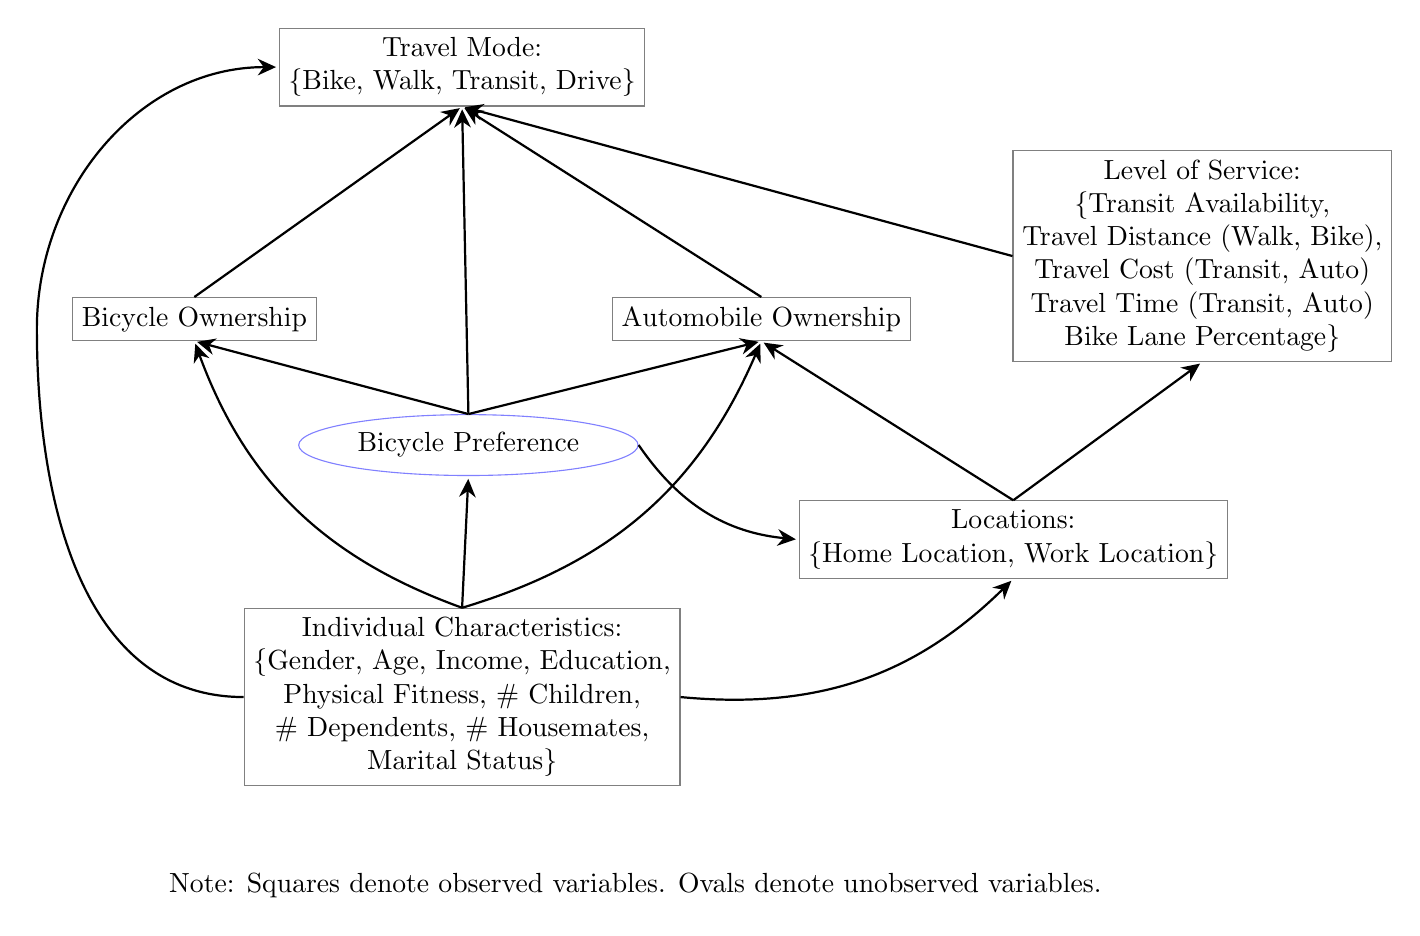
\begin{tikzpicture}
  [scale=0.8,
   bend angle=25,
   pre/.style={{Stealth[width=6pt]}-, shorten <=1pt, thick},
   post/.style={ -{Stealth[width=6pt]}, shorten >=1pt, thick},
   %latent/.style={ellipse, draw=blue!50, fill=blue!20, thick},
%   observed/.style={rectangle, draw=black!50, fill=black!20,thick}]
   latent/.style={ellipse, draw=blue!50},
   observed/.style={rectangle, draw=black!50}]

  \node[observed, align=center]   (characteristics)    at ( 1.25, -1)  {Individual Characteristics:\\\{Gender, Age, Income, Education,\\Physical Fitness, \# Children, \\\# Dependents, \# Housemates,\\Marital Status\}};
  \node[latent]         (bike-preference)  at (1.35, 3)  {Bicycle Preference};
  \node[observed, align=center]   (locations)             at ( 10, 1.5)       {Locations:\\\{Home Location, Work Location\}};
  \node[observed]   (bike-ownership)   at ( -3, 5)       {Bicycle Ownership};
  \node[observed]   (auto-ownership)  at ( 6, 5)        {Automobile Ownership};
  \node[observed, align=center]   (level-of-service)  at ( 13, 6)        {Level of Service:\\ \{Transit Availability,\\Travel Distance (Walk, Bike),\\ Travel Cost (Transit, Auto)\\Travel Time (Transit, Auto)\\Bike Lane Percentage\}};
  \node[observed, align=center]   (travel-mode)       at ( 1.25, 9)   {Travel Mode:\\\{Bike, Walk, Transit, Drive\}};
  \node                    (imaginary)          at (-5.5, 5)        {};
  
  \path[->]    (locations.north)              edge [post]    (level-of-service.south)
                                                            edge [post]    (auto-ownership.south)
                   (bike-preference.north)    edge[post]     (auto-ownership.south)
                   									 edge[post]      (bike-ownership.south)
                   									 edge[post]      (travel-mode.south)
                   (bike-preference.east)    edge[post, bend right]      (locations.west)
                   (travel-mode.south)        edge[pre]        (level-of-service.west)
                   									edge[pre]        (auto-ownership.north)
                   									edge[pre]        (bike-ownership.north)
                   (characteristics.north)    edge[post]      (bike-preference.south)
                   								    edge[post, bend right]      (auto-ownership.south)
                   								    edge[post, bend left, bend angle=45]      (bike-ownership.south)
                   (characteristics.east)      edge[post, bend right]      (locations.south)
                   (characteristics.west)    edge[-, thick, out=180, in=270]      (imaginary.south)
                   (imaginary.south)          edge[post, out=90, in=180]   (travel-mode.west);
                   
  \node             (info)     at  (4, -4) {Note:  Squares denote observed variables. Ovals denote unobserved variables.};

\end{tikzpicture}

\caption{Example Causal Diagram for Travel Mode Choice}
\label{fig:bike-causal-diagram}

\end{centering}
\end{figure}

When reading Figure \ref{fig:bike-causal-diagram}, note that the variables in the squares are observed, and the variables in ovals are unobserved. In particular, the ``bicycle preference'' node refers to a latent preference for cycling and self-identification as ``a cyclist.'' Additionally, the ``Individual Characteristics'' node and the ``Level of Service'' node denote sets of variables (given in the curly braces in each box). Each of the variables in the curly braces in these two boxes can be thought of as their own node, with the exact same ``parent nodes'' and ``child nodes.'' For instance, both bike lane percentage and transit availability are functions of home and work location, and both bike lane percentage and transit availability influence the travel mode that one chooses to commute by.

As mentioned earlier, the causal diagram encodes one's causal assumptions. For example, Figure \ref{fig:bike-causal-diagram} expresses the assumption that conditional on one's home and work locations,  individual characteristics have no effect on the level-of-service variables. However, not all causal assumptions are displayed by the diagram. One important assumption that is not explicitly shown on the diagram is that the travel mode of a given individual is not affected by the bike lane percentage for other individuals in the population. This assumption of no interference between individuals is known as the Stable Unit Treatment Value Assumption (or SUTVA for short) \citep[p.~10]{imbens2015causal}. SUTVA allows one to estimate causal effects by comparing the probability distributions of the outcomes across groups of individuals with different bike lane percentage levels. Overall, as demonstrated in this paragraph, any causal assumptions of importance that are not encoded in the causal diagram should be explicitly stated in words.


\subsubsection*{Step \ref{step:test-causal-assumptions}:}
Along with a causal diagram come a set of testable implications. Three such types of testable implications are (1) conditional independence tests, (2) tests of functional constraints, and (3) ``over-identification'' tests. First, note that our conditional independence assumptions are encoded in the causal diagram. For instance, given the causal diagram in Figure \ref{fig:bike-causal-diagram}, the following conditional independence\footnote{Note, $a \  \indep \  b \mid c$ means ``$a$ is conditionally independent of $b$ given $c$.''} assumptions are implied:
\begin{itemize}
\item $\textrm{Automobile Ownership } \indep \textrm{  Level of Service} \mid \textrm{Locations}$

\item $\textrm{Bicycle Ownership } \indep \textrm{  Level of Service} \mid \textrm{Locations}$

\item $\textrm{Individual Characteristics } \indep \textrm{  Level of Service} \mid \textrm{Locations}$
\end{itemize}
Each of these assumptions can be tested using one's actual dataset.

Secondly, in models containing latent variables, there may be ``functional constraints'' that can be tested. These constraints are basically statements that certain causal effects (i.e. certain functions) depend only on a particular subset of variables. One can then verify that this is indeed the case by ensuring that the computed causal effect is constant across different values of the variables that are supposed to have no influence on the causal effect. See \citet{tian2002testable} for more information.

Lastly, in a similar fashion, ``over-identification'' can be used when trying to falsify a given causal diagram. ``Over-identification'' refers to the situation where, given a particular causal diagram, there are two or more distinct ways to compute a given causal effect. While this is not the case in the causal diagram of Figure \ref{fig:bike-causal-diagram}, the general idea is that one computes the causal effect by all methods, and then tests for equality of the computed values. See for example \citet{sargan1958estimation, kirby2009using}.


\subsubsection*{Step \ref{step:identification-check}:}
Once one has tried and failed to falsify one's causal diagram, one can perform an identification analysis. This step is now automatic because the necessary procedures have been reduced to algorithms that are implemented in software that is freely available online. See, for example, \citet{breitling2010dagr, textor2016robust, tikka_2017_identifying}. In an observational setting, if the effects one wants to estimate (i.e. $P \left( Y_i = \textrm{bicycle} \mid \textrm{do} \left( T_i = t \right) \right)$) are identifiable, then such software will return an expression for this quantity in terms of observational distributions (i.e. distributions without the ``do'' operator) or a set of variables to be conditioned on in order to estimate the causal effect of interest. By looking at the variables contained in this expression, one will know what variables must be conditioned on, and in looking at the various probability distributions that are returned, one will know what models need to be built and estimated.

For a concrete example, see the diagram given in Figure \ref{fig:bike-causal-diagram} once more. Here, the causal effect is identified, and it is given by the following expression:
\begin{equation}
\label{eq:bike-covariate-adjustment}
P \left( Y_i = \textrm{bicycle} \mid \textrm{do} \left( T_i = t \right) \right) = \int P \left( Y_i = \textrm{bicycle} \mid T_i = t, \textrm{Locations$_i$} \right) P \left( \textrm{Locations$_i$} \mid T_i = t \right) d \left( \textrm{Locations}_i \right)
\end{equation}
From the given expression, one can see that a researcher would need to condition on the home and workplace locations of the various individuals in the dataset, and the researcher would need to build a model for the joint home and workplace location choices of the individual. Here, standard mode choice models are insufficient\footnote{As noted by an anonymous referee, it is not necessarily the case that a standard mode choice model will provide inconsistent estimates of $P \left( Y_i = \textrm{bicycle} \mid \textrm{do} \left( T_i = t \right) \right)$. However, the estimating expressions derived from the ``do-calculus'' operations on causal graphs have already been shown to sufficient for consistently estimating causal effects \citep{galles_1998_axiomatic, huang_2006_pearl}. If analysts wish to use differing expressions, then the analysts should show that their expressions also consistently estimate the desired causal effects or at least meet some other desired criteria.}. Although conventional mode choice models condition on individual characteristics, bicycle ownership, automobile ownership, and the level-of-service variables, controlling for these variables still allows for the possibility that the remaining variation in bike lane percentage is due to the ``confounding'' variable: the individual's latent bicycle preference (through one's home and work location choices). As a result, one cannot treat the observed distribution as being equal to the, desired, post-intervention distribution. We have to directly condition on the home and work locations to sever any ties between the confounding bicycle preference and the bike lane percentage\footnote{Note that if bicycle preference did not directly affect an individual's travel mode choice, then conventional travel demand models would be sufficient for estimating the effect of bicycle lane percentage on mode choice. In that hypothetical scenario, bicycle lane percentage would not be endogenous because bicycle preference would not be part of the error term.}.

\subsubsection*{Steps \ref{step:model-building} and \ref{step:post-evaluation}:}
In the previous subsection, we noted that Equation \ref{eq:bike-covariate-adjustment} called for models of the following probabilities: (1) the probability of bicycling given the bike lane percentage and one's home and work locations, and (2) the joint probability of an individual choosing his/her home and workplace locations, conditional on the bike lane percentage $t$. These models differ from typical travel demand models. The first difference is that the mode choice model, $P \left( Y_i = \textrm{bicycle} \mid T_i = t, \textrm{Locations$_i$} \right)$, conditions on far fewer variables than typical mode choice models. Secondly, the mode choice model directly conditions on the home and workplace locations instead of using proxies such as the level-of-service variables. Thirdly, the full model used to estimate the causal effect combines a joint location choice model with a mode choice model.

Differences from usual travel demand models notwithstanding, at least\footnote{There are definitely multiple sources of analytical difficulty in our example. We are not aiming to be comprehensive. If readers think of their own challenges in this example and wish to know how to address those challenges, we view this as a success for our efforts to spark consideration and discussion of causality in travel demand settings.} two problems will be encountered when trying to construct the needed models. The first issue is the fact that based on subject-matter insight, we know that even in the population, there are few individuals with the same home and workplace location. As a result, one will not have enough individuals to estimate $P \left( Y_i = \textrm{bicycle} \mid T_i = t, \textrm{Locations$_i$} \right)$ after conditioning. Secondly, even if one had multiple individuals with the same home and workplace location, the level-of-service variables such as bicycle lane percentage are a deterministic function of these two locations. There will therefore be no variation in the bike lane percentage after conditioning. Again, the requisite probabilities will not be estimable. Resolving these two issues will be key to solving the causal inference problem given in this example. Such a resolution is beyond the scope of this chapter, but we think it is instructive to identify the problem so that other researchers may join us in working on this and similar issues.

As a first step in thinking about how one might identify the causal effects of bike lane percentage on the probability of bicycling to work or school, we offer the following preliminary thoughts. First, while conditioning on variables that influence ``self-selection'' of the bike lane percentage is one way to identify the causal effect of interest, it is not the only way. The identification strategy of conditioning on the variables that lead to bike lane percentage is known as using the ``back-door criterion.'' If we can identify a variable that provides insight into the ``mechanism'' by which bike lane percentage influences an individual's travel mode, then we may be able to use the alternative ``front-door criterion'' \citep{elwert_2013_graphical, knight_2013_causal} to identify the desired causal effect. We will give an example to illustrate this alternative identification strategy. Assume that increasing an individual's bike lane percentage only influences that individual's travel mode by increasing his or her perceived sense of traffic safety for the specific commute trip by bicycle. If we are able to collect measurements of an individual's perceived sense of safety, then using integrated choice and latent variable techniques, we may be able to estimate (1) the effect of bike lane percentage on perceived safety, and (2) the effect of perceived safety on an individual's travel mode. Combining these two estimates with our assumptions, we will be able to estimate the effect of bike lane percentage on an individual's probability of traveling by bicycle. We do not claim that this is the only way to estimate the desired causal effect, or even a correct way to estimate the desired effect (since the assumptions may be incorrect), but we use the discussion as an example of how one might proceed.


Now, once one completes Step \ref{step:model-building}, one will have a model for $P \left( Y_i = \textrm{bicycle} \mid \textrm{do} \left( T_i = t \right) \right)$. This model can then be used to calculate the desired quantity:
$$E \left[ P \left( Y_i = \textrm{bicycle} \mid \textrm{do} \left( T_i = T_i ^{BL} \right) \right) - P \left( Y_i = \textrm{bicycle} \mid \textrm{do} \left( T_i = T_i ^{NBL} \right) \right) \right]$$ The end result will be a causally valid inference about the effect of the University Avenue bike lane on citywide demand for bicycle commuting.

For Step \ref{step:post-evaluation}, one should use data from actual bicycle lane interventions to corroborate the model that one is making inferences from. Note that evaluating real outcomes to see whether or not they match one's predictions has been a part of travel demand analysis from the beginning (see the discussion in Section \ref{sec:validate-inferences} about the early BART studies). While such evaluations may not be performed regularly by travel demand modelers any more, the knowledge of how to do so exists. See for example, Section \ref{sec:validate-inferences}. In the context of our example, natural experiments might take the form of measuring bicycle usage before and after the construction of bicycle lanes that are built in an ``unexpected'' manner. For instance, looking before and after the stealthy construction of bicycle lanes in New York City for public trials. We can then compare our predictions of the change in bicycle mode share before and after the installation of these lanes. Alternatively, a RCT might be analyzed whereby low-income residents applying for housing assistance are randomly placed in housing and the individuals have differing values of $T_i$. Bicycle commuting rates can then be studied using the different individuals in the program. Finally, if the bicycle lane is actually constructed on University Avenue, one should perform a post-evaluation study whereby the bicycling rates amongst residents are measured before and after the construction of the bicycle lane\footnote{Of course, care should be taken to measure bicycling rates amongst those who lived and worked in the area for a sufficiently long time before and after the construction of the bike lane. This would be done to remove any influence of individuals who may have moved their home or work location to the area after they knew the bike lane existed or was going to be built.}. Such studies will confirm whether one's model is actually performing well.

\subsection{Conclusion}
\label{sec:giving_back_to_causality}
So far, we have discussed what causal inference is, the overlapping goals of causal inference and travel demand modelling, and some reasons why we think a gulf exists between these two disciplines. Moreover, we have extracted some lessons from the causal inference literature that we think can be of use for travel demand modelers, and we have tried to show how these lessons might be used in a concrete, travel demand setting. To conclude, we now turn to the prospect of the causal inference literature being enriched by the work of travel demand modelers, and we end with a distinctly hopeful outlook.

Travel demand modeling, in its modern incarnation, grew out of the application of econometrics to the study of human travel patterns. The problems faced in modeling human travel choices are difficult, and as a result, travel demand modeling applications provided the impetus for many of the most advanced discrete choice modeling techniques to date. Concurrently, the broader field of econometrics has moved on to embrace the challenge of determining causal effects from observational and experimental data \citep{angrist2010credibility}, and we think it is only natural that travel demand modeling ``catch-up'' to its progenitor. As noted in Sections \ref{sec:why_the_disconnect} and \ref{sec:causal_lessons}, there are a number of challenges to be faced in bringing causal inference techniques and perspectives to bear on travel demand modeling applications. However, methodological challenges have always provided the most fertile ground for progress. Accordingly, we highlight three causal inference topics that we think will be particularly fruitful grounds for research and application by travel demand modelers.

First, causal inference researchers in computer science and epidemiology have been producing a small but growing literature on the topic of ``causal transportability'' and ``meta-synthesis'' \citep{hernan_2011_compound, petersen_2011_compound, pearl_2011_transportability, bareinboim_2012_transportability, pearl_2012_calculus, lee_2013_m, bareinboim_2013_transportability, singleton_2014_motivating, bareinboim_2014_transportability}. Put simply, the study of causal transportability seeks to determine the conditions and procedures with which it is possible to \textit{transport} (i.e. generalize) causal inferences learned in one setting to another \citep{pearl_2011_transportability, pearl_2014_external}. Similarly, ``meta-synthesis'' \citep{pearl_2012_calculus, lee_2013_m, bareinboim_2013_transportability, bareinboim_2014_transportability} is concerned with the formalization of procedures for combining inferences from multiple studies into one aggregated measure for a target population that need not have been involved in any of the studies being combined. Thus far, papers about causal transportability have mainly focused on the abstract mathematical conditions that permit the transport of causal inferences. There has been a comparative lack of research applying the knowledge obtained thus far to real applications\footnote{Notable exceptions include work such as \citet{singleton_2014_motivating}.}. There is likely much to be gained from applying the abstract mathematics of causal transportability research to real problems and from attempting to integrate transportability notions with domain specific modeling techniques and traditions. Already, travel demand modelers have much experience with two specific transportability processes: (1) transferring model results from one time and place to another \citep{agyemang_1997_spatial, fox_2015_temporal}, and (2) generalizing insights from stated preference (SP) experiments to revealed preference (RP) studies. In the latter case, travel demand studies have used a number of techniques to facilitate the desired transport of model results. For example, these techniques include methods such as joint RP-SP estimation techniques \citep{brownstone_2000_joint, feit_2010_reality}, incentive-aligned SP experiments to increase the similarity between the SP study and the RP environment where the results will be used \citep{ding_2005_incentive, ding_2007_incentive, moser_2010_using, chung_2017_willingness}, and certainty calibration \citep{beck_2016_can}. From both model transferability and RP/SP studies, travel demand modelers may have much accumulated wisdom to offer the causal transportability literature. Conversely, travel demand modelers may also have much to gain by incorporating the existing causal transportability techniques, especially when trying to determine whether or not the desired inferential transport can actually be performed.

Secondly, feedback processes and change over time have been ignored in much of the causal inference research performed thus far\footnote{Thanks to two anonymous referees for raising this point.}. Indeed, much of the causal inference work performed thus far takes the directed \textit{acyclic} graph as its starting point (or equivalently, the \textit{recursive} structural equation model used in much of the social sciences). Such work explicitly excludes systems of relationships where variable 1 both causes and is affected by variable 2 (possibly offset by a time lag). A transportation example of such a feedback process is where an individual's attitudes towards bicycling affect the individual's choice of bicycling or not, but the individual's experiences while bicycling will then affect his/her future attitudes towards bicycling. While possibly a rare occurrence in other disciplines, we expect that such feedback processes are common in travel demand settings. As another example, consider the effect of increased driving costs. At the outset, the increase in costs is expected to damp demand by some initial amount. However, the initial decrease in the number of drivers may alleviate congestion, thereby causing an increase in traffic speeds and leading some potential drivers to begin driving due to the faster speeds. The overall decrease in the number of drivers will therefore be less than the initial decrease due to the increased prices. This overall decrease in the number of drivers may be over-predicted if the feedback mechanism is ignored. To give credit where it is due, a limited amount of causal inference work has tried to account for such feedback processes. This work includes the use of chain graphs \citep{lauritzen_2002_chain}, directed \textit{cyclic} graphs \citep{schmidt_2009_modeling}, the ``settable systems'' framework developed by econometricians Halbert White and Karim Chalak (\citeyear{white_2009_settable}), and dynamic causal networks \citep{blondel_2017_identifiability}. However, as with the aforementioned causal transportability studies, these techniques have seldom been used in real applications. Here, travel demand modelers would essentially forge the link between systems dynamics researchers who commonly use causal diagrams to portray systems with feedback processes over time (for example \citet{abbas_1994_system} and \citet{shepherd_2014_review}) and causal inference researchers who use causal diagrams to explicitly identify and compute causal effects.

Finally, travel demand researchers face severe challenges when trying to make robust quantitative claims. The fragility of travel demand modeling results often comes from ambiguity over how to choose the variables to be conditioned on when trying to estimate the probability of interest, how to specify the ``systematic utility'' equations\footnote{We realize that not all travel demand models have systematic utilities. However, given that most travel demand models are based on random utility maximization, the comments in this paragraph are valid for most travel demand analyses.}, how the preferences underlying the systematic utilities might change over time, how to specify the probability function that links the systematic utilities with the probability of the observed choice, and even ambiguity in the causal diagram upon which the entire analysis should be built (for e.g. see the literature on observationally equivalent causal graphs). As was recently noted by Dagsvik:
\begin{quotation}
``A well-known problem in quantitative economic analysis is that economic theory provides limited guidance for the specification of functional forms of quantitative structural economic models. An unfortunate consequence is that it becomes difficult to discriminate between econometric model formulations based on the same theoretical framework which fit the data reasonably well but result in different counterfactual predictions. Given this state of affairs, the analyst is forced to choose between model specifications without adequate theoretical or empirical support.''--\citep{dagsvik_2017_invariance}
\end{quotation}
Overall, we believe that this ambiguity in travel demand models will remain for the foreseeable future. So although the type of sensitivity analysis advocated in Section \ref{sec:validate-inferences} will help uncover how much uncertainty in one's estimates there actually is, one will likely always need good methods of reporting this uncertainty. Here, we have seen few \textit{structural} causal inference studies that managed to present the uncertainty inherent in their analysis in an easy to understand and useful manner. In our opinion, the inherent ambiguity in travel demand models gives transportation researchers an opportunity to take the lead on discovering parsimonious and meaningful ways of representing the uncertainty in one's analysis.

In conclusion, if the past is any indication of the future, then based on the topics above, we believe that travel demand modelers will once again be able to advance the arsenal of quantitative techniques, this time in the causal inference arena as opposed to simply in the arena of discrete choice. By generalizing and adapting causal inference techniques for travel demand applications, travel modelers can simultaneously contribute to the field of causal inference and fulfill their original purpose of \textit{validly} ``predict[ing] the consequences of alternative policies or plans [...] under radically different conditions'' than those present at the time of one's analysis.

\section{Acknowledgements}
We thank Elias Barenboim, Kenneth Train, Eric Miller, Mohamed Amine Bouzaghrane, and Hassan Obeid for comments on earlier drafts of this chapter, and we thank Michael Anderson for providing us with early introductions to the topic of causal inference. We are also very grateful to anonymous reviewers for their thoughtful and detailed comments on an earlier draft of this chapter. Nevertheless, all viewpoints (and, of course, any errors) expressed in this chapter are entirely our own.

\newpage
\renewcommand\bibname{{References}} %  will print ''REFERENCES'' instead of ''BIBLIOGRAPHY''
\bibliographystyle{plainnat}
\bibliography{chapter5/current/ch5}


%\clearpage
%!TEX root = chapter5/../dissertation.tex

\chapter{Conclusion}
\label{ch:6}

\section{Research Overview}
In this dissertation, I made two broad types of advances. The first type of advances are substantive: I developed new bicycle demand models. These new models address three bicycle-specific concerns: incorporating important but frequently ignored roadway-level variables, allowing for differential rates of ``abandonment'' between bicycling and other travel modes, and reflecting the likely reality that individuals use non-compensatory or semi-compensatory decision rules to decide whether they will commute via bicycle.

The second type of advances are methodological. Here, I blended traditional discrete choice models with methods from statistics, machine learning, and causal inference. Specifically, I used statistical techniques to create a new class of finite-parameter, closed-form, asymmetric choice models. Next, I detailed a micro-economic framework for interpreting decision tree models from machine learning, and I created new, semi-compensatory choice models using the proposed framework. Lastly, through the lens of causal inference, I examined travel demand modeling overall and a bicycle demand modeling problem in particular. These examinations led to the recognition that, as a field, we discrete choice modellers still need to make significant methodological changes to our travel demand models (bicycle demand models being included as a subset). The validity of our work is questionable without such changes.

Together, these substantive and methodological advances have three main impacts. First, transportation analyst have more accurate and more realistic bicycle demand models for use in their jurisdictions. Second, discrete choice modellers have more accurate, flexible, and micro-economically diverse models for their various applications. And finally, discrete choice researchers have new frameworks for interacting with the fields of statistics, machine learning, and causal inference.

The remaining sections return to these points and will proceed as follows. First, I will provide a more detailed recap of the contributions I made in this dissertation. Next, I will note the limitations of my efforts. And finally, building off these limitations and looking at future opportunities, I will note some research directions that seem especially promising and/or needed.

\section{Research Contributions}
This dissertation is composed of four primary research efforts. Each of these efforts makes both substantive (i.e. bicycle-planning-focused) contributions and methodological ones. Below, I describe these contributions, one project at a time.

First, I developed a method for incorporating roadway-level variables (e.g. speed limits, slopes, the presence of bike lanes, ``share the road arrows'' (sharrows), etc.) into travel demand models. This methodology relies upon a novel concept termed the ``zone-of-likely-travel'' and decision trees from computer science. The basic idea of the zone-of-likely-travel is that it is a polygon that represents a geographic buffer around the shortest-path from one's origin to one's destination. However, this buffer is constrained to follow the roadway network instead of merely being laid over it, and the size of the buffer is such that an individual who cycles is likely to take a path that is within the buffer. For all roadways within the zone-of-likely-travel, the desired spatial variables are recorded, then these variables are aggregated to the level of the zone by taking averages and percentiles. Finally, a decision tree is built using a dependent variable of ``bicycle or not,'' representing whether the individual commuted to work or school by bike. The nodes of the decision tree are used as descriptors of each zone-of-likely-travel.

Theoretically, this variable incorporation procedure blends existing ``buffer-based'' methods with objectively created ``bicycle environment factors.'' Substantively, my new procedures avoids drawbacks of these earlier methods (and procedures based on route choice models). In particular, My zones are constructed to lie between one's origin and destination, so it excludes roadways that are not in the direction one would travel, and it includes roadways that may be left out by disjoint buffers around one's origin and destination. Moreover, it creates descriptors of the bicycling environment in an objective fashion that is tailored towards predicting bicycle demand. And finally, this method avoids the pitfall of route-choice models, which is that they are built solely on cyclists and then extrapolated to the entire population of cyclists and non-cyclists alike. Methodologically, I created a new method for improving the accuracy of bicycle demand models, and I provided another example of the successful and complementary combination of decision trees and discrete choice models.

% Asymmetric
Next, I created a class of asymmetric, multinomial discrete choice models with a finite number of parameters. This class of ``logit-type'' models has the substantive affect of allowing analysts to model the (a-priori likely) situation where individuals have differing rates of adoption or abandonment of depending on the travel mode being examined. For instance, from a state of indifference, an individual's probability of commuting by bicycle may fall quickly with respect to a change in its systematic utility. In contrast, an individual's probability of driving may fall less rapidly with an equal change in the systematic utility of driving. Empirically, this new class of models made more accurate predictions than standard, symmetric discrete choice models.

Methodologically, this extension makes a number of contributions to the discrete choice literature. First, such models provide a more flexible way to explain observed levels of class-imbalance as opposed to solely relying on one's alternative specific constants. Secondly, the new class of logit-type models generalizes a wide variety of existing, binary asymmetric models to the multinomial setting for the first time, making such models immediately useful to transportation, marketing, and other disciplines where individuals choose between multiple (i.e. more than two) alternatives. Third, I also introduced procedures for systematically creating new asymmetric choice models. This allows researchers to create new asymmetric models that are tailored to the specific desired qualities.

% Economics of Decision Trees
For my third project, I detailed a micro-economic framework for the interpretation of decision tree models from computer science. At a practical level, motivated by this new framework, I created a bayesian model tree that places a discrete choice model inside a decision tree, and performs a bayesian estimation of this entire system. Substantively, these expansions allow one to capture non-compensatory and context-dependent semi-compensatory decision making amongst individuals. Based on qualitative and anecdotal reports, these effects are expected to be significant for the choice of bicycle commuting. This intuition was supported in the empirical application of our bayesian model trees. The bayesian model tree model had dramatically better levels of fit than a standard MNL model, and the insights and forecasts of the bayesian model trees were far more plausible than those offered by the MNL model.

Methodologically, I merged an existing class of machine learning models (decision trees) with economic theory. This should be greatly helpful in promoting the use and advancement of tree-based models by discrete choice modelers and other researchers that come from a background in econometrics. By relying on tree-based models, I provided a model for very flexible non-compensatory decision rules that generalize those used in the discrete-choice literature so far. At the same time, tree-based models avoid theoretical drawbacks of previous research methods such as the ability to make predictions for all future scenarios. Lastly, I methodologically contribute to the literature on tree-based models by developing the first model that simultaneously allows for estimation uncertainty (through the bayesian estimation) and context-dependent preference heterogeneity (through the model trees).

% Causal Inference in Travel Demand Modeling
For this dissertation's final project, I examined travel demand modeling procedures through the perspective of the causal inference literature. Because these two fields have different methods but largely overlapping goals, I was able to use causal inference results to identify inferential practices within the travel demand modeling practices that are likely to be invalid. Substantively, this project resulted in the recognition of the overwhelming need for bicycle demand models to address the issue of unmeasured confounding. Without doing so, analyses and plans based on bicycle demand models that are estimated from observational data should be viewed with suspicion.

Methodologically, this project pointed toward a number of causal inference practices that could immediately benefit the field of travel demand modeling. Such practices include the unambiguous stating of causal assumptions for a given study. These statements should include, but not be limited to, drawing causal diagrams. Moreover, helpful causal inference practices would also include techniques such as making greater use of models with fewer assumptions (e.g. non-parametric models) and checking the validity of one's model predictions using techniques such as before-after studies, natural experiments,difference-in-difference studies, and randomized controlled trials. At the same time, this project uncovered ways that travel demand modelers could contribute to the causal inference literature. Such ways include taking the lead on studies of causal transportability, studies including feedback processes, and the representation of analytic uncertainty in all its forms. These are all topics where transportation researchers have either done much work or they are working conditions that travel demand modelers are forced to face, for better or for worse. By tackling the causality issues inherent in such studies, travel demand modelers can increase the validity of their own work and improve the state of causal inference knowledge overall.

\section{Research Limitations}
Overall, my research efforts in this dissertation suffer from two main drawbacks. First, many of the new techniques require ad-hoc decisions on the part of the researcher. For instance, the zone-of-likely-travel requires a researcher to choose a percentile between 0 and 100 to approximate the distribution of how far cyclists are willing to deviate from their shortest paths. To develop new asymmetric choice models, my procedures require an individual to choose a loss function from which the new model will be derived. There are few principled guidelines for choosing a specific loss function. As a final example, my proposed estimation procedures for bayesian model trees required the choice of a small number of individual decision trees to represent the full posterior distribution of trees. In this dissertation, I chose the trees in an ad-hoc manner that, while practically successful in the current research setting, does not provide guiding principles that are proven to be successful in more general settings.

Secondly, the methods developed in this dissertation require a substantial effort for use in new settings. For instance, an analyst seeking to use my zone-of-likely-travel ideas may have to program their own routines to construct the zones. The routines used in this research were ``minimally-viable-products'' that worked for my contexts (i.e. the cities being used in my research, the origin-destination pairs observed in my datasets, etc.). However, my routines are neither robust nor computationally efficient. Likewise, for any asymmetric choice models developed using this dissertation's techniques, beyond the four that I have already created, one will have to program the models without being able to rely on existing implementations. Given that ``the devil is in the details,'' the way that a new researcher implements the estimation code for the new asymmetric models may have a significant effect on the apparent success of the new model. Finally, the bayesian model trees that I created in this dissertation require numerous choices of priors, of choice model ``kernel'' (I used an MNL model, but one can use any discrete choice model more generally), and of the type of decision tree being used. Since these different choices can lead to vastly different code to implement such models, new researchers will have to perform such implementations themselves. Such implementation may seem daunting, and may therefore discourage the most appropriate and flexible use of these new techniques.

Despite the points above, one could argue that the obligation of researchers is to produce new ideas, not necessarily to produce commercial-grade implementations of these ideas. In this sense, the aforementioned issues are unfortunate realities of my work, as opposed to limitations. However, my opinion is that since researchers are often funded by the public (through government grants), researchers should strive to make their work as useful as possible to the public. This means making research as easy to use by others as possible. Accordingly, the next section begins with this goal, recommending future research directions that (1) address the limitations mentioned in the preceding paragraphs and (2) leverage the work in this dissertation to address problems that I believe are of the utmost importance for discrete choice modelling in general, and for bicycle demand modelling in particular. 

\section{Recommendations for Future Research}
As noted above, this section will make two general types of recommendations for future research. The first type of recommendation will focus on how to improve the techniques created in earlier chapters. The second type of recommendation will focus on new issues, beyond those that were investigated in this dissertation. Lastly, in addition to the recommendations below, each of the dissertation chapters contains its own set of further research directions (many of which are unique from those described below).

Now, beginning with the bicycle focused research, it is likely that some analysts will encounter difficulties when constructing zones-of-likely-travel due to computational speed or due to the complexities of real, digital roadway network files. Future research efforts should therefore focus on creating computationally efficient and robust\footnote{Note that I mean robust to different roadway network configurations.} procedures for creating the zones-of-likely-travel. This would enable individuals to reap all the theoretical benefits of this method's approach to incorporating roadway-level variables into travel demand models.

Next, future research should investigate the relationship between intrinsic features of one's dataset and the type of shapes that one's asymmetric choice model should have in order to generate the most accurate predictions. Such research would guild the selection of loss functions from which one can derive the desired choice model, and it would help analysts who, reasonably, may not be familiar with the various types of loss functions in existence. Similarly, future research should investigate how tools such as automatic differentiation and computational graphs can be used to unify and streamline the implementation of such asymmetric choice models.

Finally, my last recommendation for improving this dissertation's research is that future efforts should create numerically robust, conceptually streamlined, and computationally fast estimation methods for bayesian model trees. Ideally, such estimation methods will be `one-step' methods as opposed to the three-step methodology used in this dissertation. An estimation technique of this kind would greatly reduce the trepidation that some modellers may experience when thinking of using a new choice model.

To conclude, I will three highlight research recommendations that I believe are more `forward-facing,' as opposed to being primarily focused on improving this dissertation's efforts. First, one of the most exciting research topics that was not explored in this dissertation is the effect of using asymmetric choice models as the class-membership models in a latent-class framework. Here, the asymmetric choice models would provide information on how difficult it is to switch members of the population from one latent-class to another. If the latent-classes capture behavioral heterogeneities such as differing choice-sets and taste-parameters, then such asymmetric latent-class models may entail drastically different policy implications than our current models. For instance, we may find that radically more aggressive policy changes are needed to switch individuals into a latent market-segment that considers `active' transportation modes. Alternatively, we may discover that certain latent classes are easily affected by policy changes, thus warranting a greater focus on these groups than would have been given when using a traditional latent-class model.

Secondly, as noted in the chapter on causal inference, unmeasured confounders greatly increase the difficulty of drawing causal inferences from observational data. To date, researchers (both in and outside of discrete choice) have not figured out how to mitigate the effects of unmeasured confounding in general settings. To make matters worse, the presence of unobserved confounding is likely the rule, as opposed to the exception, in observational studies. Given this state of affairs, it behooves discrete choice modelers to attack the problem of modeling in the presence of unobserved confounding. Without progress on this front, it is unlikely that our profession has any hope of performing defensible policy analyses based on observational data.

Lastly, my final recommendation is emblematic of this dissertation overall, as it is both methodological in nature and substantively focused on the issue of bicycle planning. Thus far, most transportation planning agencies act in a ``reactive'' manner. In the (unfortunately) unlikely scenario that a planning agency has a bicycle mode share goal, the agency will likely first come up with a set of plans for bicycle infrastructure investment. Only afterwards will the agency (at best) check to see whether the plan is expected to increase bicycle demand levels to the desired amounts. I believe that this order of operations should be reversed. Given a budget constraint, agencies should proactively optimize the placement of bicycle infrastructure to maximize the expected bicycle mode share. Methodologically, this requires (1) causally valid bicycle demand models, and (2) optimization techniques that treat demand as the objective function while being able to handle huge amounts of boolean decision variables (e.g. bike lane on this street or not). Such a collaboration between optimization experts and discrete choice modellers has yet to be realized, but to best manage public funds, this type of joint research should be a priority for future efforts.

% \appendix
% \chapter{More Monticello Candidates}

%\bibliographystyle{plainnat}
%\bibliography{dissertation}

\end{document}
